%!TeX root=../tese.tex
%("dica" para o editor de texto: este arquivo é parte de um documento maior)
% para saber mais: https://tex.stackexchange.com/q/78101/183146

% Apague as duas linhas abaixo (elas servem apenas para gerar um
% aviso no arquivo PDF quando não há nenhum dado a imprimir) e
% insira aqui o conteúdo dos apêndices do seu trabalho (ou deixe
% este arquivo vazio)

% Os apêndices podem ser inseridos diretamente aqui ou "puxados" de outros
% arquivos.
% Em alguns (raros) casos, pode ser interessante usar \include ao
% invés de \input: https://tex.stackexchange.com/a/32058/183146

%\input{conteudo/...}
%\par

%\providecommand\aviso[1]{
  \clearpage
  \null
  \vfill
  \begin{hyphenrules}{nohyphenation}
    \centering\bfseries\Large
    #1\par
  \end{hyphenrules}
  \vfill
  \clearpage
}

\providecommand\avisoFolhasDeRosto{
  \aviso{
    {\huge Você precisa editar os arquivos no diretório ``\texttt{conteudo}''!}
    \par\bigskip\bigskip\bigskip\bigskip
    Para gerar a capa e demais páginas preliminares no formato correto,
    modifique os arquivos ``\texttt{conteudo/paginas-preliminares.tex}'' e
    ``\texttt{conteudo/metadados.tex}'', usando como base os arquivos
    correspondentes no diretório ``\texttt{conteudo-exemplo}''.
  }
}

\providecommand\avisoCapitulos{
  \aviso{
    Insira o conteúdo dos capítulos do seu trabalho no arquivo
    ``\texttt{capitulos.tex}'' do diretório ``\texttt{conteudo}''.
  }
}

\providecommand\avisoApendices{
  \aviso{
    Insira o conteúdo dos apêndices do seu trabalho no arquivo
    ``\texttt{apendices.tex}'' do diretório ``\texttt{conteudo}''
    (ou comente a linha correspondente em \texttt{tese.tex}).
  }
}

\providecommand\avisoAnexos{
  \aviso{
    Insira o conteúdo dos anexos do seu trabalho no arquivo
    ``\texttt{anexos.tex}'' do diretório ``\texttt{conteudo}''
    (ou comente a linha correspondente em \texttt{tese.tex}).
  }
}

\providecommand\avisoArtigo{
  \aviso{
    Insira o conteúdo do artigo no arquivo ``\texttt{corpo-artigo.tex}''
    do diretório ``\texttt{conteudo}''. Não se esqueça de consultar
    o exemplo no diretório ``\texttt{conteudo-exemplo}'' para a
    definição do título, autoria etc.
  }
}

\providecommand\avisoApresentacao{
  \begin{frame}{Insira o conteúdo!}
  \aviso{
    Insira o conteúdo da apresentação no arquivo ``\texttt{corpo-apresentacao.tex}''
    do diretório ``\texttt{conteudo}''. Não se esqueça de consultar
    o exemplo no diretório ``\texttt{conteudo-exemplo}'' para a
    definição do título, autoria, estrutura etc.
  }
  \end{frame}
}

\providecommand\avisoPoster{
  \aviso{
    Insira o conteúdo do poster no arquivo ``\texttt{corpo-poster.tex}''
    do diretório ``\texttt{conteudo}''. Não se esqueça de consultar
    o exemplo no diretório ``\texttt{conteudo-exemplo}'' para a
    definição do título, autoria, estrutura etc.
  }
}

%\avisoApendices



%% ------------------------------------------------------------------------- %%
\chapter{Moda das Ondas no Tower Defense para versão v1}
\label{sec:apend-moda-td-v1}

Foram calculadas as modas das ondas do \textit{fitness} desenvolvido, para permitir a visualização dos inimigos mais comuns que o algoritmo convergiu.

%% ------------------------------------------------------------------------- %%
\section{Torres Verdes}
\label{sec:apend-moda-td-g-v1}

\begin{figure}[H]
  \centering
  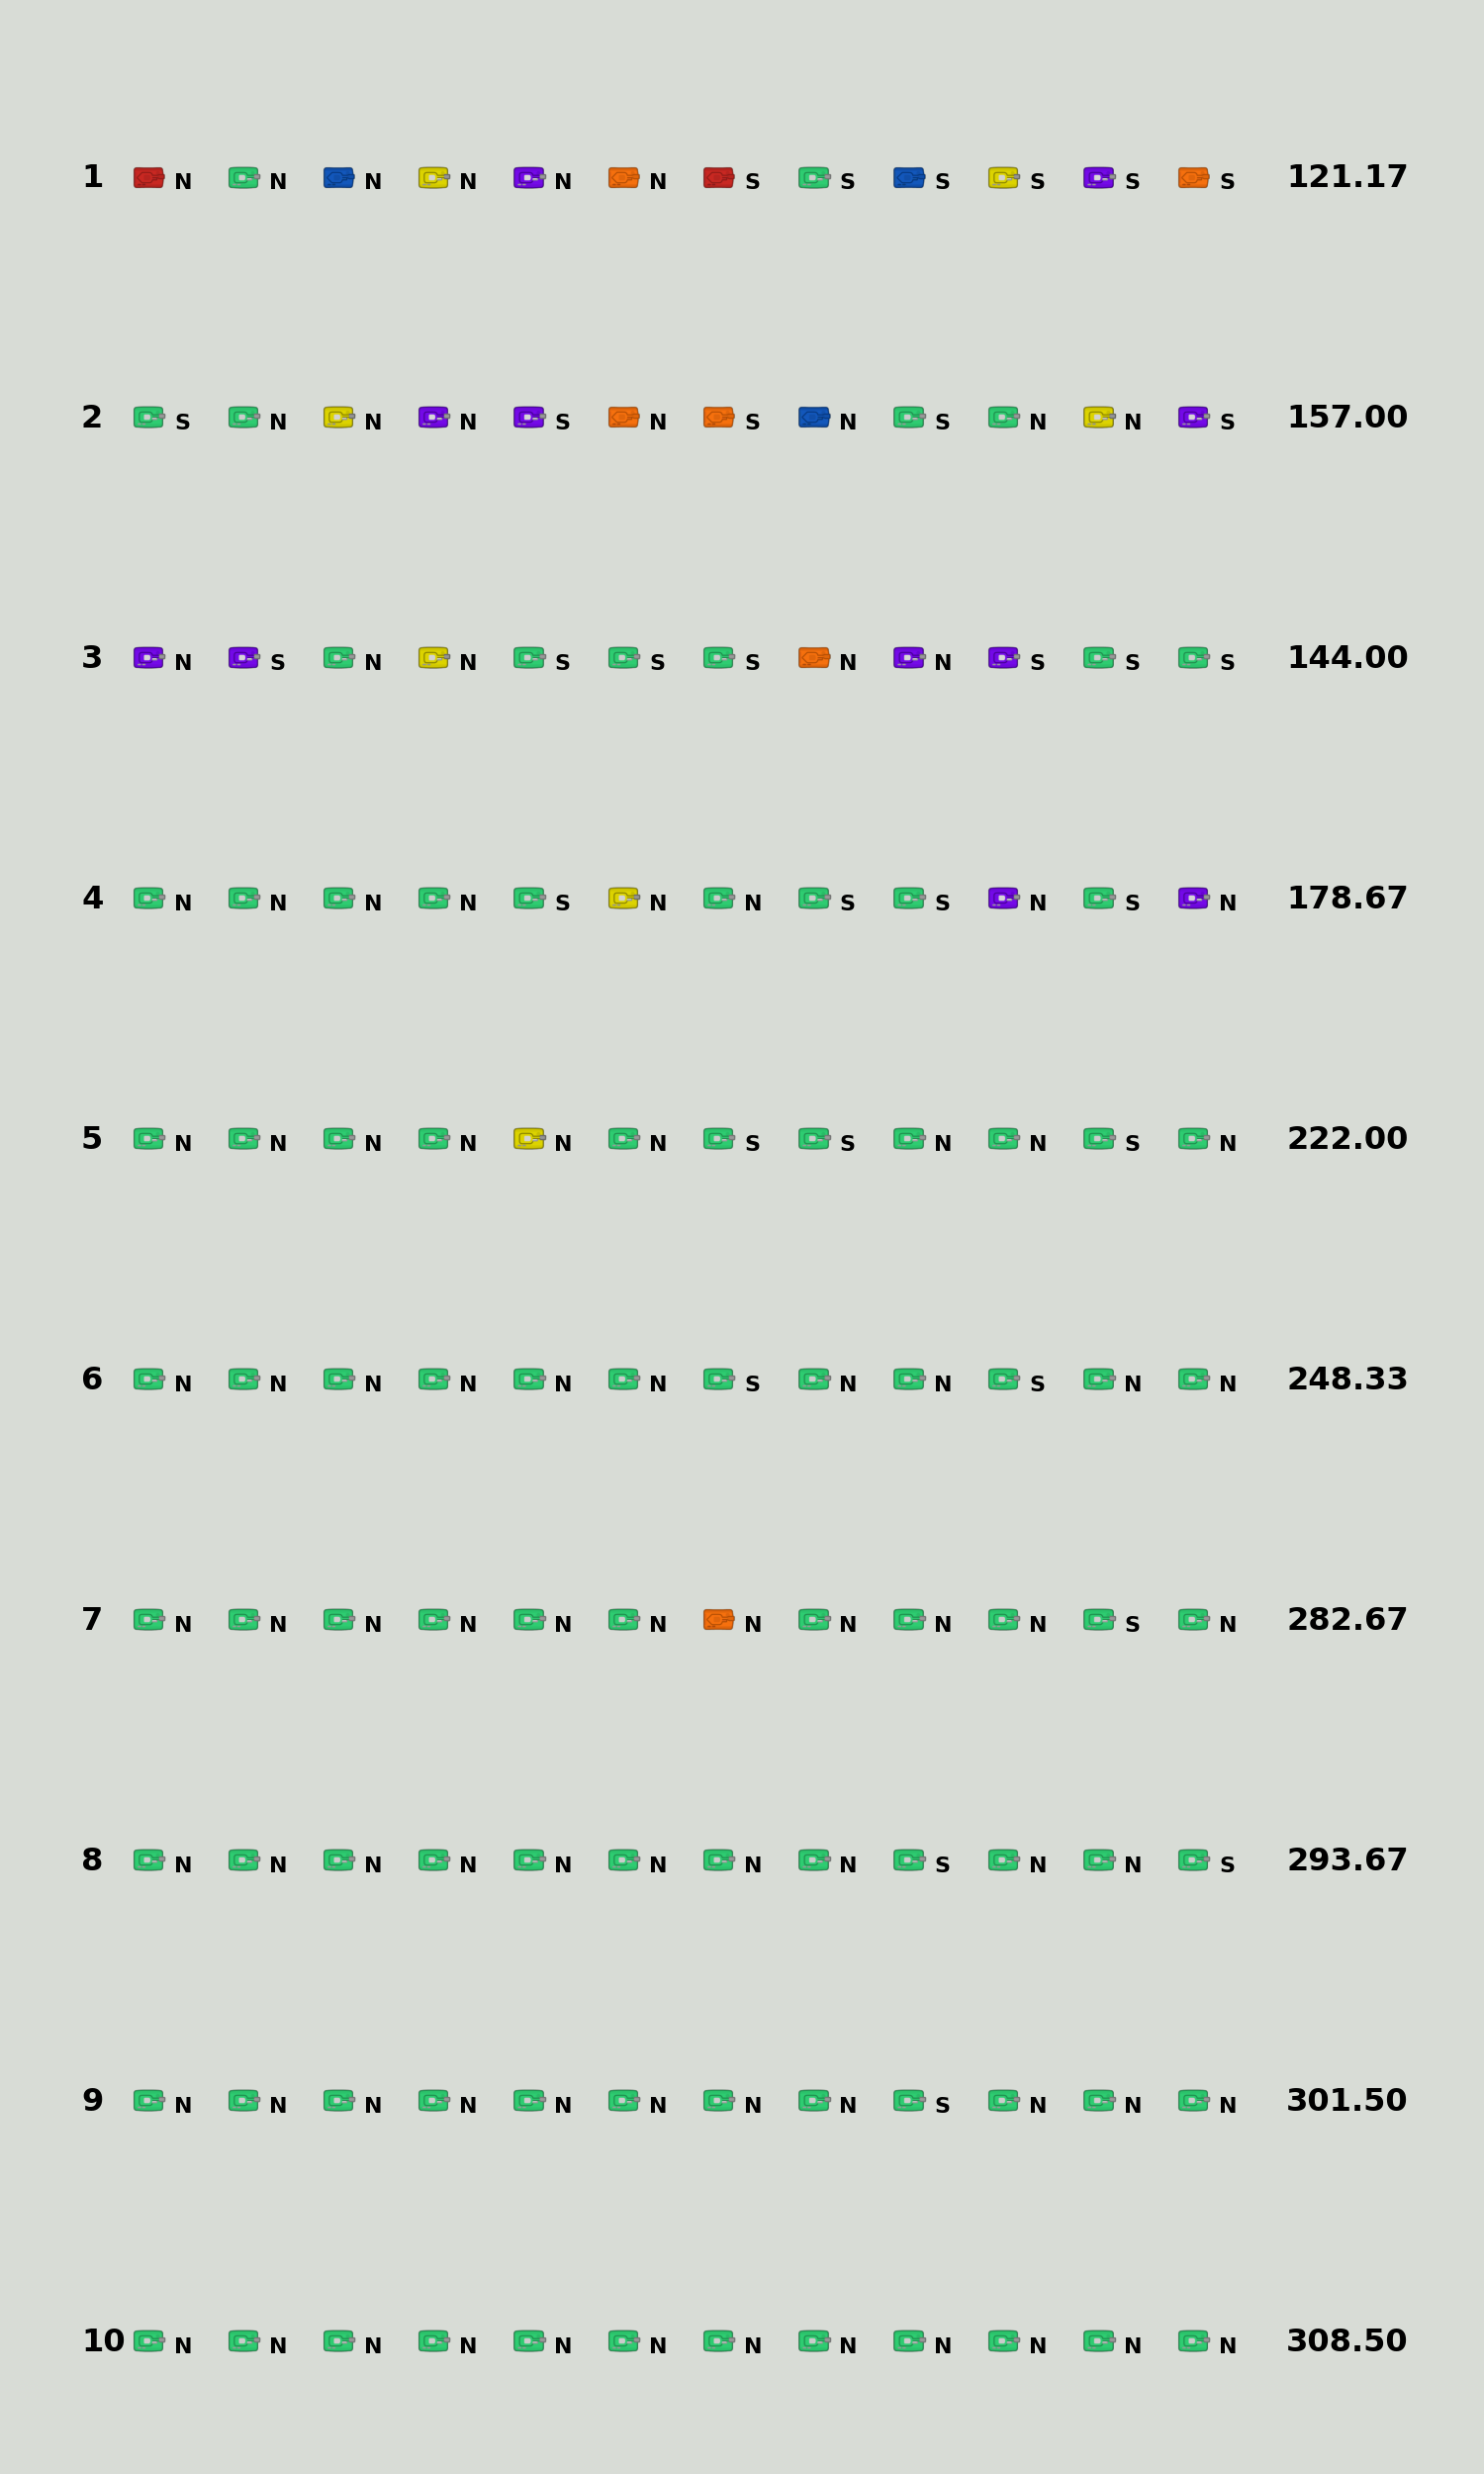
\includegraphics[width=0.9\textwidth]{figuras/td/td_allgreen_ai_mode_1_1.png}
  \caption{Visualização da moda de cada onda com a versão v1 contra Torres Verdes.}
  \label{fig:td-moda-green-1-1}
\end{figure}

\begin{figure}[H]
  \centering
  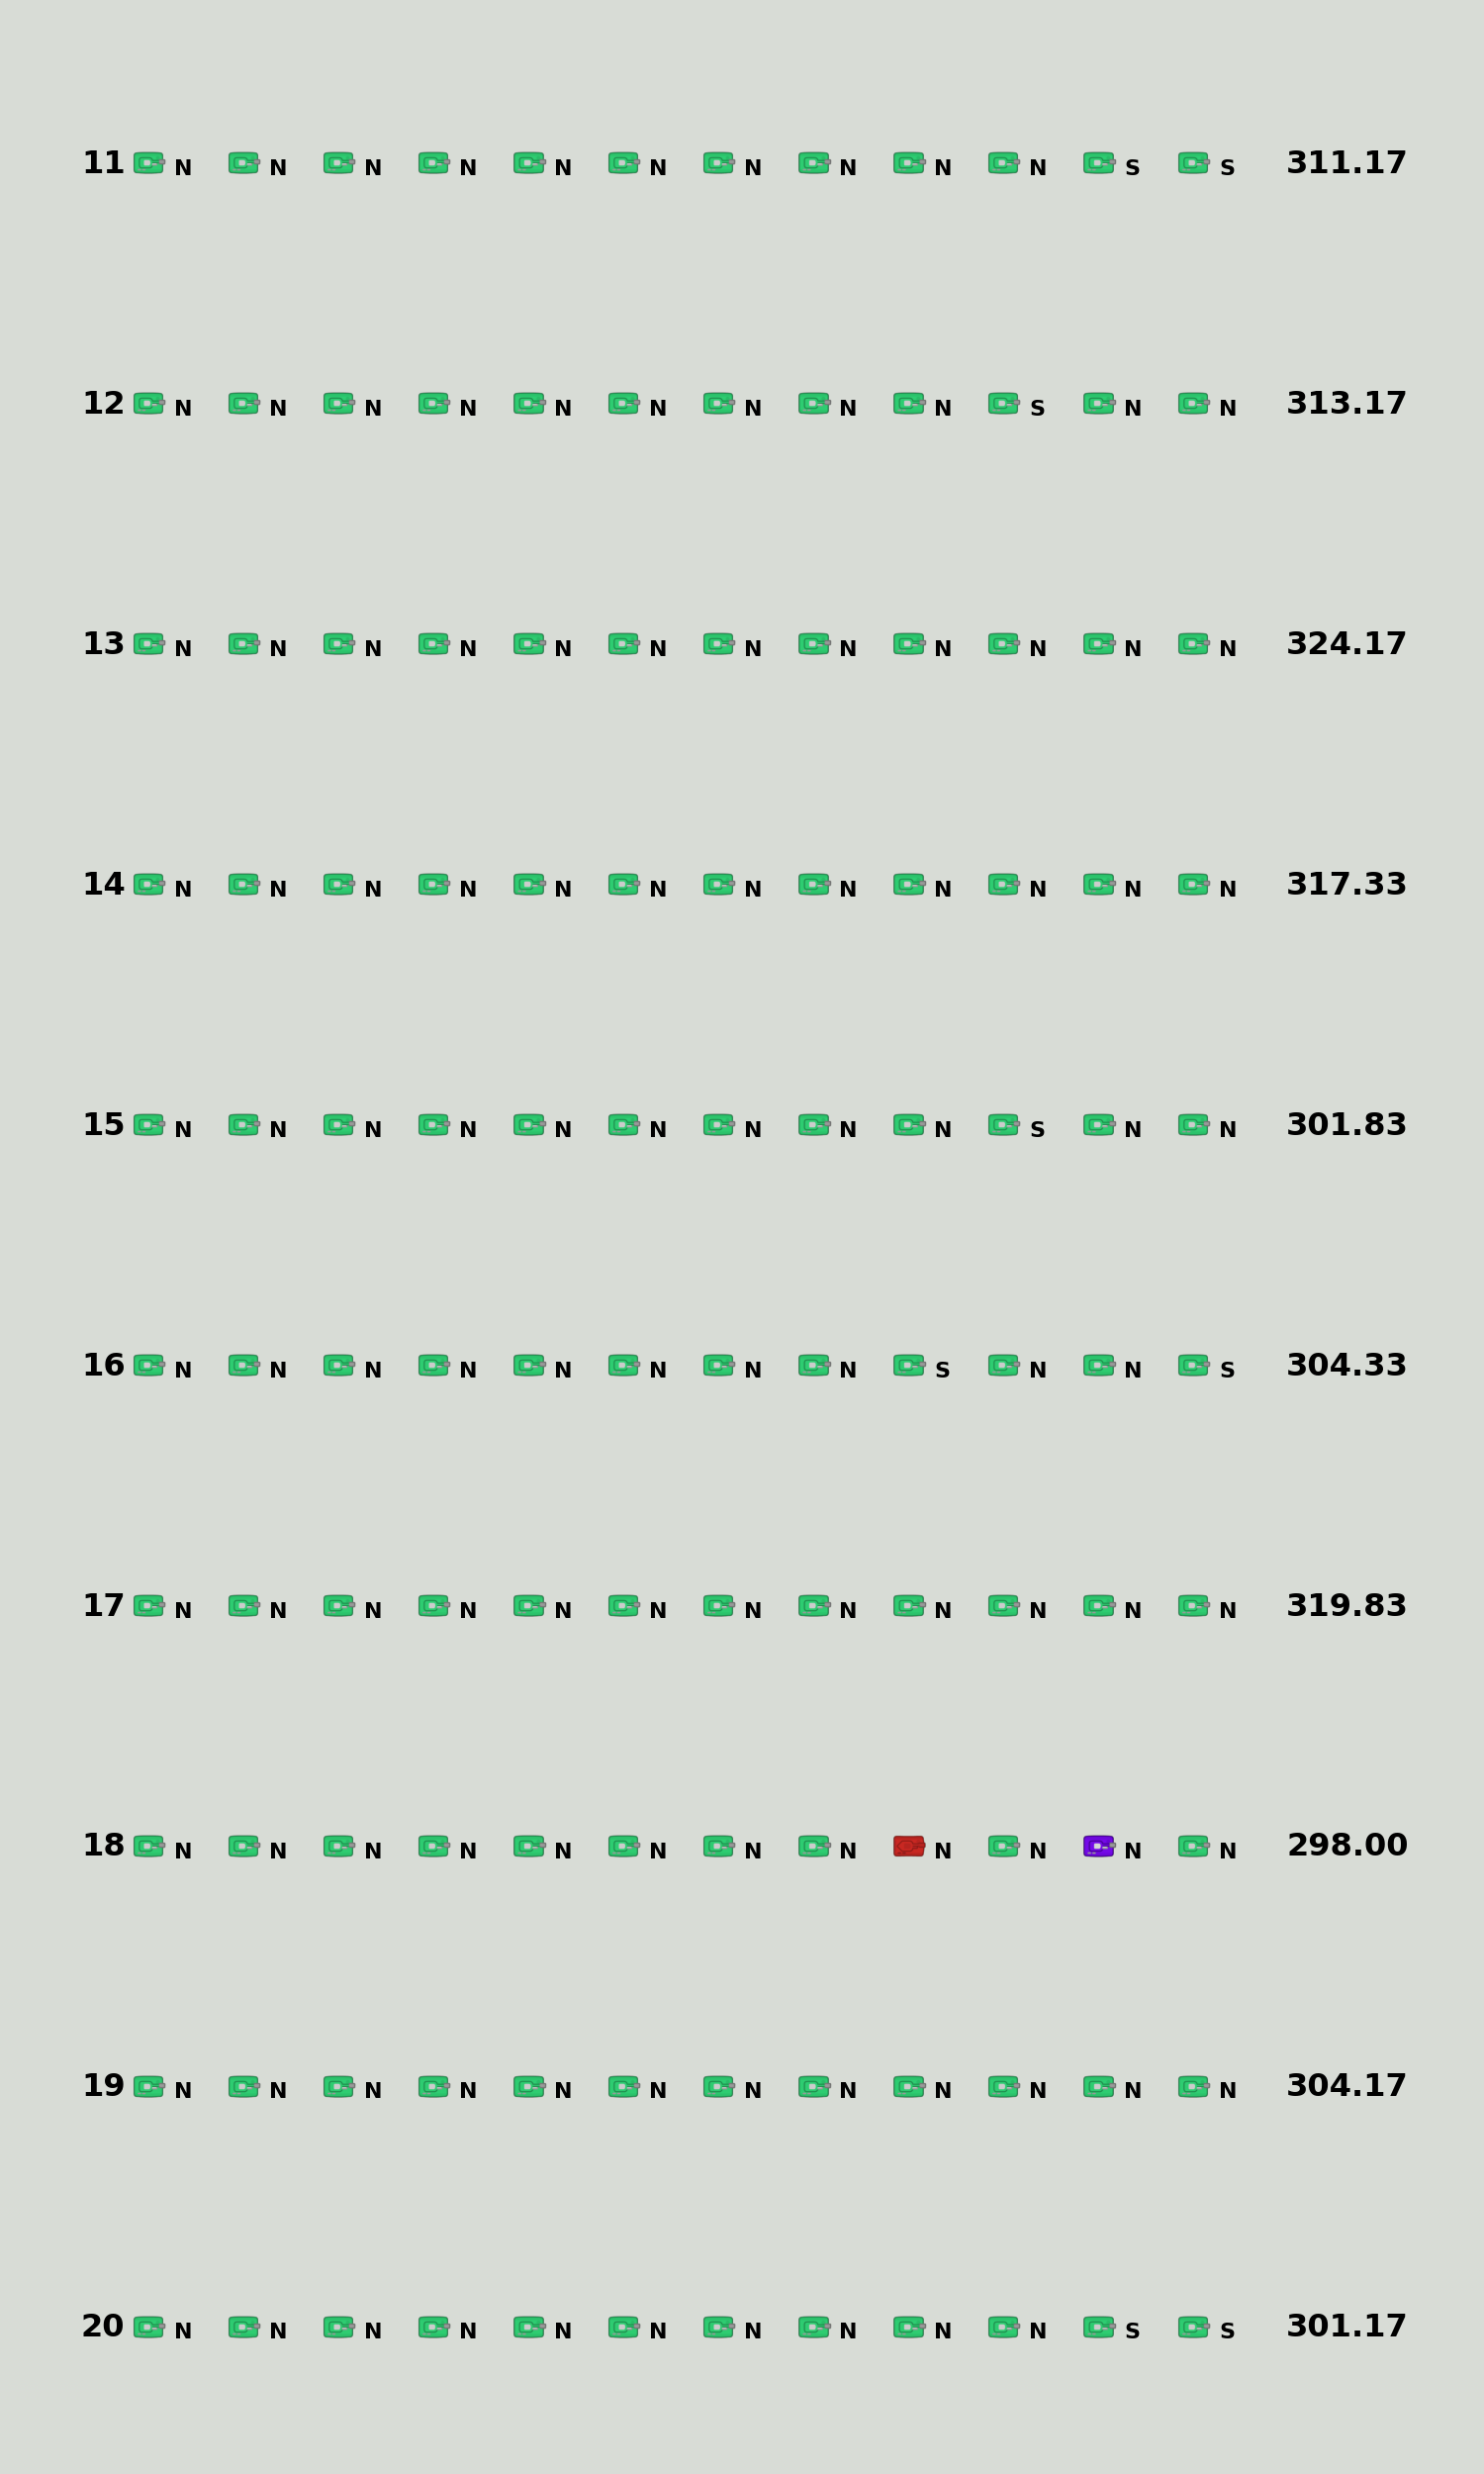
\includegraphics[width=0.9\textwidth]{figuras/td/td_allgreen_ai_mode_1_2.png}
  \caption{Visualização da moda de cada onda com a versão v1 contra Torres Verdes.}
  \label{fig:td-moda-green-1-2}
\end{figure}

\begin{figure}[H]
  \centering
  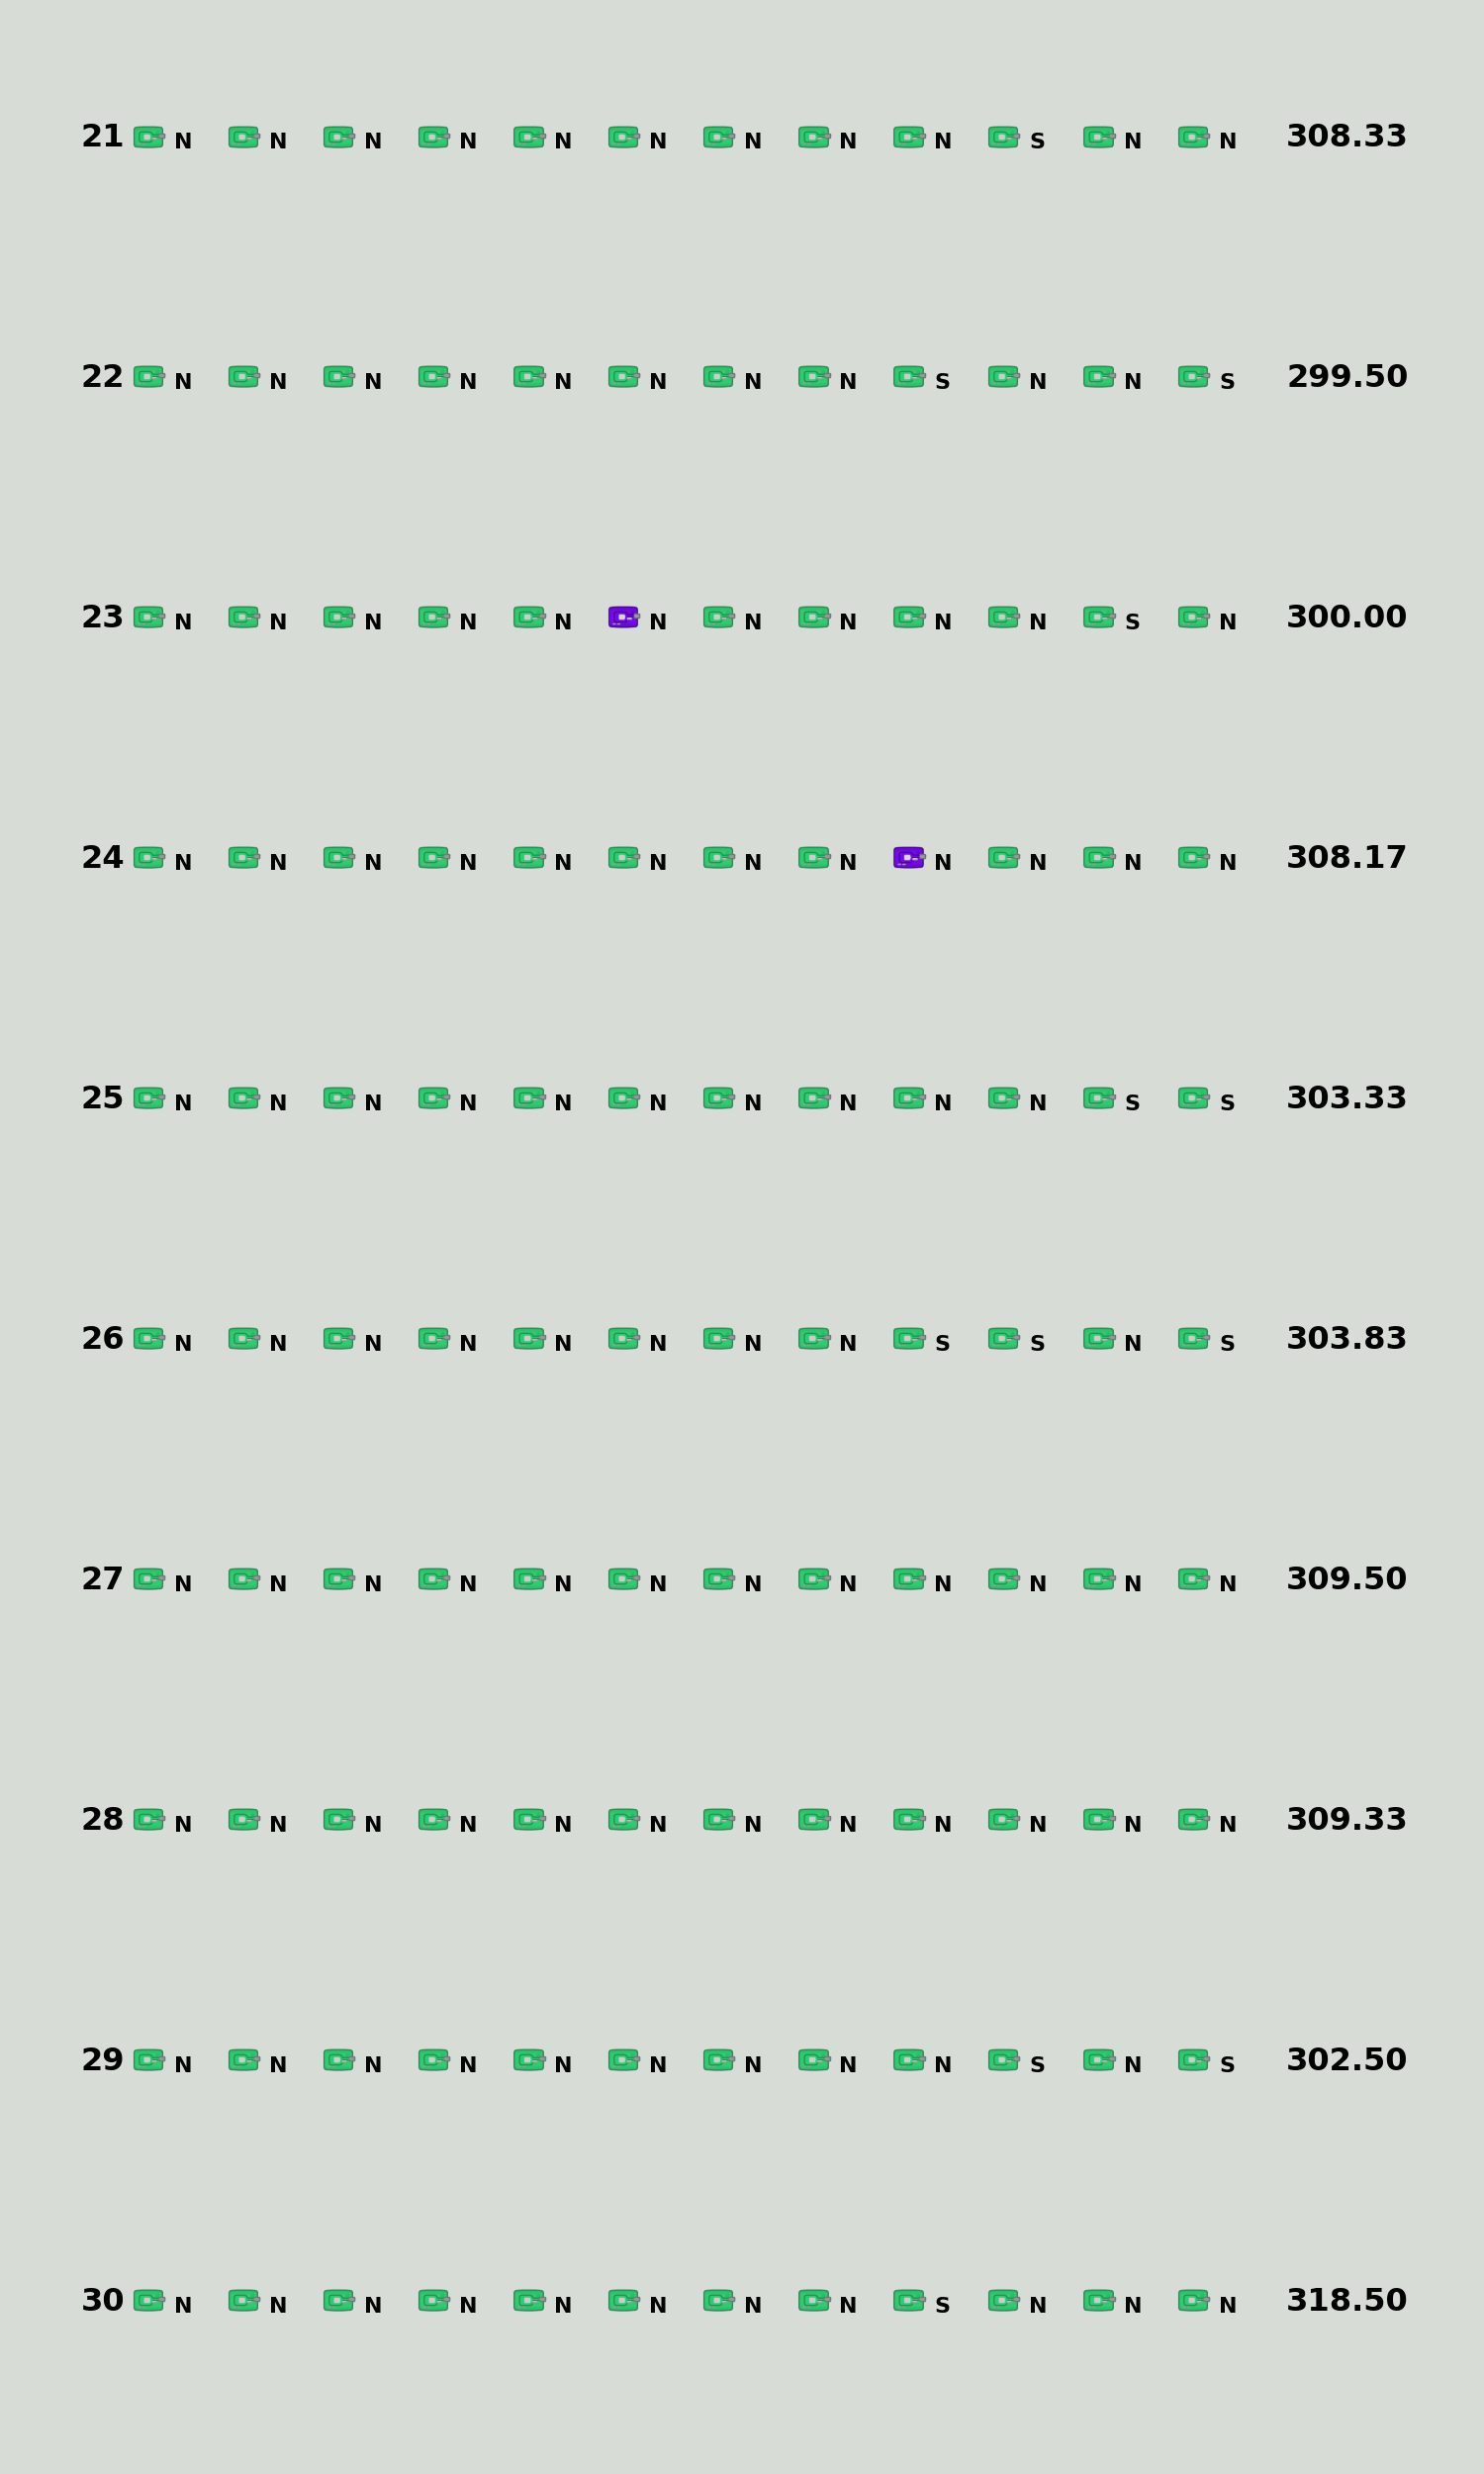
\includegraphics[width=0.9\textwidth]{figuras/td/td_allgreen_ai_mode_1_3.png}
  \caption{Visualização da moda de cada onda com a versão v1 contra Torres Verdes.}
  \label{fig:td-moda-green-1-3}
\end{figure}

%% ------------------------------------------------------------------------- %%
\section{Torres Vermelhas}
\label{sec:apend-moda-td-r-v1}

\begin{figure}[H]
  \centering
  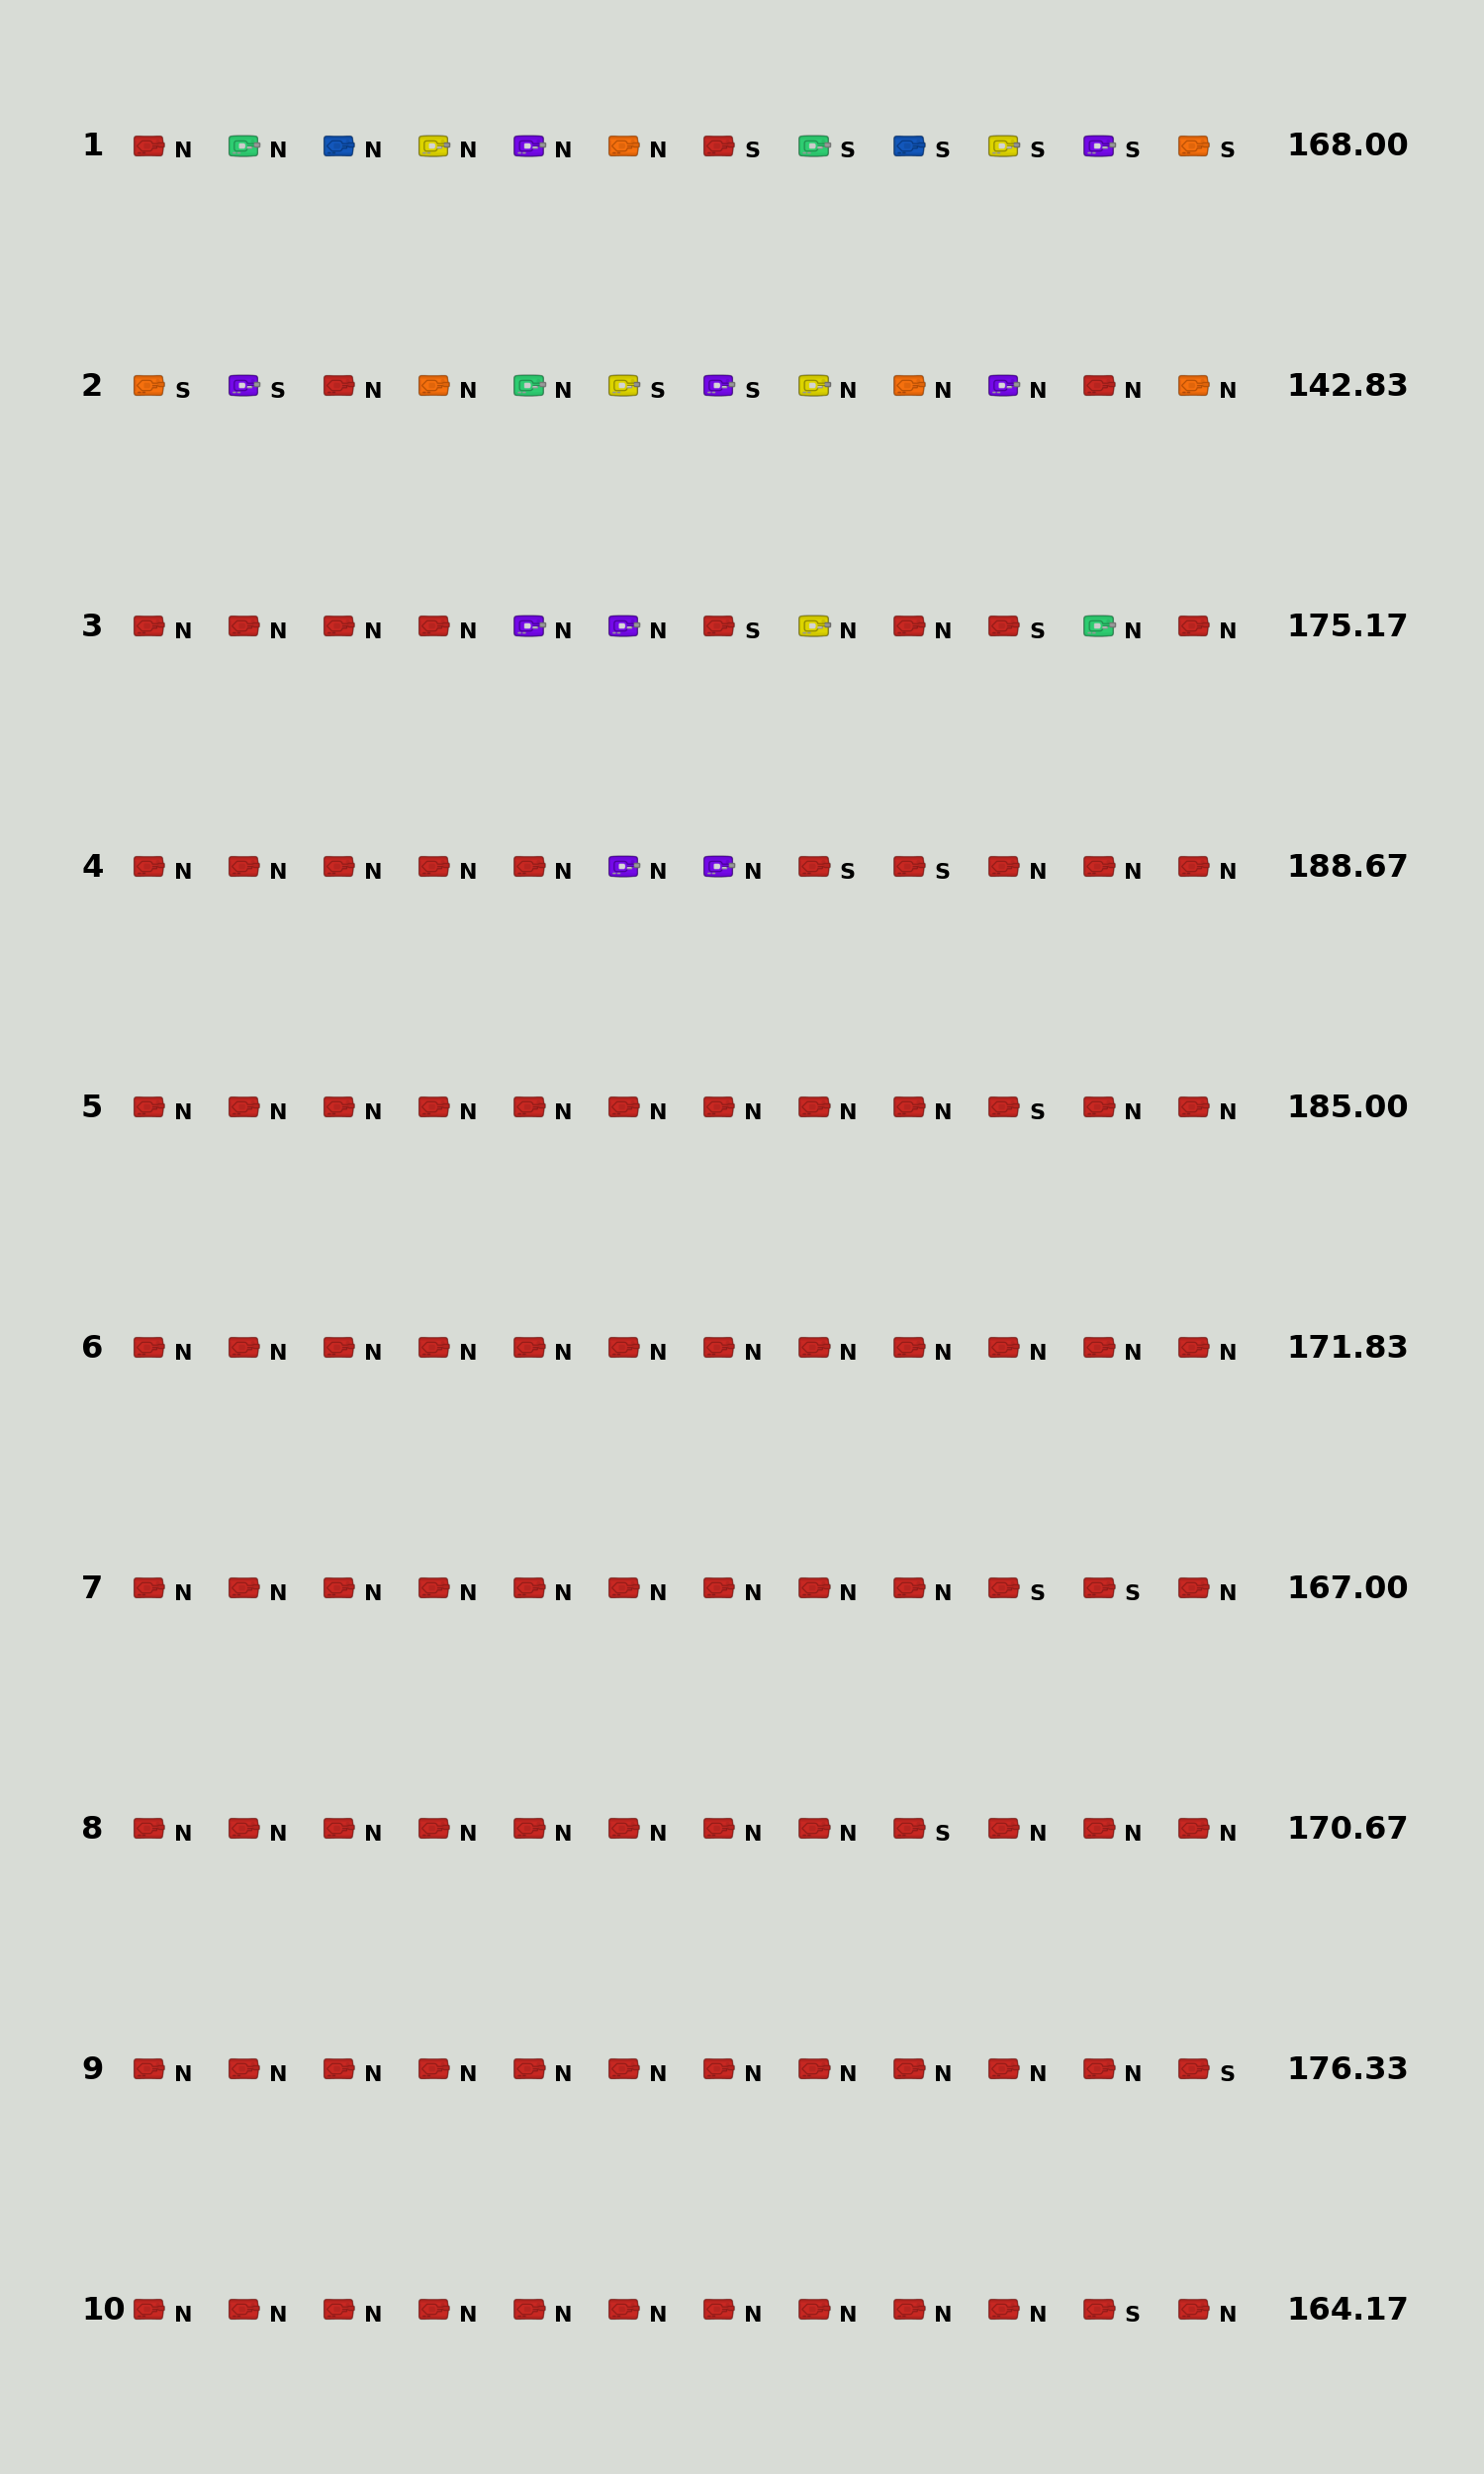
\includegraphics[width=0.9\textwidth]{figuras/td/td_allred_ai_mode_1_1.png}
  \caption{Visualização da moda de cada onda com a versão v1 contra Torres Vermelhas.}
  \label{fig:td-moda-red-1-1}
\end{figure}

\begin{figure}[H]
  \centering
  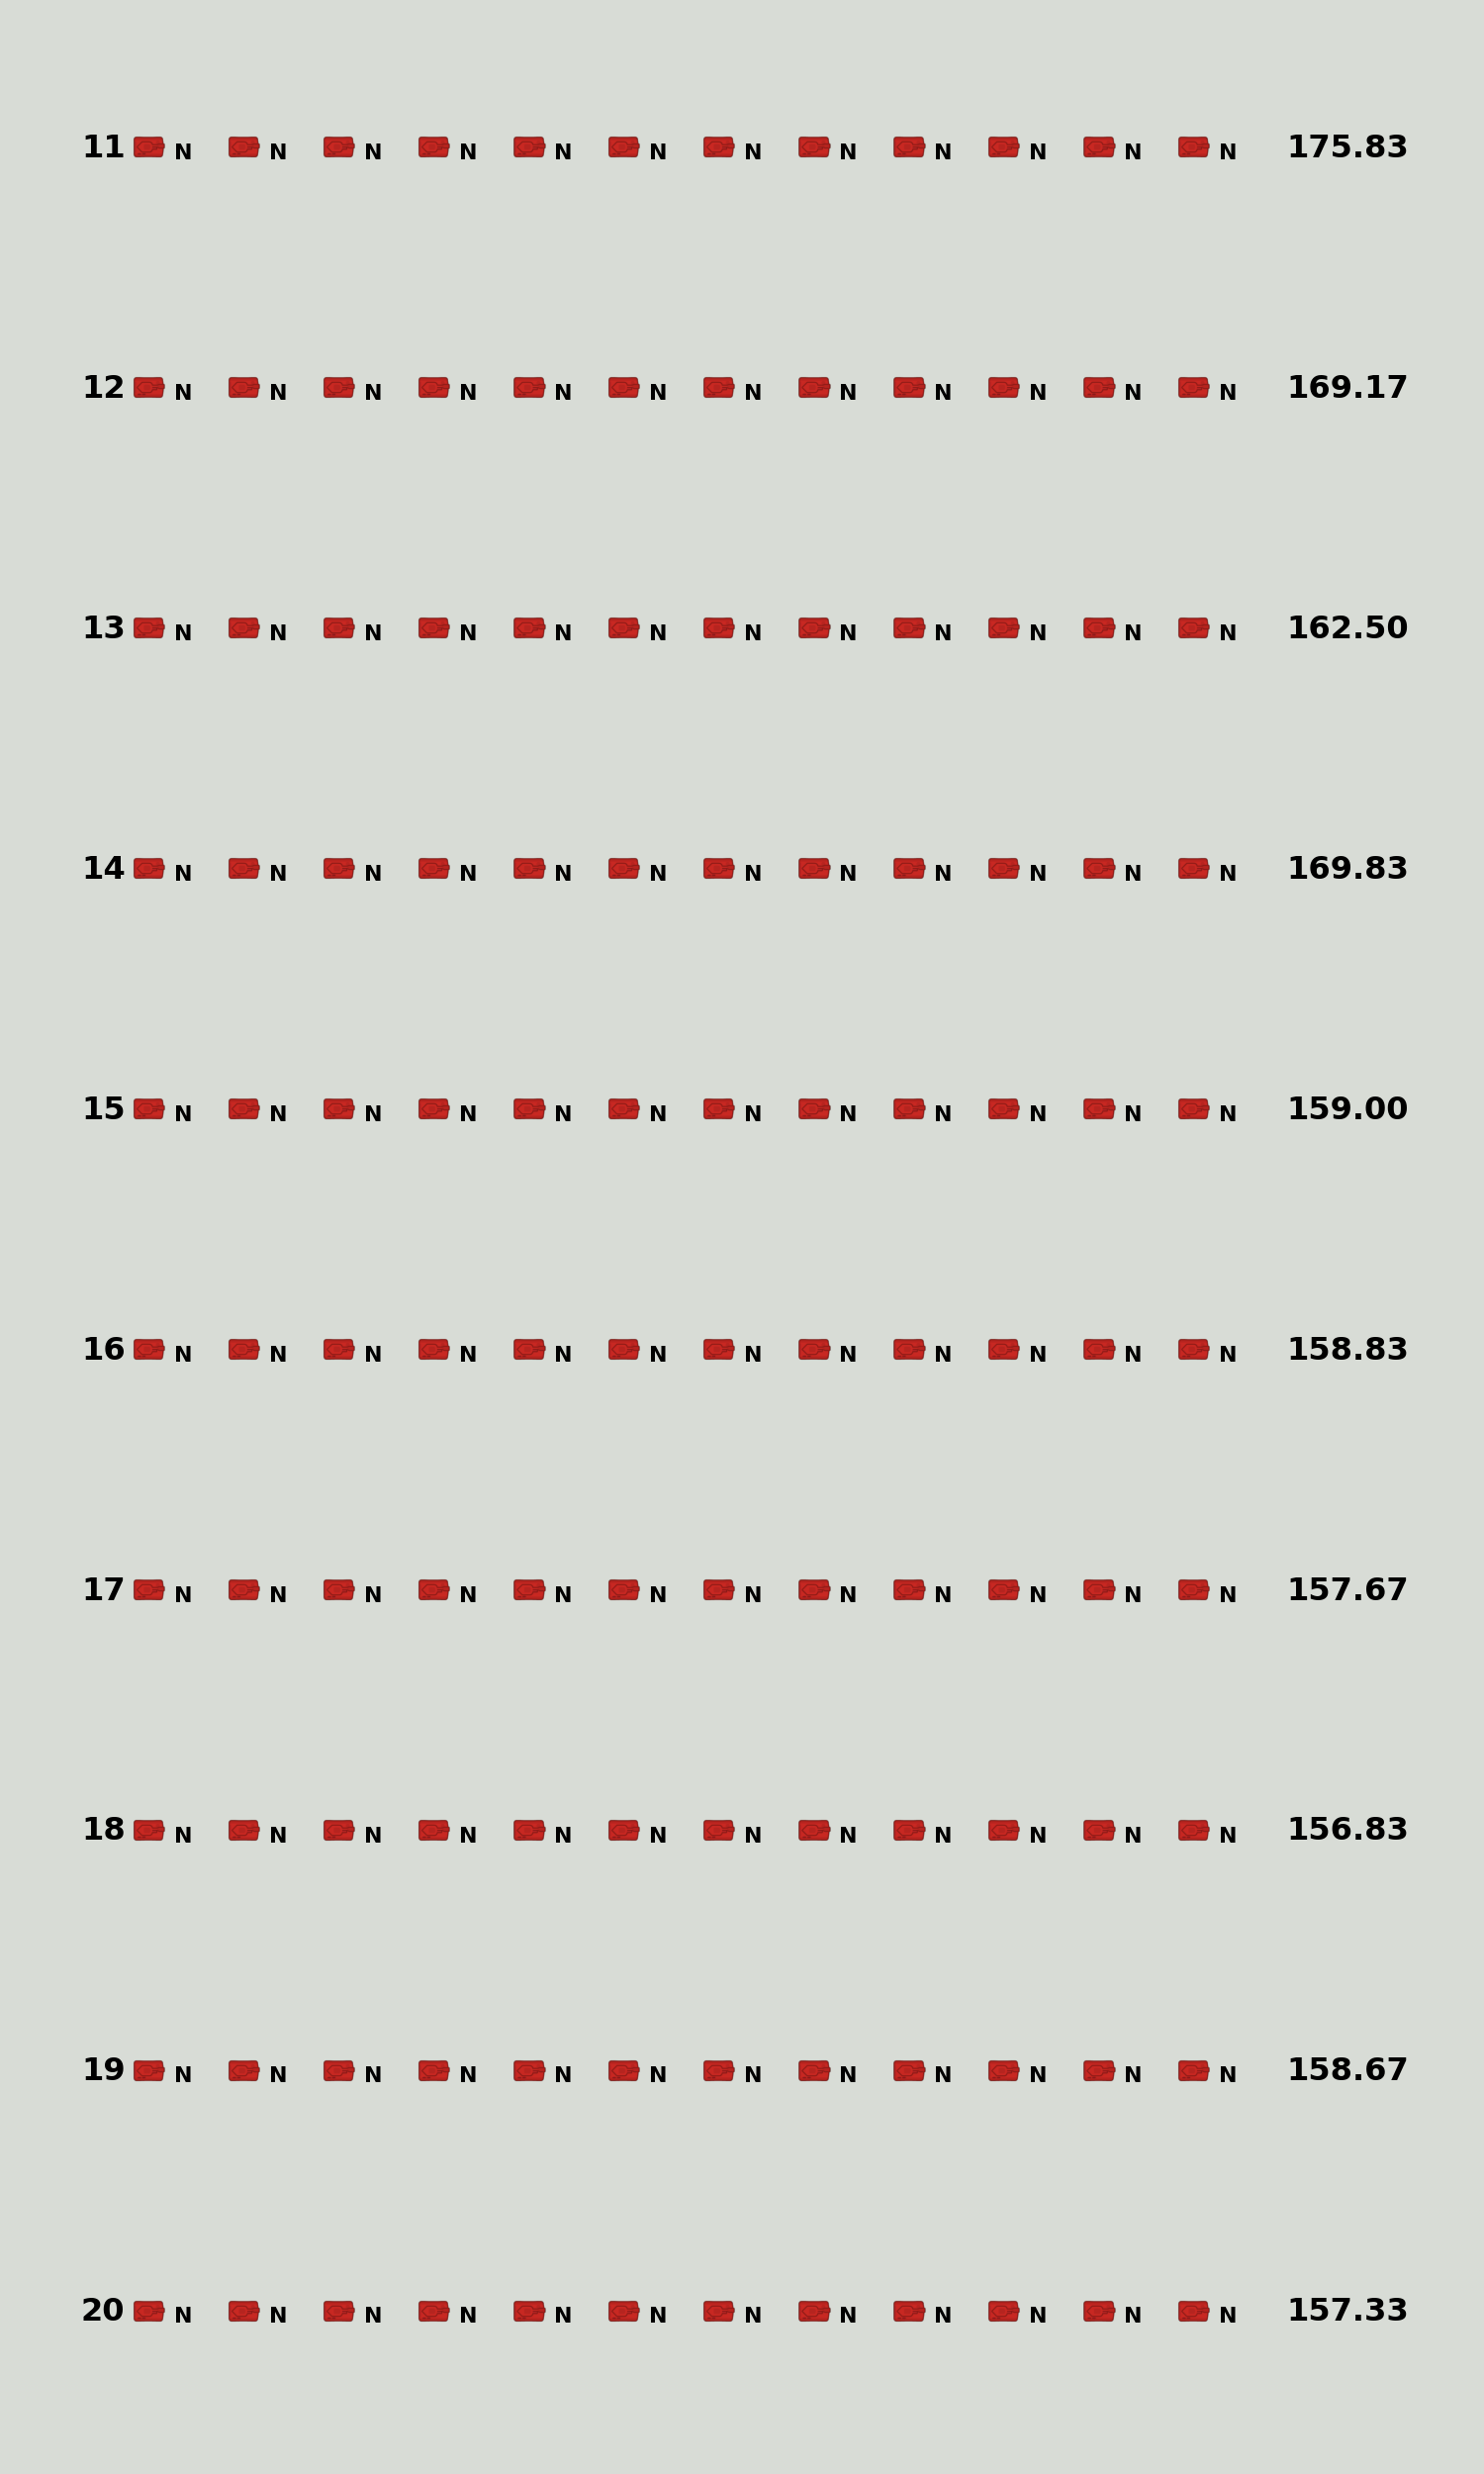
\includegraphics[width=0.9\textwidth]{figuras/td/td_allred_ai_mode_1_2.png}
  \caption{Visualização da moda de cada onda com a versão v1 contra Torres Vermelhas.}
  \label{fig:td-moda-red-1-2}
\end{figure}

\begin{figure}[H]
  \centering
  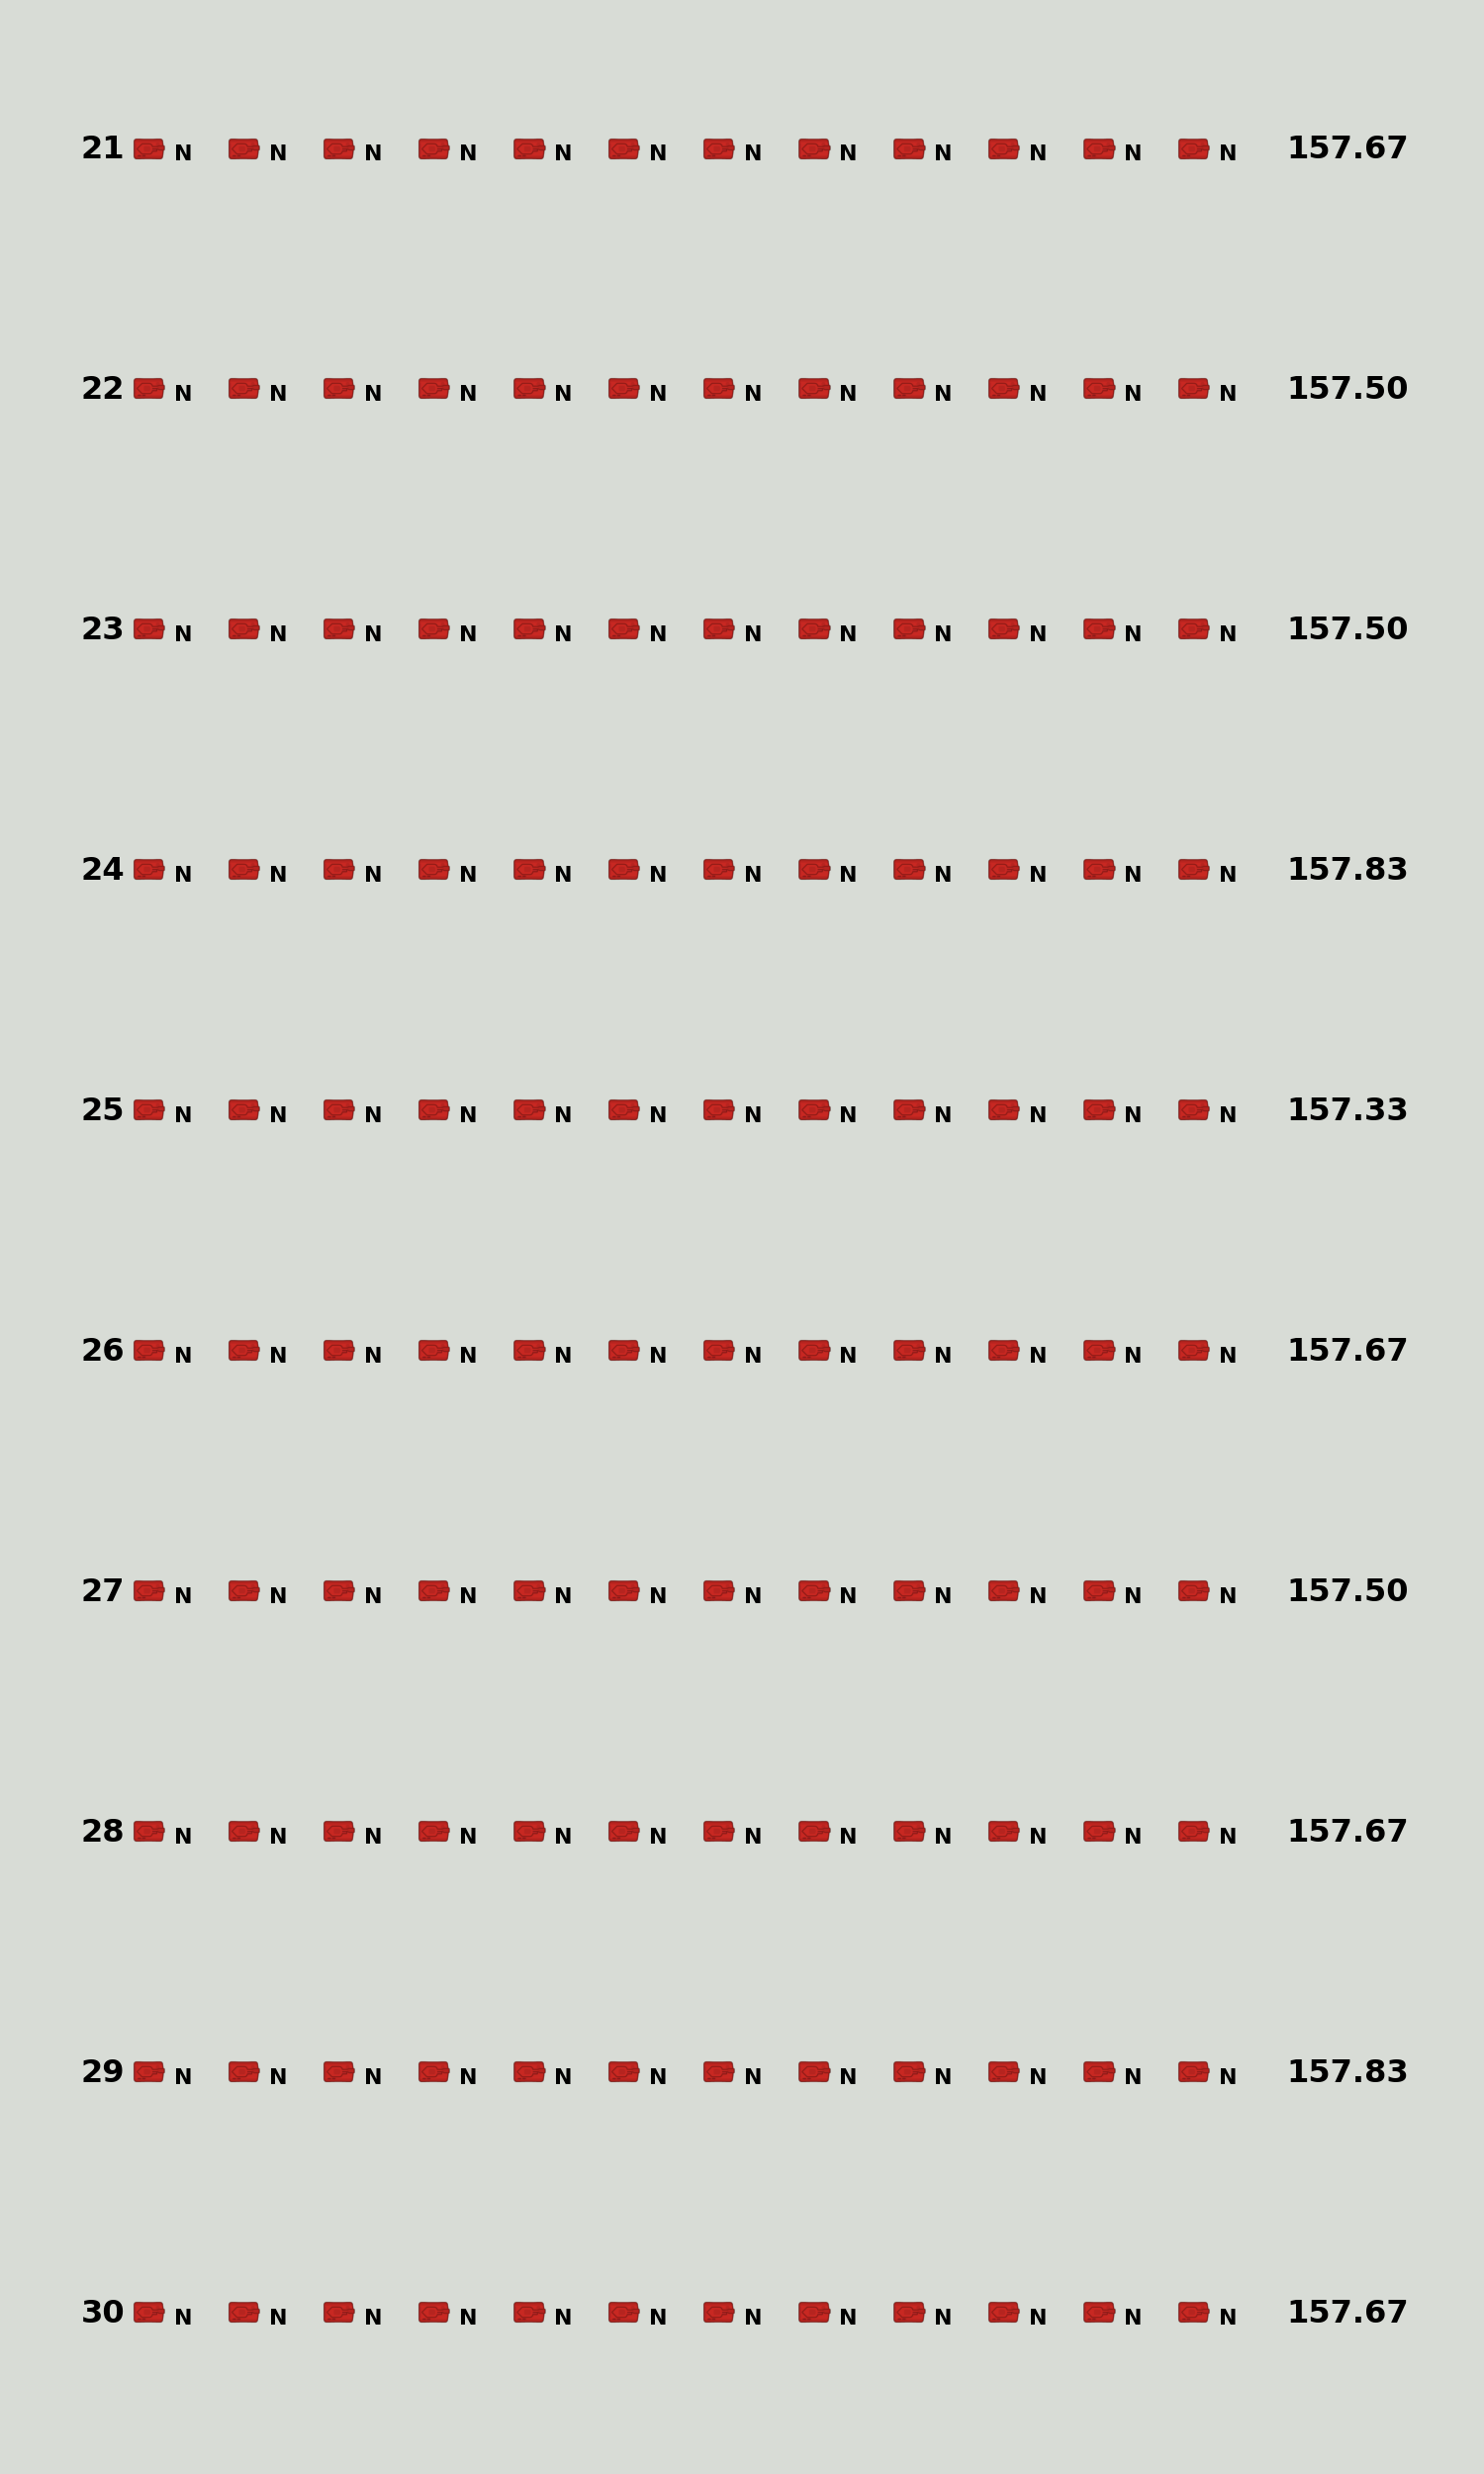
\includegraphics[width=0.9\textwidth]{figuras/td/td_allred_ai_mode_1_3.png}
  \caption{Visualização da moda de cada onda com a versão v1 contra Torres Vermelhas.}
  \label{fig:td-moda-red-1-3}
\end{figure}

%% ------------------------------------------------------------------------- %%
\section{Torres Verde + Vermelha}
\label{sec:apend-moda-td-gr-v1}

\begin{figure}[H]
  \centering
  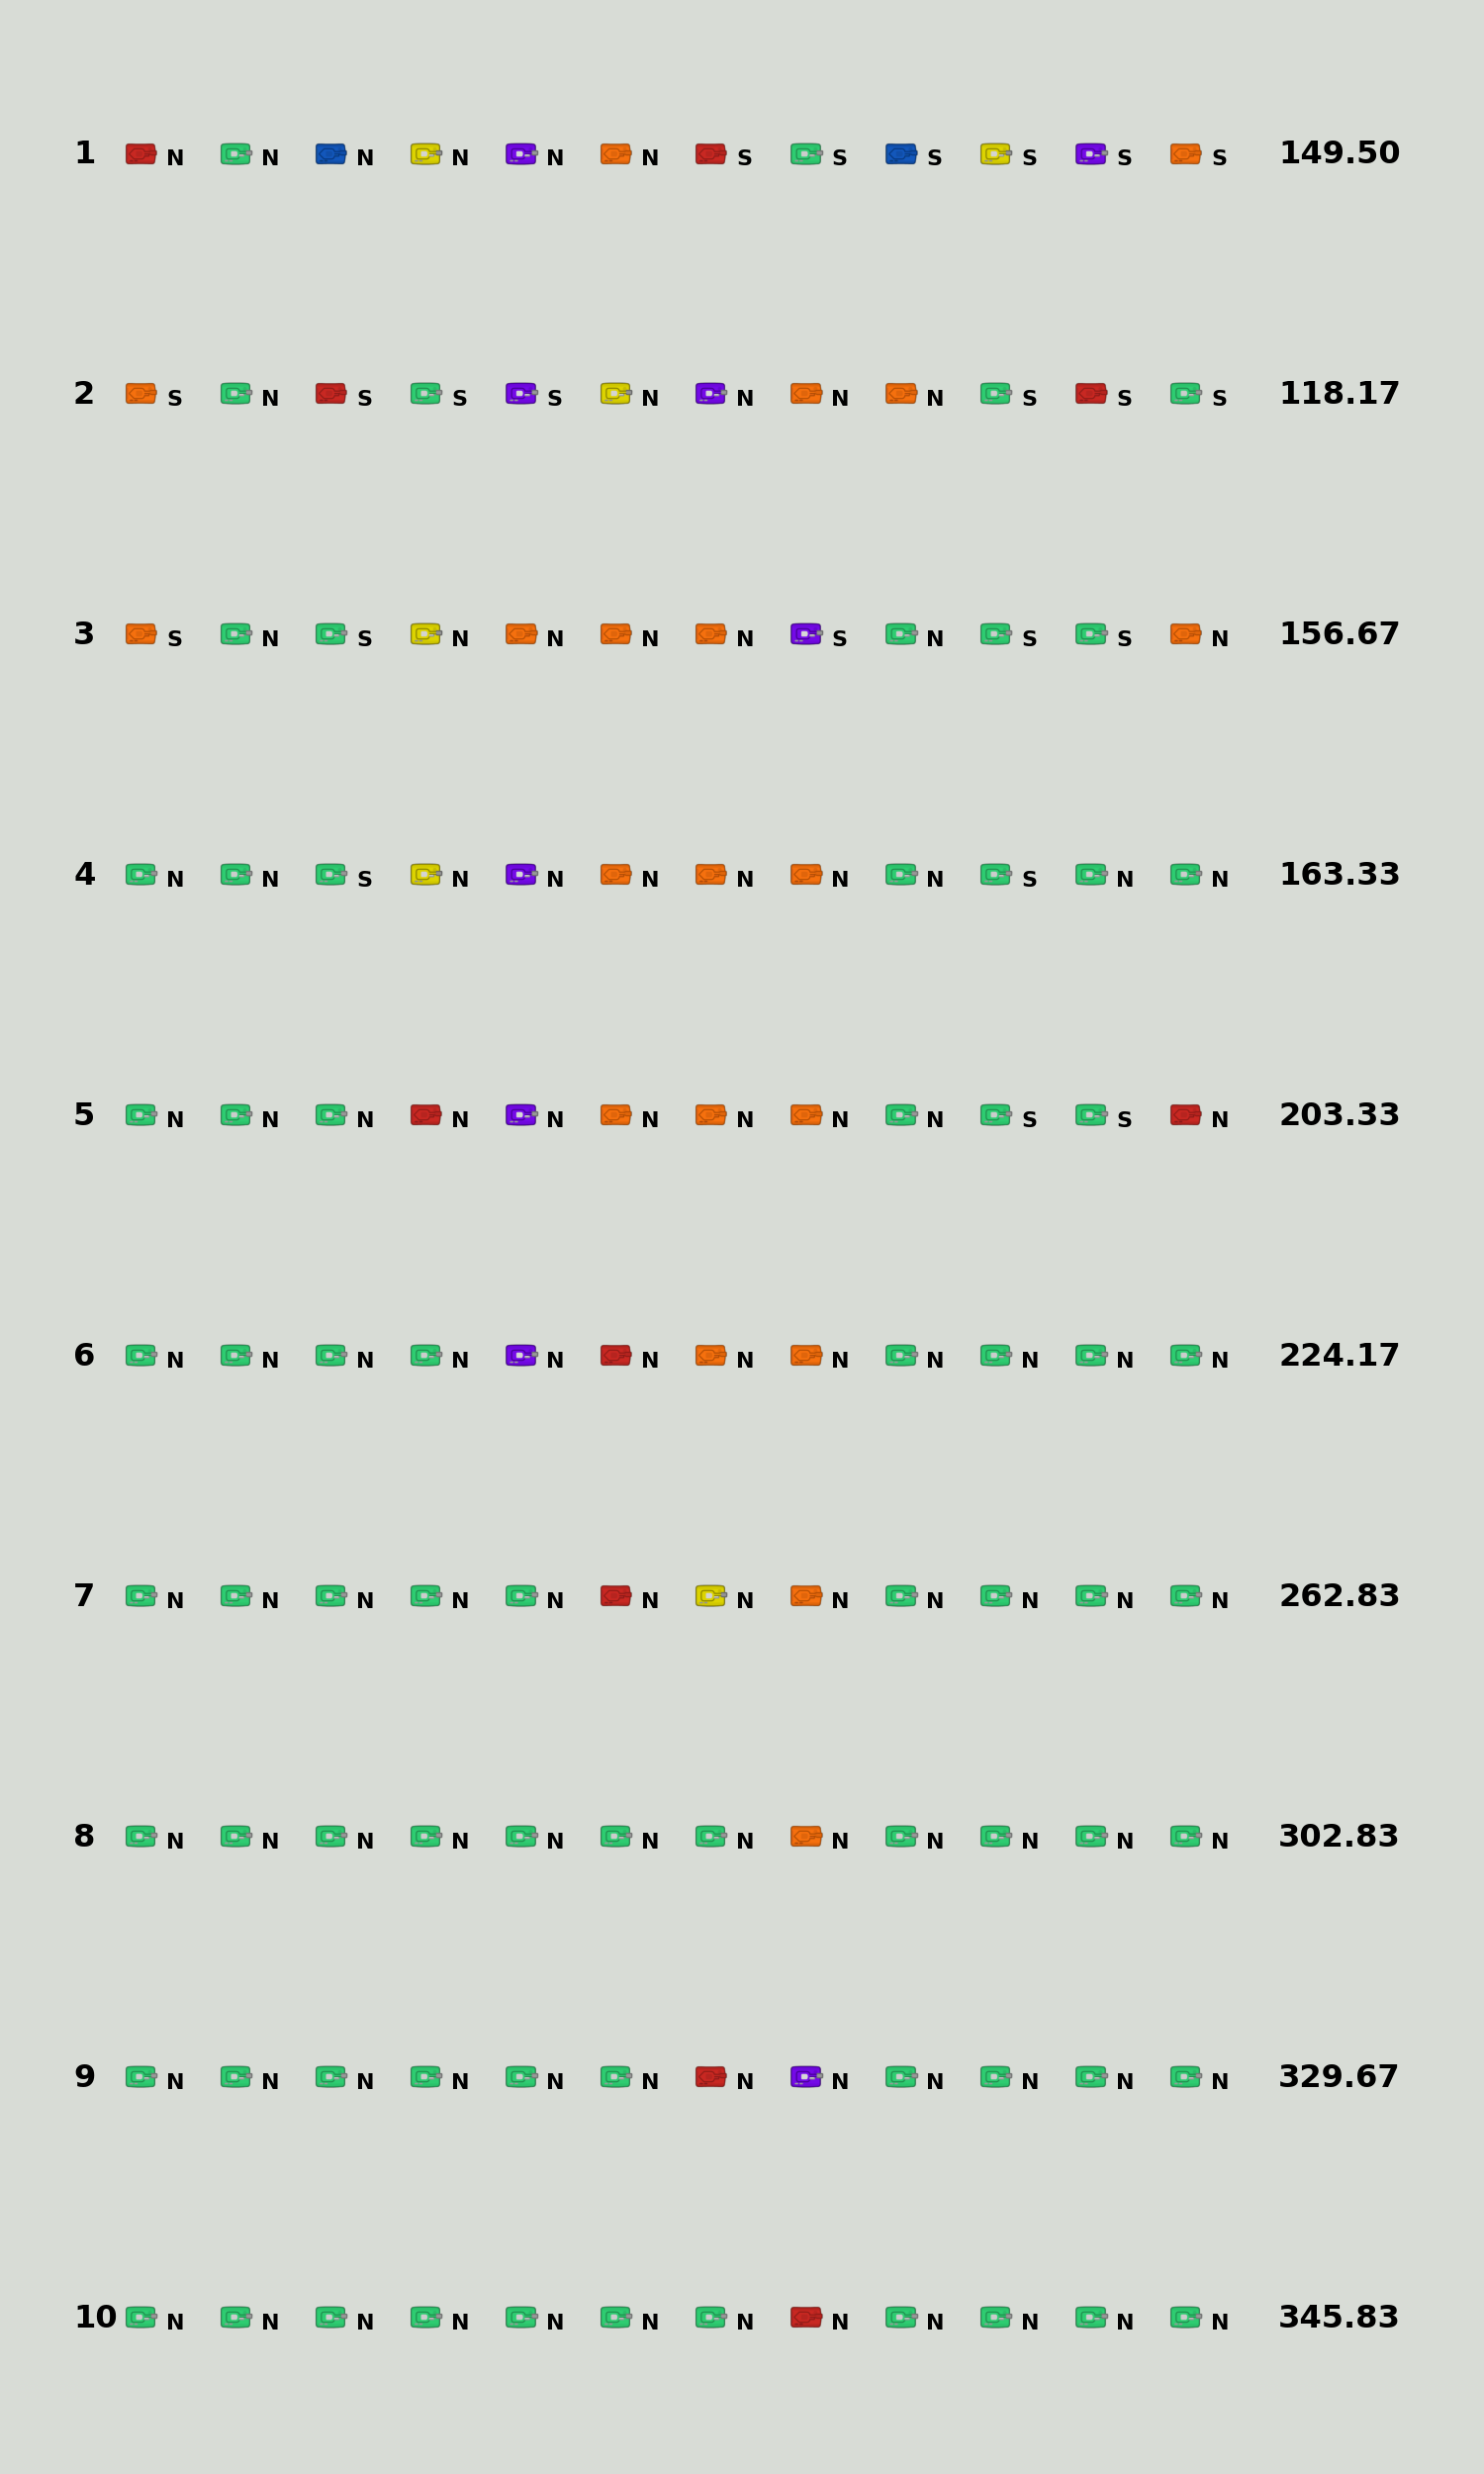
\includegraphics[width=0.9\textwidth]{figuras/td/td_greenred_ai_mode_1_1.png}
  \caption{Visualização da moda de cada onda com a versão v1 contra Torres Verdes + Vermelhas.}
  \label{fig:td-moda-greenred-1-1}
\end{figure}

\begin{figure}[H]
  \centering
  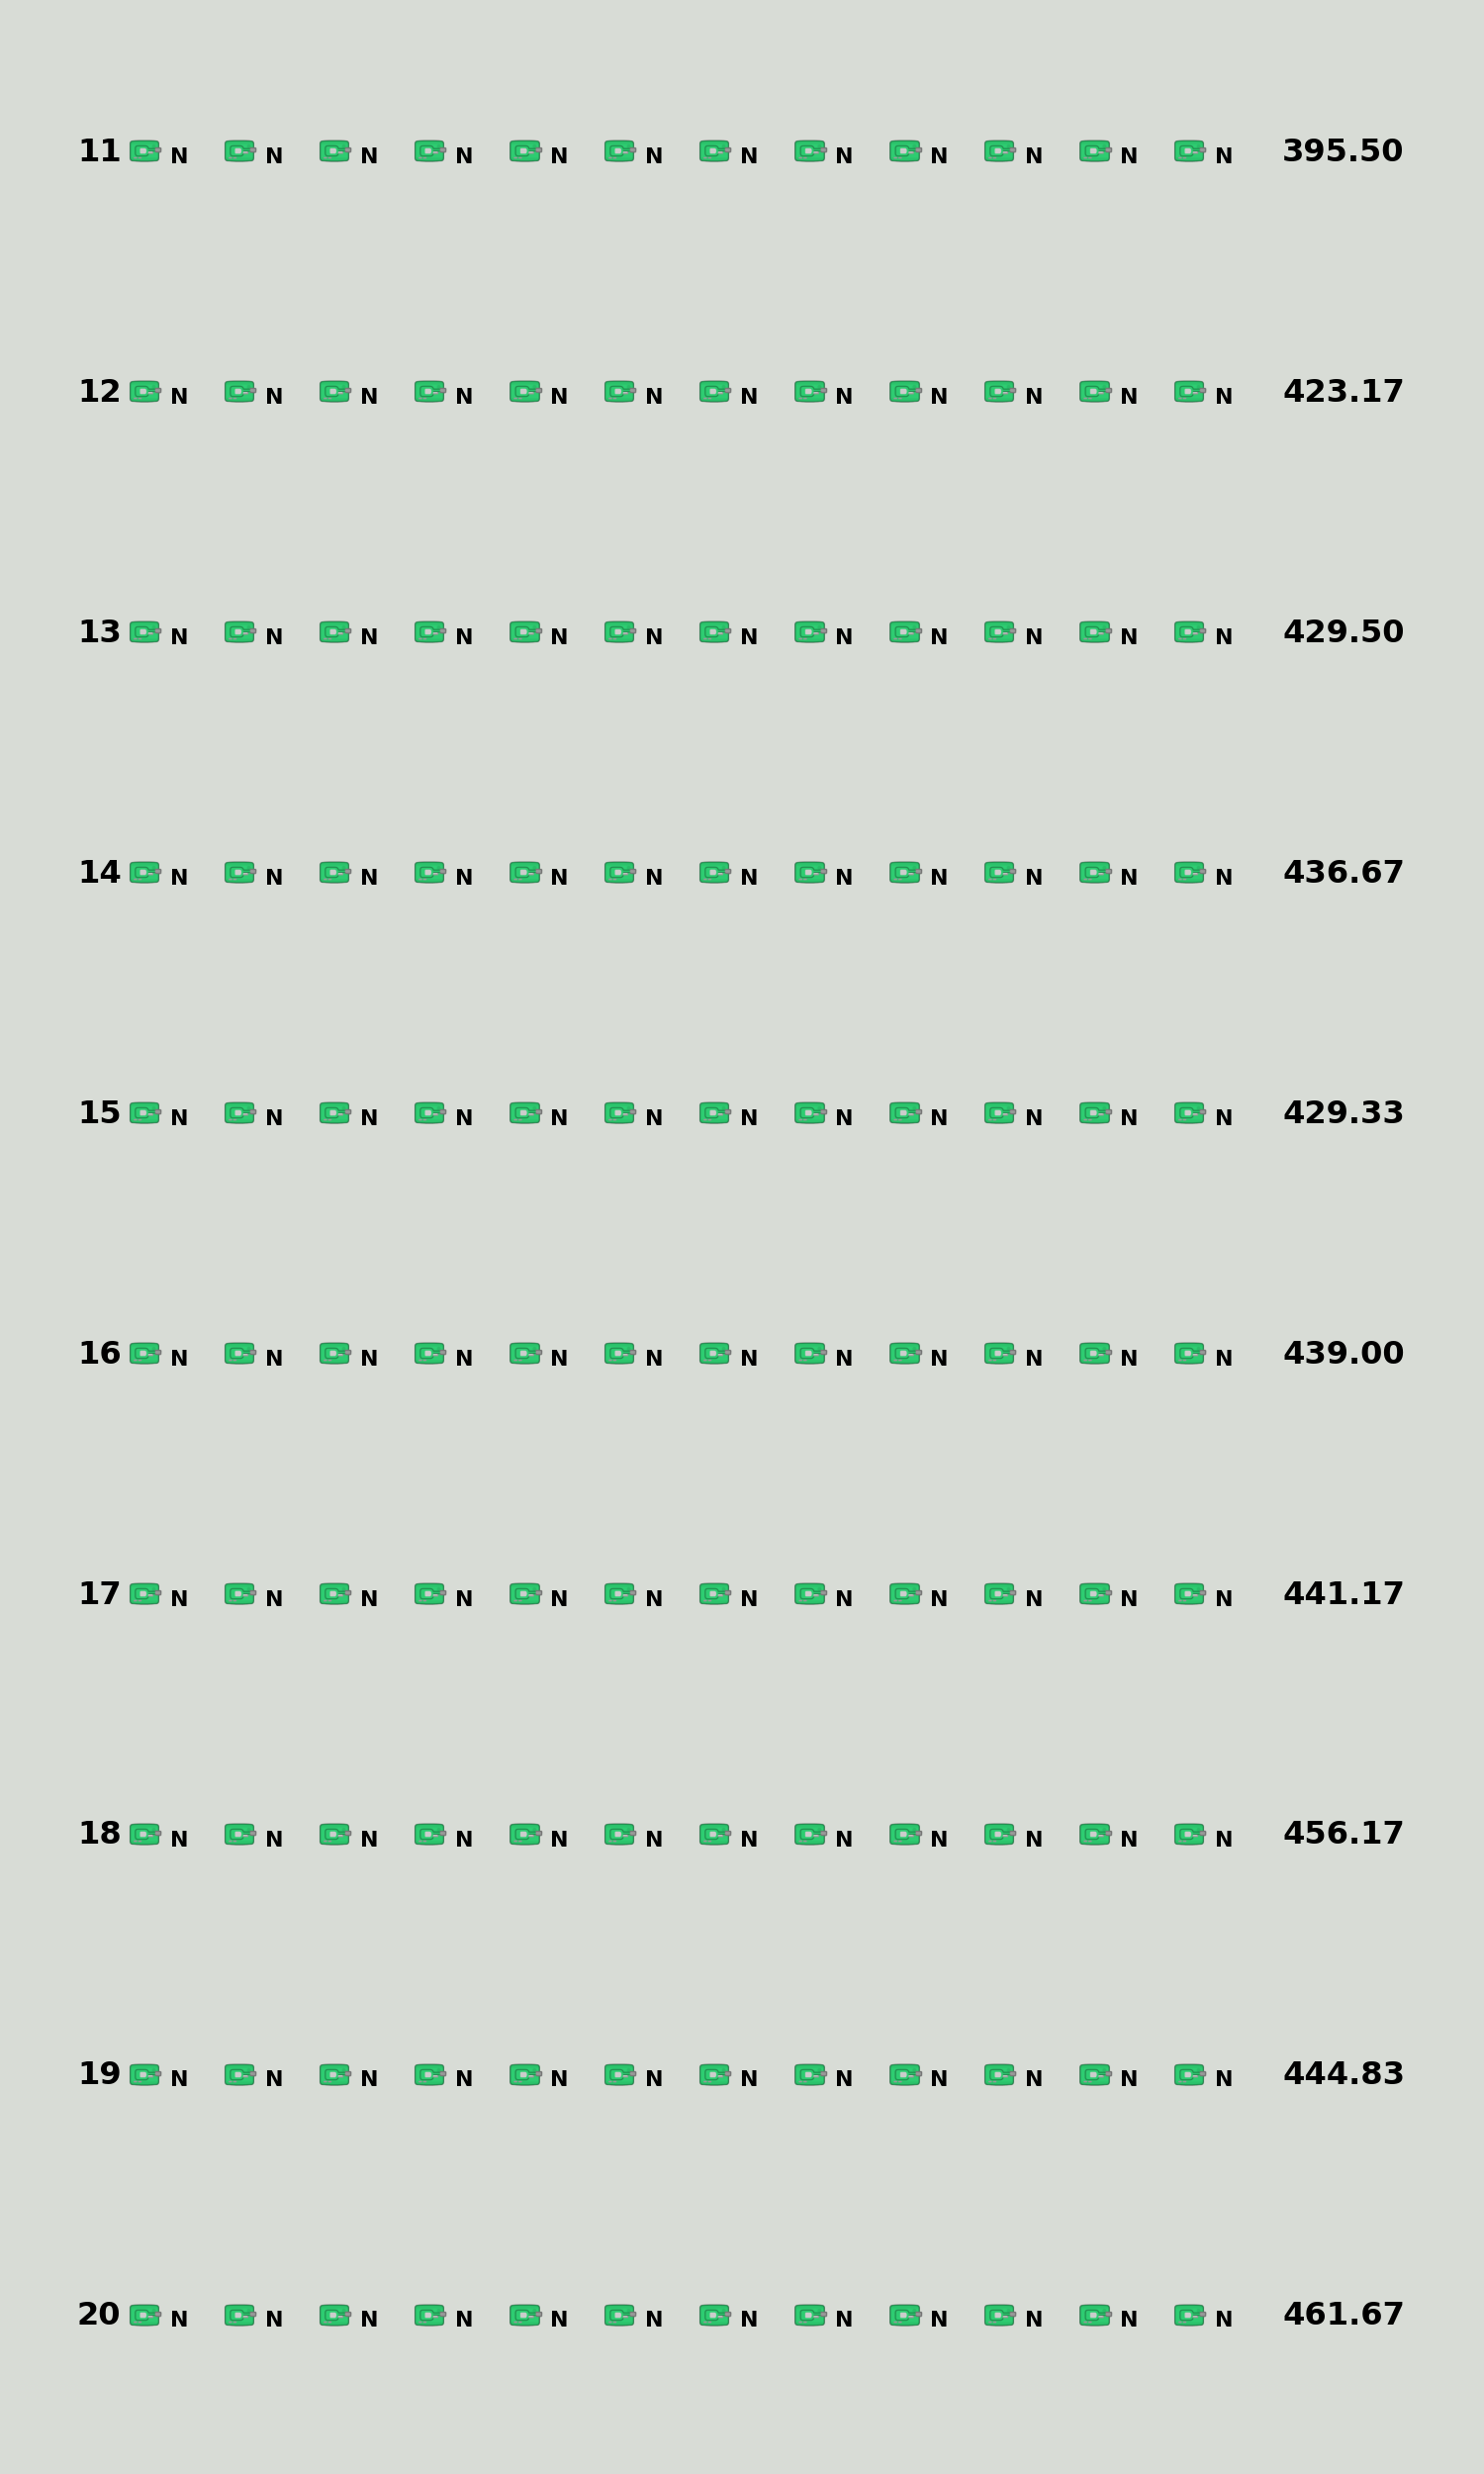
\includegraphics[width=0.9\textwidth]{figuras/td/td_greenred_ai_mode_1_2.png}
  \caption{Visualização da moda de cada onda com a versão v1 contra Torres Verdes + Vermelhas.}
  \label{fig:td-moda-greenred-1-2}
\end{figure}

\begin{figure}[H]
  \centering
  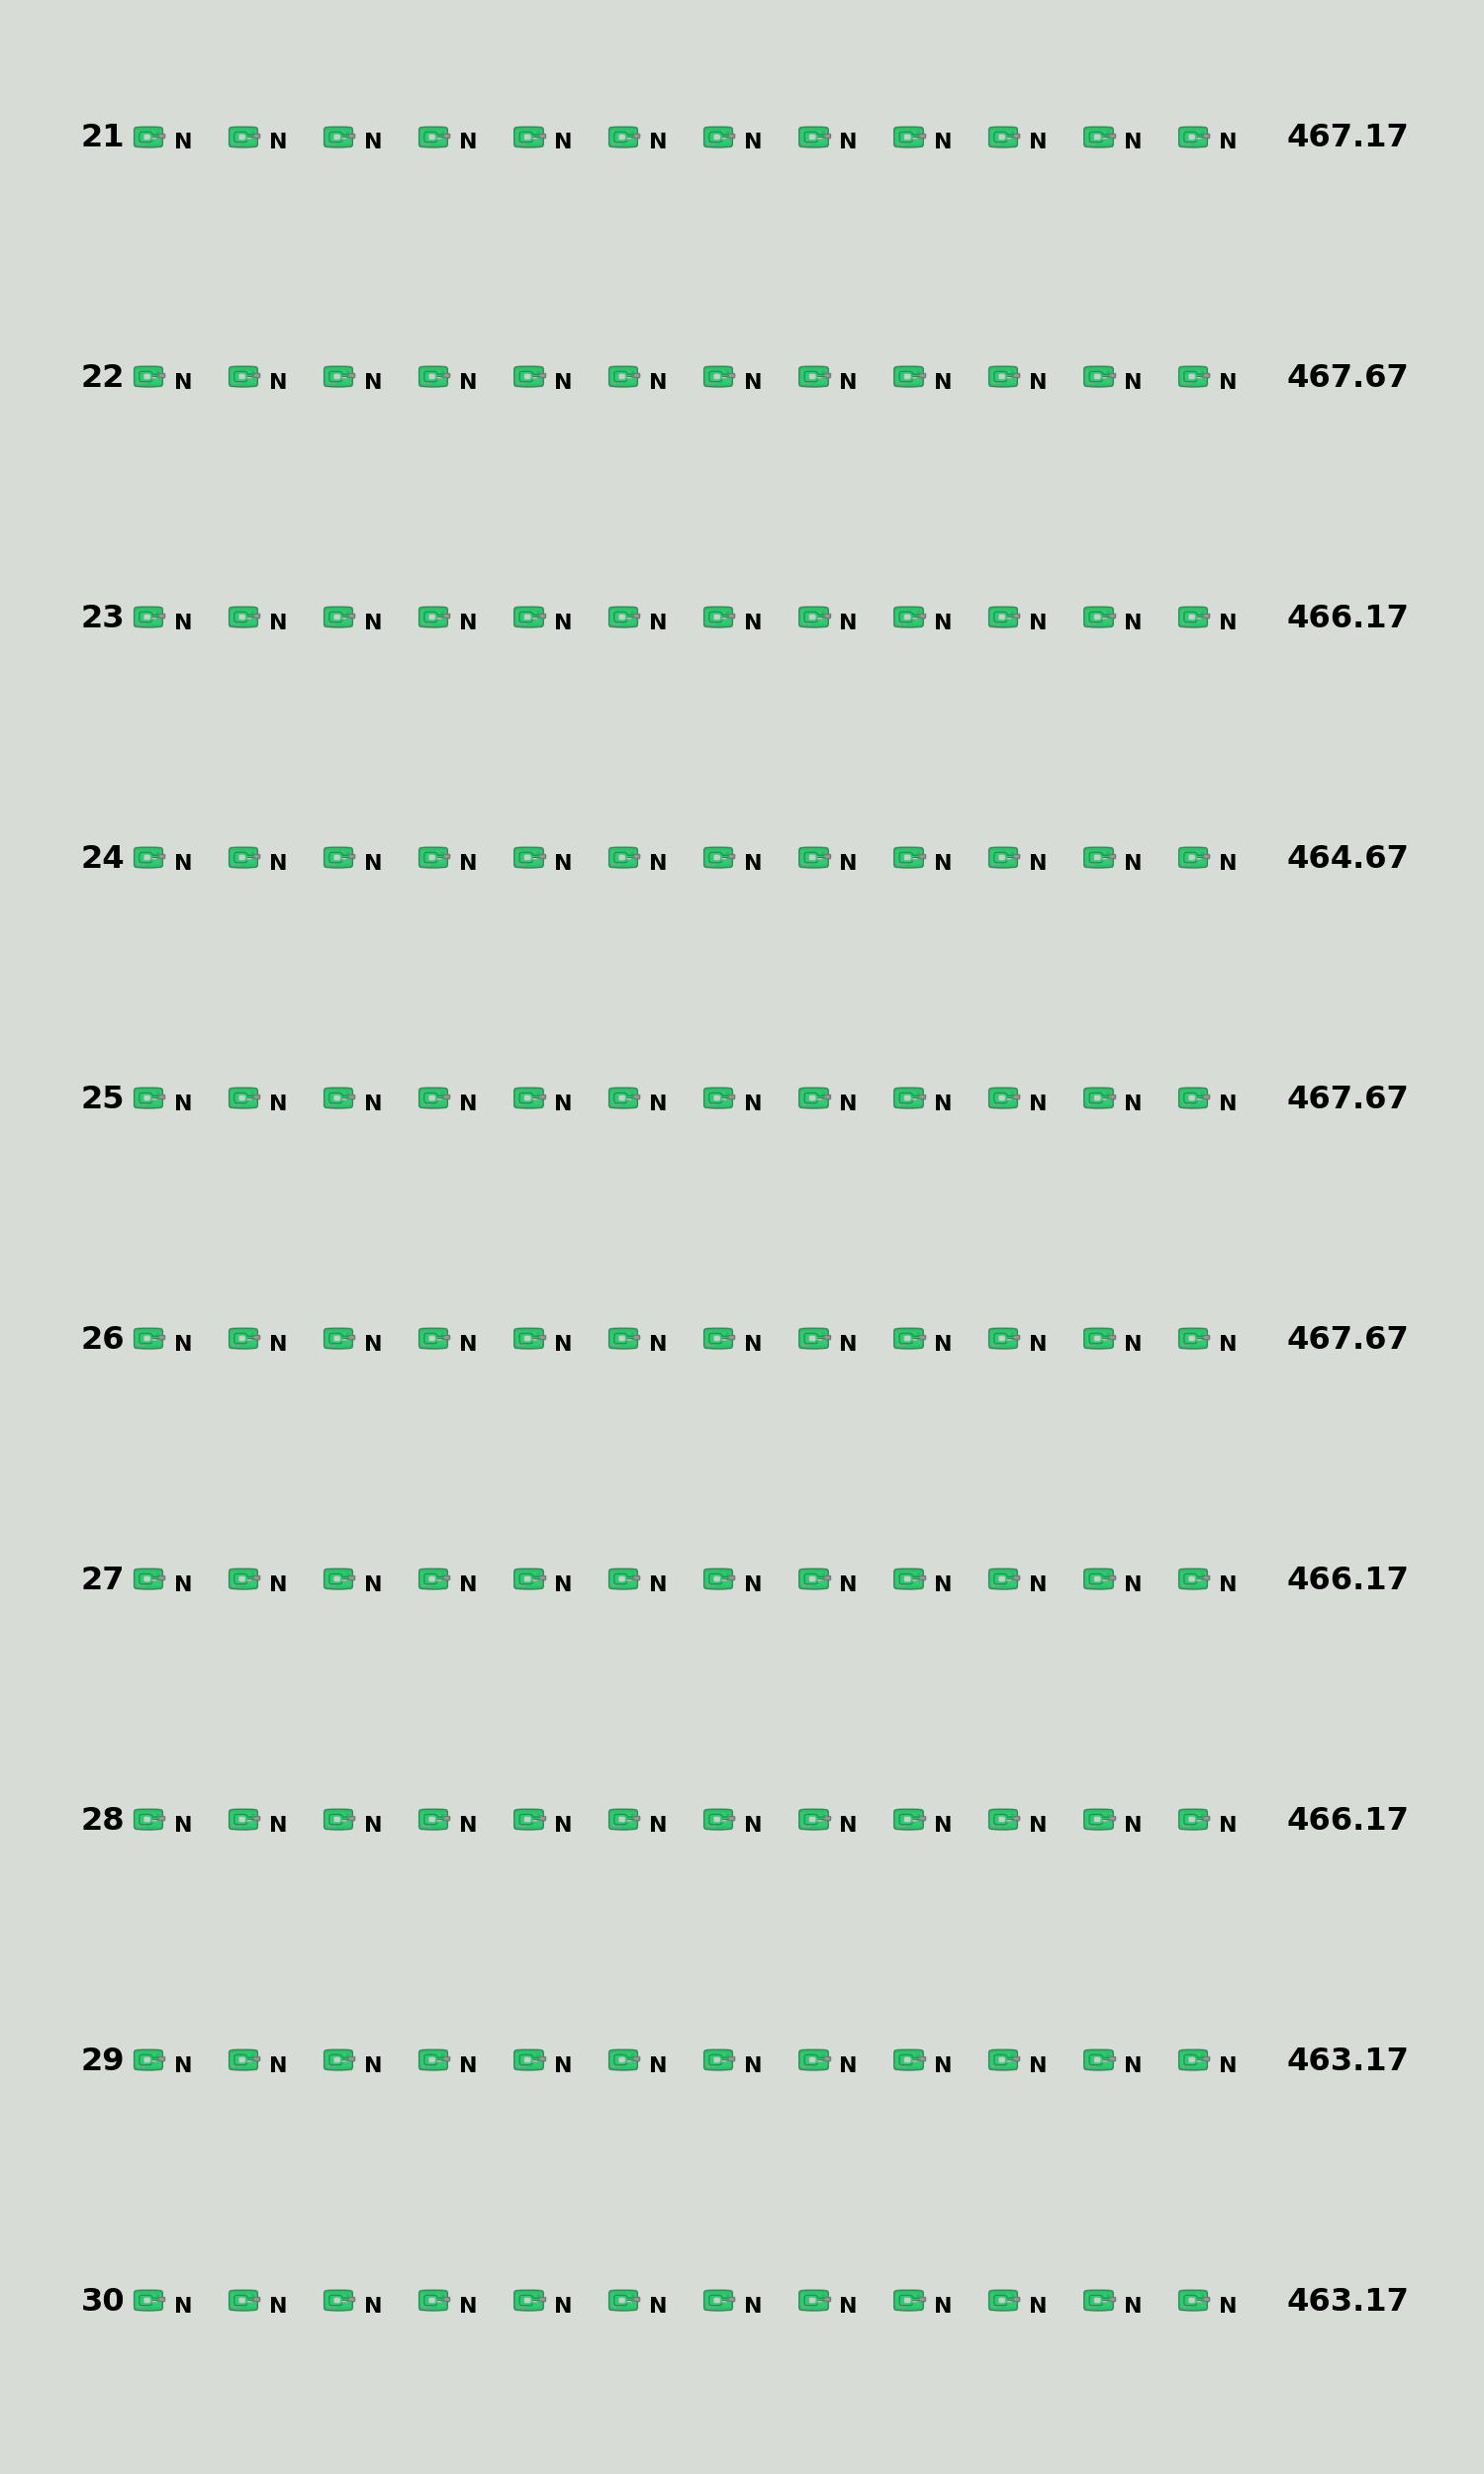
\includegraphics[width=0.9\textwidth]{figuras/td/td_greenred_ai_mode_1_3.png}
  \caption{Visualização da moda de cada onda com a versão v1 contra Torres Verdes + Vermelhas.}
  \label{fig:td-moda-greenred-1-3}
\end{figure}

%% ------------------------------------------------------------------------- %%
\section{Torres Vermelha + Verde}
\label{sec:apend-moda-td-rg-v1}

\begin{figure}[H]
  \centering
  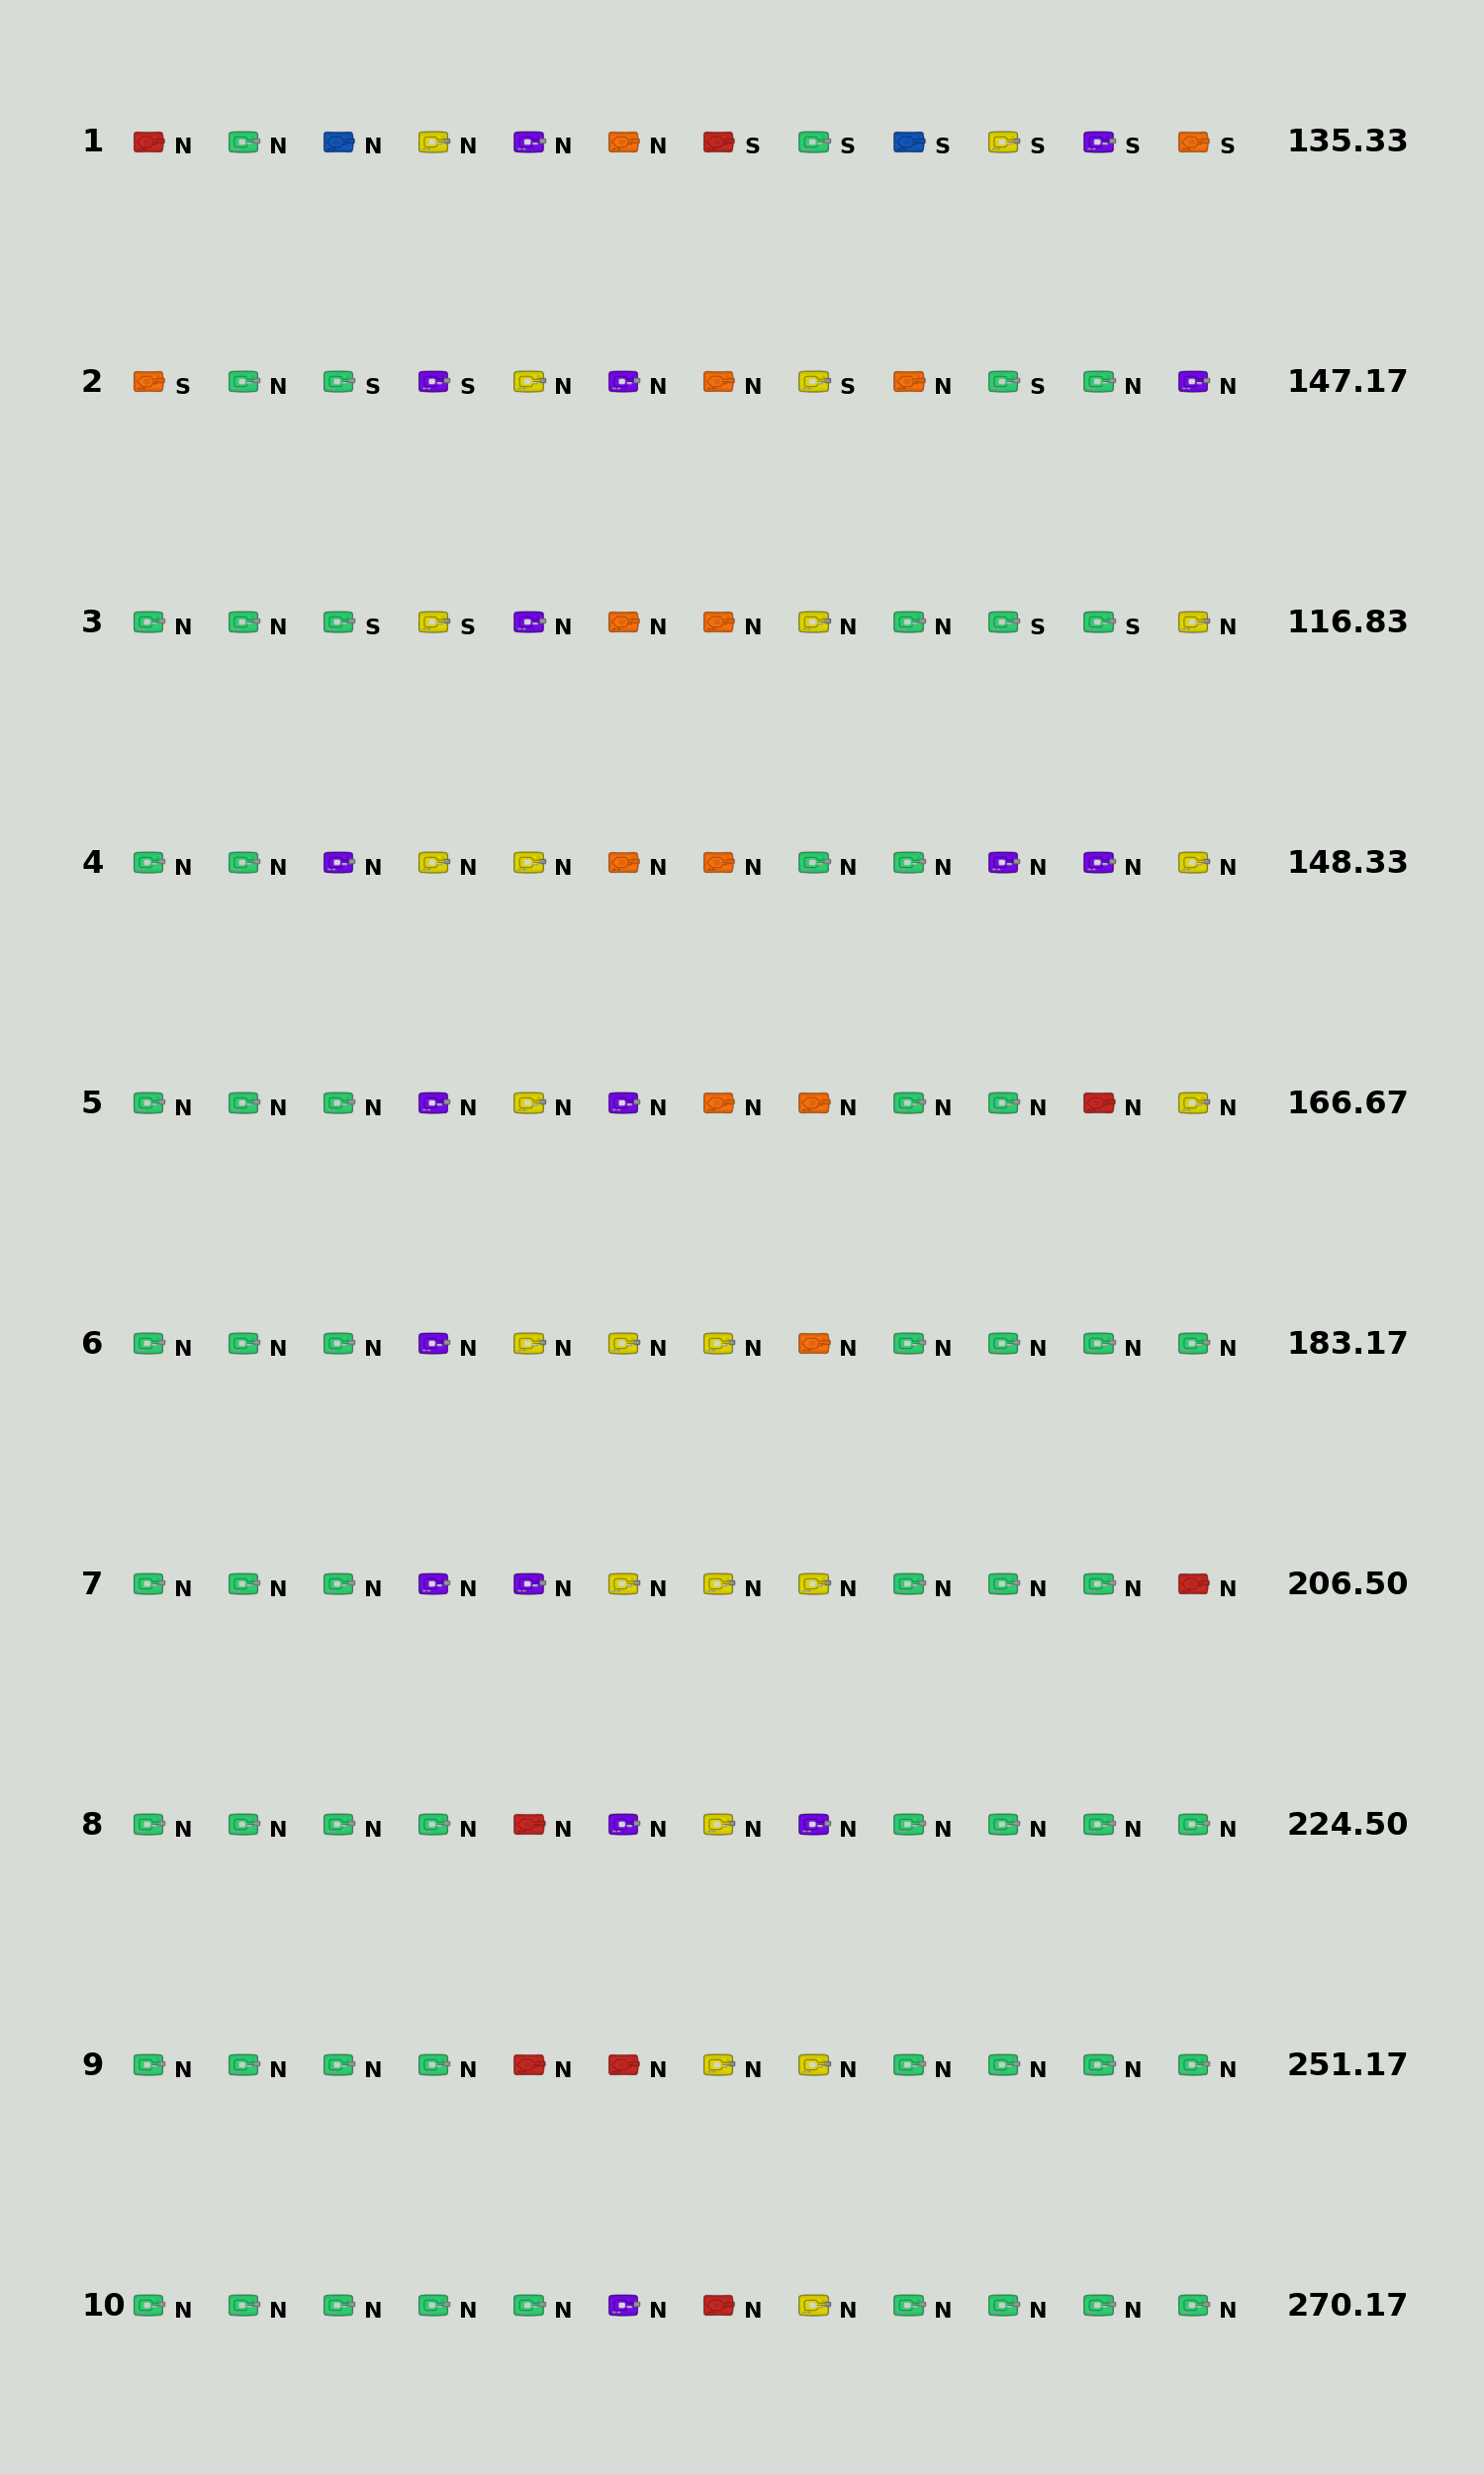
\includegraphics[width=0.9\textwidth]{figuras/td/td_redgreen_ai_mode_1_1.png}
  \caption{Visualização da moda de cada onda com a versão v1 contra Torres Vermelhas + Verdes.}
  \label{fig:td-moda-redgreen-1-1}
\end{figure}

\begin{figure}[H]
  \centering
  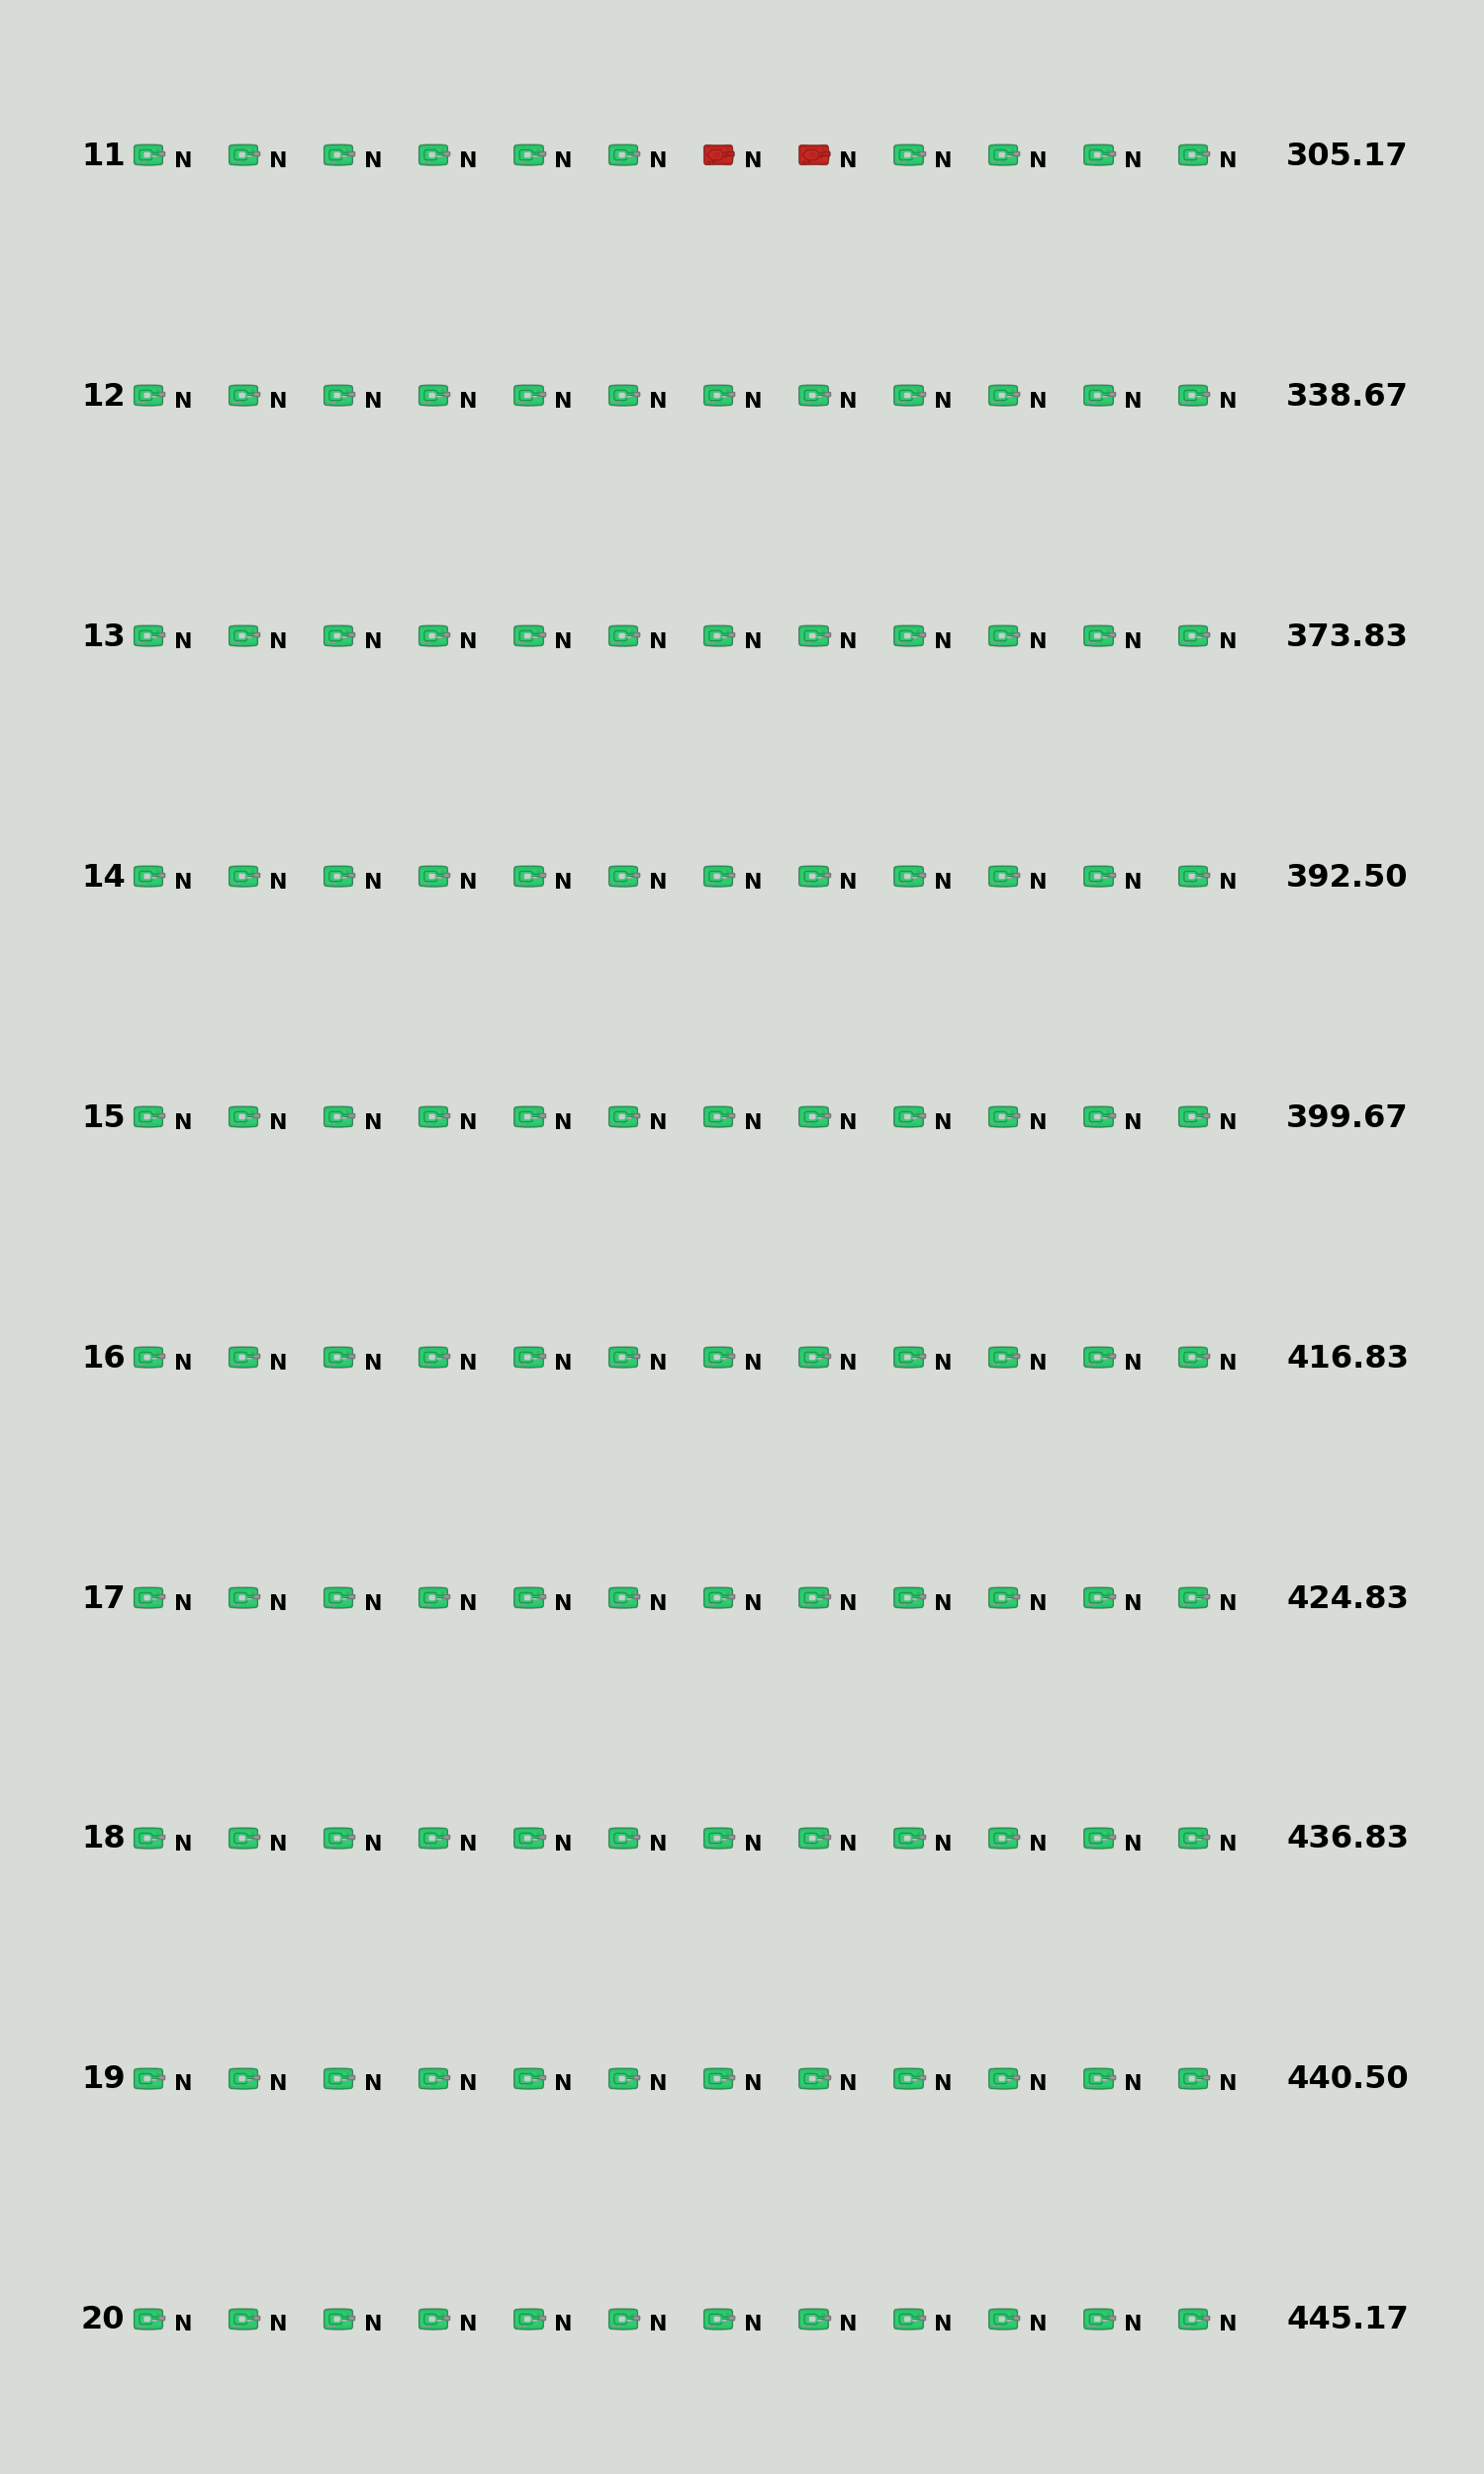
\includegraphics[width=0.9\textwidth]{figuras/td/td_redgreen_ai_mode_1_2.png}
  \caption{Visualização da moda de cada onda com a versão v1 contra Torres Vermelhas + Verdes.}
  \label{fig:td-moda-redgreen-1-2}
\end{figure}

\begin{figure}[H]
  \centering
  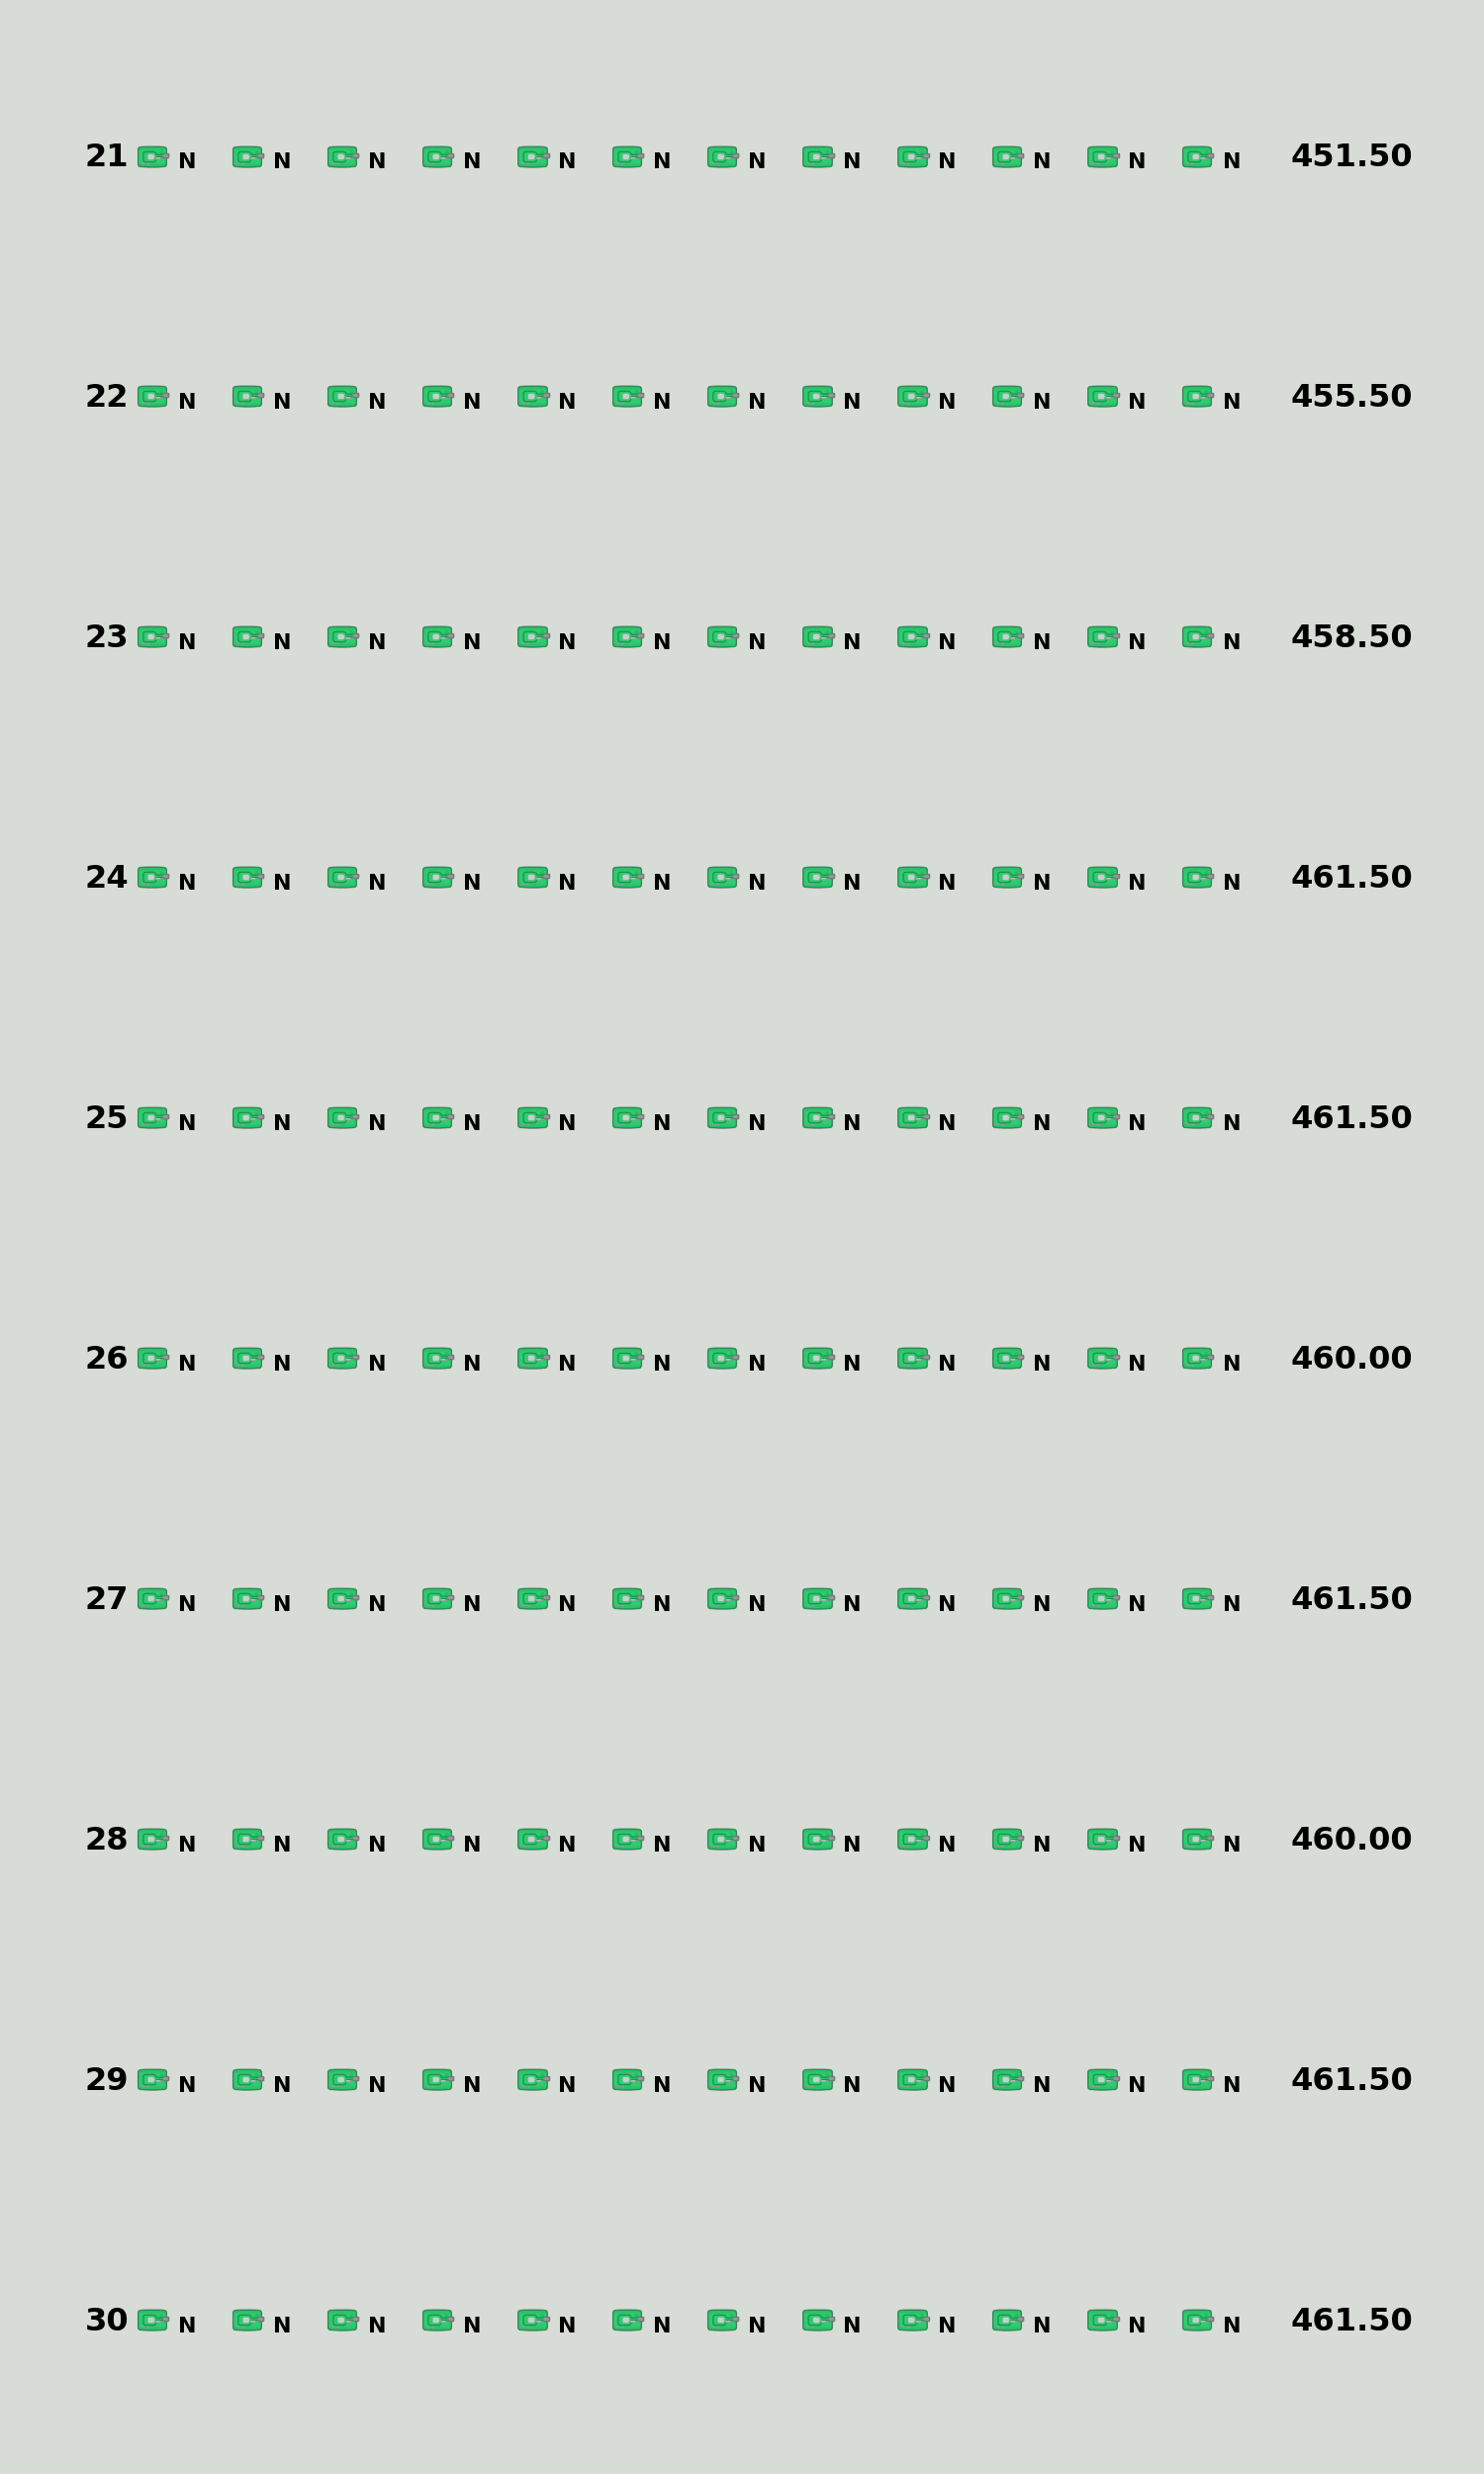
\includegraphics[width=0.9\textwidth]{figuras/td/td_redgreen_ai_mode_1_3.png}
  \caption{Visualização da moda de cada onda com a versão v1 contra Torres Vermelhas + Verdes.}
  \label{fig:td-moda-redgreen-1-3}
\end{figure}
\par

%% ------------------------------------------------------------------------- %%
\chapter{Moda das Ondas no Tower Defense para o v2}
\label{sec:apend-moda-td-v2}

Foram calculadas as modas das ondas do \textit{fitness} desenvolvido, para permitir a visualização dos inimigos mais comuns que o algoritmo convergiu.

%% ------------------------------------------------------------------------- %%
\section{Torres Verdes}
\label{sec:apend-moda-td-g-v2}

\begin{figure}[H]
  \centering
  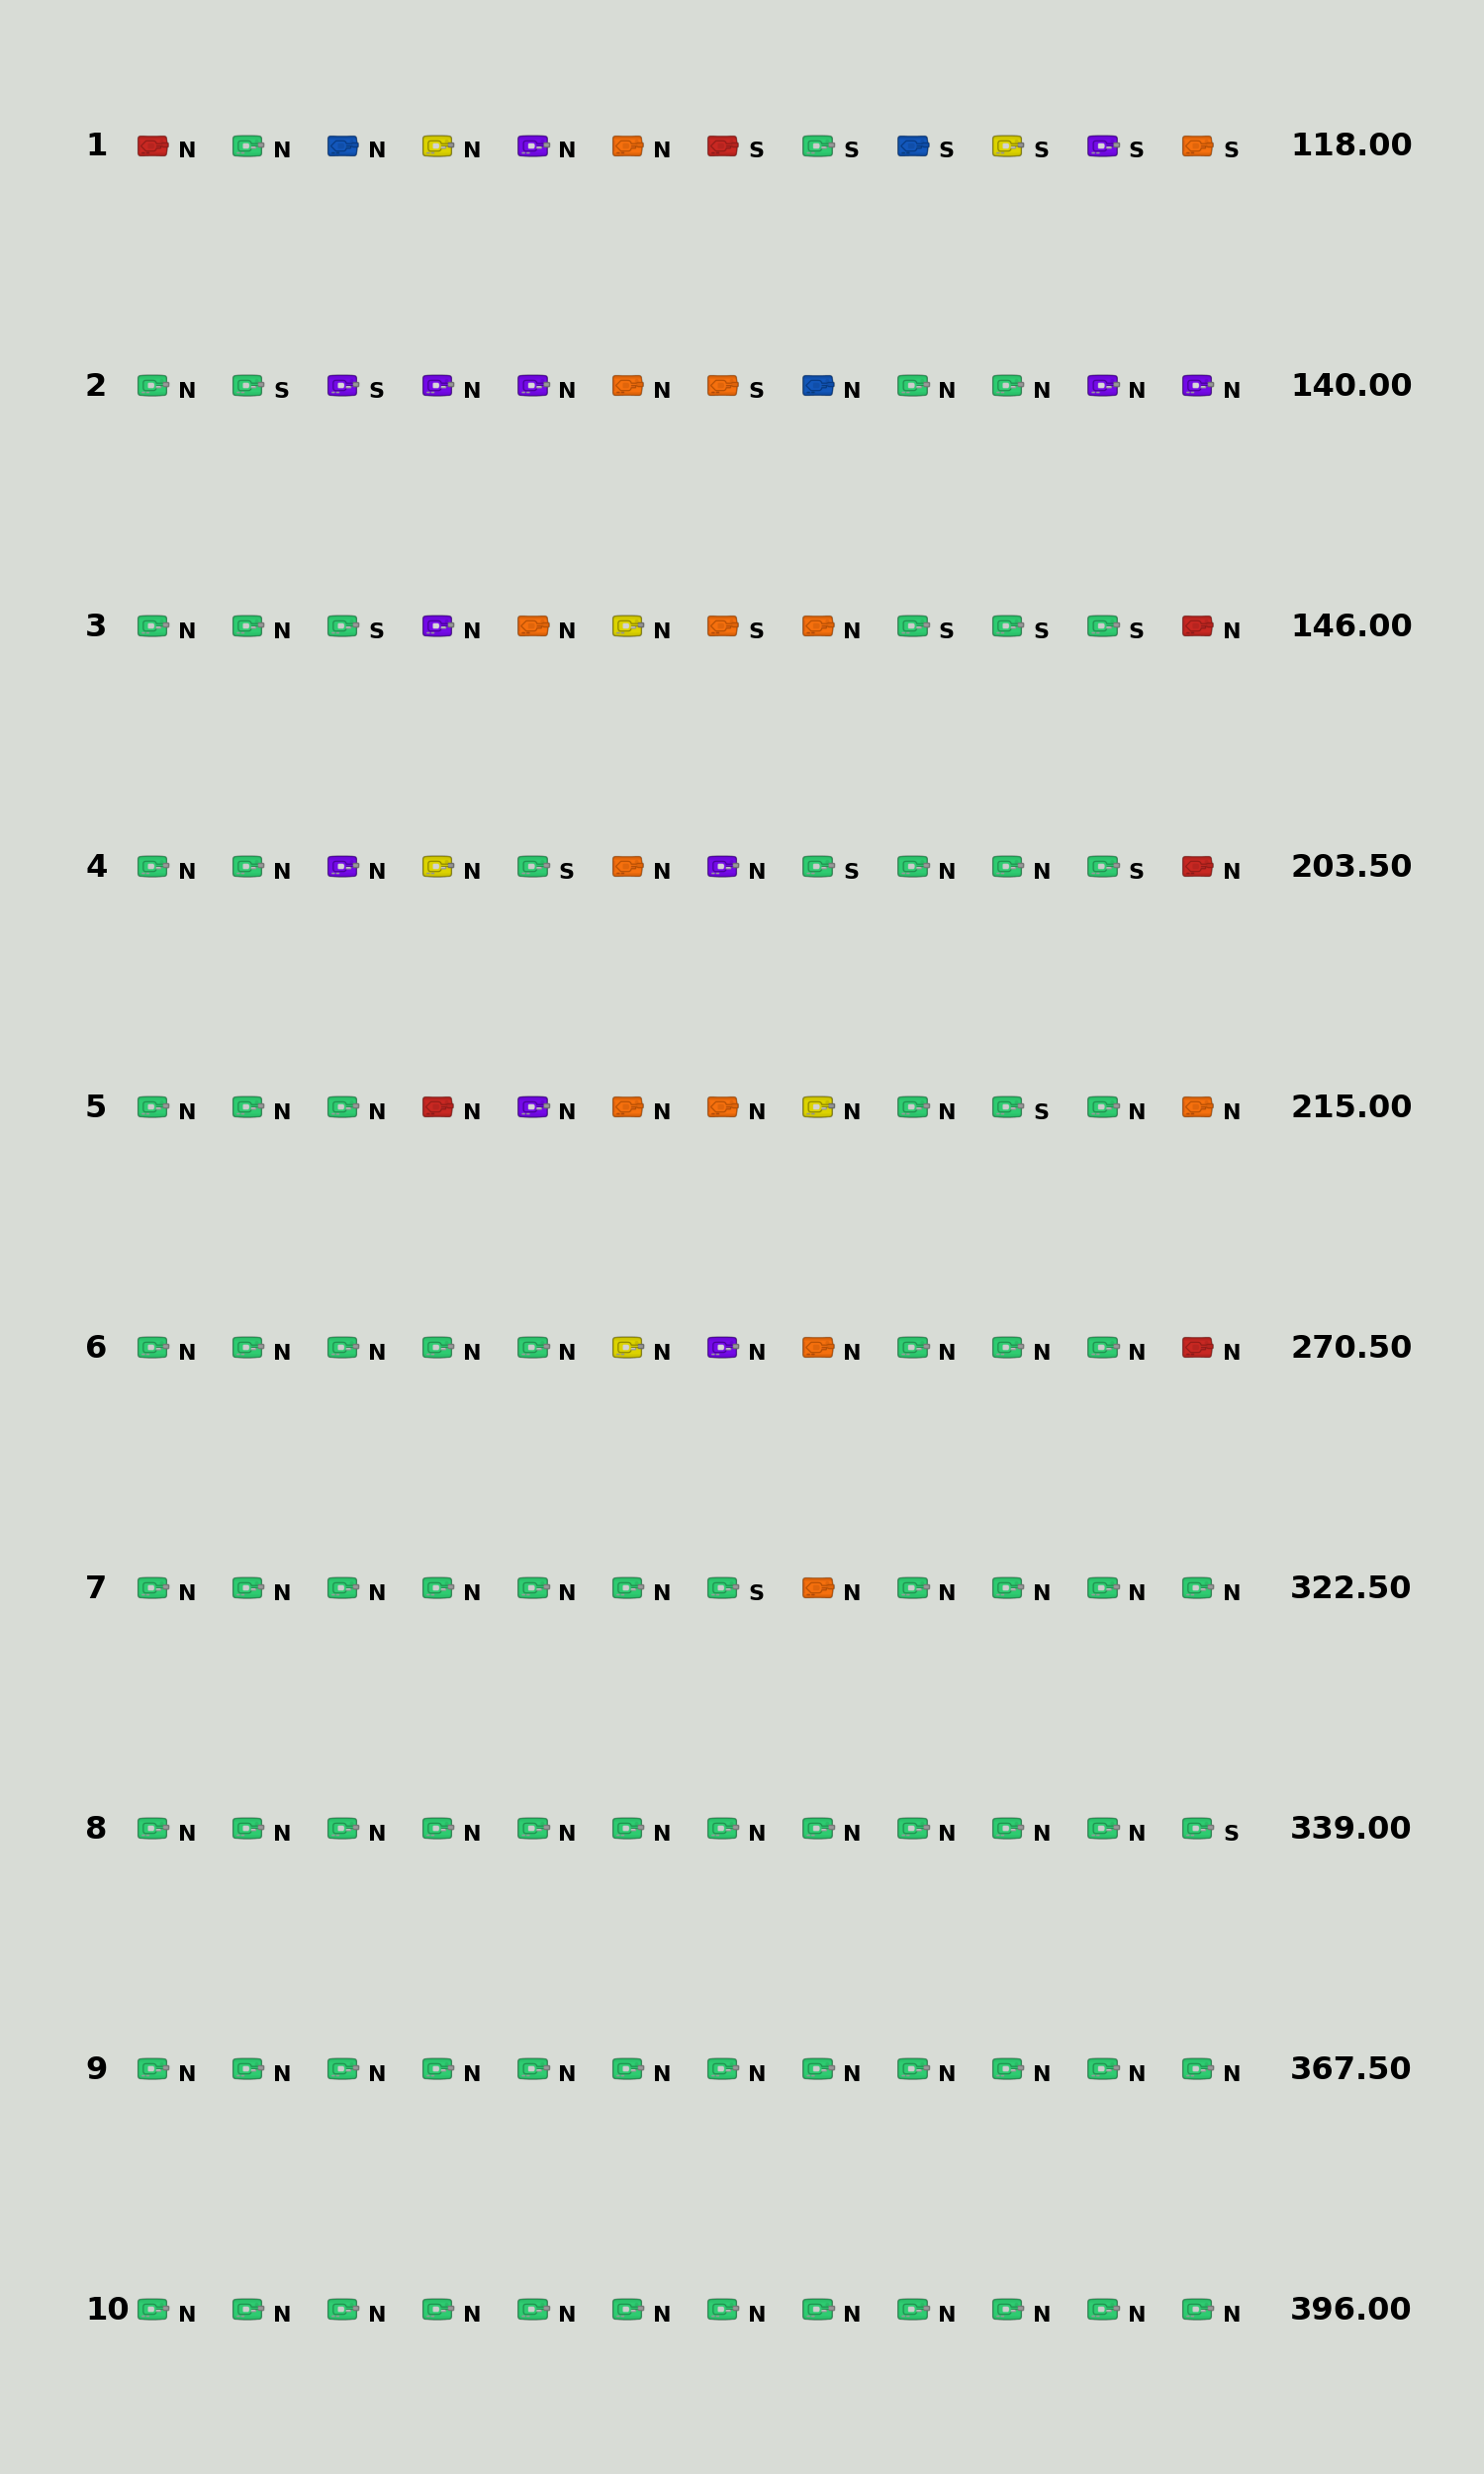
\includegraphics[width=0.9\textwidth]{figuras/td/td_allgreen_ai_mode_2_1.png}
  \caption{Visualização da moda de cada onda com a versão v2 contra Torres Verdes.}
  \label{fig:td-moda-green-2-1}
\end{figure}

\begin{figure}[H]
  \centering
  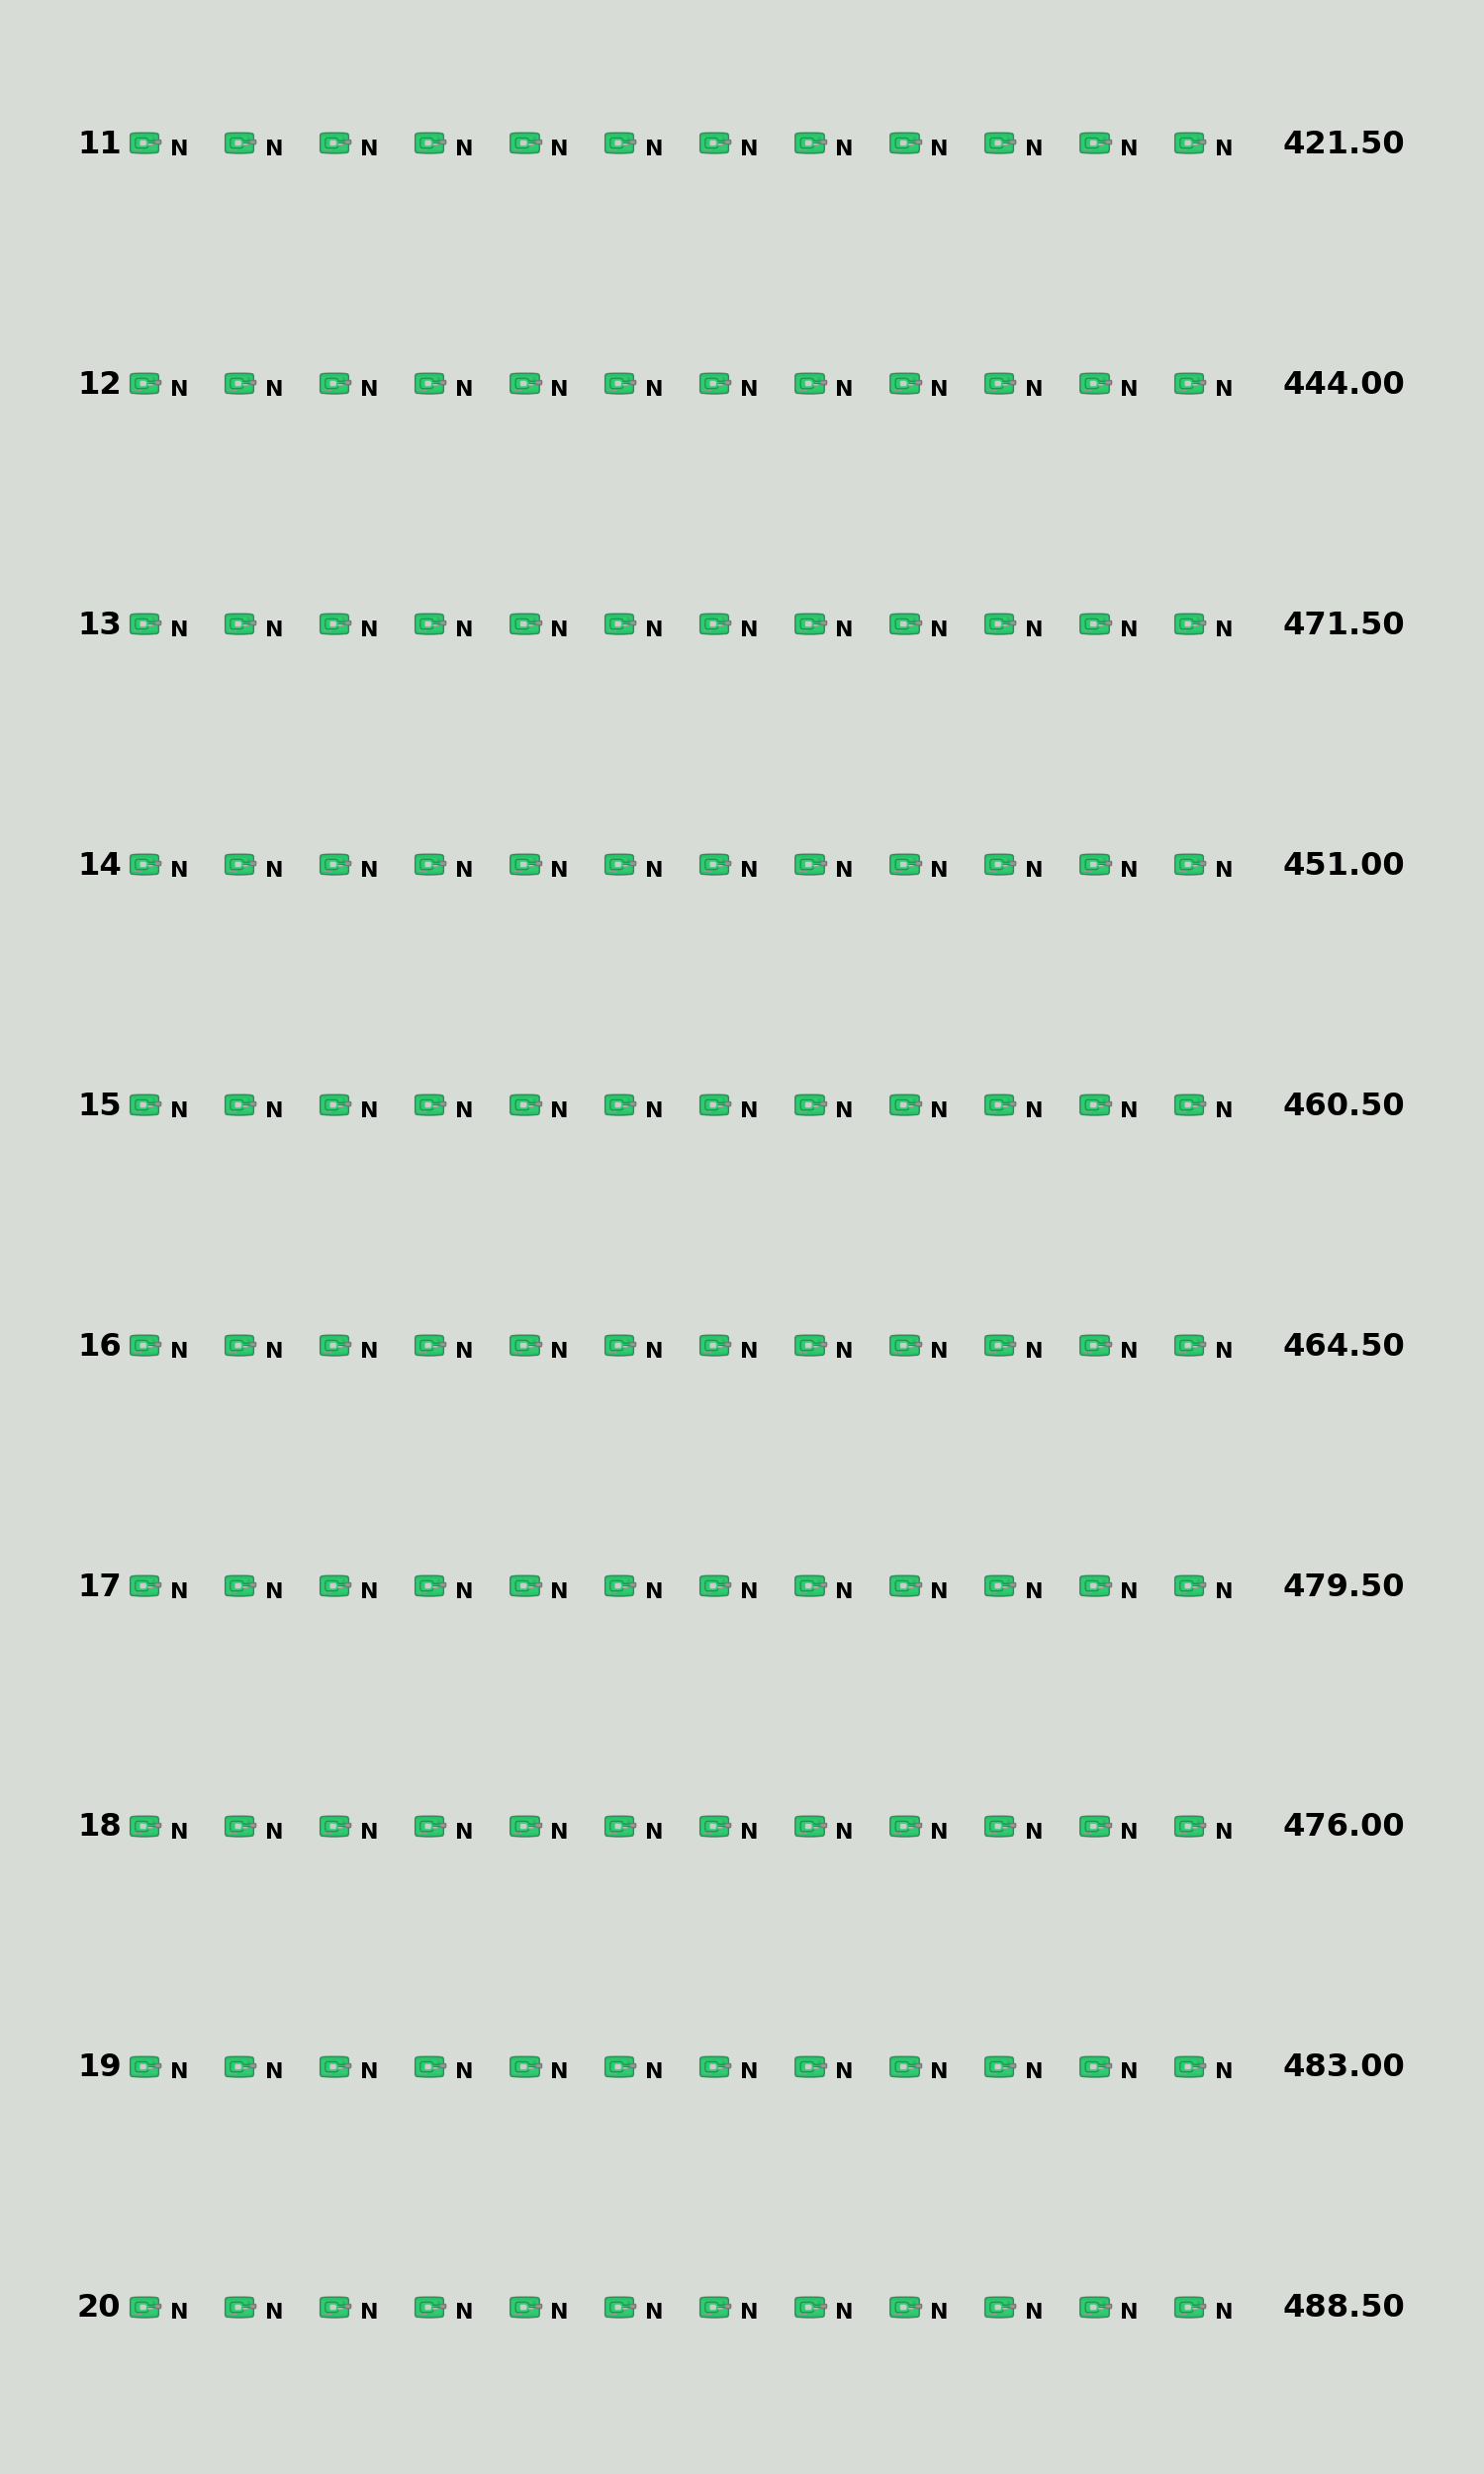
\includegraphics[width=0.9\textwidth]{figuras/td/td_allgreen_ai_mode_2_2.png}
  \caption{Visualização da moda de cada onda com a versão v2 contra Torres Verdes.}
  \label{fig:td-moda-green-2-2}
\end{figure}

\begin{figure}[H]
  \centering
  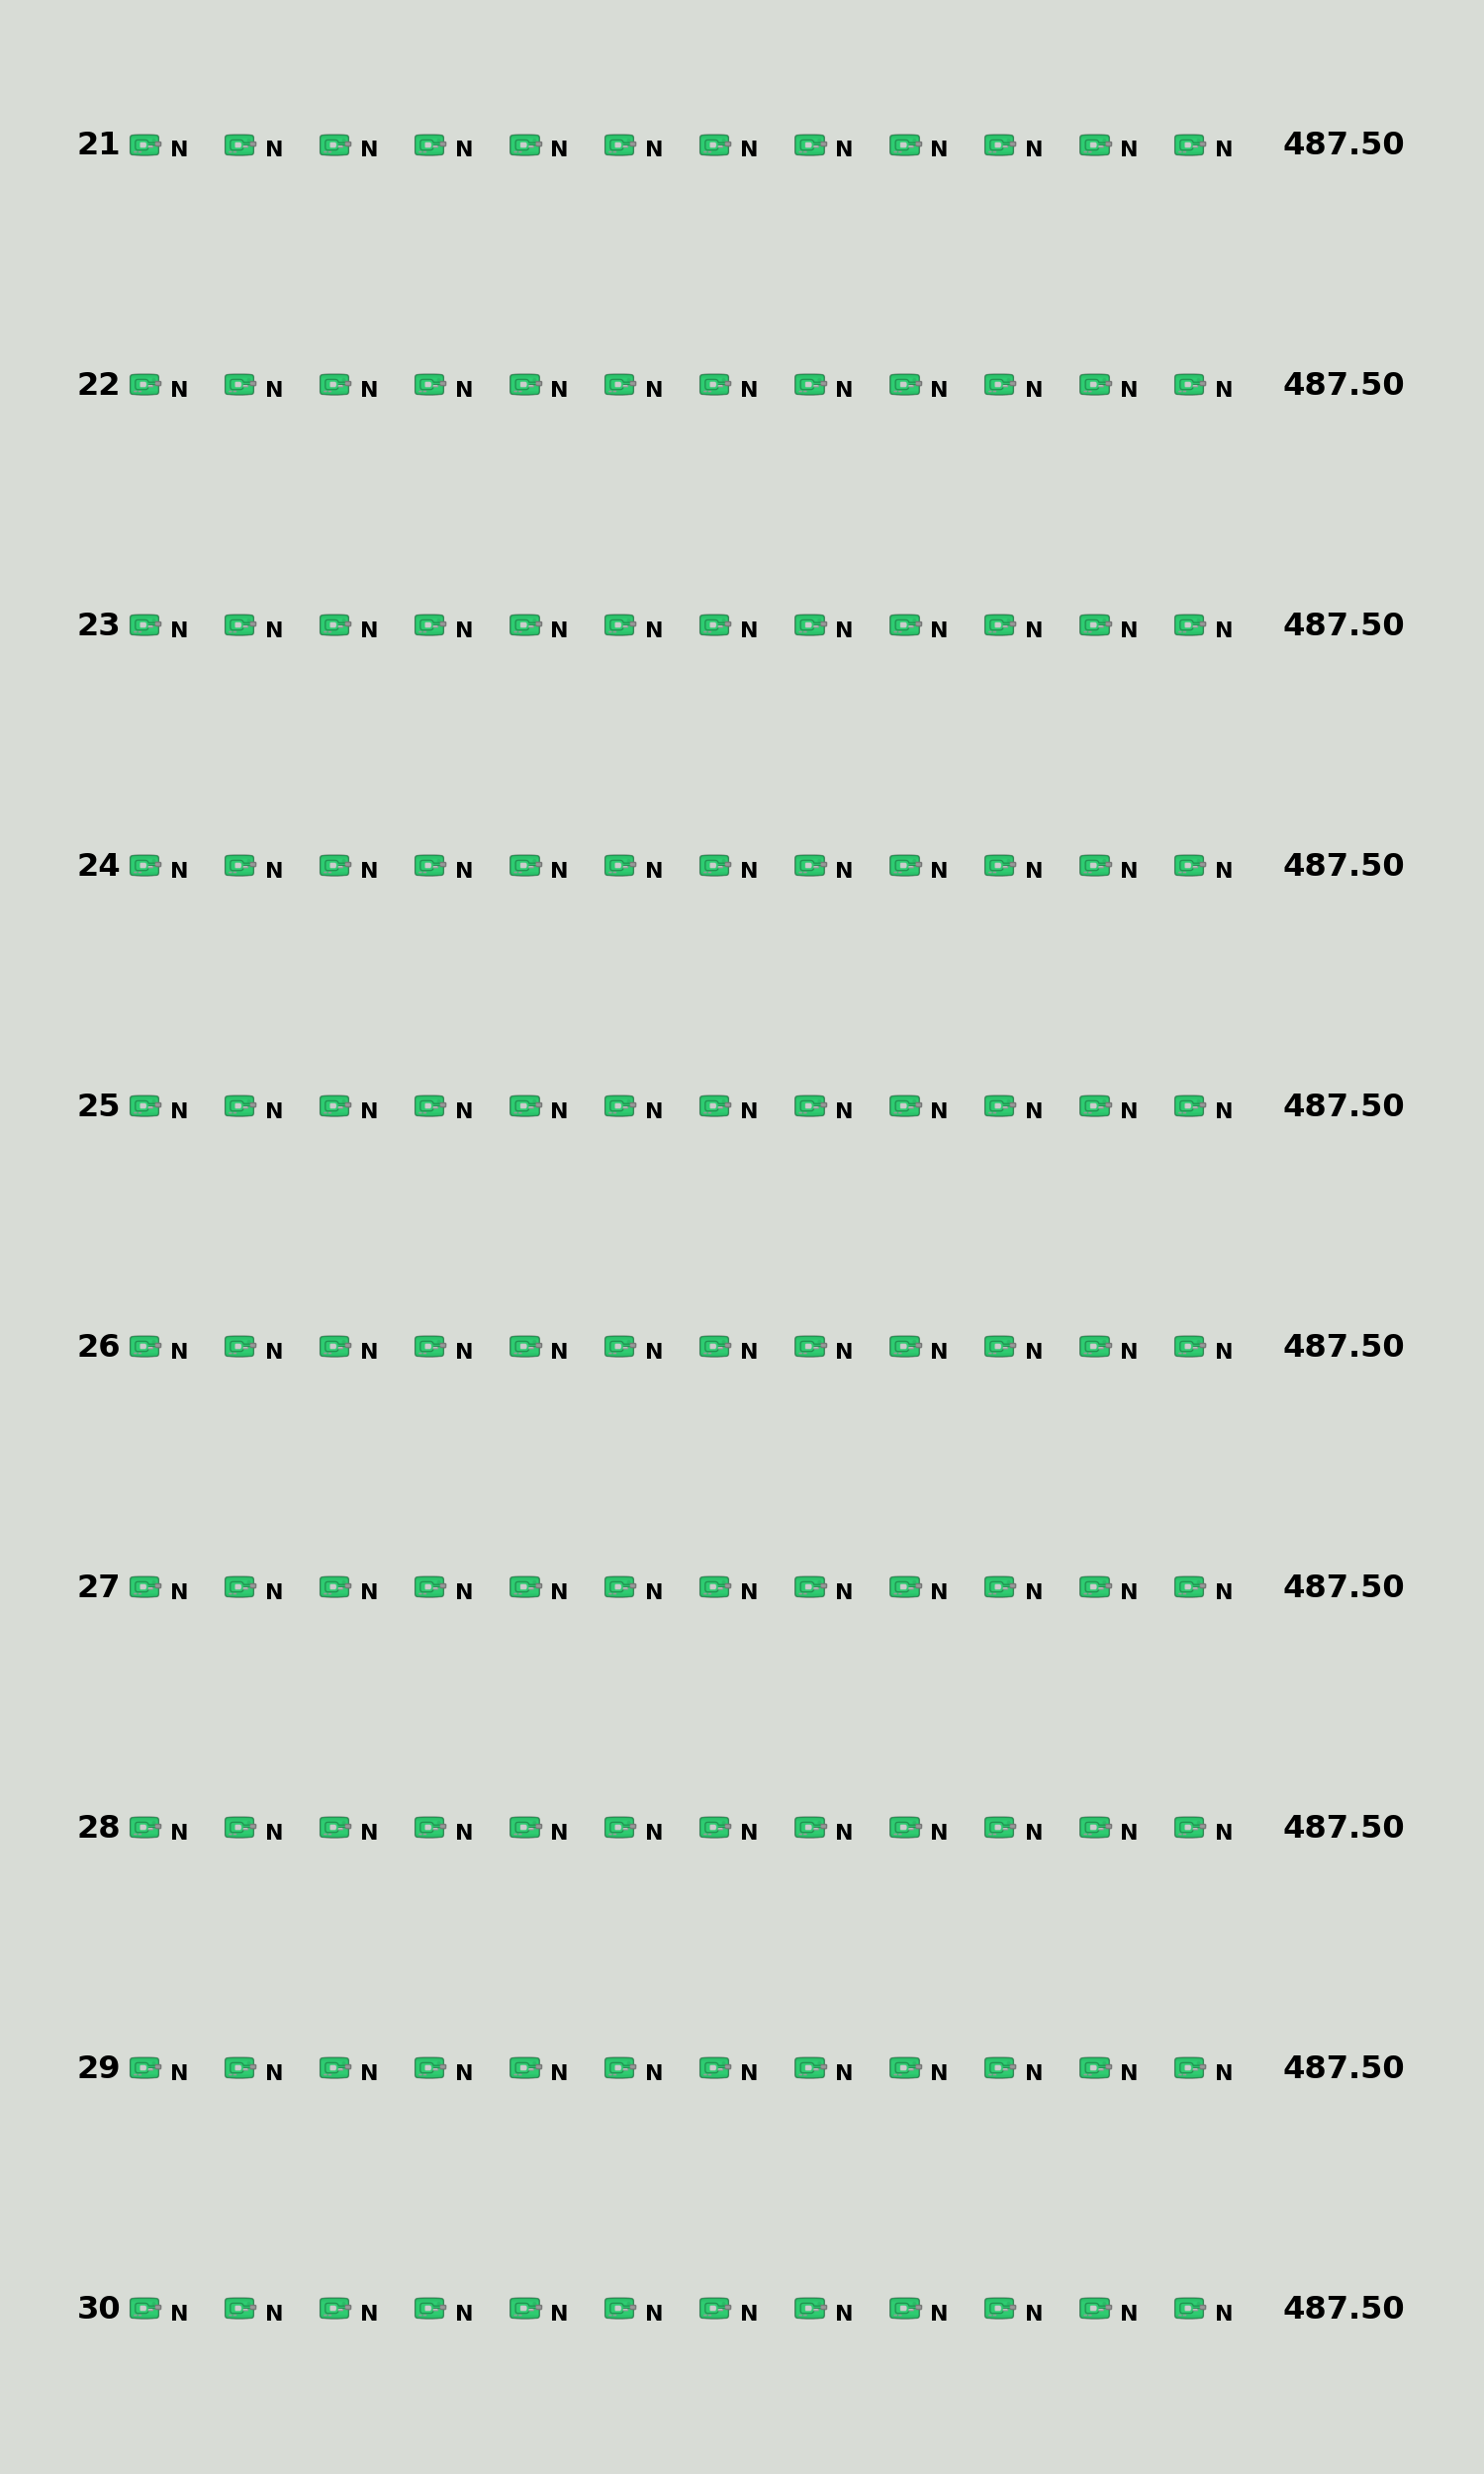
\includegraphics[width=0.9\textwidth]{figuras/td/td_allgreen_ai_mode_2_3.png}
  \caption{Visualização da moda de cada onda com a versão v2 contra Torres Verdes.}
  \label{fig:td-moda-green-2-3}
\end{figure}

%% ------------------------------------------------------------------------- %%
\section{Torres Vermelhas}
\label{sec:apend-moda-td-r-v2}

\begin{figure}[H]
  \centering
  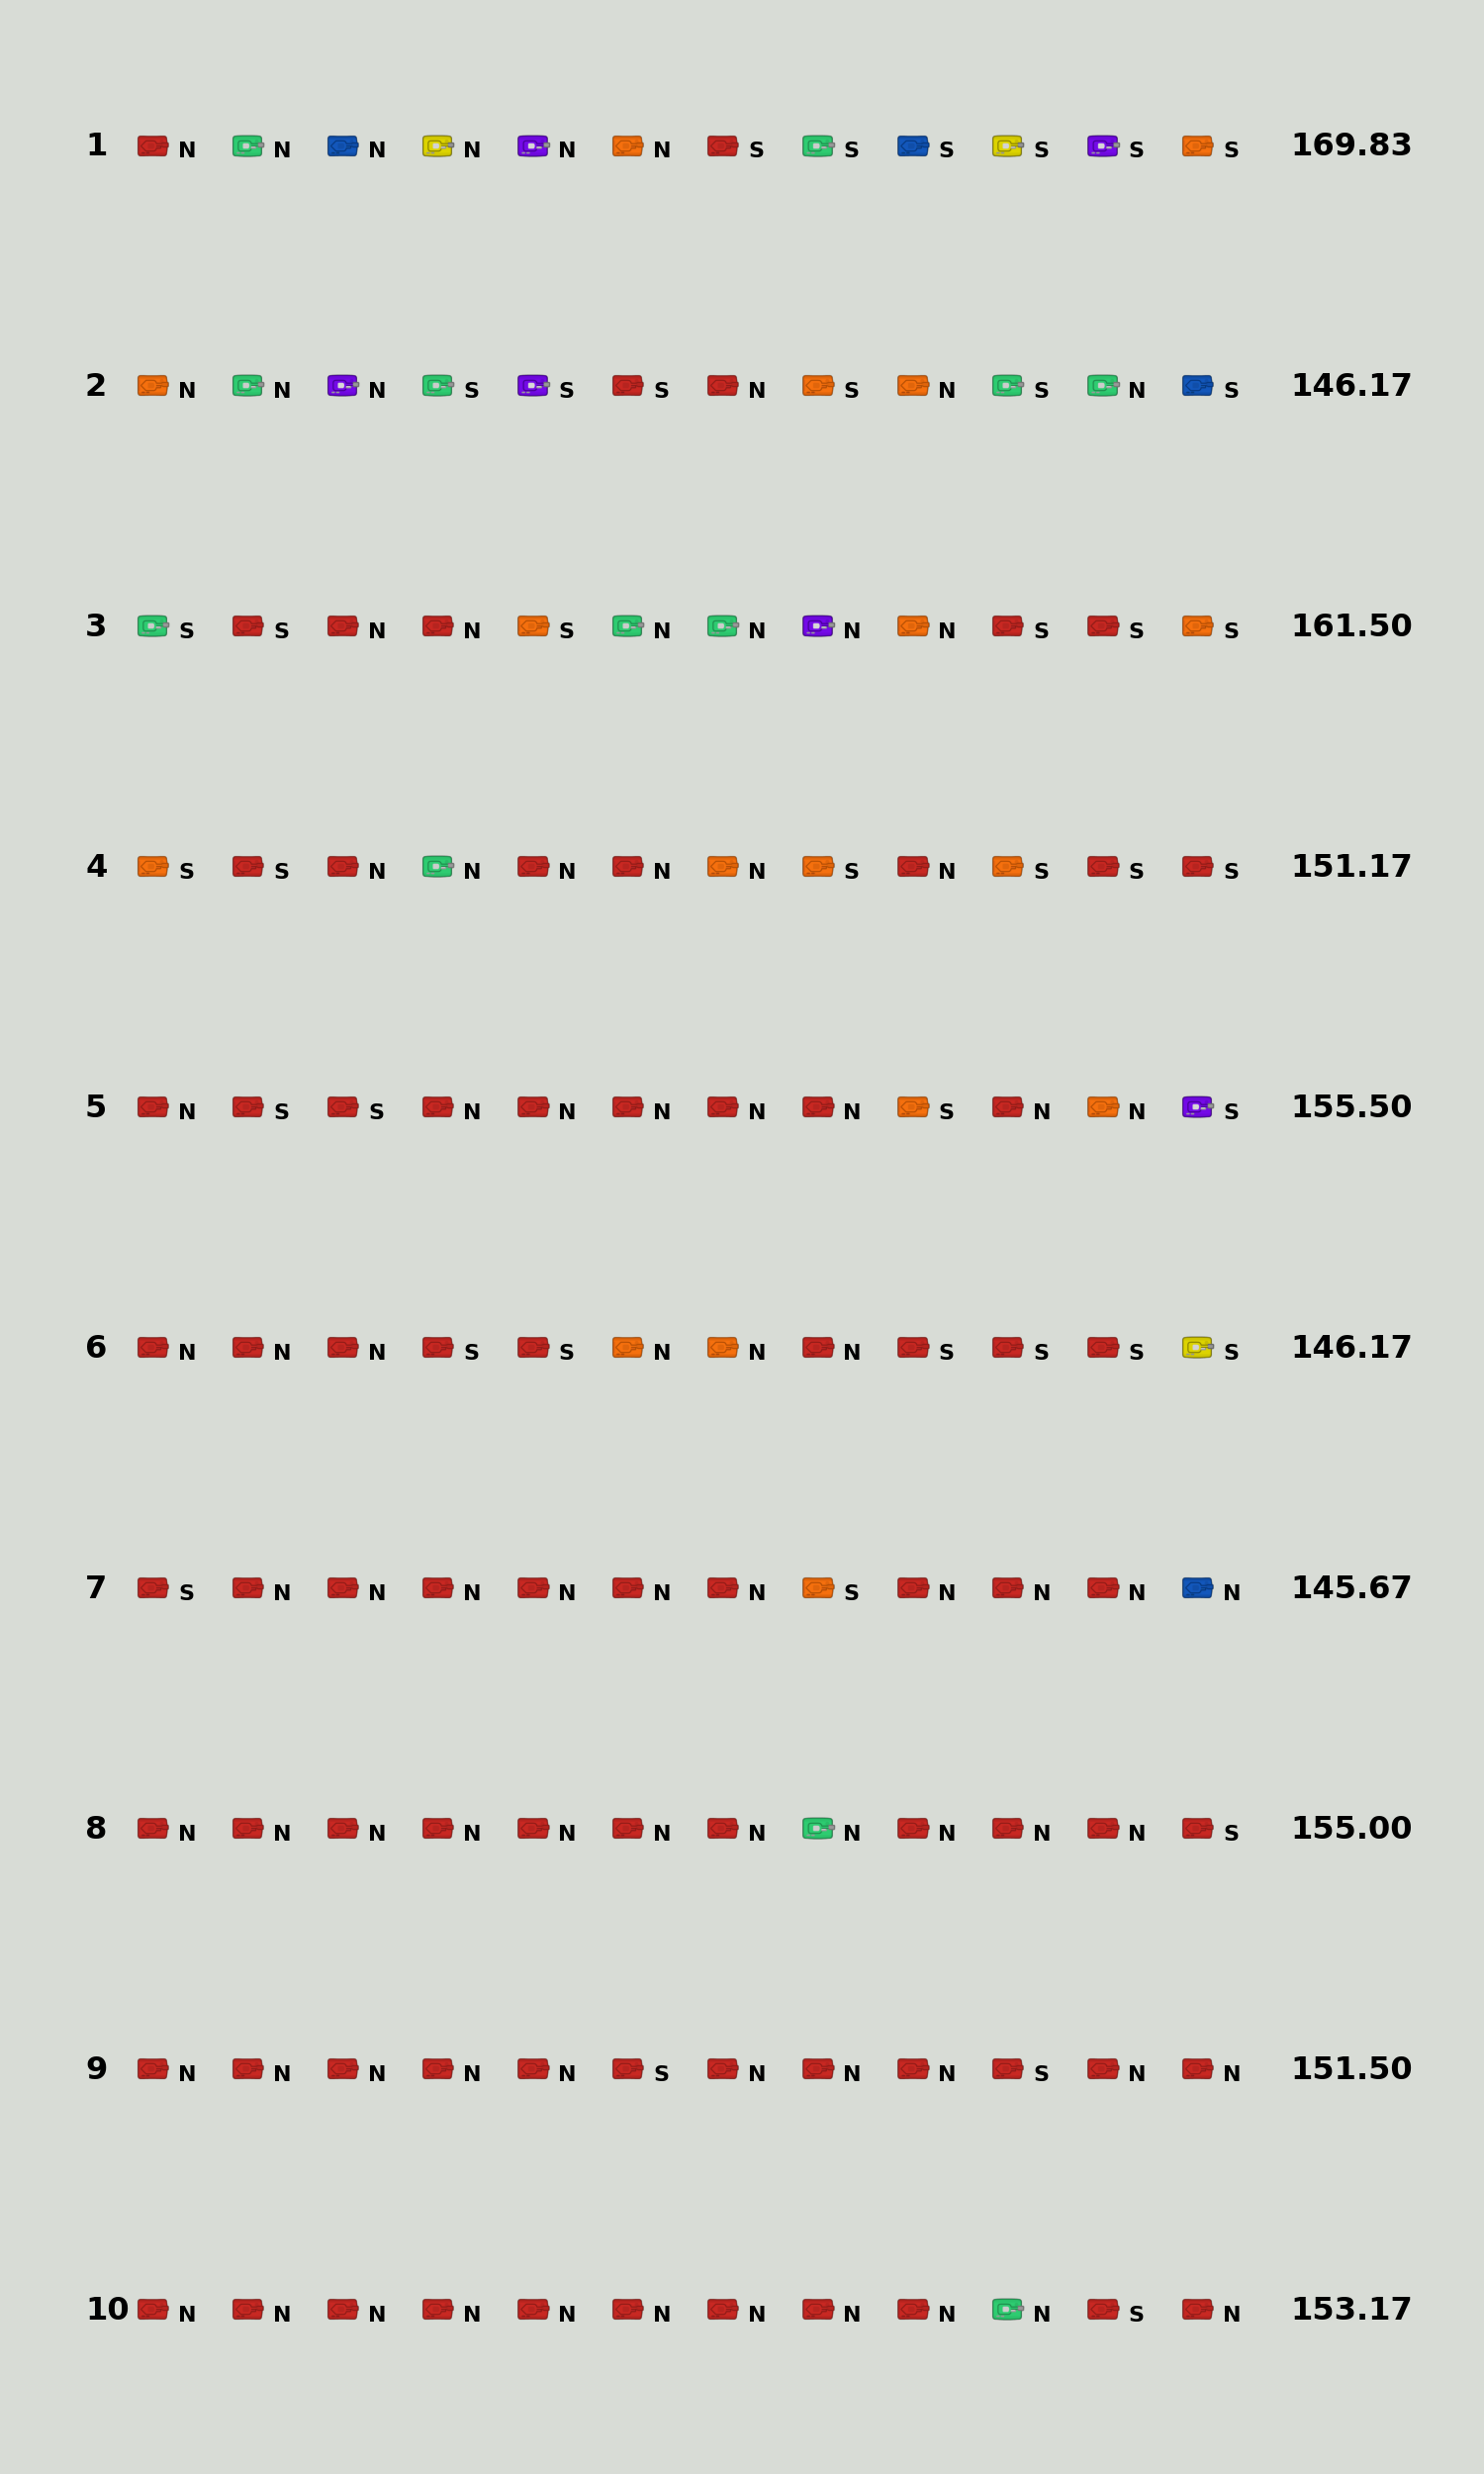
\includegraphics[width=0.9\textwidth]{figuras/td/td_allred_ai_mode_2_1.png}
  \caption{Visualização da moda de cada onda com a versão v2 contra Torres Vermelhas.}
  \label{fig:td-moda-red-2-1}
\end{figure}

\begin{figure}[H]
  \centering
  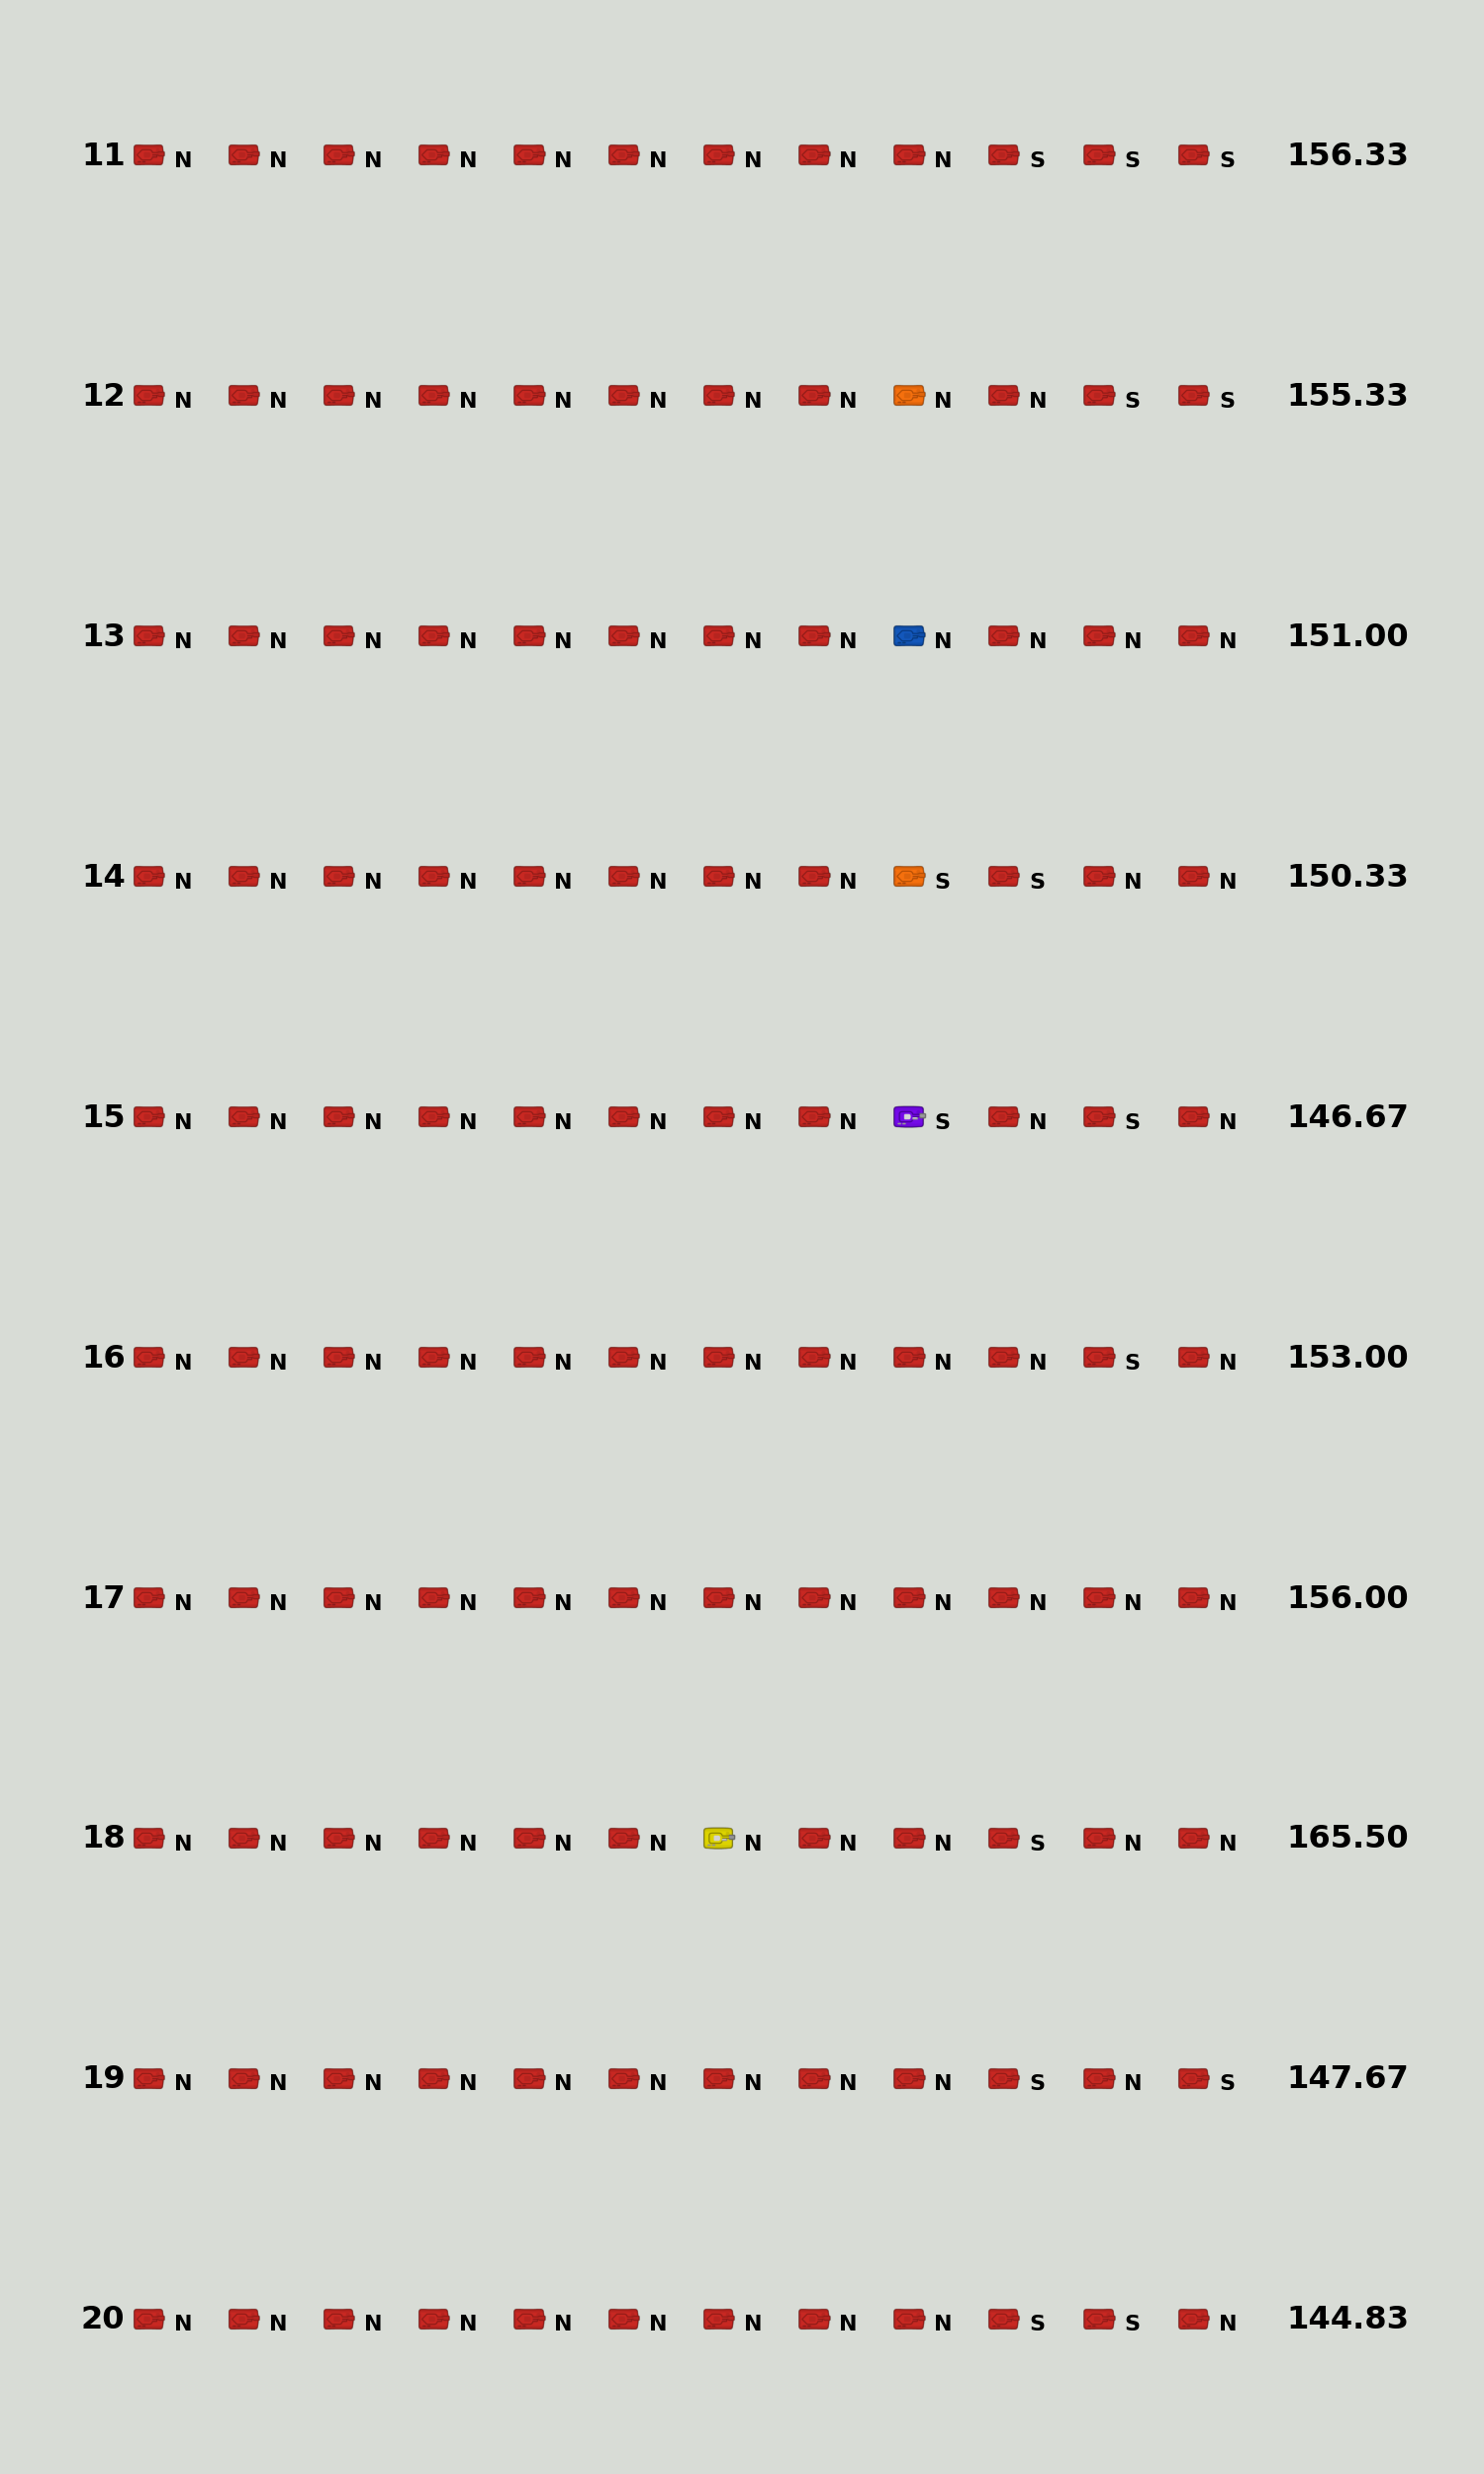
\includegraphics[width=0.9\textwidth]{figuras/td/td_allred_ai_mode_2_2.png}
  \caption{Visualização da moda de cada onda com a versão v2 contra Torres Vermelhas.}
  \label{fig:td-moda-red-2-2}
\end{figure}

\begin{figure}[H]
  \centering
  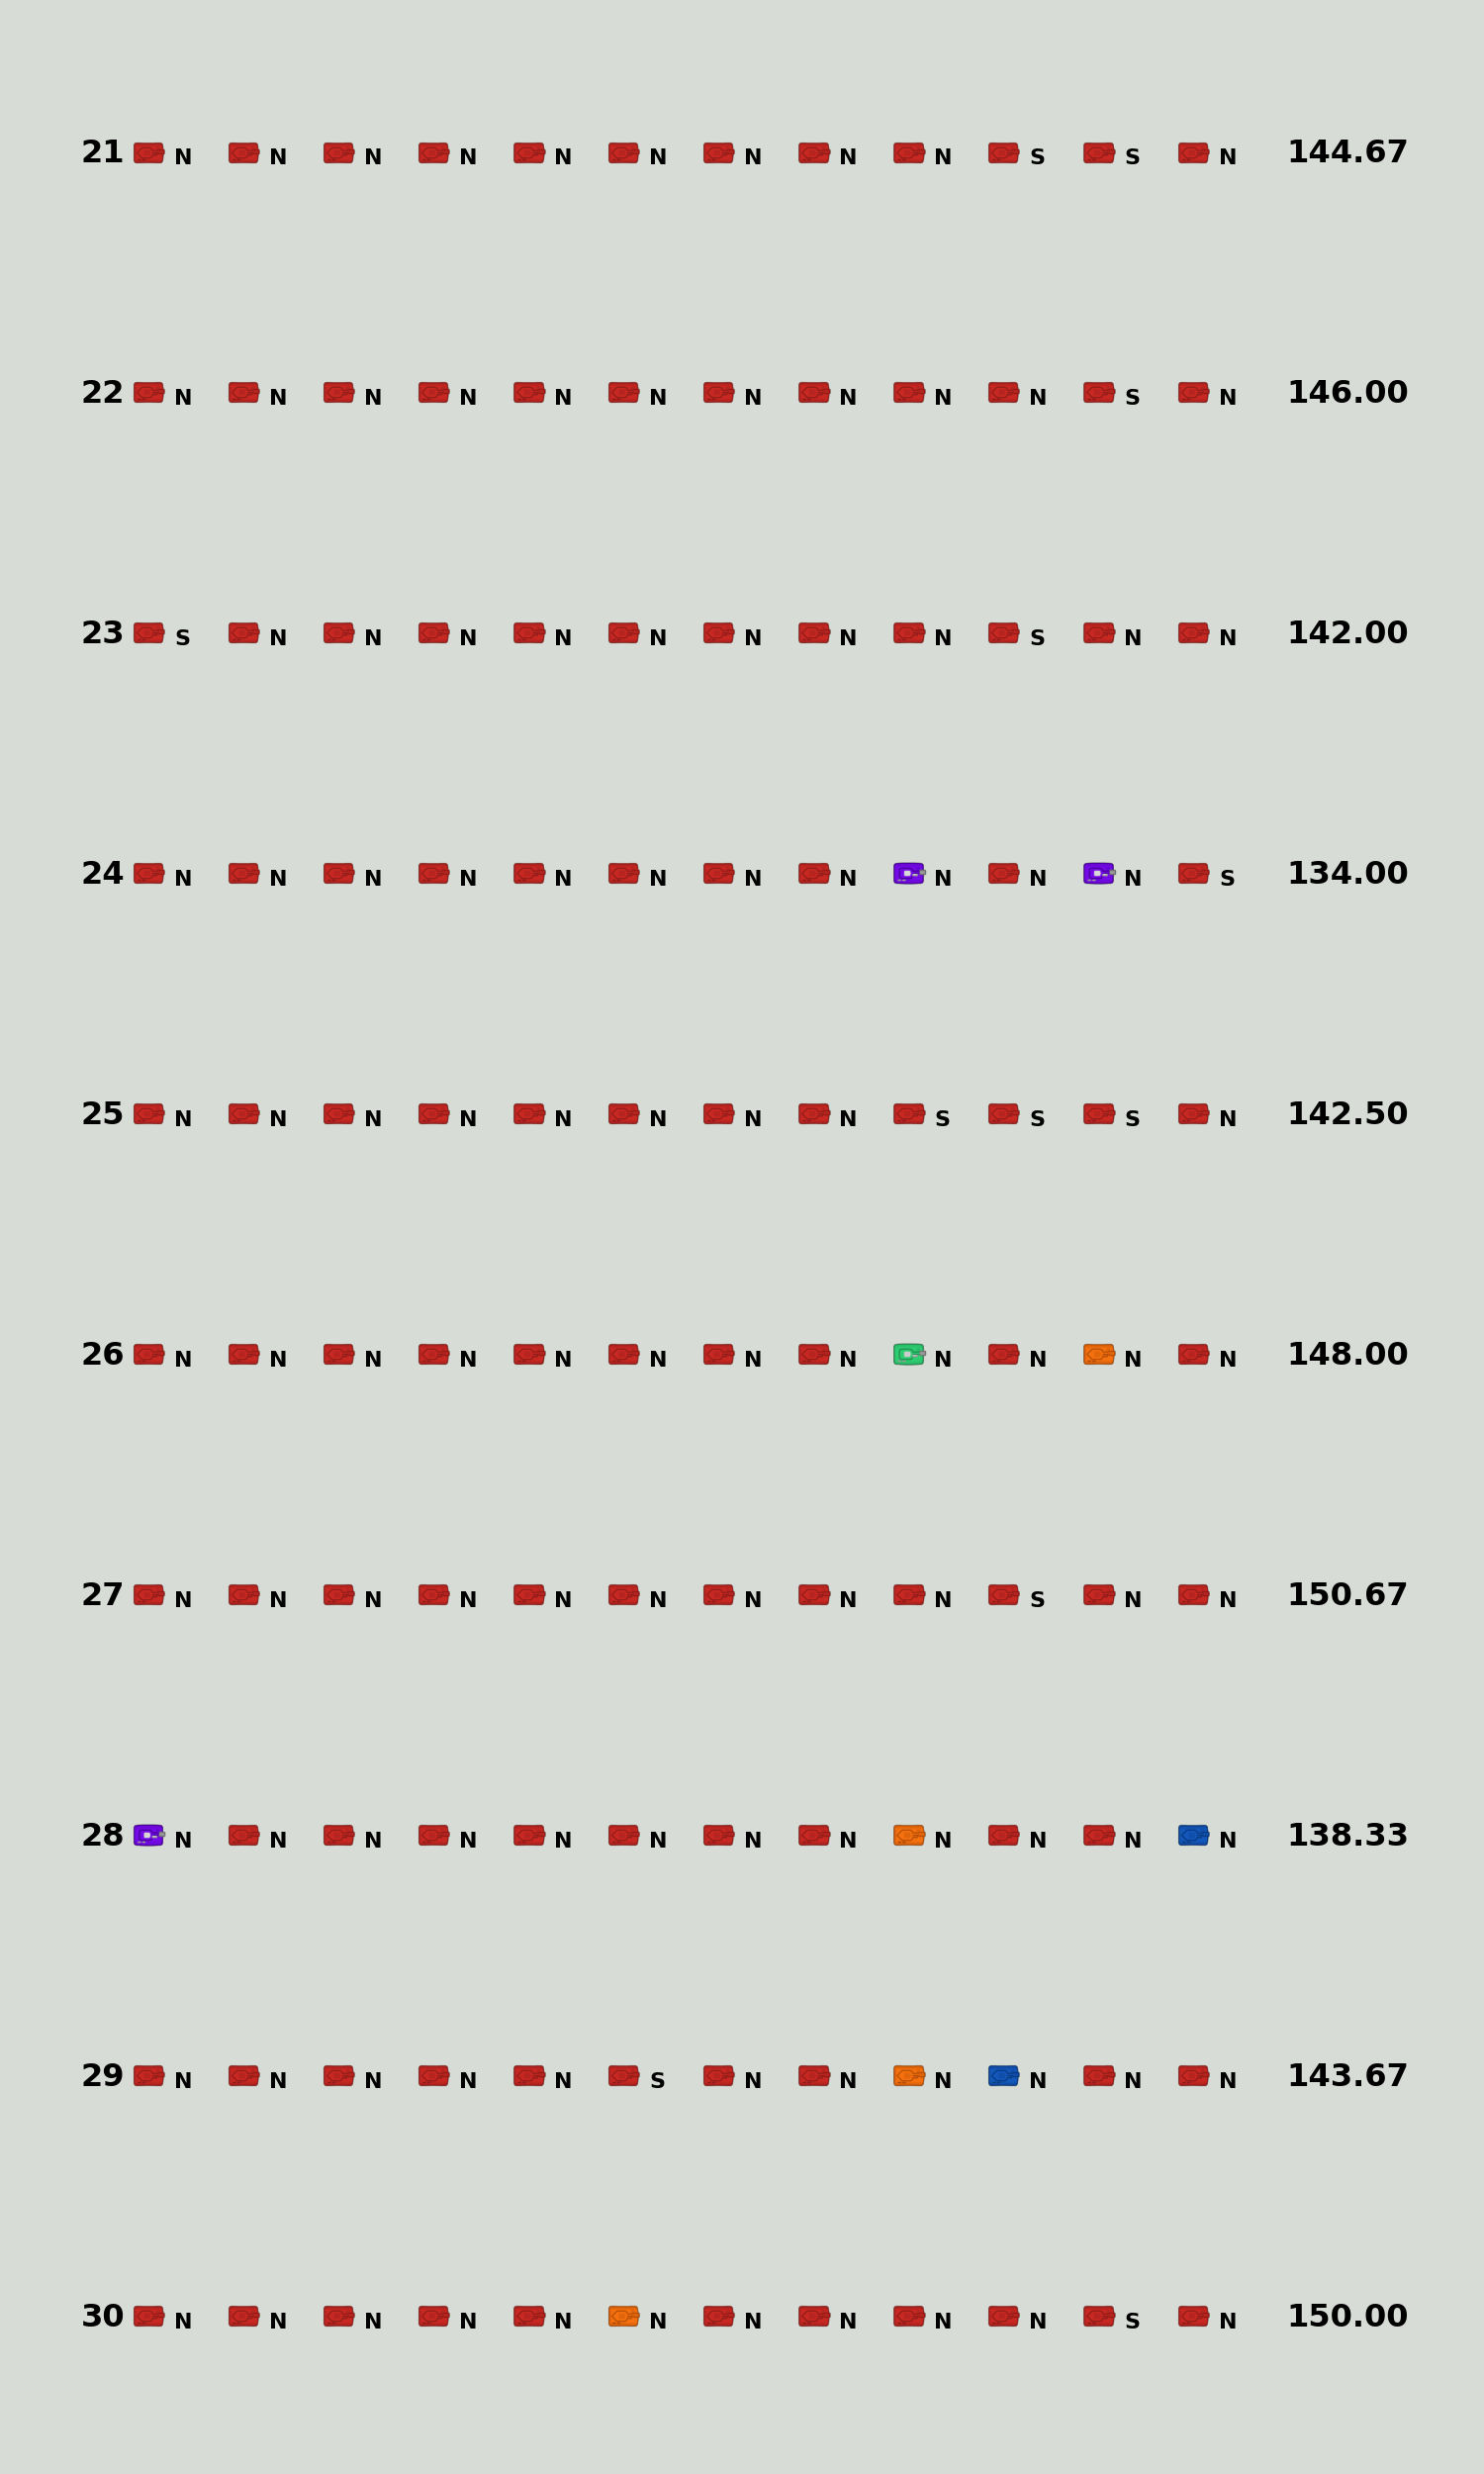
\includegraphics[width=0.9\textwidth]{figuras/td/td_allred_ai_mode_2_3.png}
  \caption{Visualização da moda de cada onda com a versão v2 contra Torres Vermelhas.}
  \label{fig:td-moda-red-2-3}
\end{figure}

%% ------------------------------------------------------------------------- %%
\section{Torres Verde + Vermelha}
\label{sec:apend-moda-td-gr-v2}

\begin{figure}[H]
  \centering
  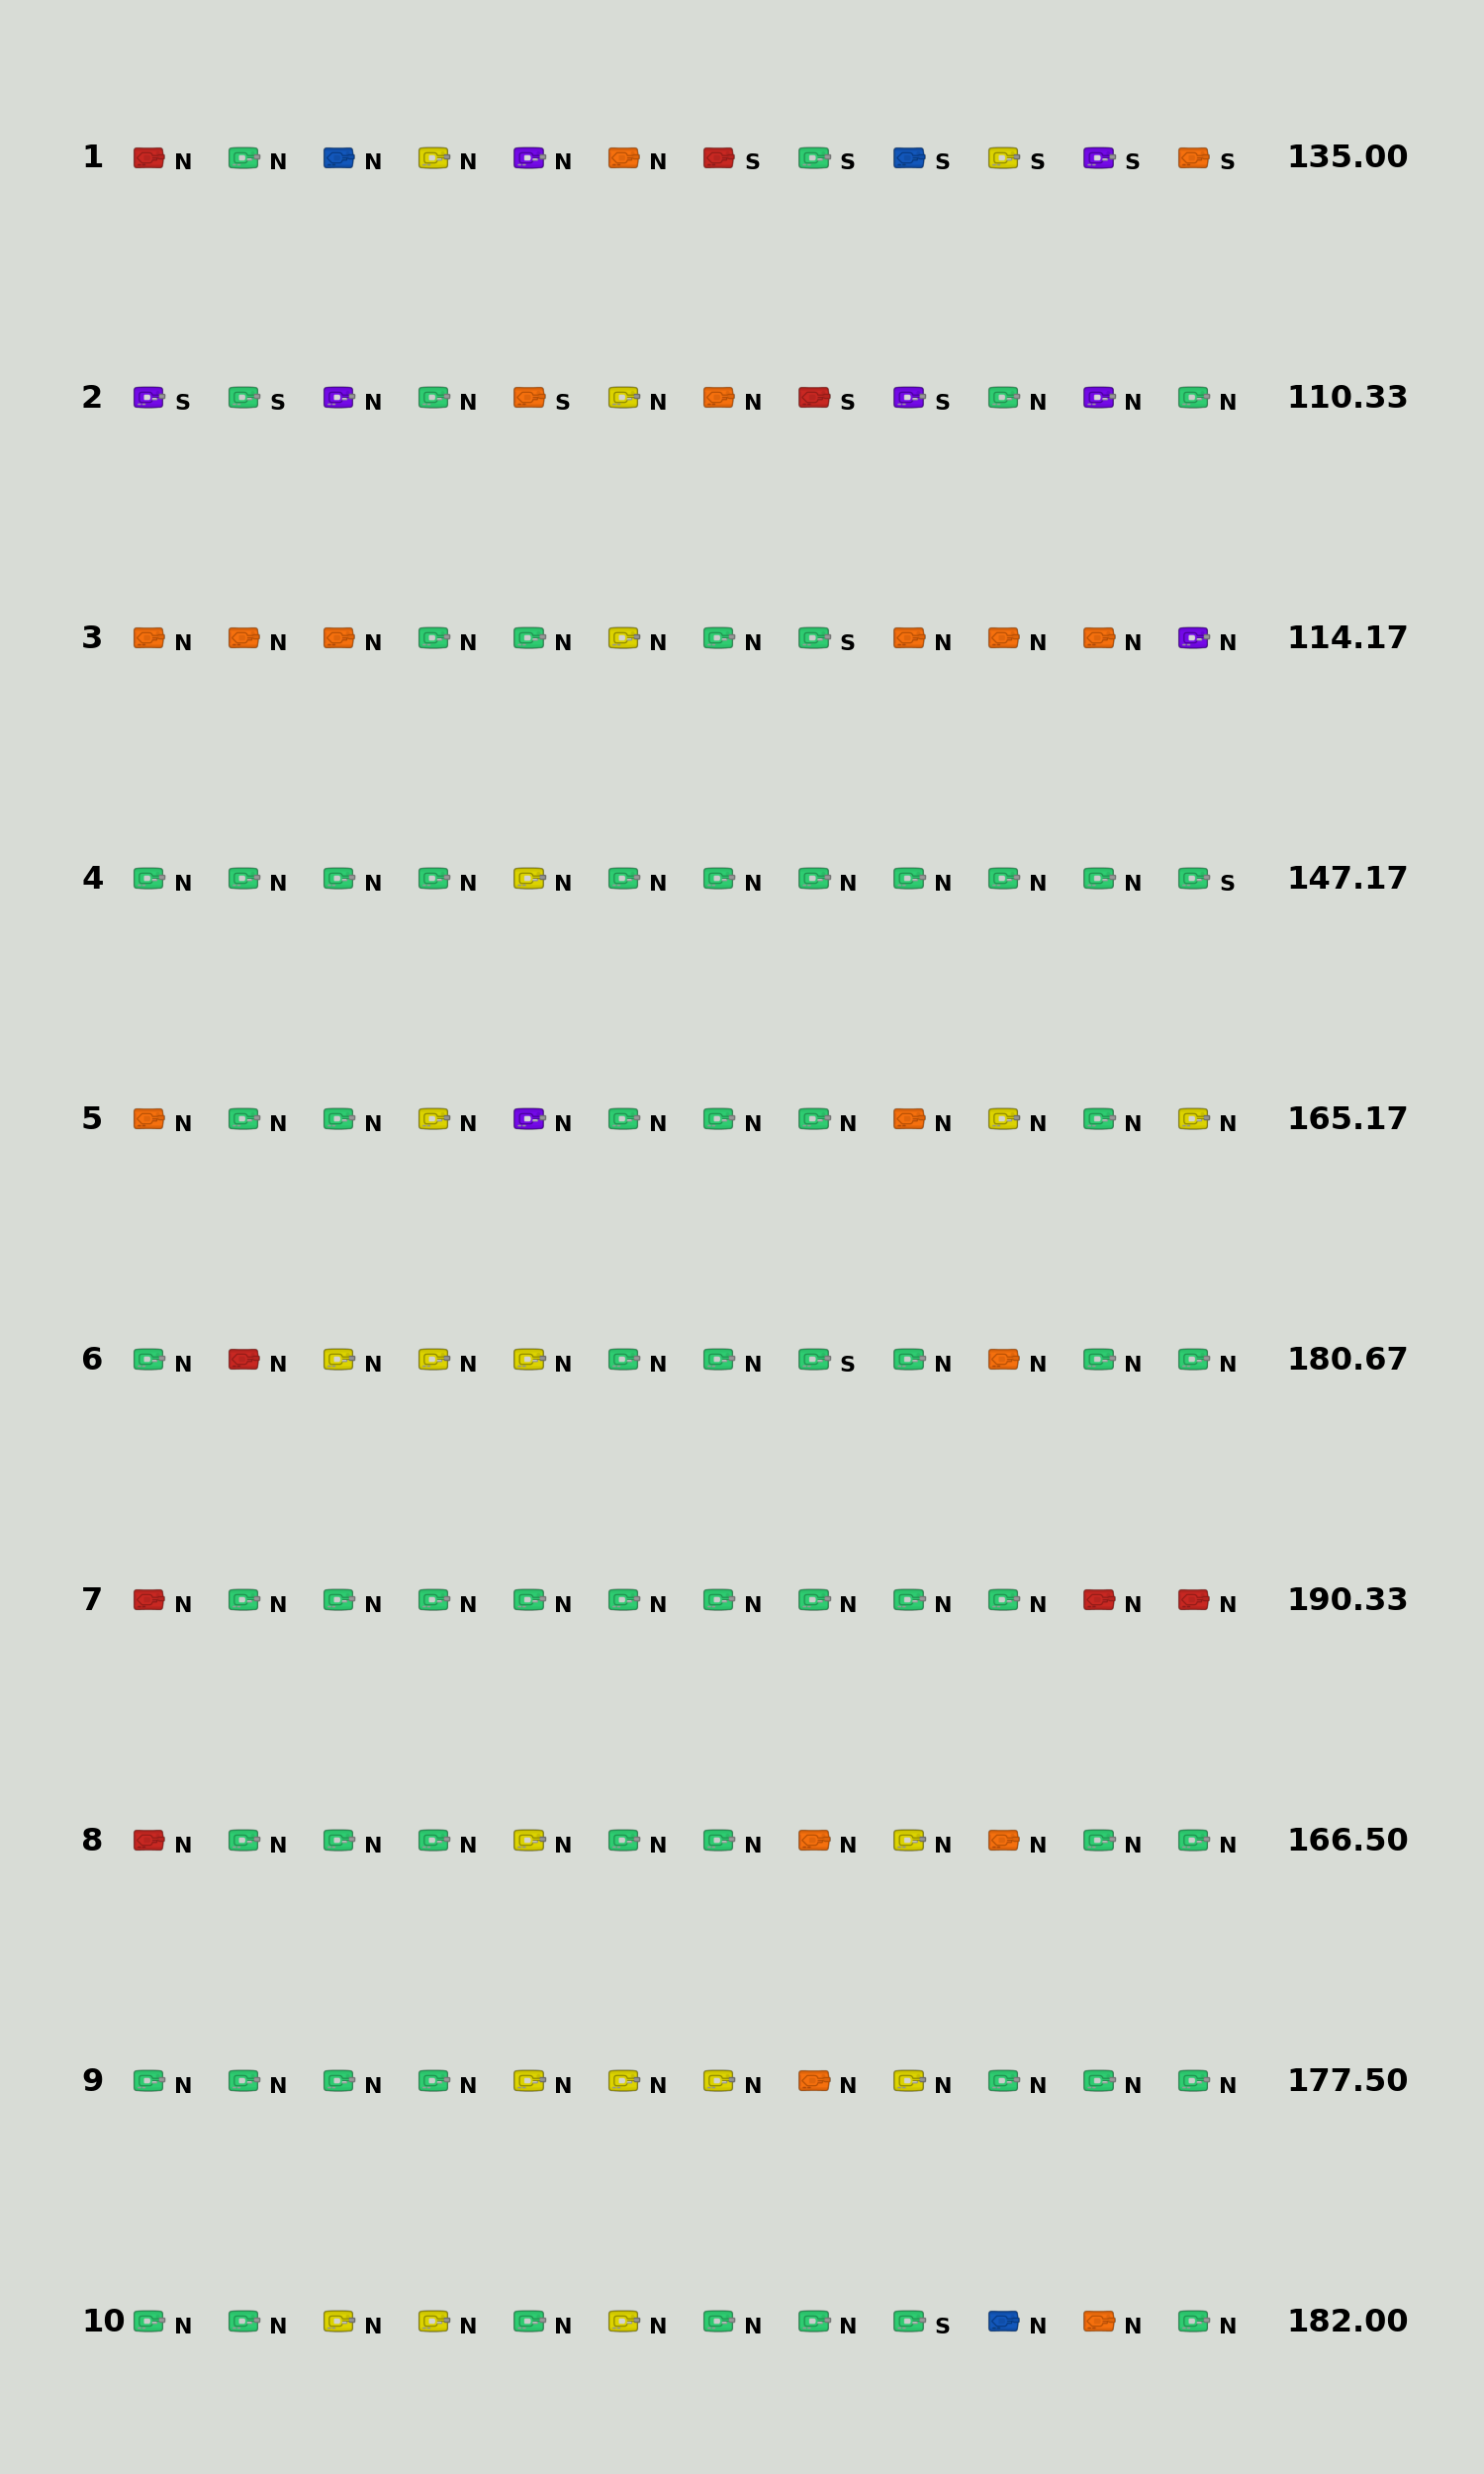
\includegraphics[width=0.9\textwidth]{figuras/td/td_greenred_ai_mode_2_1.png}
  \caption{Visualização da moda de cada onda com a versão v2 contra Torres Verdes + Vermelhas.}
  \label{fig:td-moda-greenred-2-1}
\end{figure}

\begin{figure}[H]
  \centering
  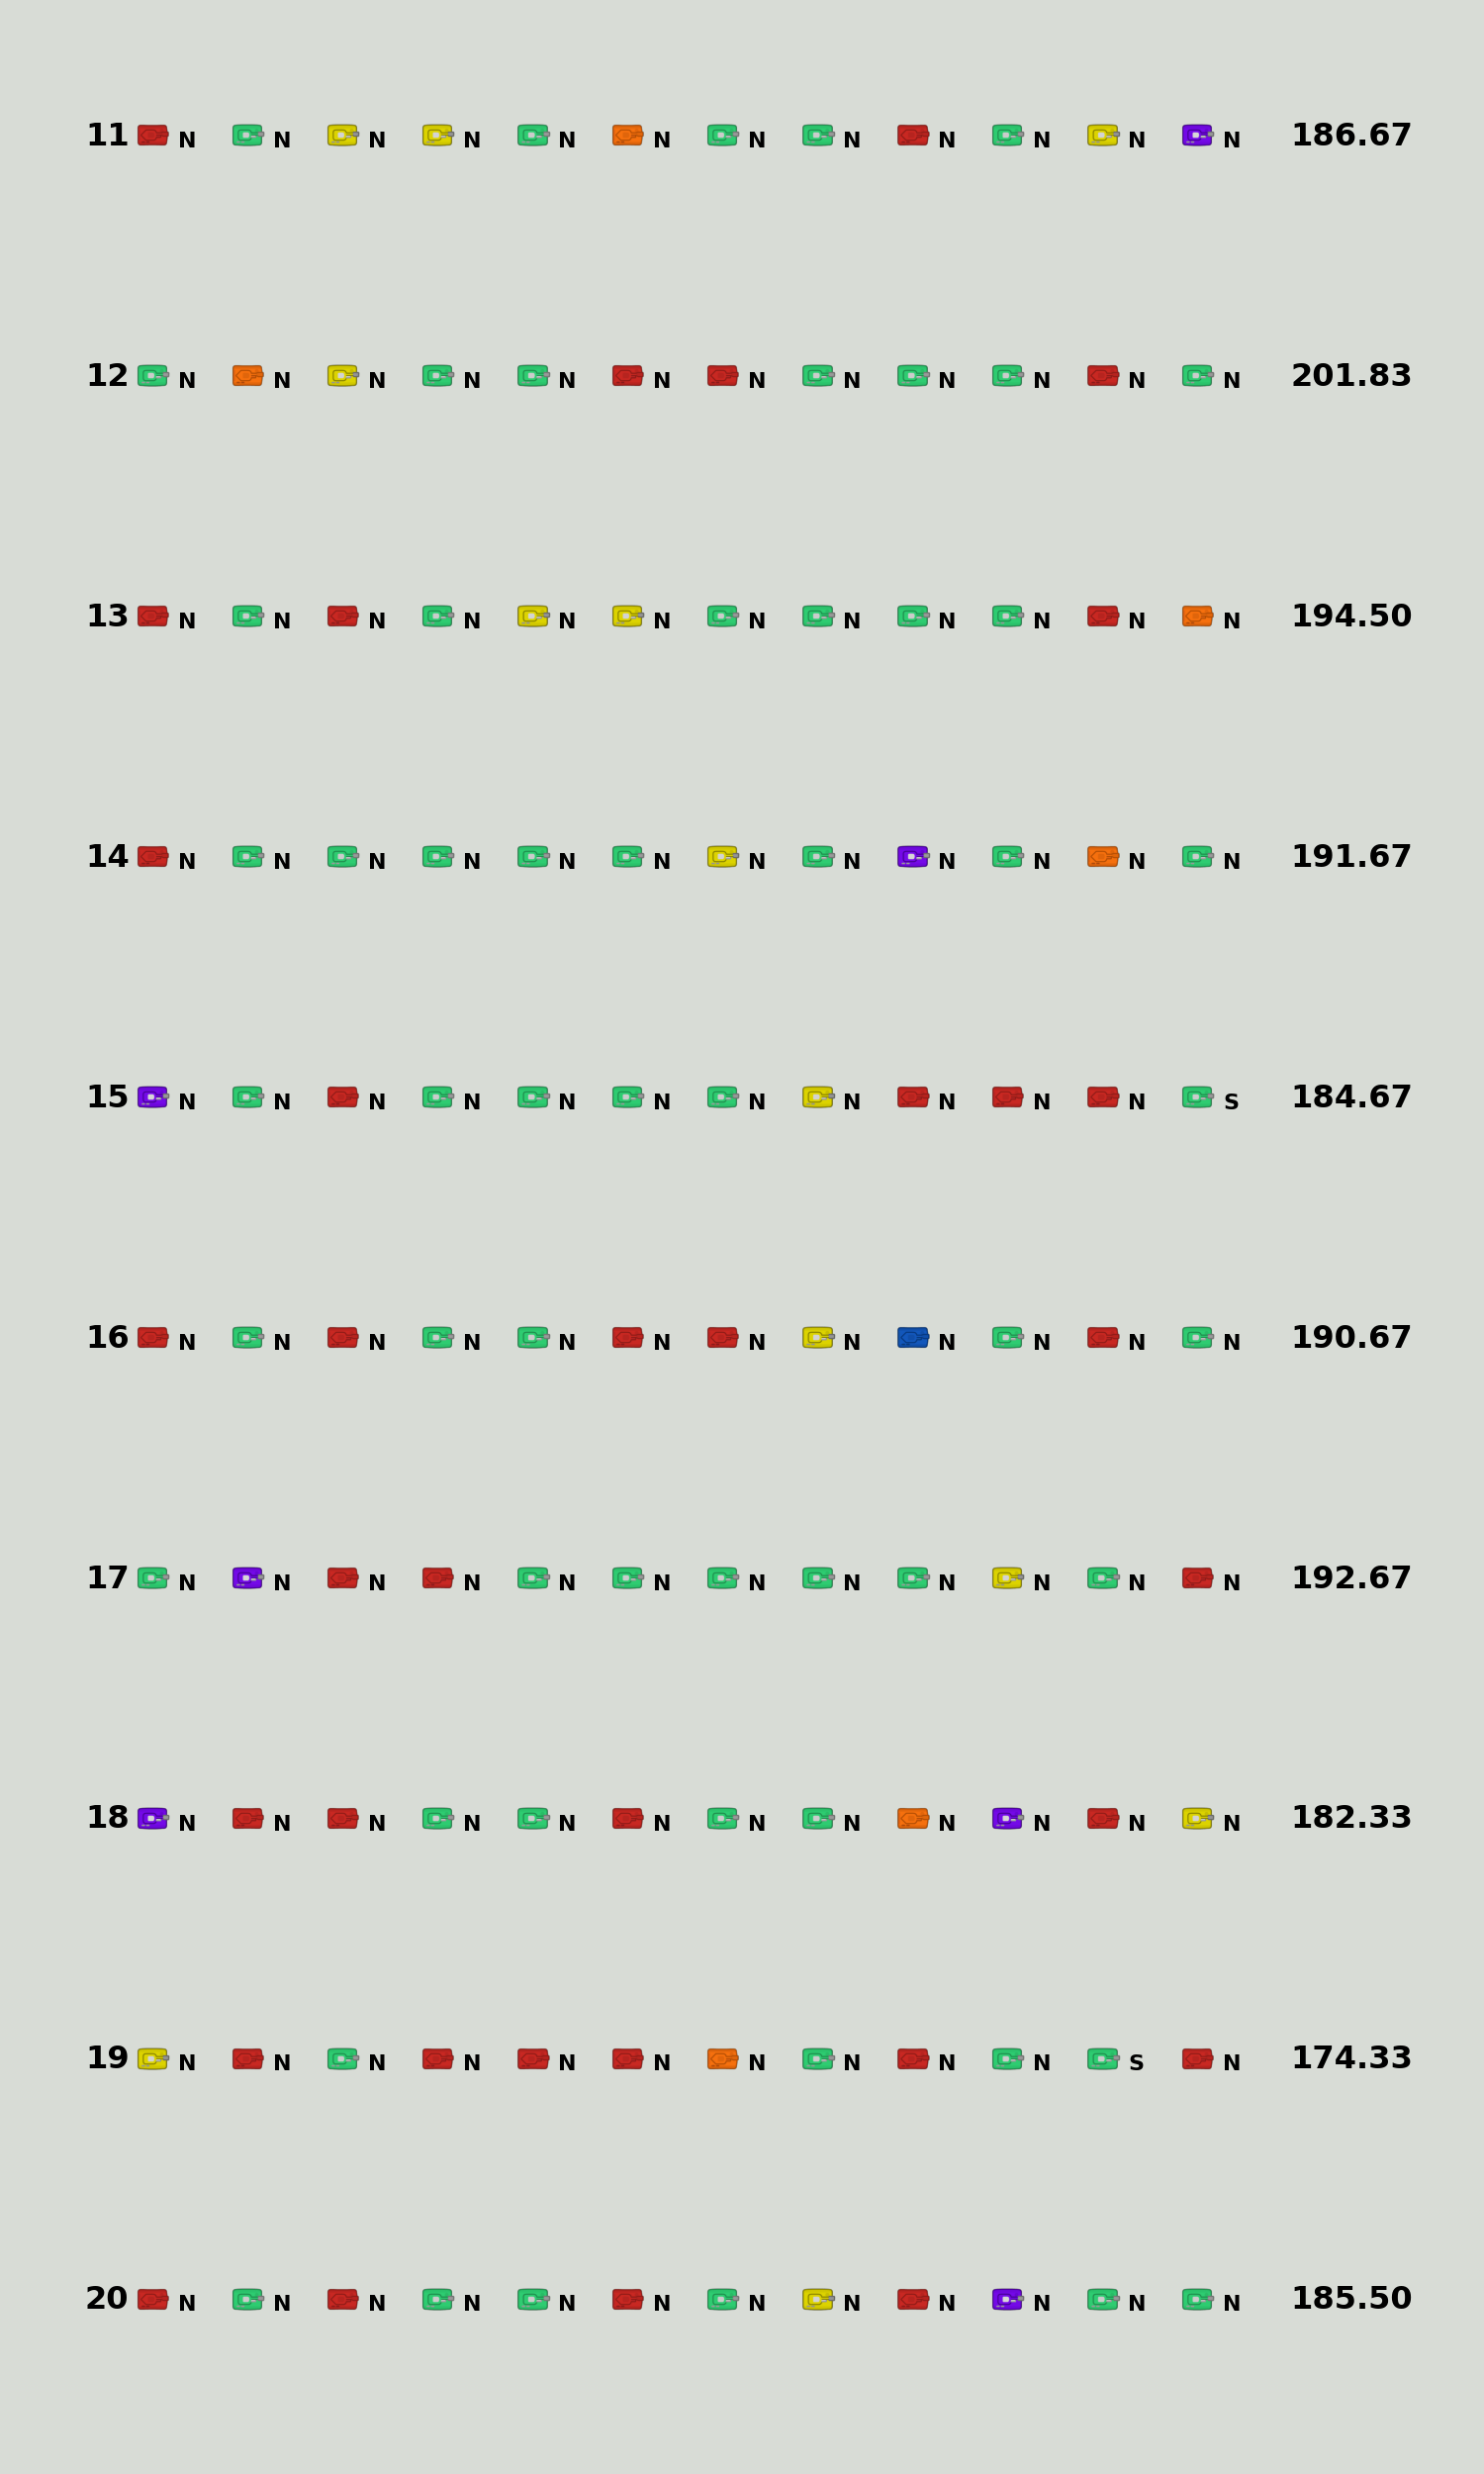
\includegraphics[width=0.9\textwidth]{figuras/td/td_greenred_ai_mode_2_2.png}
  \caption{Visualização da moda de cada onda com a versão v2 contra Torres Verdes + Vermelhas.}
  \label{fig:td-moda-greenred-2-2}
\end{figure}

\begin{figure}[H]
  \centering
  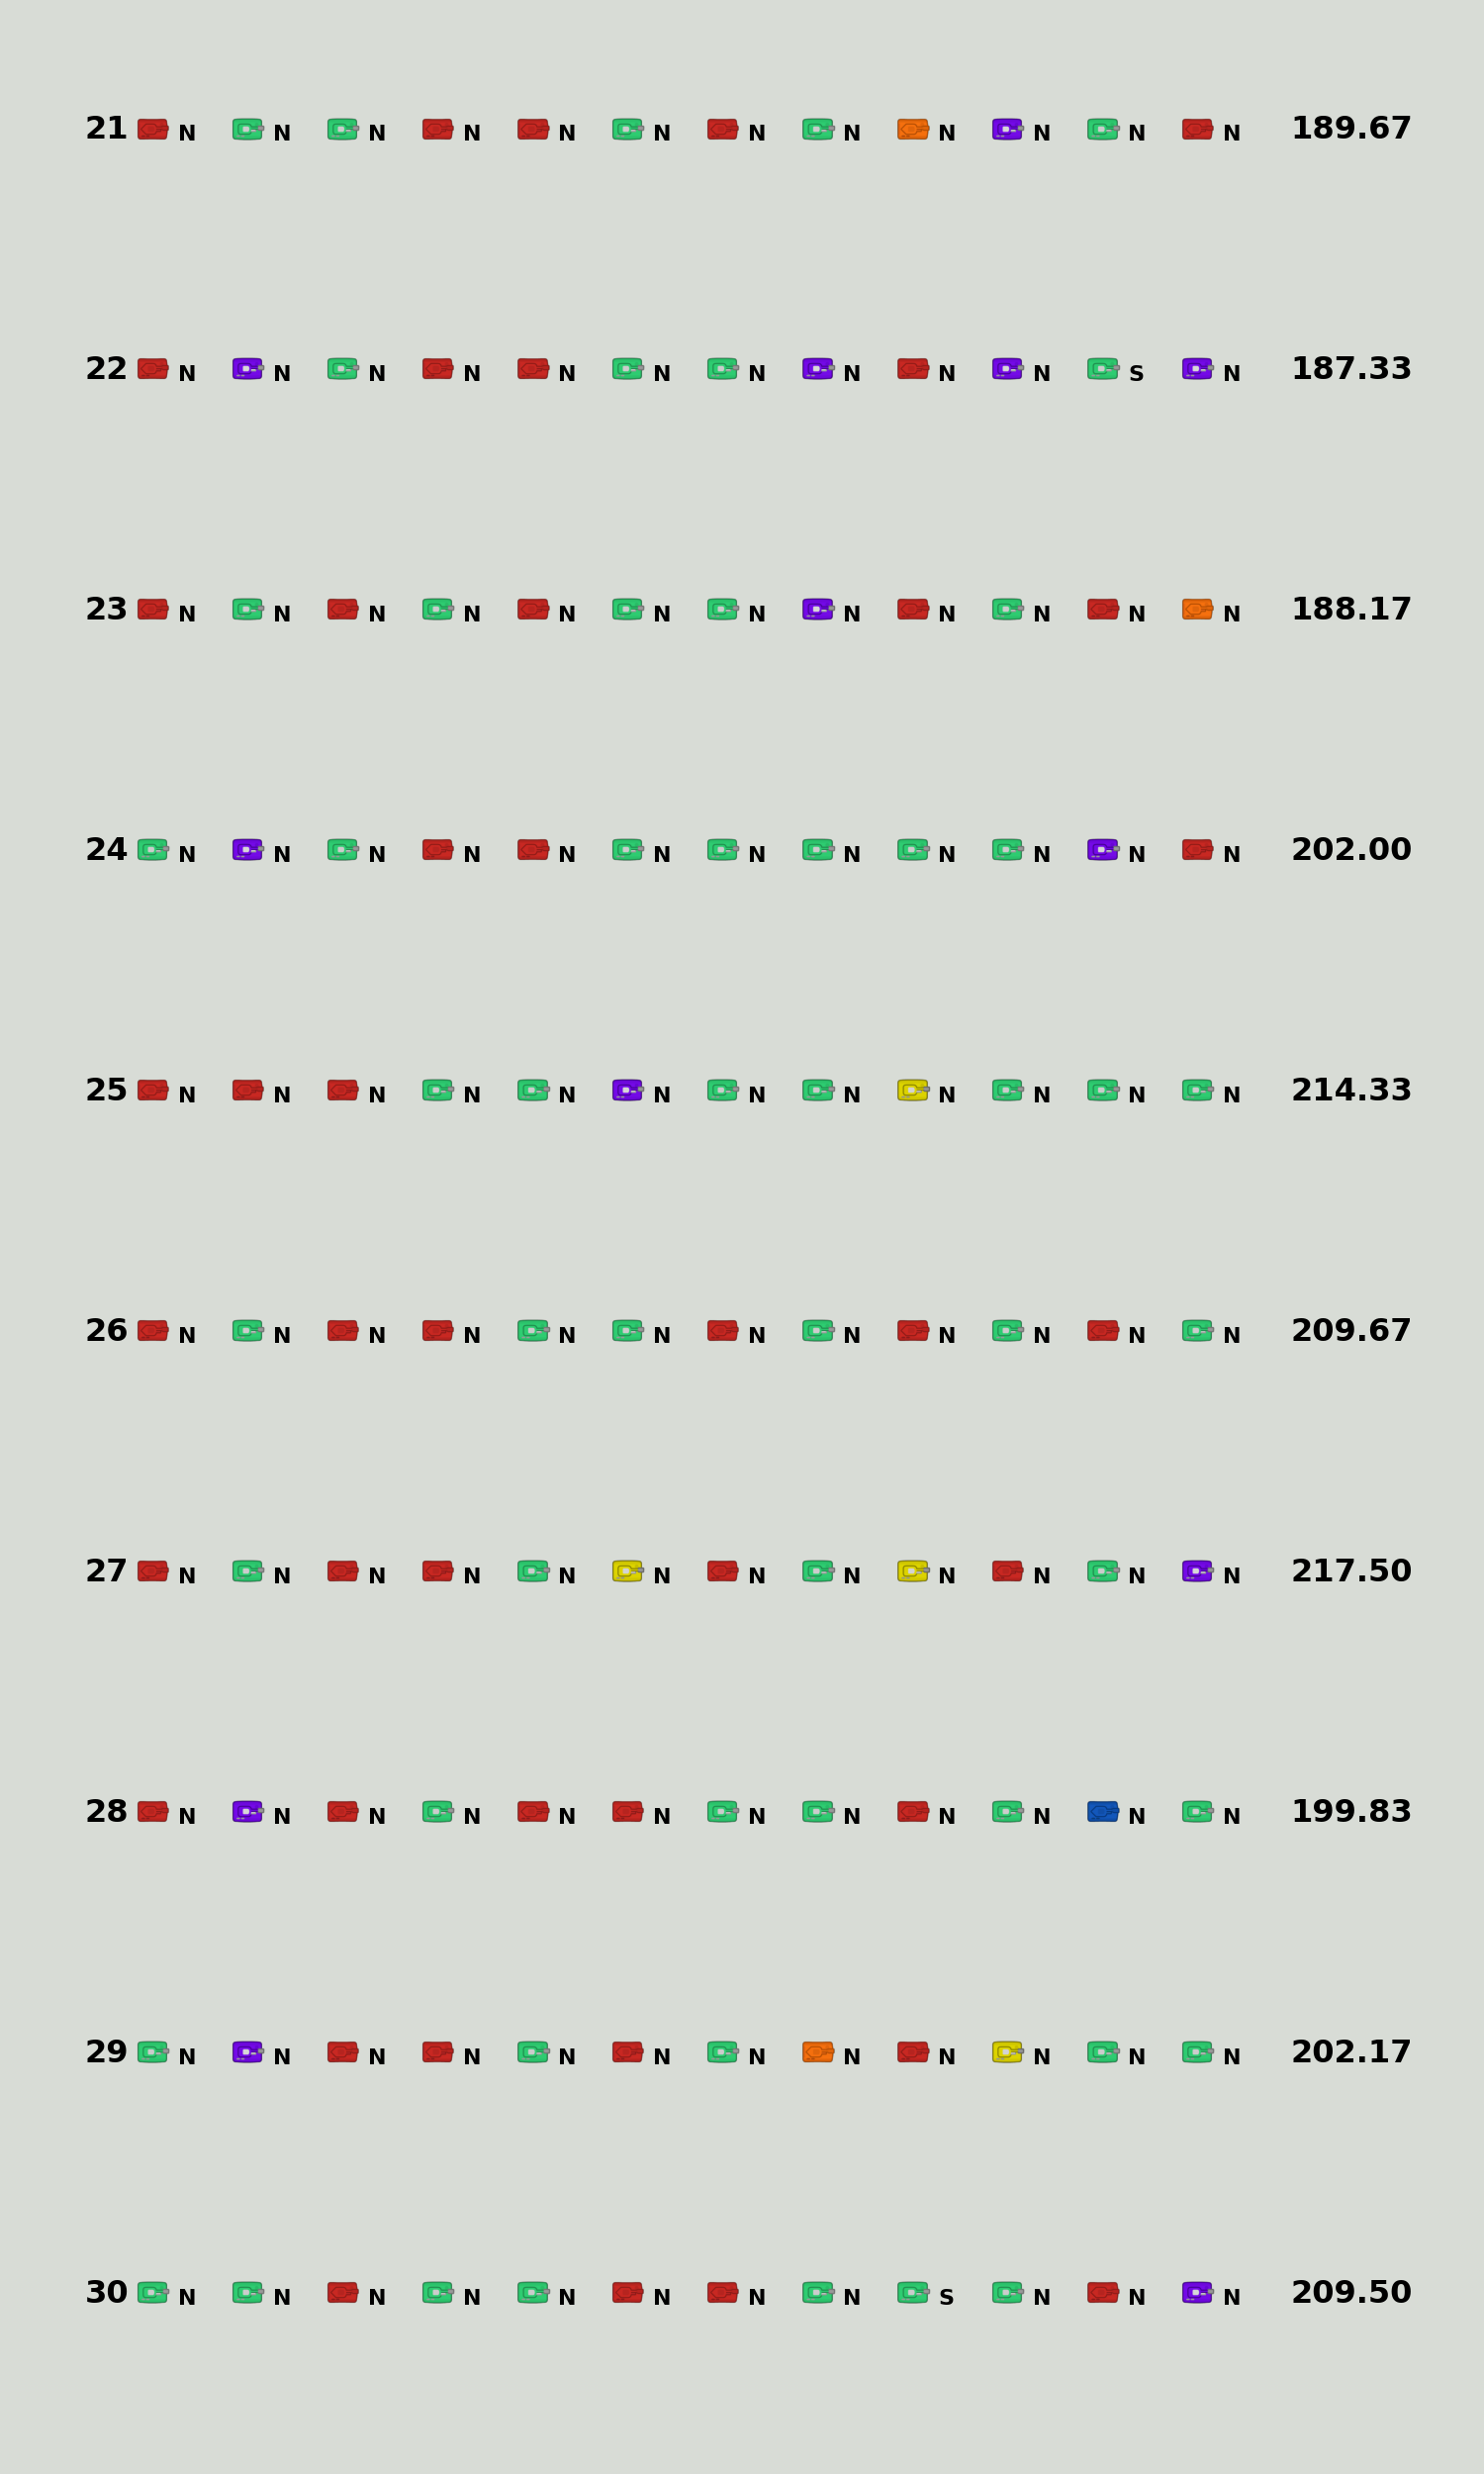
\includegraphics[width=0.9\textwidth]{figuras/td/td_greenred_ai_mode_2_3.png}
  \caption{Visualização da moda de cada onda com a versão v2 contra Torres Verdes + Vermelhas.}
  \label{fig:td-moda-greenred-2-3}
\end{figure}

%% ------------------------------------------------------------------------- %%
\section{Torres Vermelha + Verde}
\label{sec:apend-moda-td-rg-v2}

\begin{figure}[H]
  \centering
  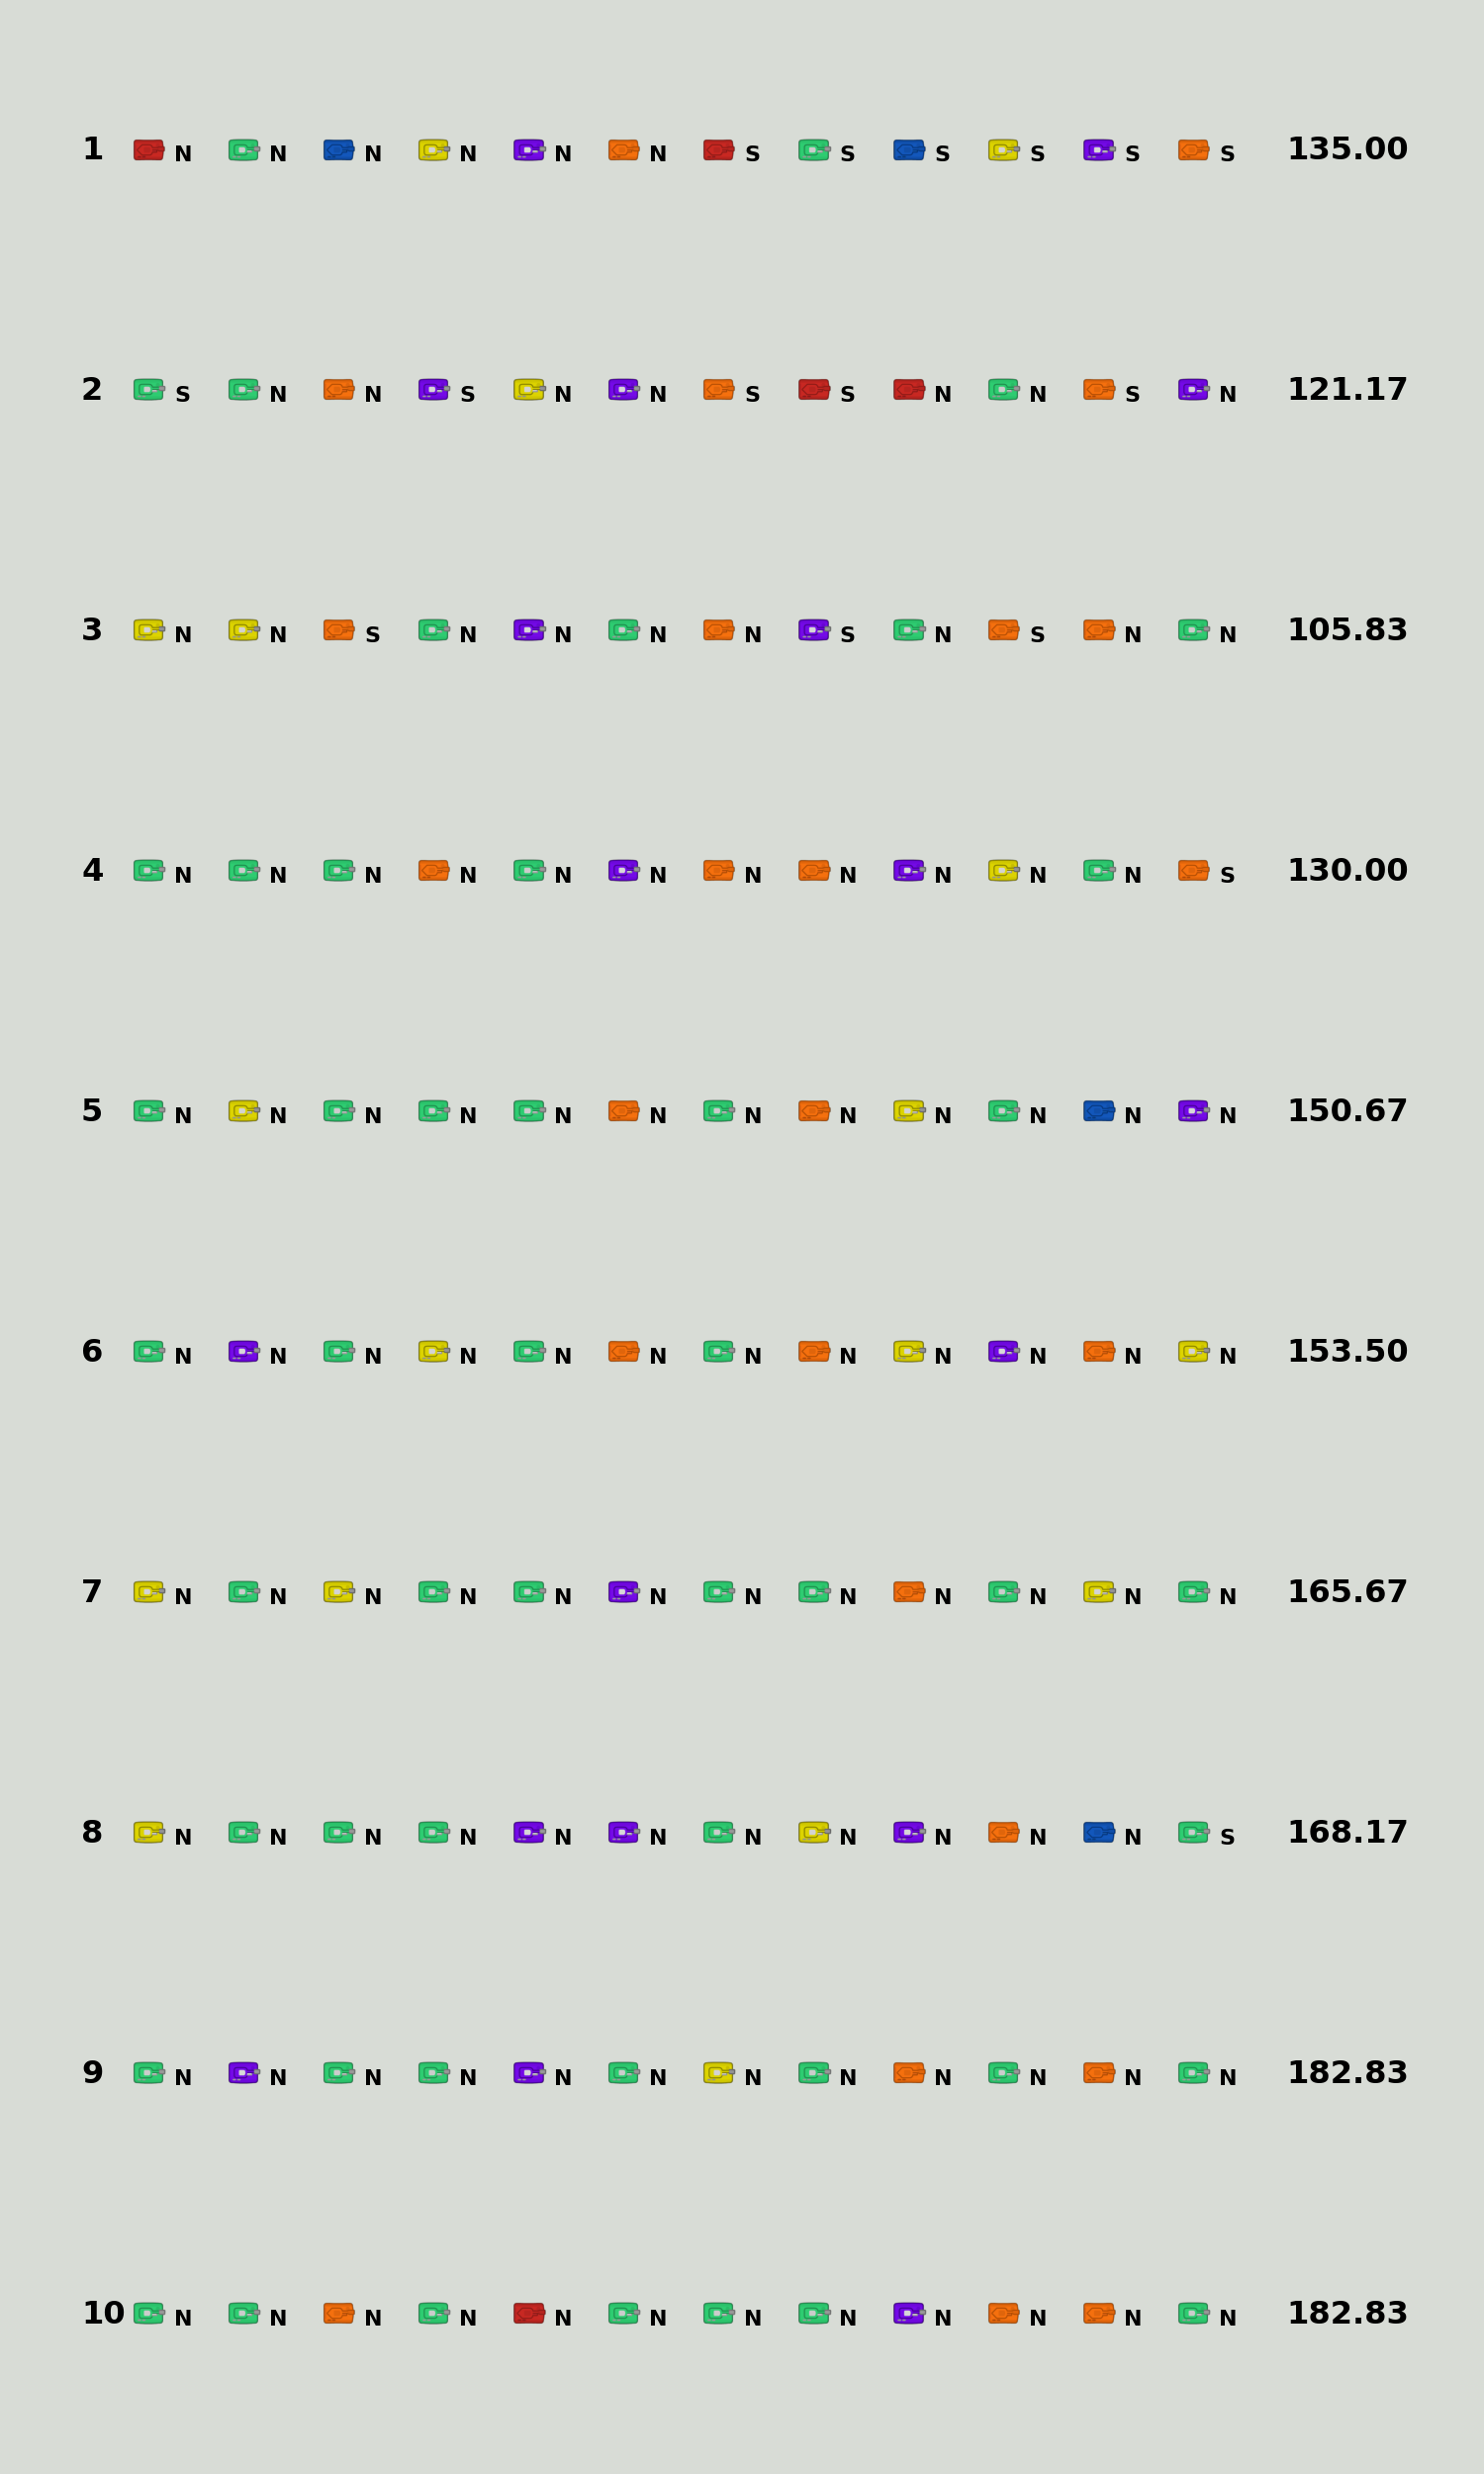
\includegraphics[width=0.9\textwidth]{figuras/td/td_redgreen_ai_mode_2_1.png}
  \caption{Visualização da moda de cada onda com a versão v2 contra Torres Vermelhas + Verdes.}
  \label{fig:td-moda-redgreen-2-1}
\end{figure}

\begin{figure}[H]
  \centering
  \includegraphics[width=0.9\textwidth]{figuras/td/td_redgreen_ai_mode_2_2.png}
  \caption{Visualização da moda de cada onda com a versão v2 contra Torres Vermelhas + Verdes.}
  \label{fig:td-moda-redgreen-2-2}
\end{figure}

\begin{figure}[H]
  \centering
  \includegraphics[width=0.9\textwidth]{figuras/td/td_redgreen_ai_mode_2_3.png}
  \caption{Visualização da moda de cada onda com a versão v2 contra Torres Vermelhas + Verdes.}
  \label{fig:td-moda-redgreen-2-3}
\end{figure}
\par

%% ------------------------------------------------------------------------- %%
\chapter{Moda das Ondas no Tower Defense para a versão v3}
\label{sec:apend-moda-td-v3}

Foram calculadas as modas das ondas do \textit{fitness} desenvolvido, para permitir a visualização dos inimigos mais comuns que o algoritmo convergiu.

%% ------------------------------------------------------------------------- %%
\section{Torres Verdes}
\label{sec:apend-moda-td-g-v3}

\begin{figure}[H]
  \centering
  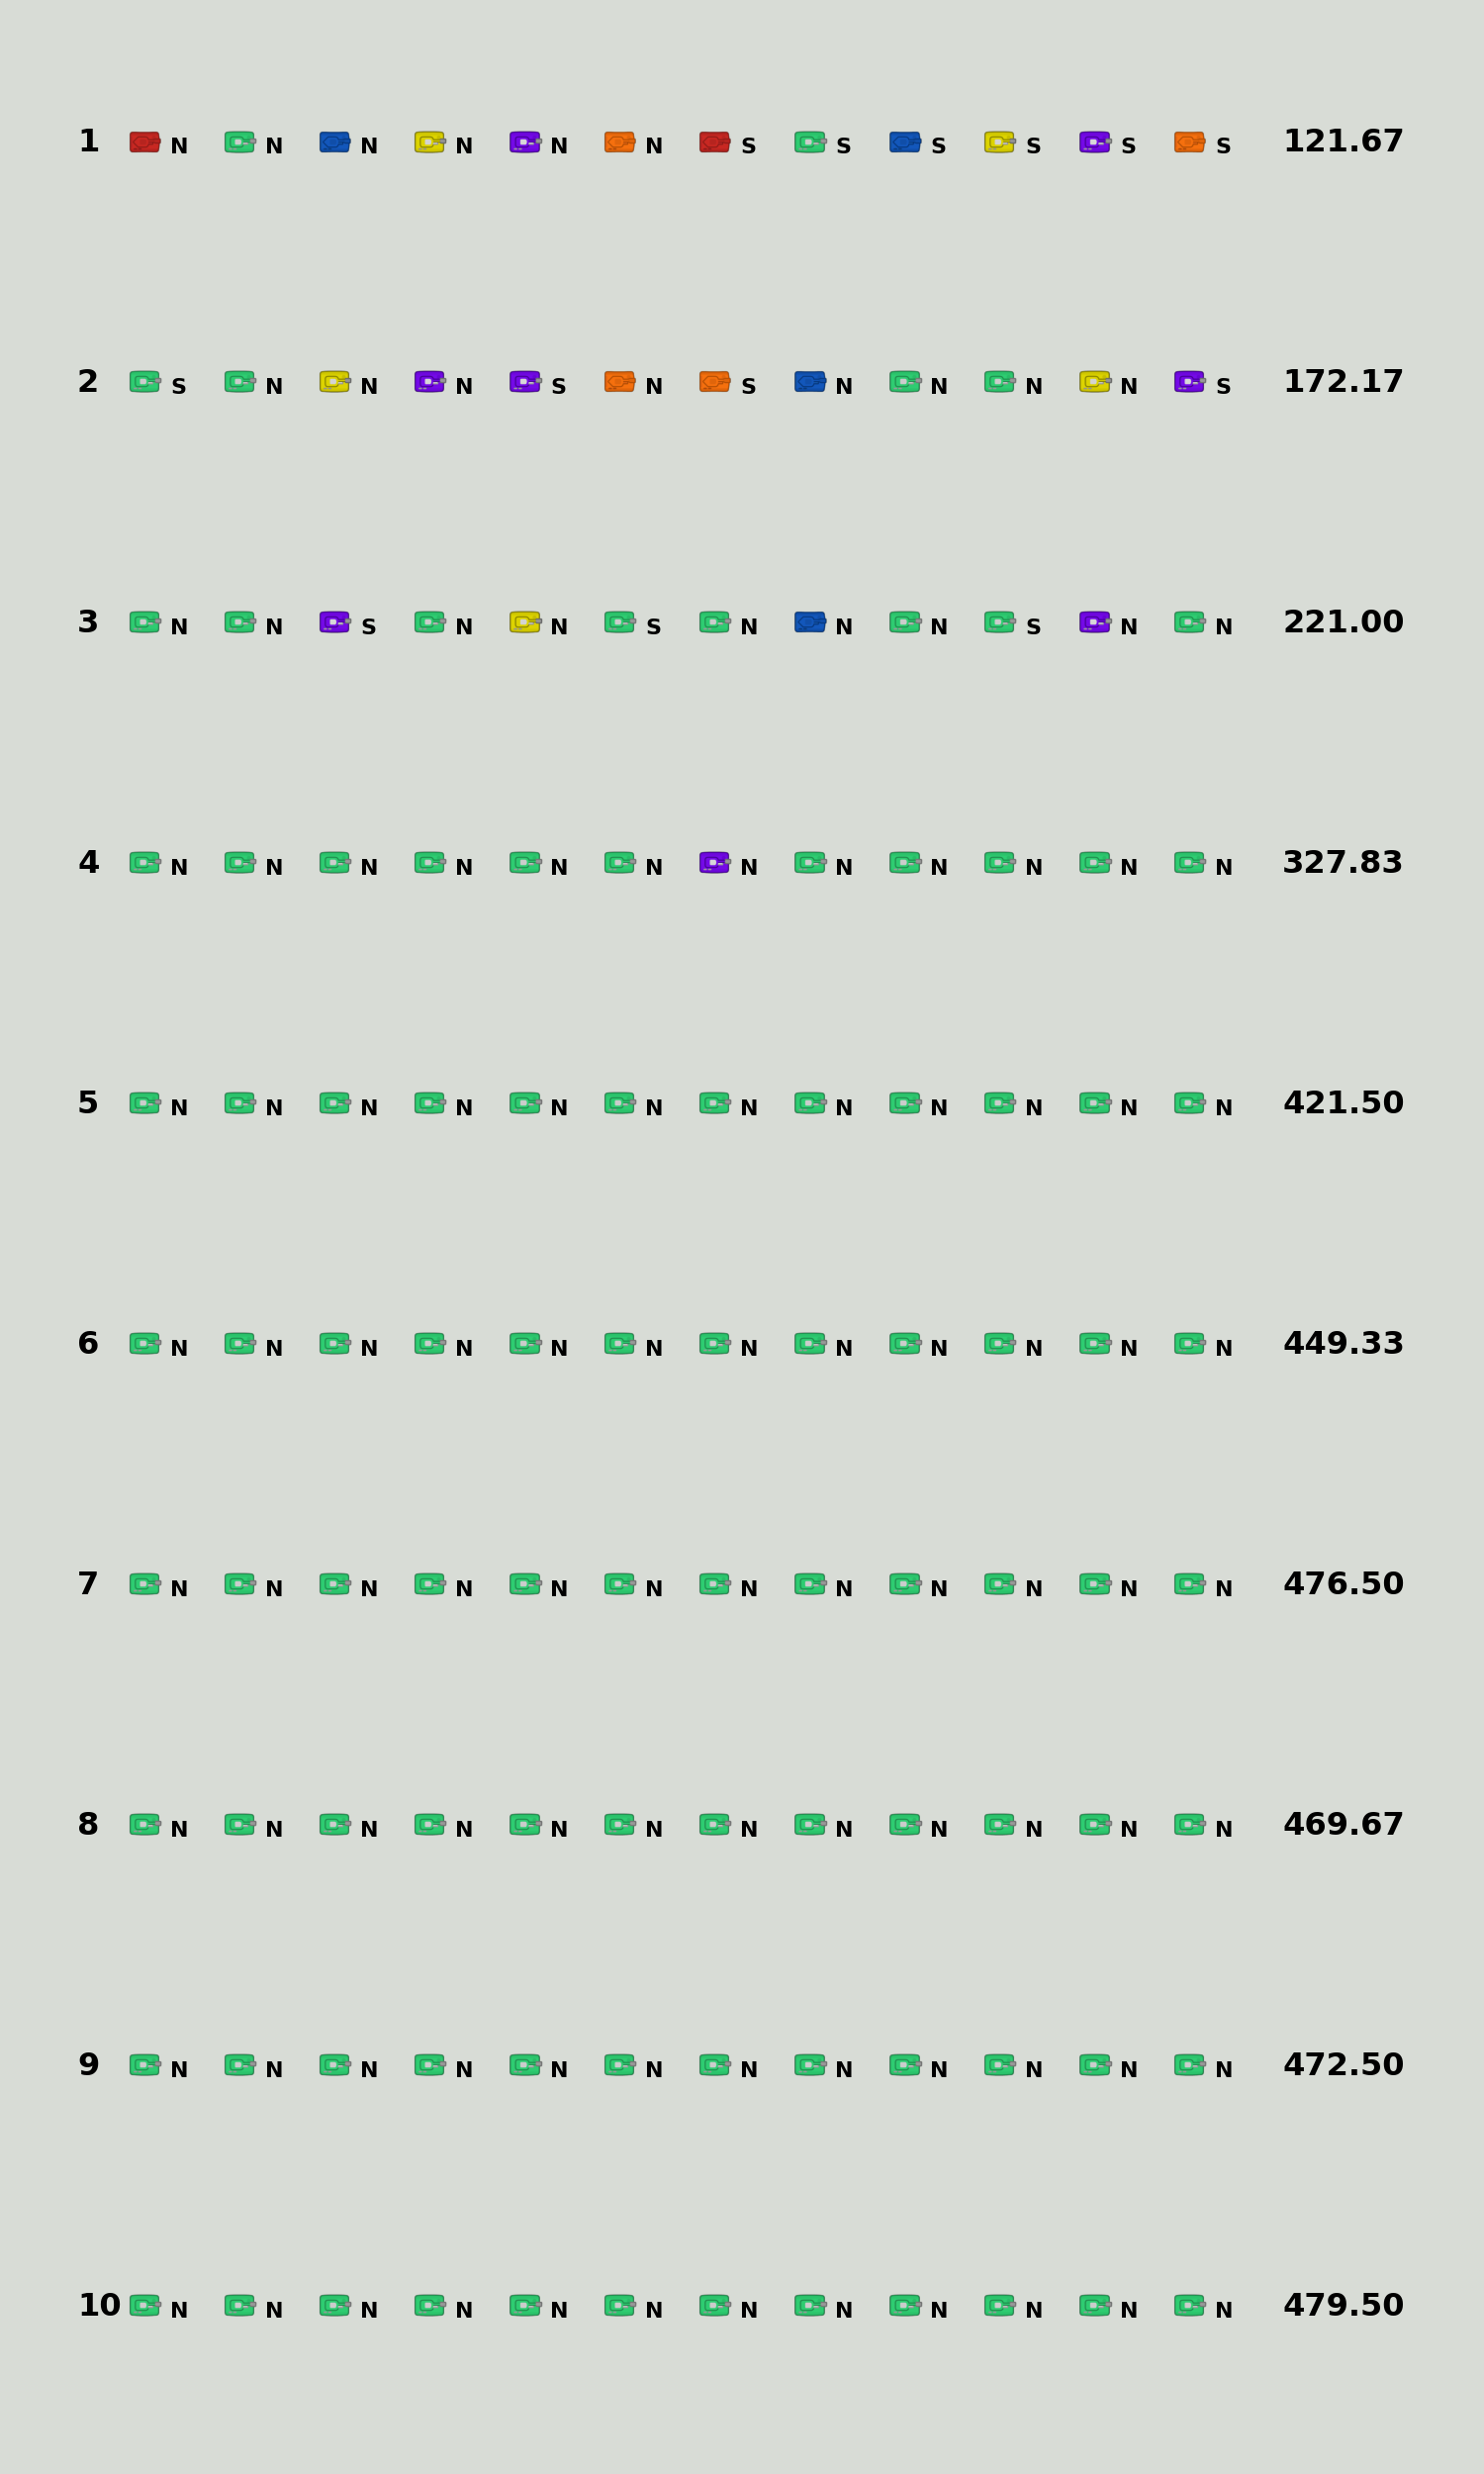
\includegraphics[width=0.9\textwidth]{figuras/td/td_allgreen_ai_mode_3_1.png}
  \caption{Visualização da moda de cada onda com a versão v3 contra Torres Verdes.}
  \label{fig:td-moda-green-3-1}
\end{figure}

\begin{figure}[H]
  \centering
  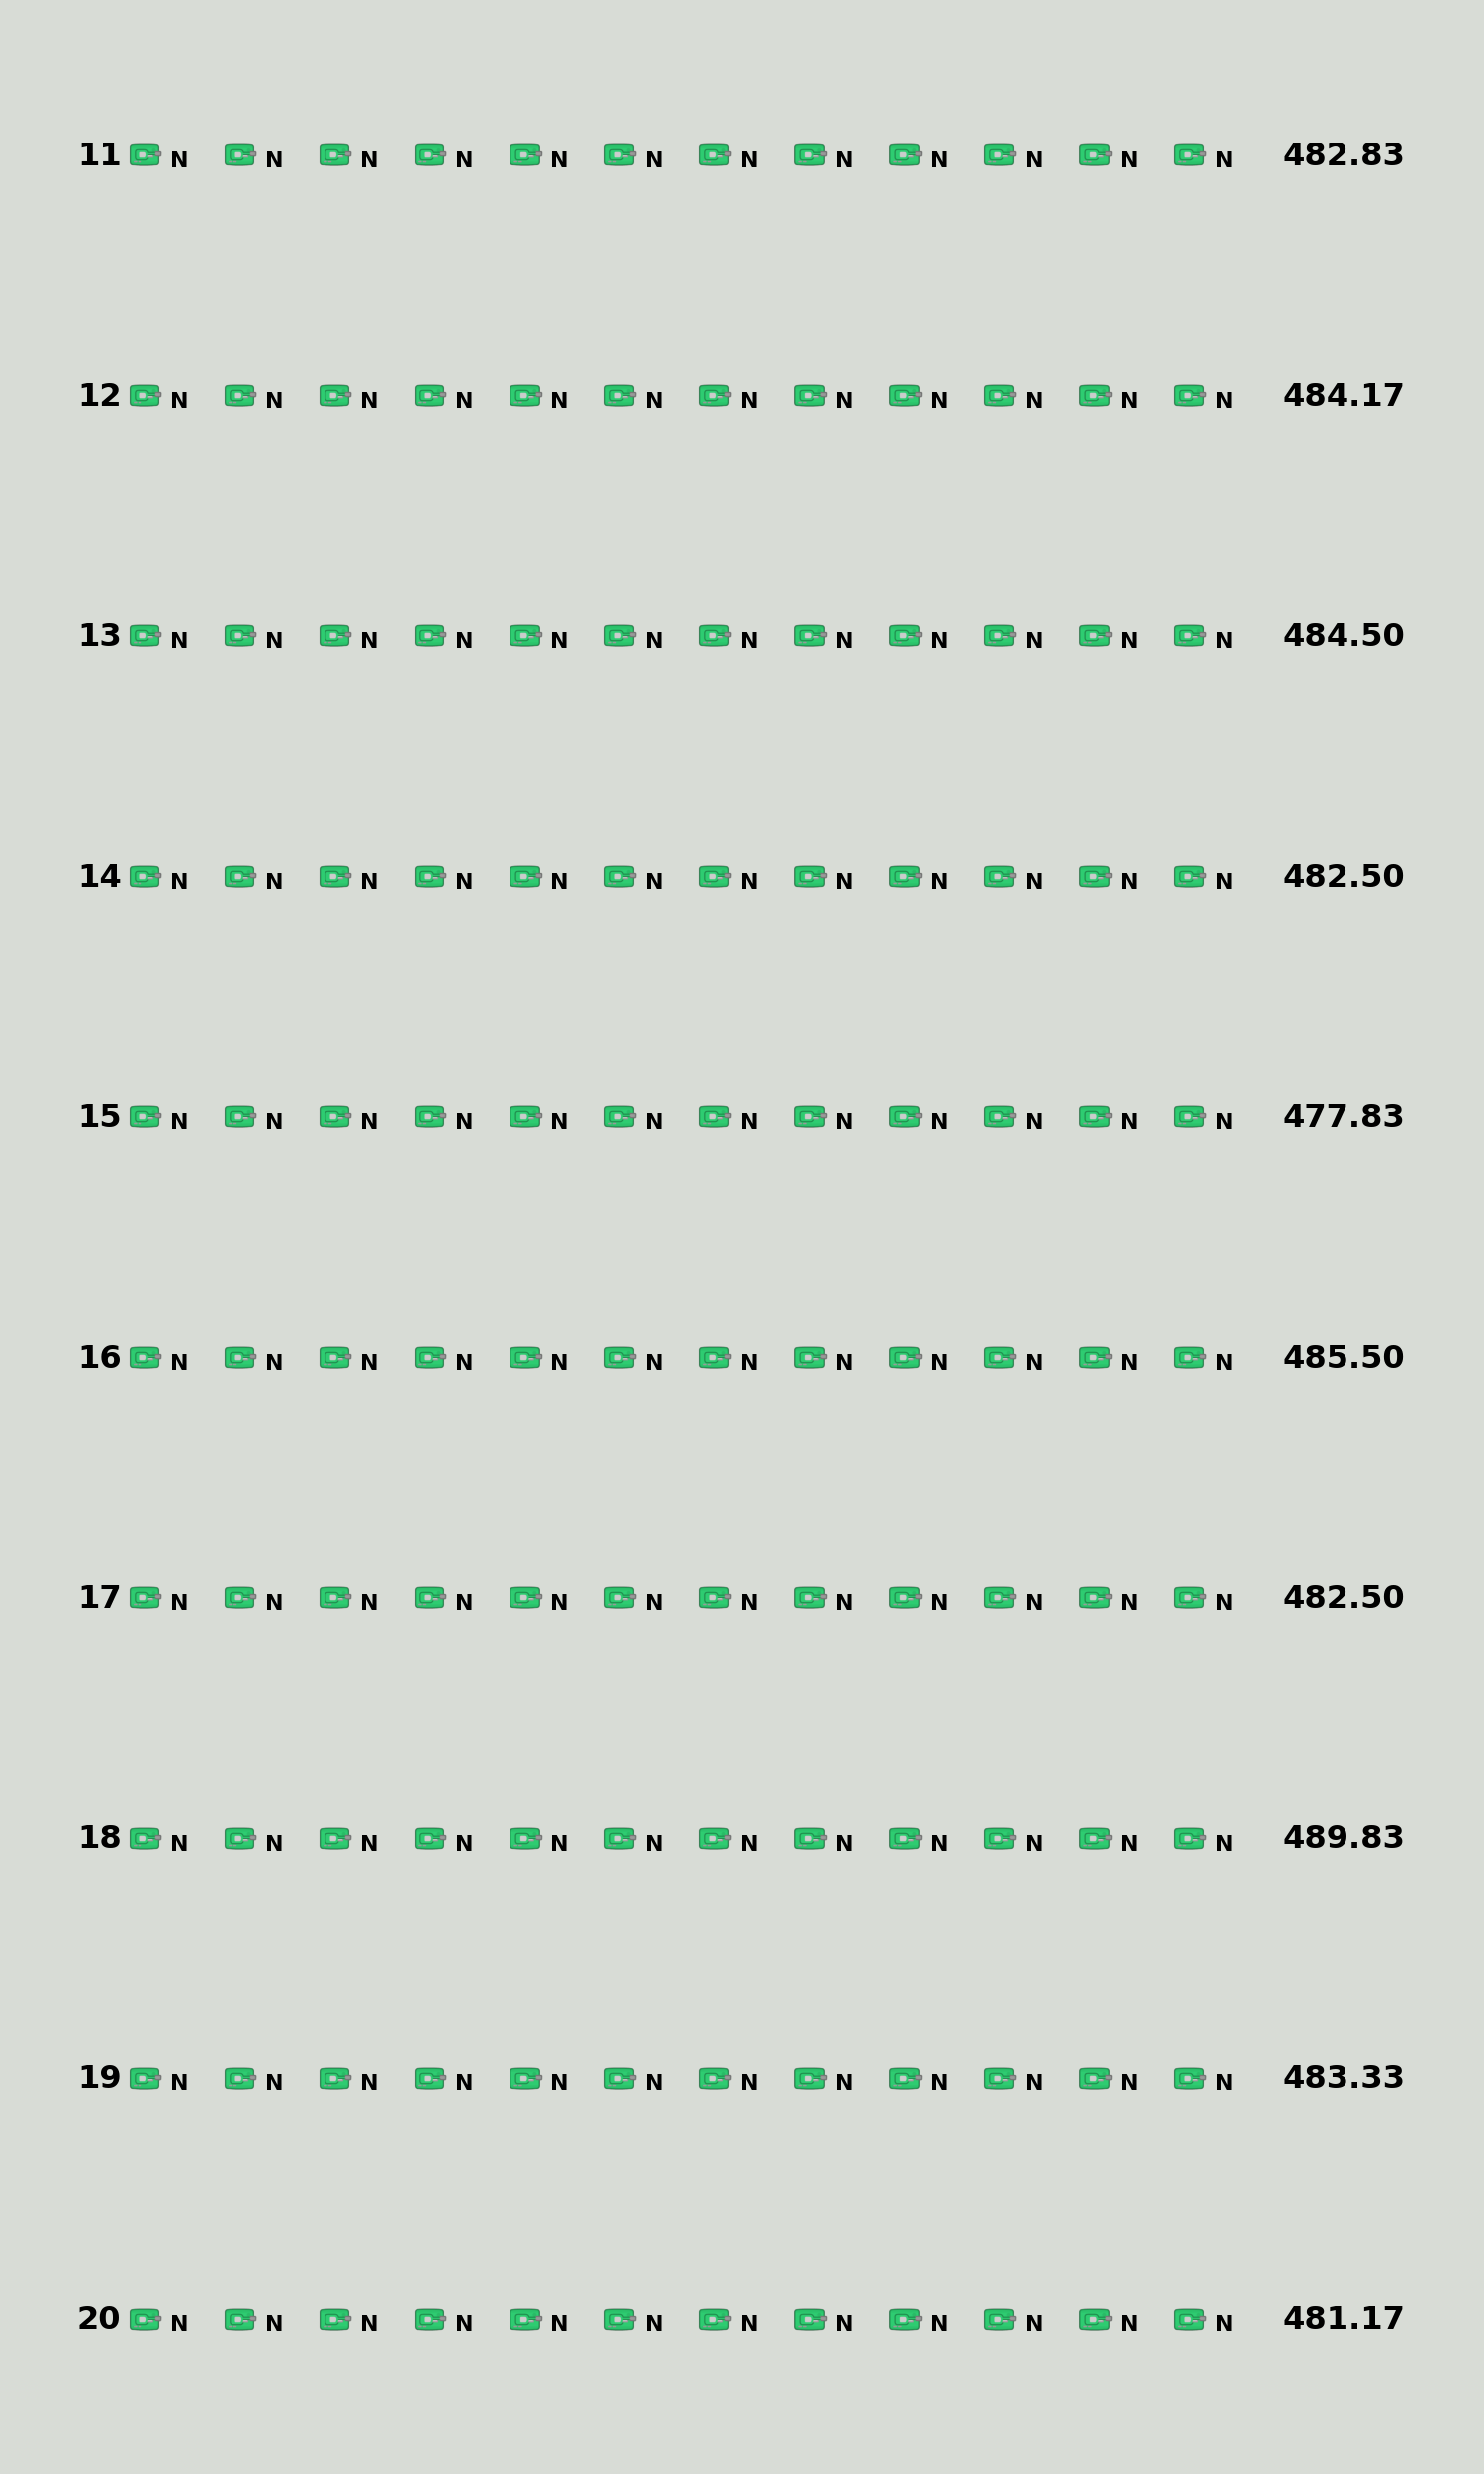
\includegraphics[width=0.9\textwidth]{figuras/td/td_allgreen_ai_mode_3_2.png}
  \caption{Visualização da moda de cada onda com a versão v3 contra Torres Verdes.}
  \label{fig:td-moda-green-3-2}
\end{figure}

\begin{figure}[H]
  \centering
  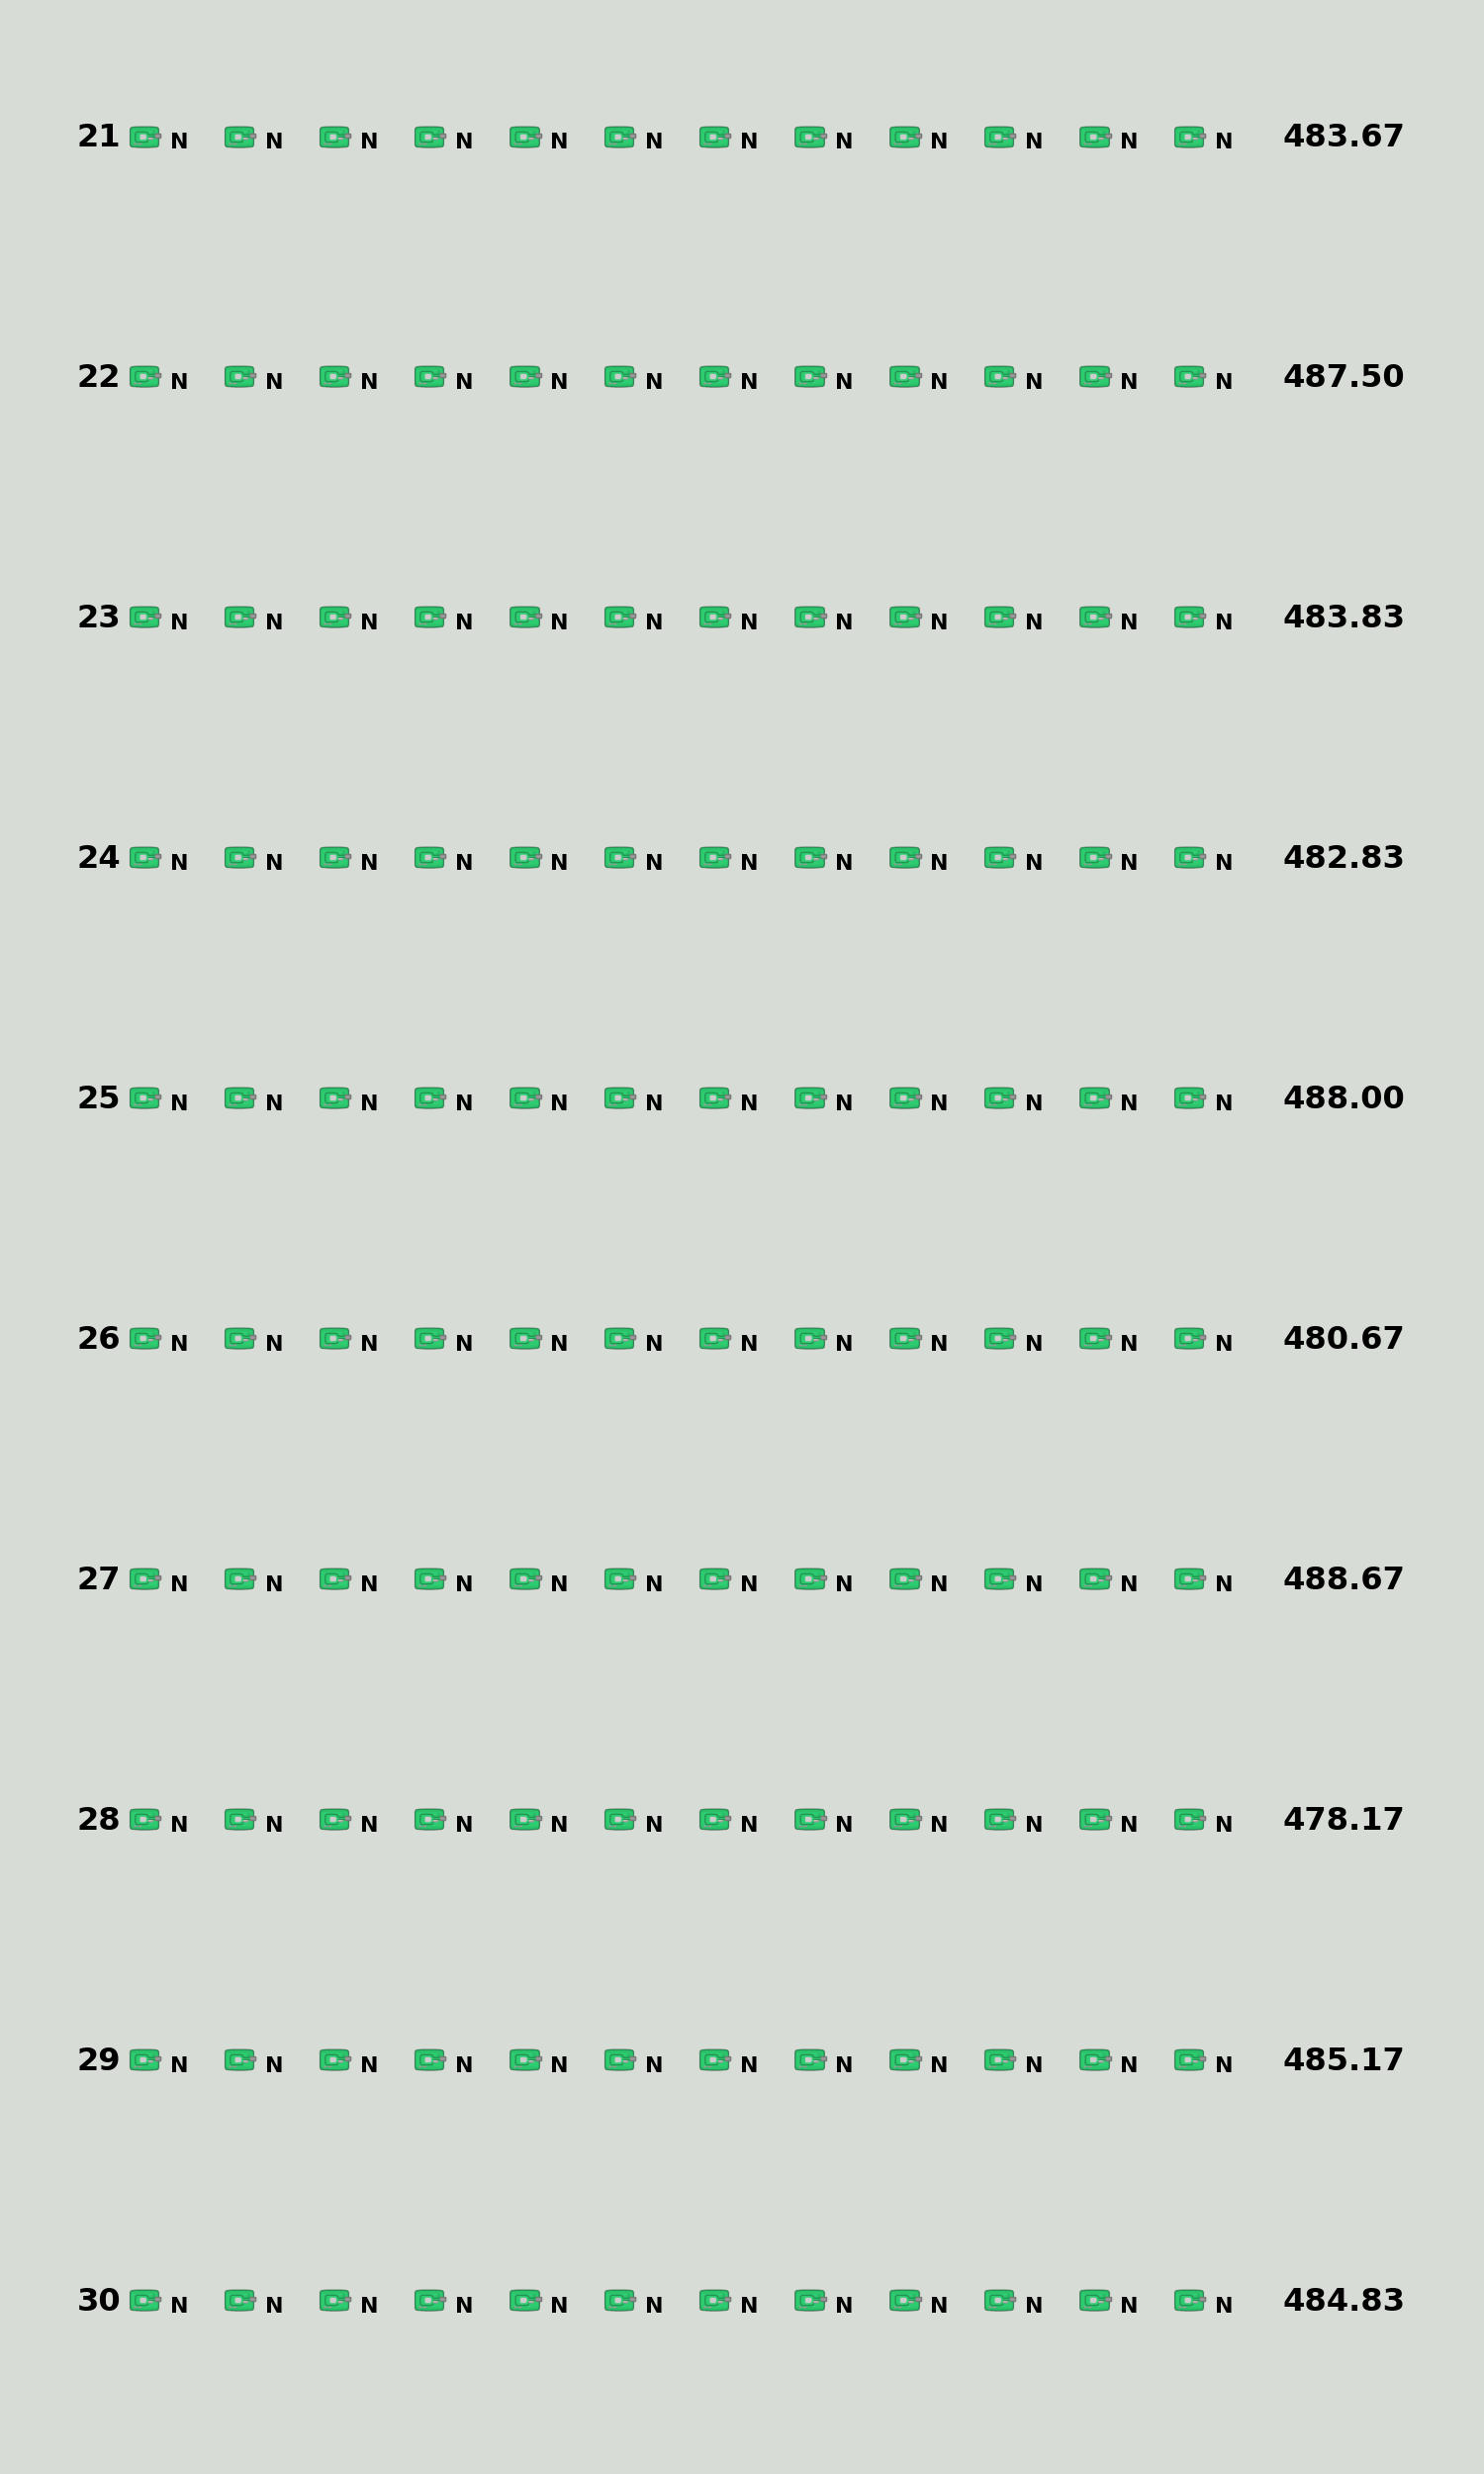
\includegraphics[width=0.9\textwidth]{figuras/td/td_allgreen_ai_mode_3_3.png}
  \caption{Visualização da moda de cada onda com a versão v3 contra Torres Verdes.}
  \label{fig:td-moda-green-3-3}
\end{figure}

%% ------------------------------------------------------------------------- %%
\section{Torres Vermelhas}
\label{sec:apend-moda-td-r-v3}

\begin{figure}[H]
  \centering
  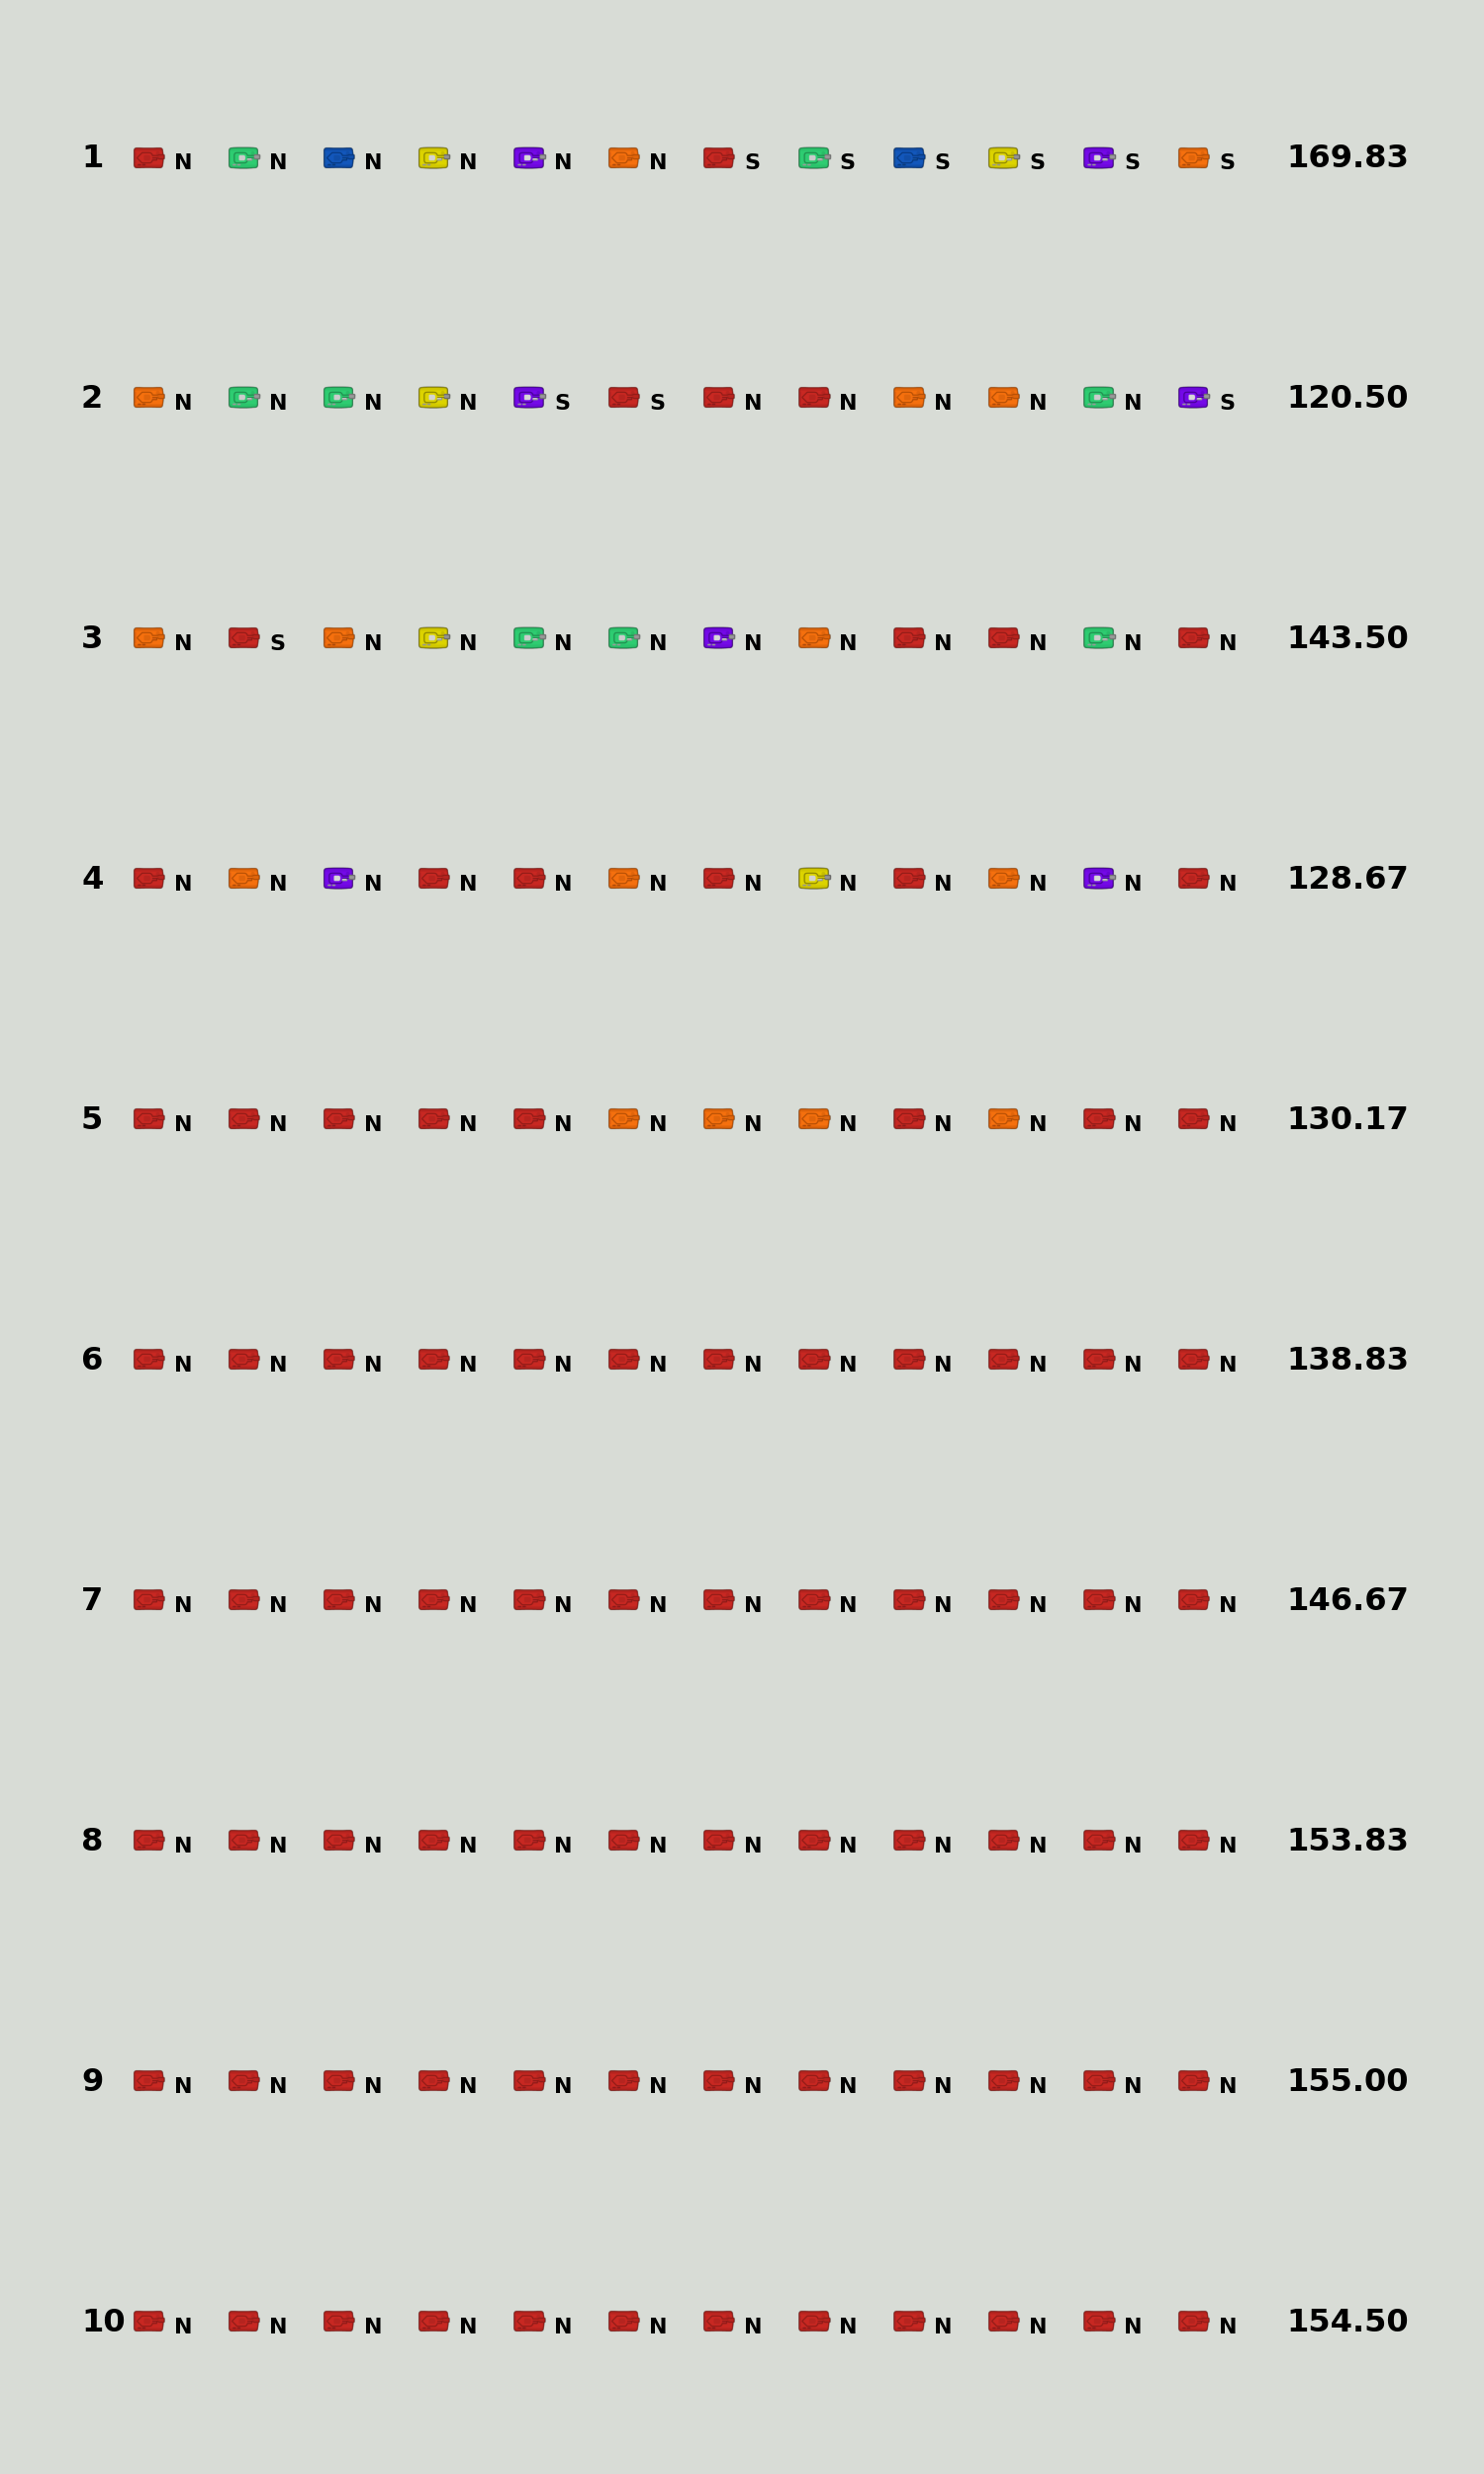
\includegraphics[width=0.9\textwidth]{figuras/td/td_allred_ai_mode_3_1.png}
  \caption{Visualização da moda de cada onda com a versão v3 contra Torres Vermelhas.}
  \label{fig:td-moda-red-3-1}
\end{figure}

\begin{figure}[H]
  \centering
  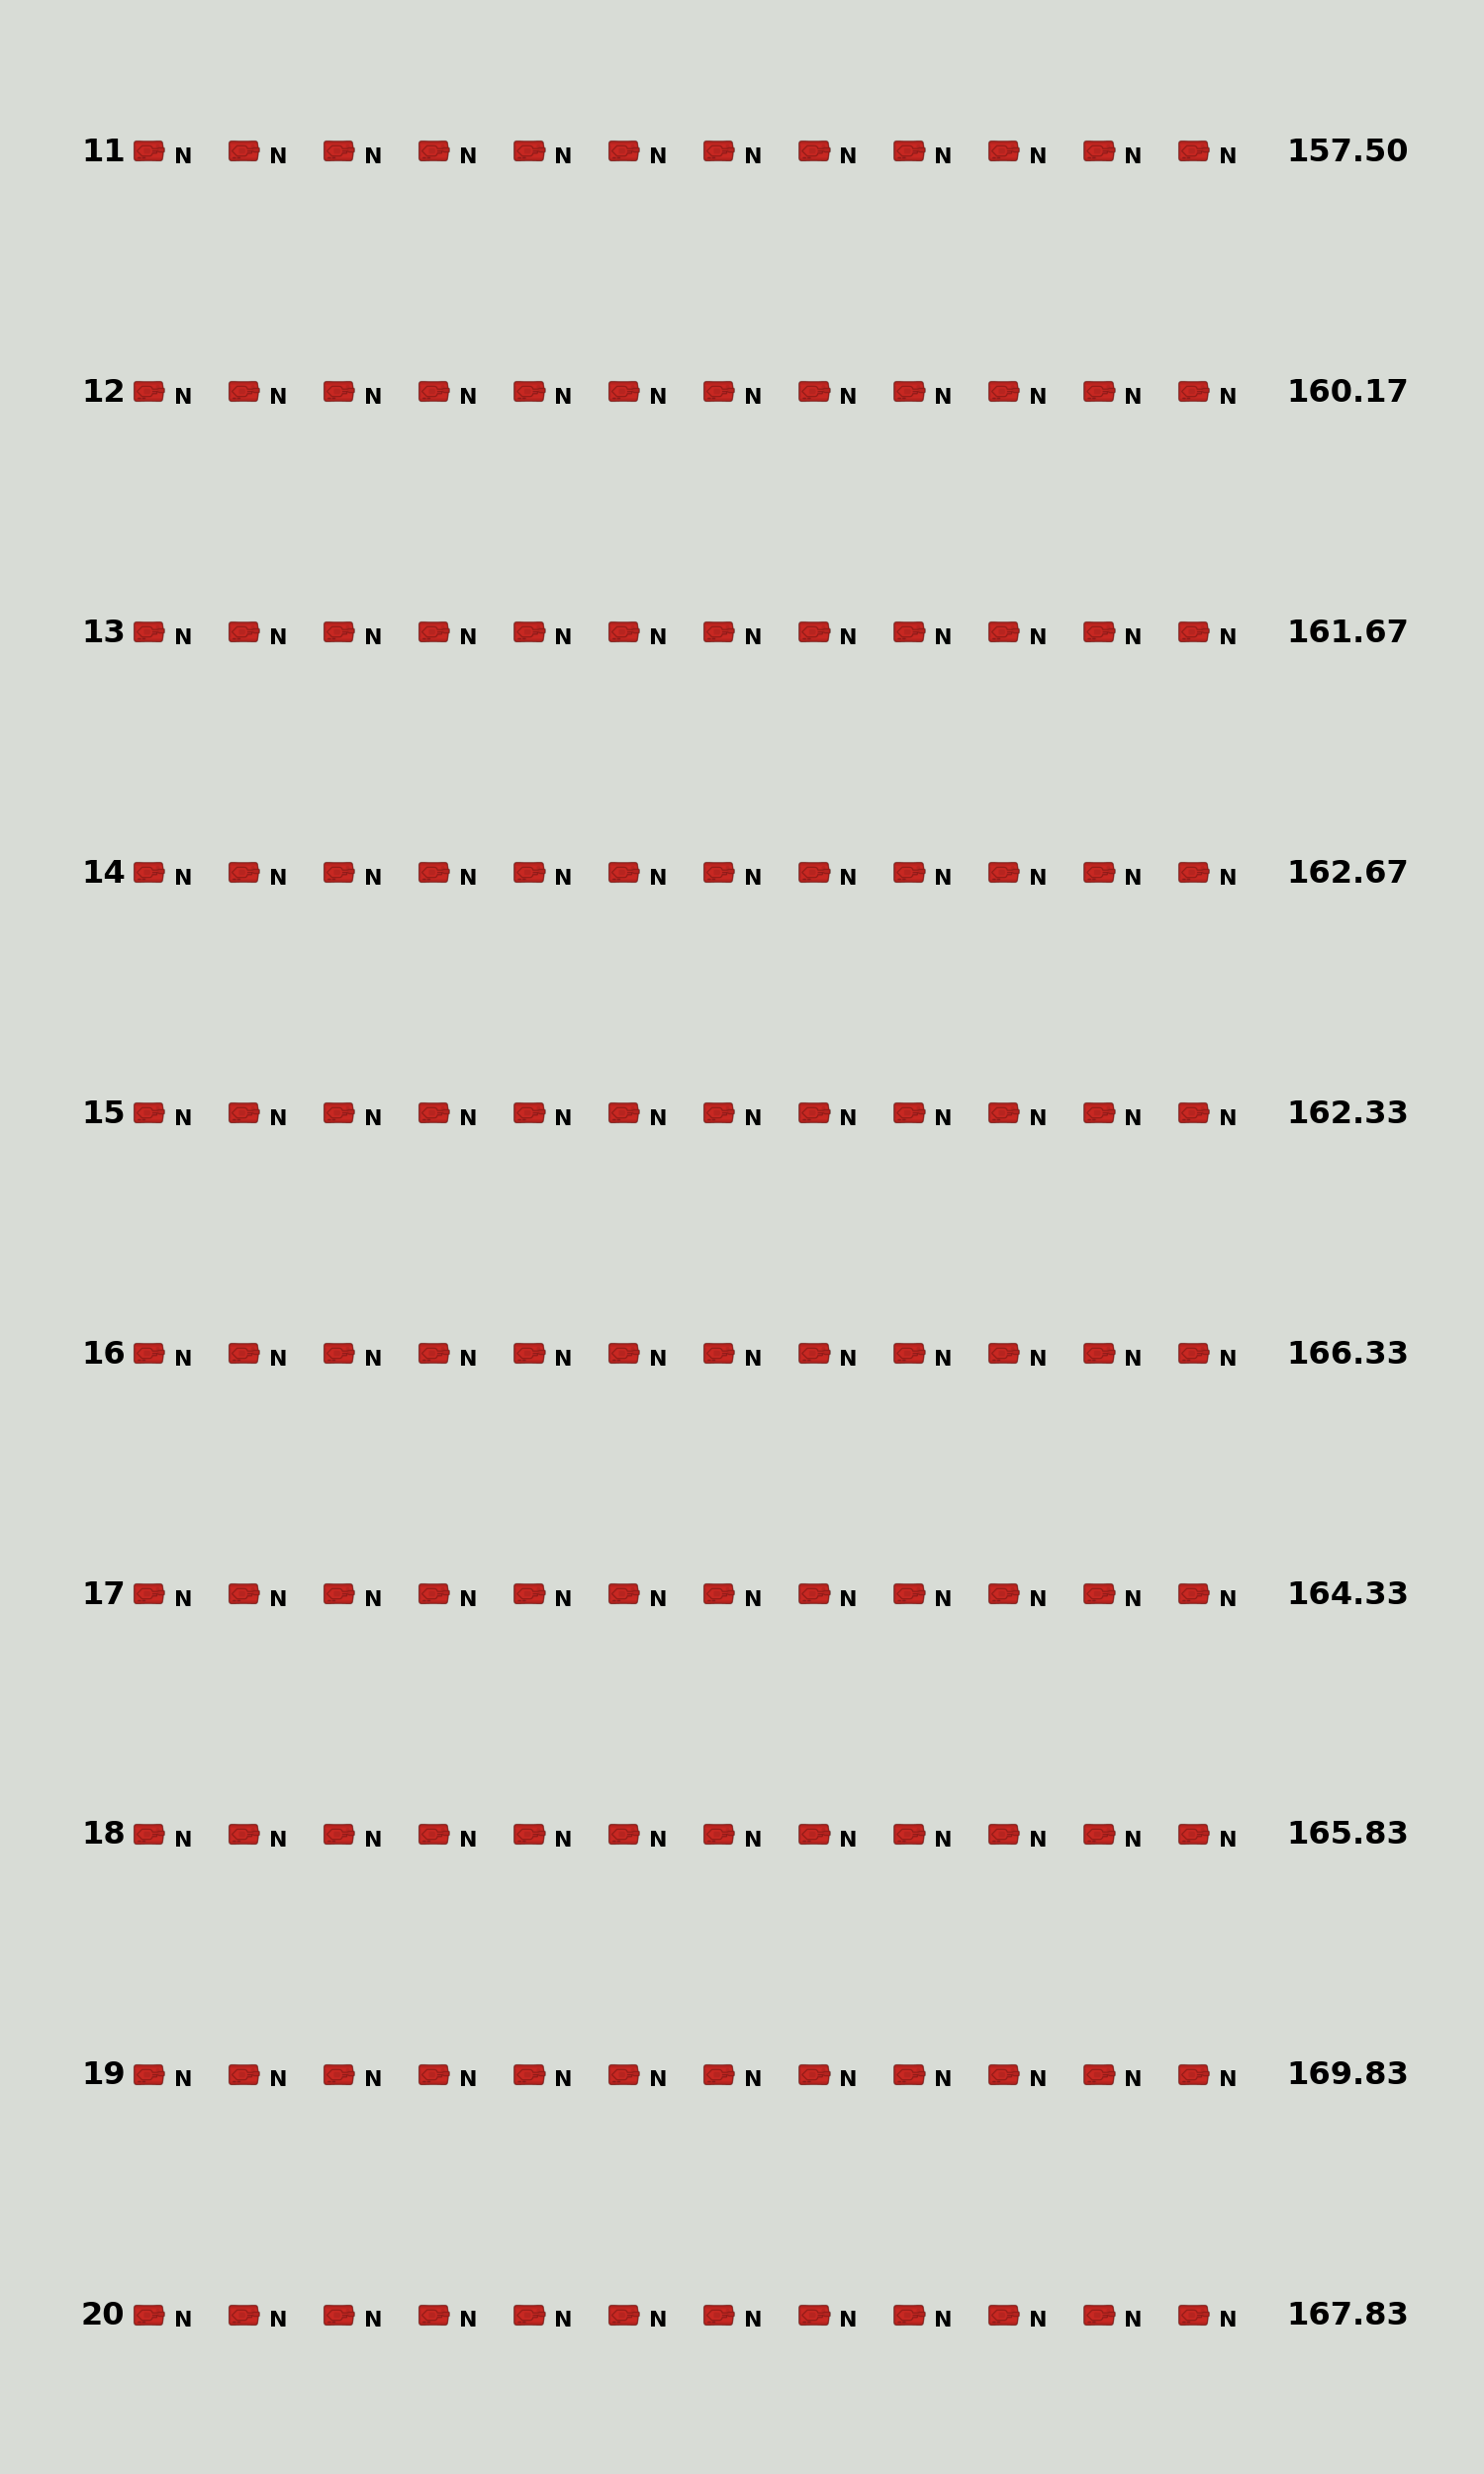
\includegraphics[width=0.9\textwidth]{figuras/td/td_allred_ai_mode_3_2.png}
  \caption{Visualização da moda de cada onda com a versão v3 contra Torres Vermelhas.}
  \label{fig:td-moda-red-3-2}
\end{figure}

\begin{figure}[H]
  \centering
  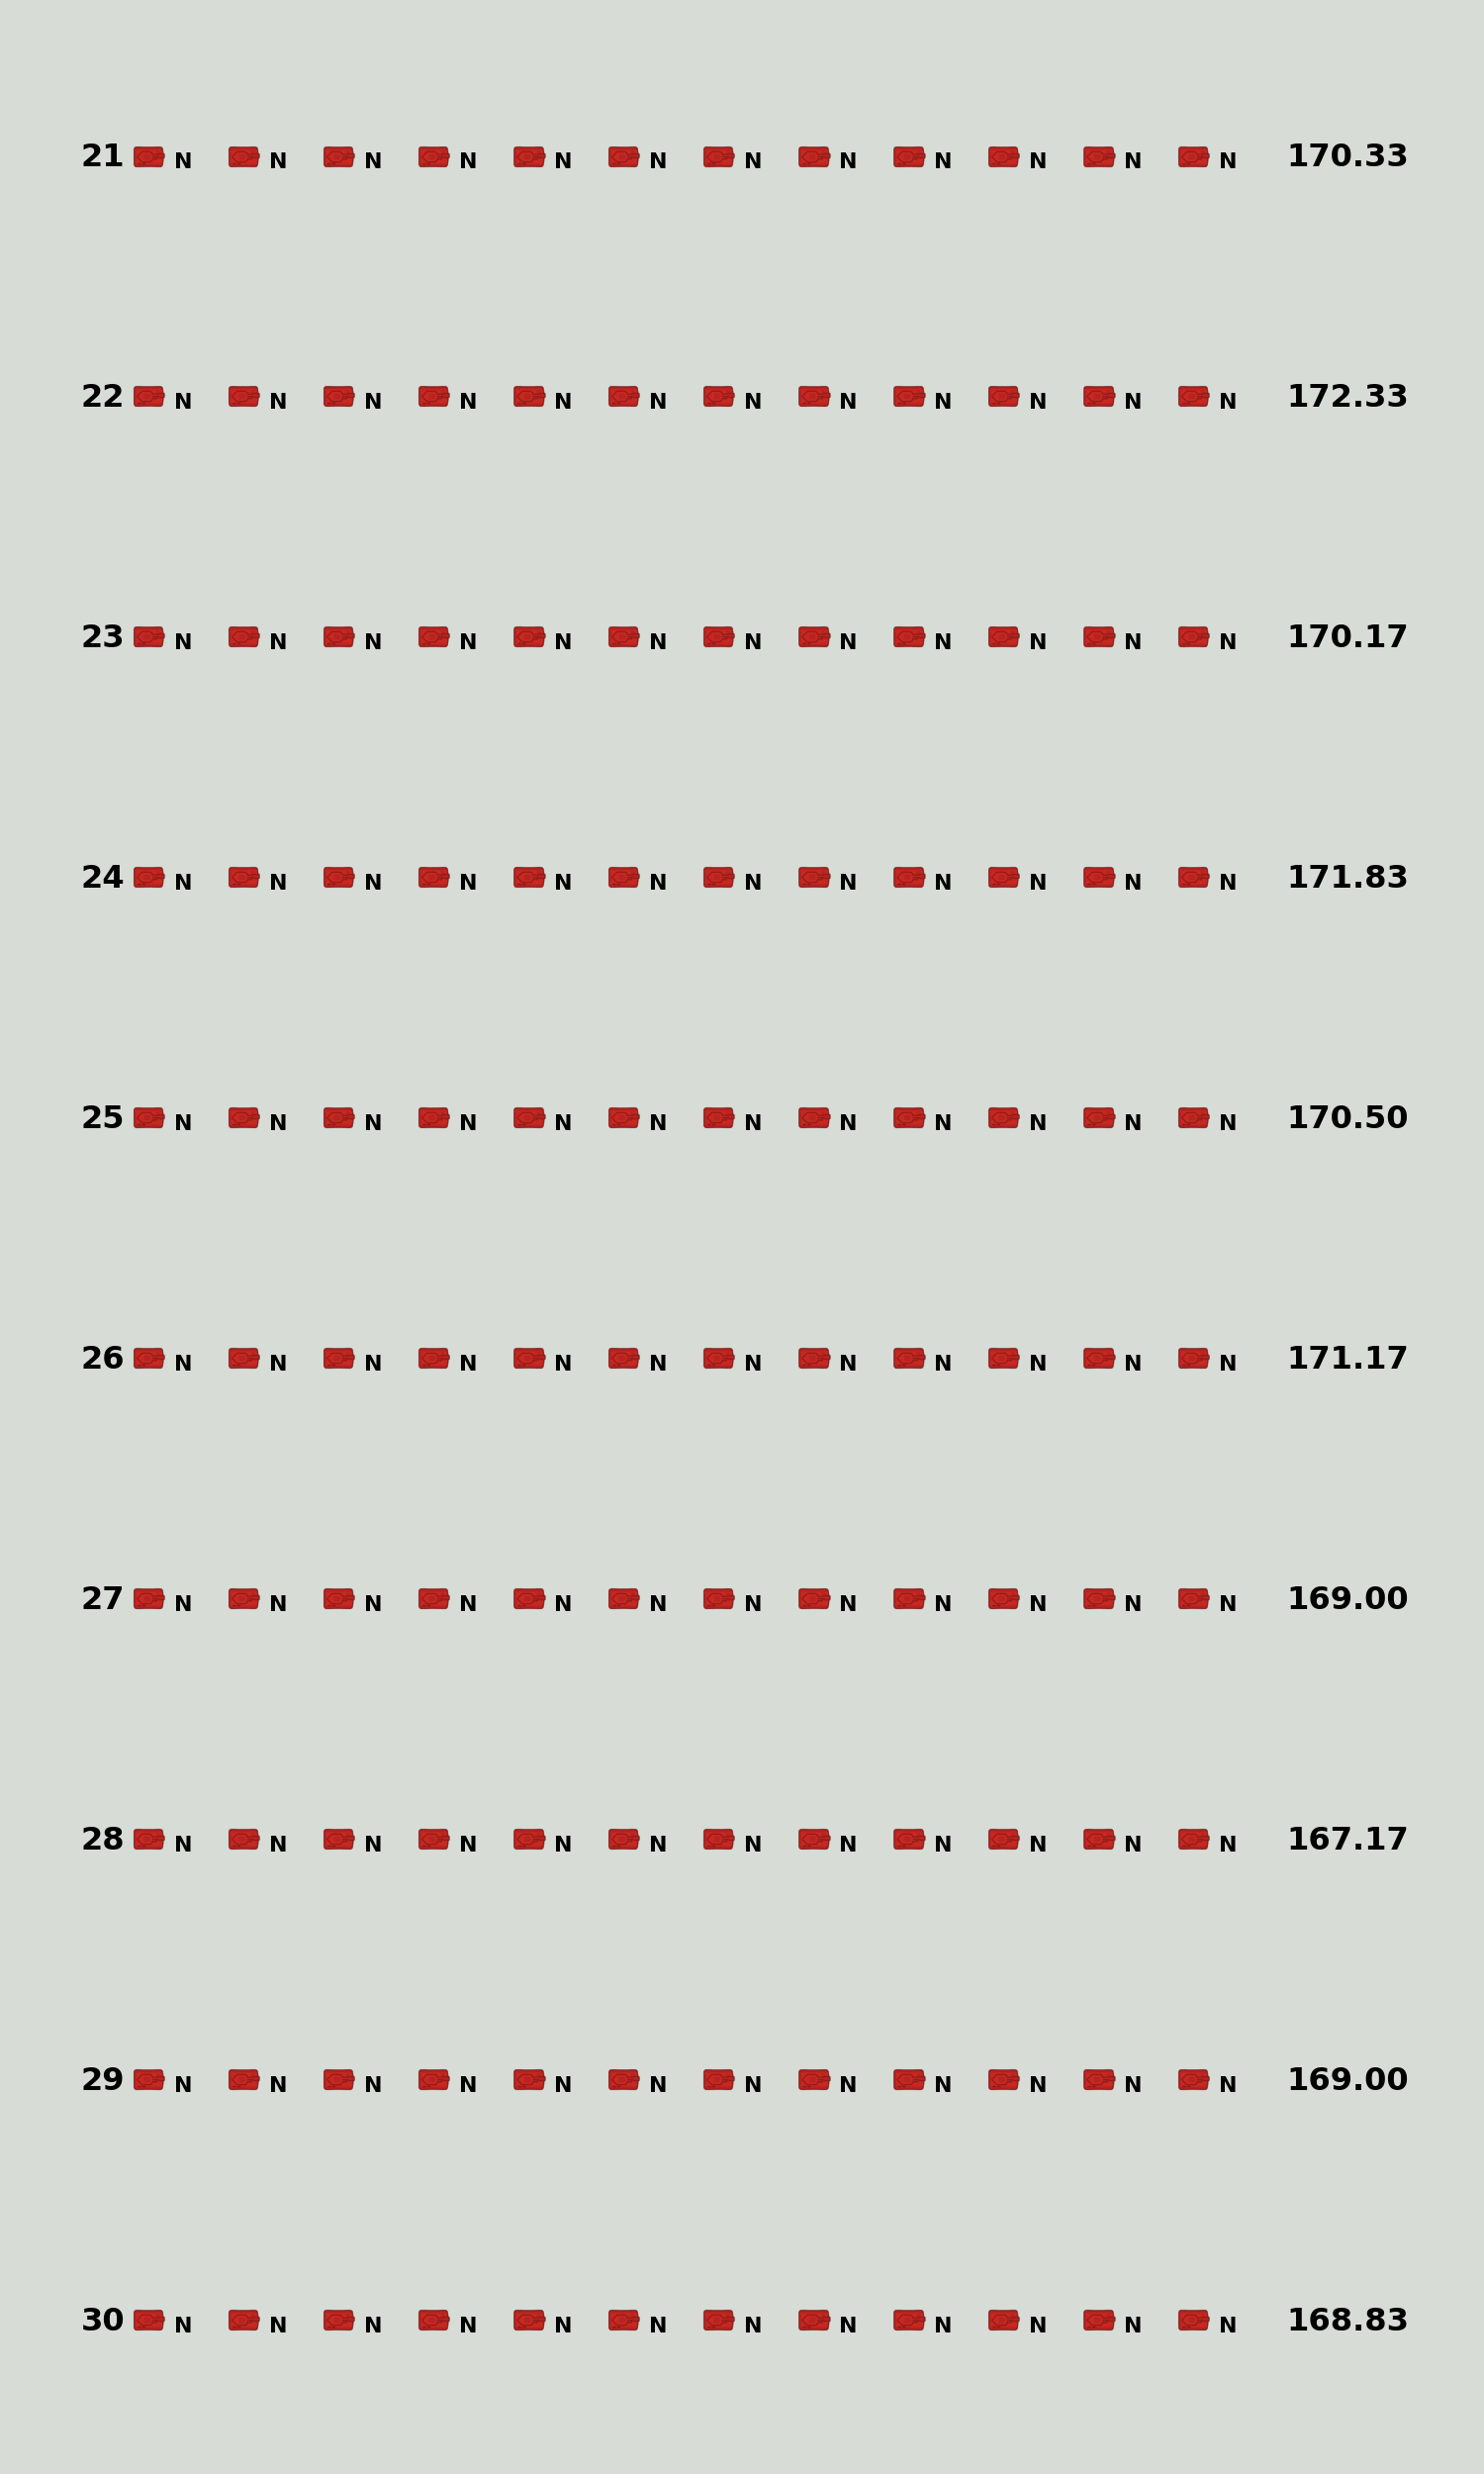
\includegraphics[width=0.9\textwidth]{figuras/td/td_allred_ai_mode_3_3.png}
  \caption{Visualização da moda de cada onda com a versão v3 contra Torres Vermelhas.}
  \label{fig:td-moda-red-3-3}
\end{figure}

%% ------------------------------------------------------------------------- %%
\section{Torres Verde + Vermelha}
\label{sec:apend-moda-td-gr-v3}

\begin{figure}[H]
  \centering
  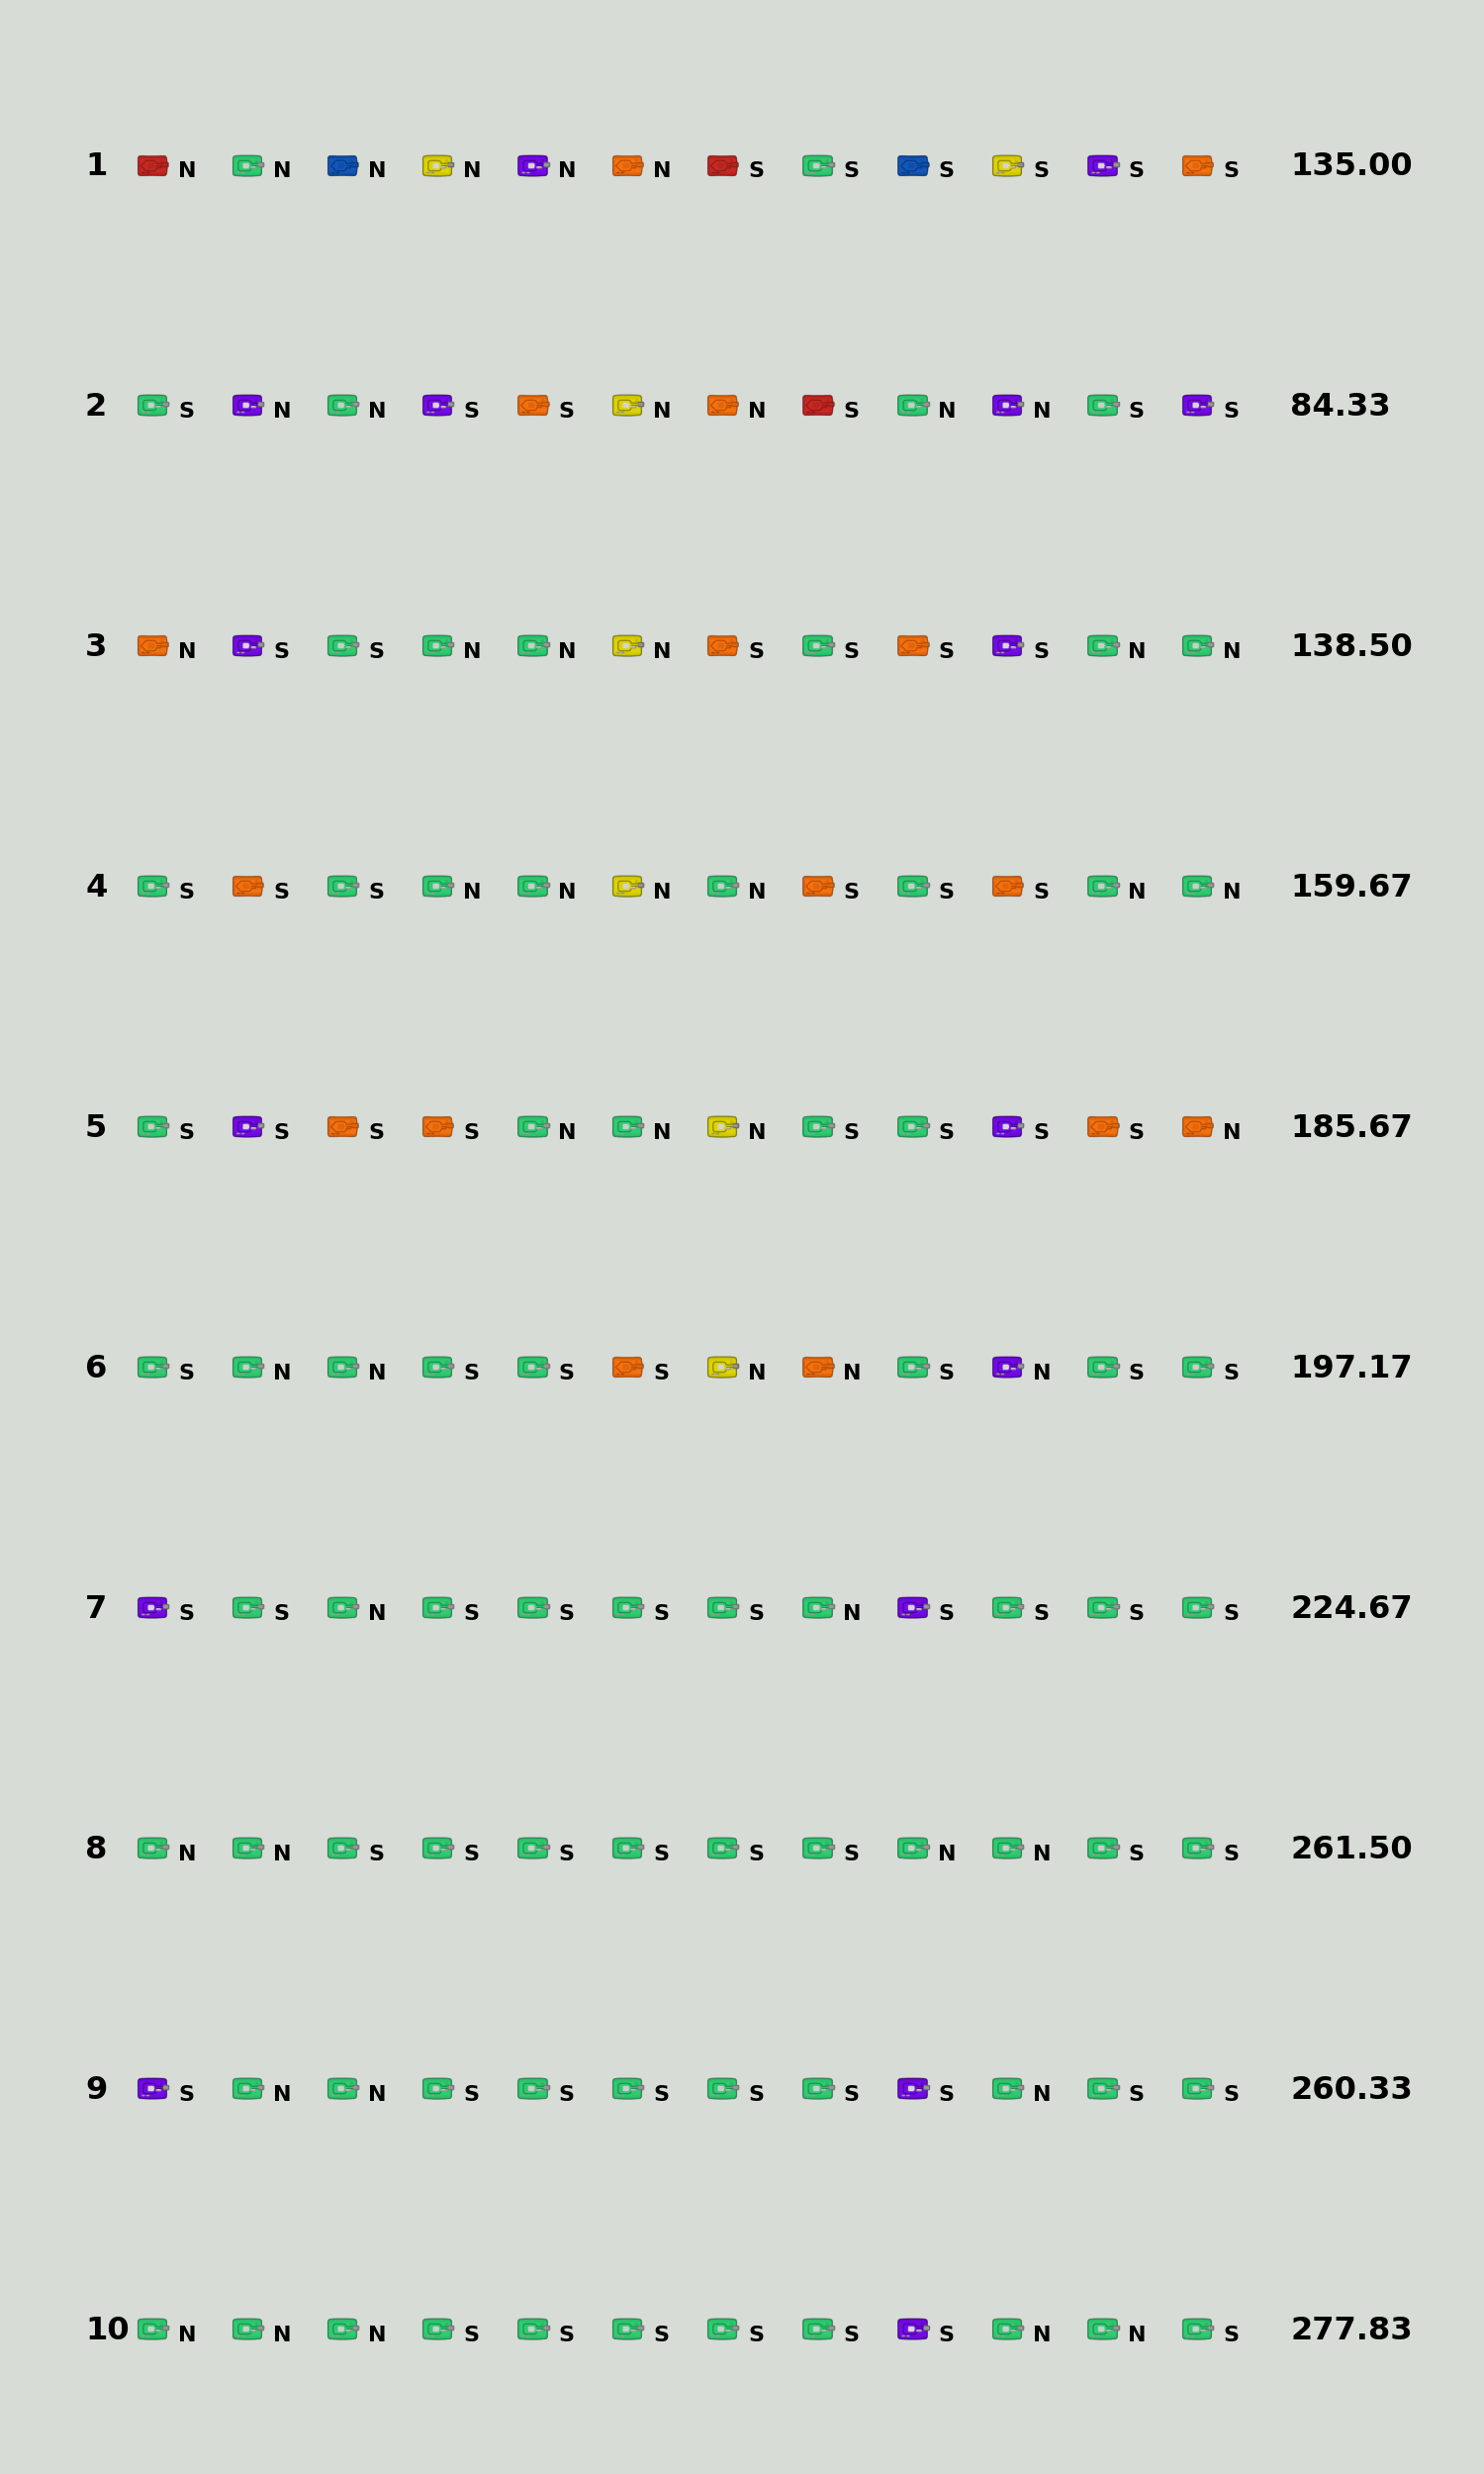
\includegraphics[width=0.9\textwidth]{figuras/td/td_greenred_ai_mode_3_1.png}
  \caption{Visualização da moda de cada onda com a versão v3 contra Torres Verdes + Vermelhas.}
  \label{fig:td-moda-greenred-3-1}
\end{figure}

\begin{figure}[H]
  \centering
  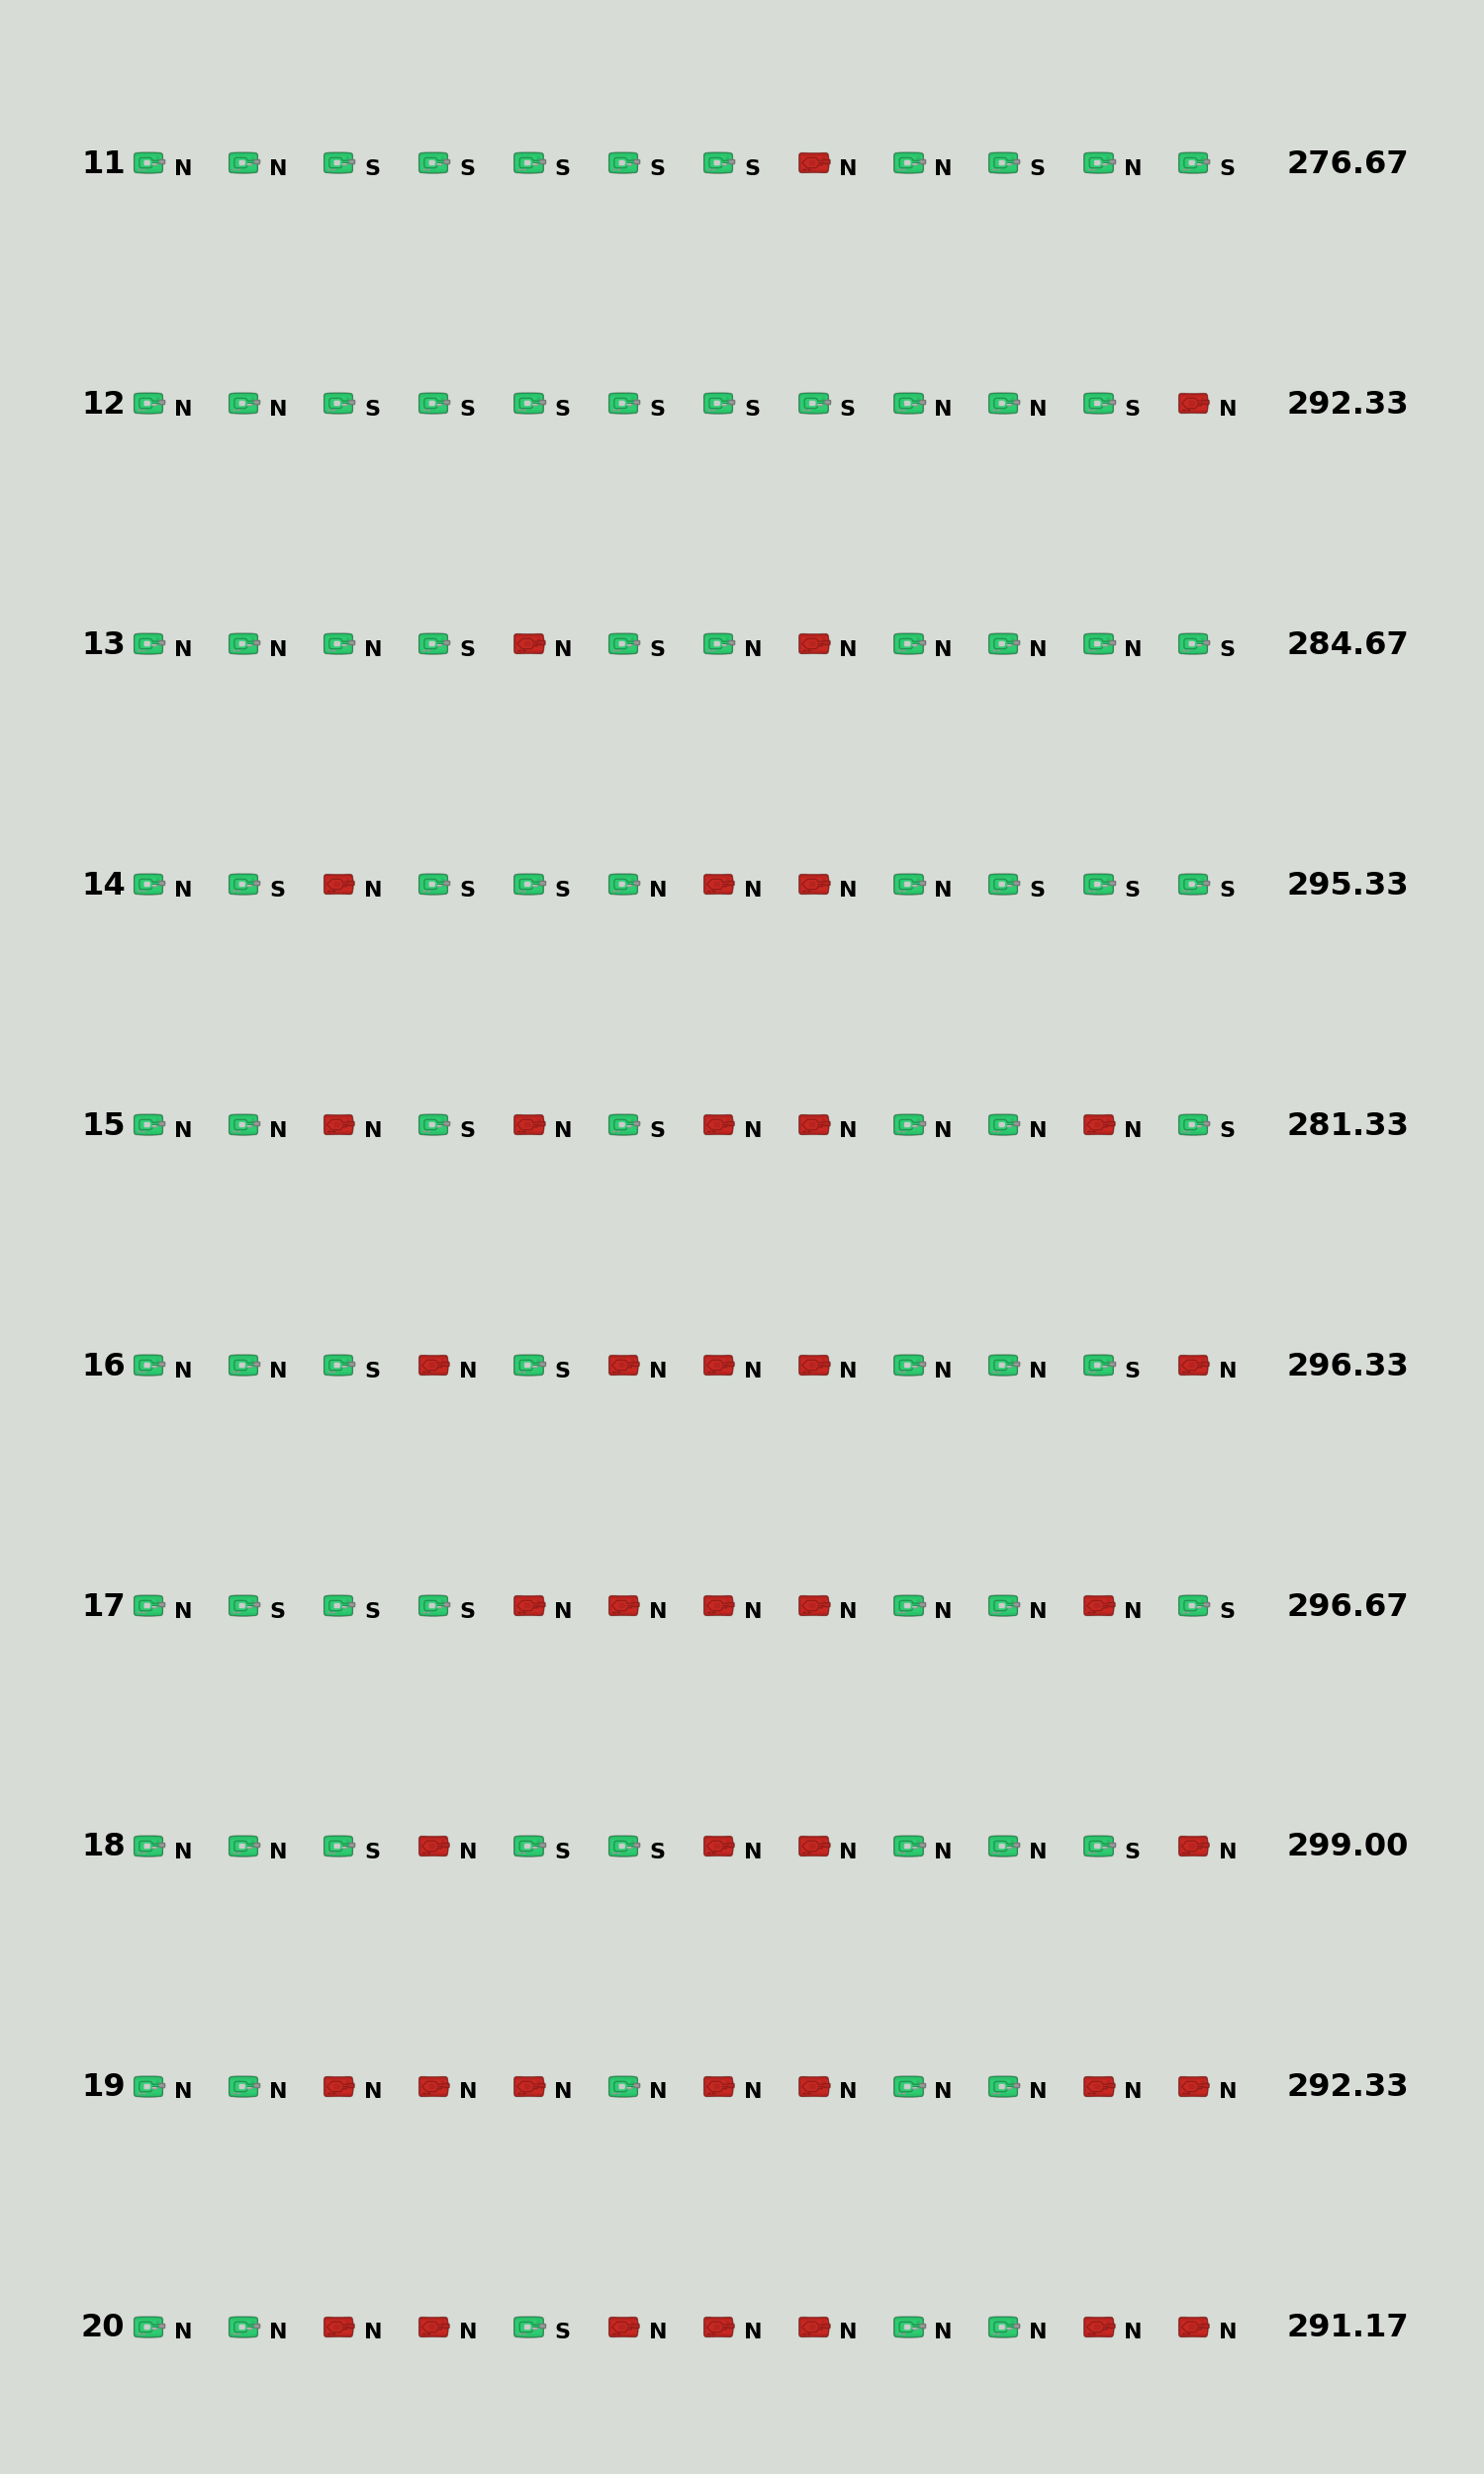
\includegraphics[width=0.9\textwidth]{figuras/td/td_greenred_ai_mode_3_2.png}
  \caption{Visualização da moda de cada onda com a versão v3 contra Torres Verdes + Vermelhas.}
  \label{fig:td-moda-greenred-3-2}
\end{figure}

\begin{figure}[H]
  \centering
  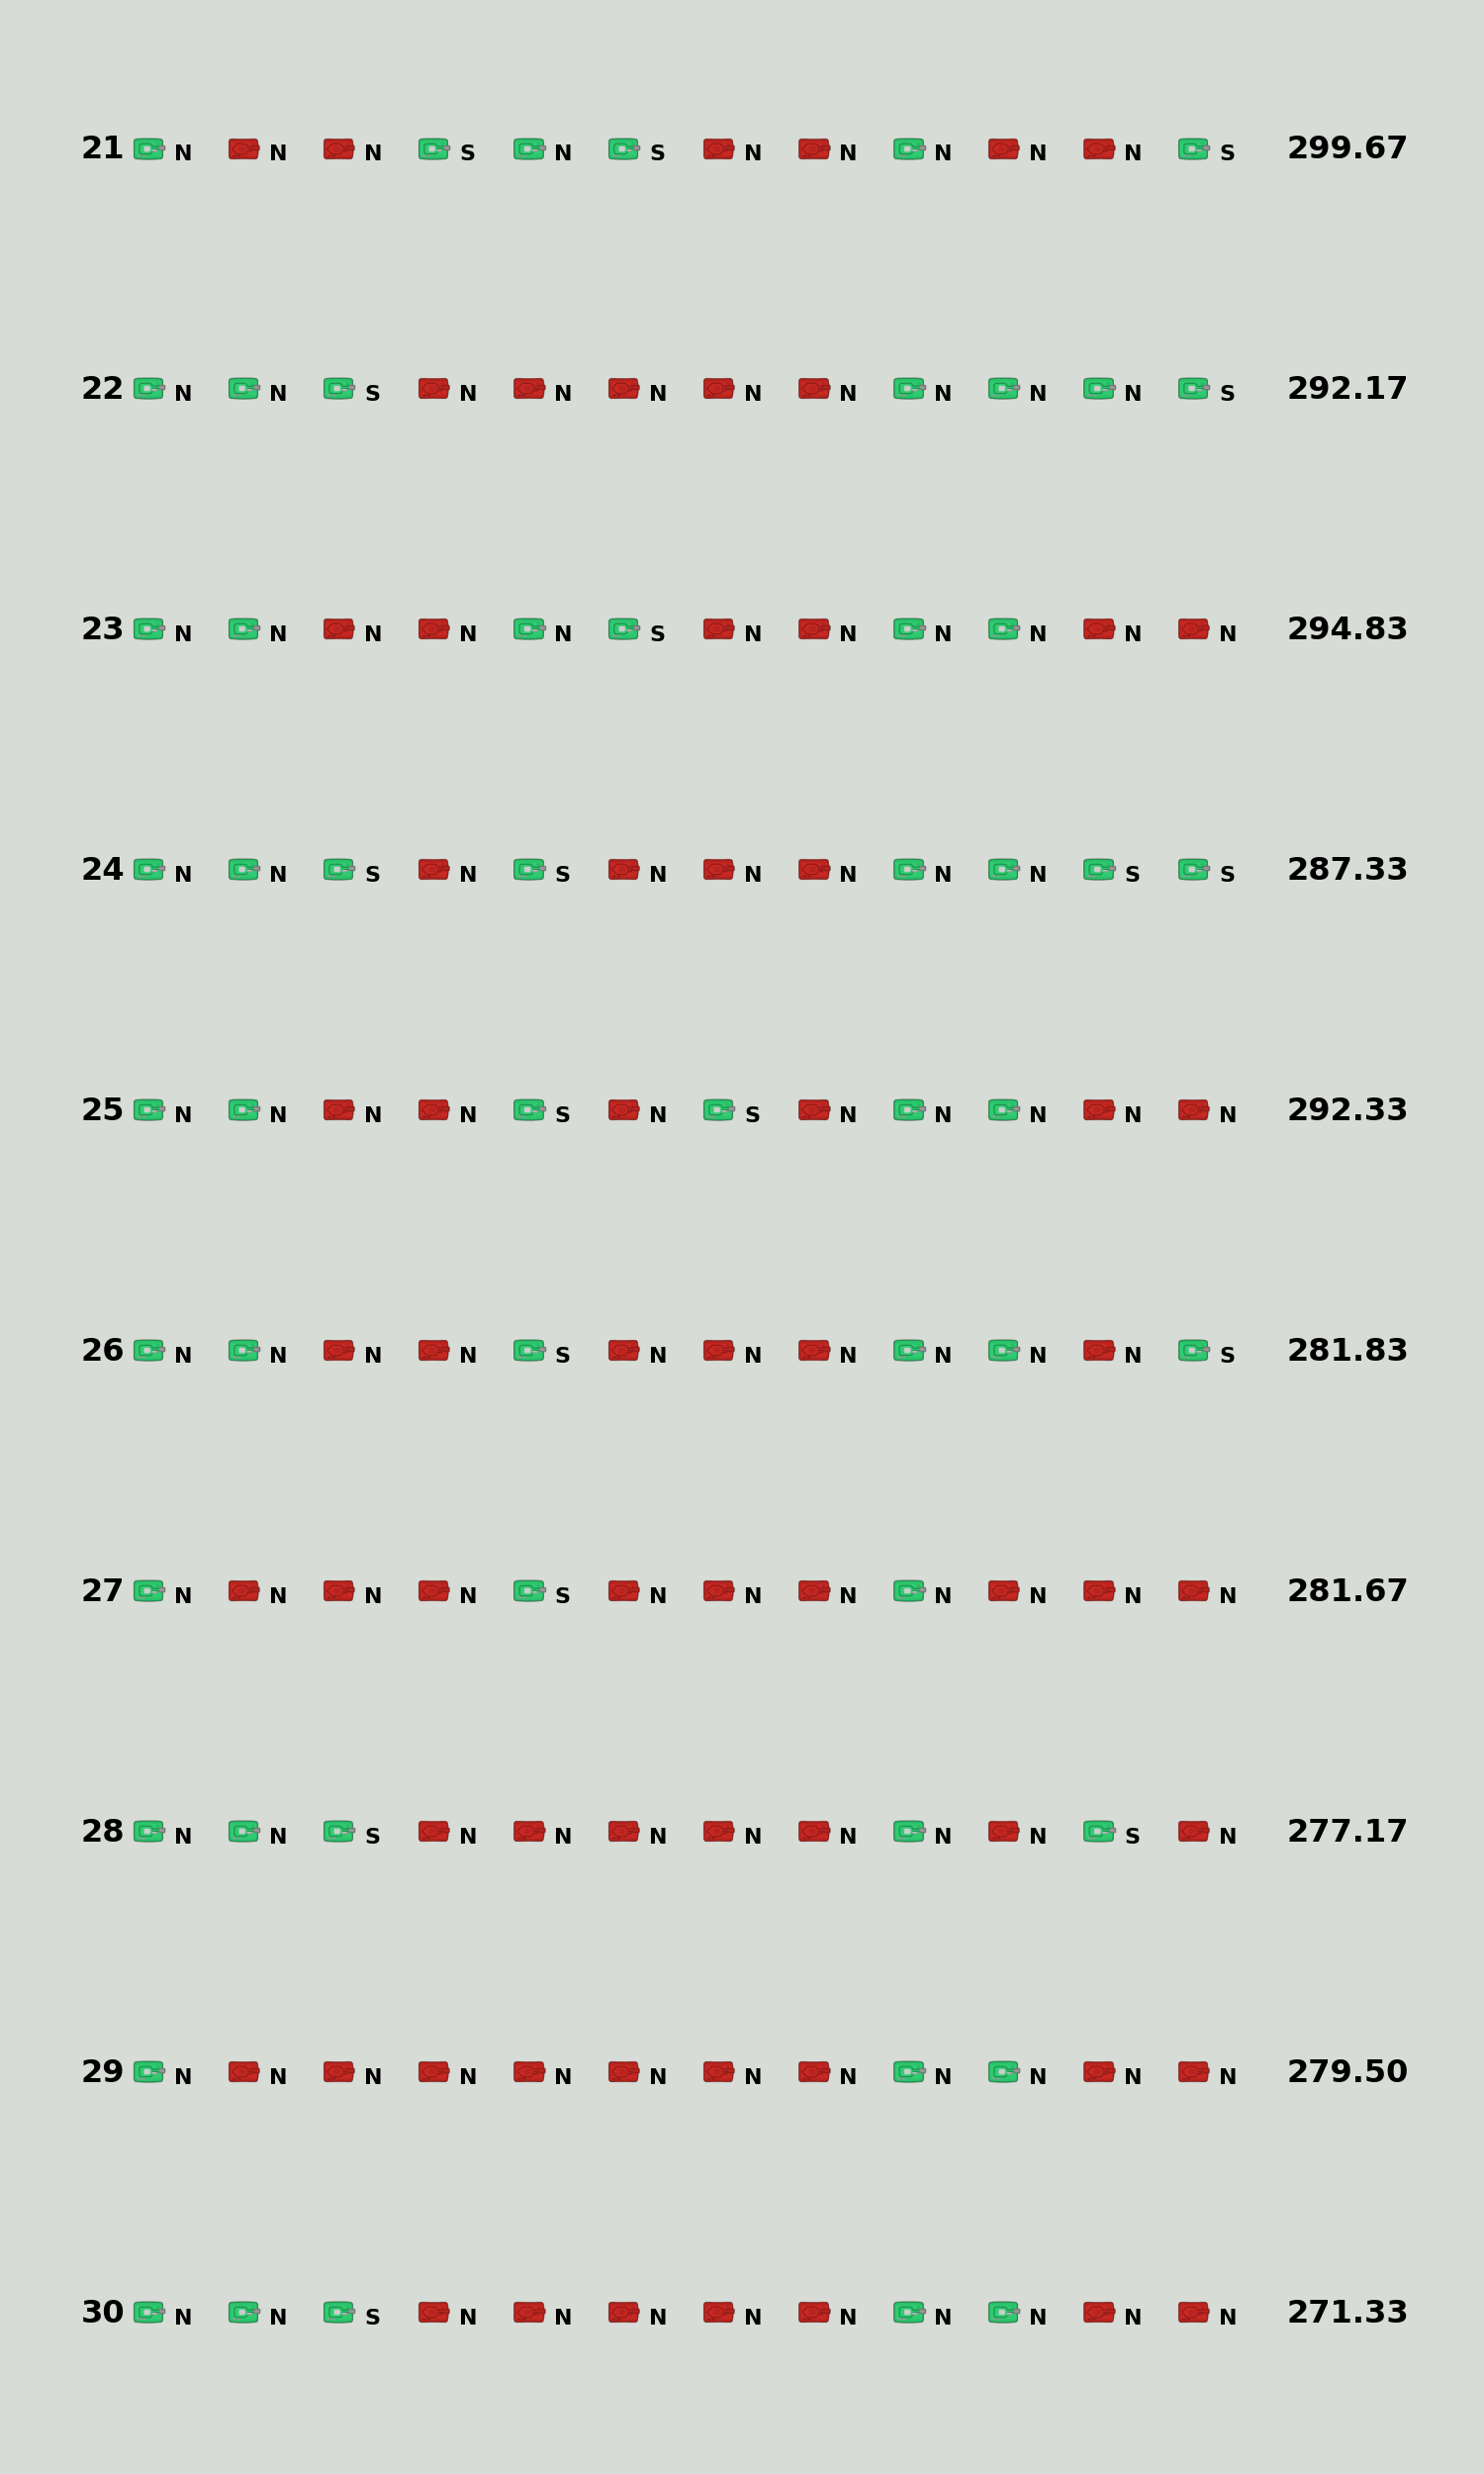
\includegraphics[width=0.9\textwidth]{figuras/td/td_greenred_ai_mode_3_3.png}
  \caption{Visualização da moda de cada onda com a versão v3 contra Torres Verdes + Vermelhas.}
  \label{fig:td-moda-greenred-3-3}
\end{figure}

%% ------------------------------------------------------------------------- %%
\section{Torres Vermelha + Verde}
\label{sec:apend-moda-td-rg-v3}

\begin{figure}[H]
  \centering
  \includegraphics[width=0.9\textwidth]{figuras/td/td_redgreen_ai_mode_3_1.png}
  \caption{Visualização da moda de cada onda com a versão v3 contra Torres Vermelhas + Verdes.}
  \label{fig:td-moda-redgreen-3-1}
\end{figure}

\begin{figure}[H]
  \centering
  \includegraphics[width=0.9\textwidth]{figuras/td/td_redgreen_ai_mode_3_2.png}
  \caption{Visualização da moda de cada onda com a versão v3 contra Torres Vermelhas + Verdes.}
  \label{fig:td-moda-redgreen-3-2}
\end{figure}

\begin{figure}[H]
  \centering
  \includegraphics[width=0.9\textwidth]{figuras/td/td_redgreen_ai_mode_3_3.png}
  \caption{Visualização da moda de cada onda com a versão v3 contra Torres Vermelhas + Verdes.}
  \label{fig:td-moda-redgreen-3-3}
\end{figure}
\par

%% ------------------------------------------------------------------------- %%
\chapter{Moda das Ondas no Space Shooter para versão v1}
\label{sec:apend-moda-ss-v1}

Foram calculadas as modas das ondas do \textit{fitness} desenvolvido, para permitir a visualização dos inimigos mais comuns que o algoritmo convergiu.

%% ------------------------------------------------------------------------- %%
\section{Nave Parada com Disparo Amarelo}
\label{sec:apend-moda-ss-ys-v1}

\begin{figure}[H]
  \centering
  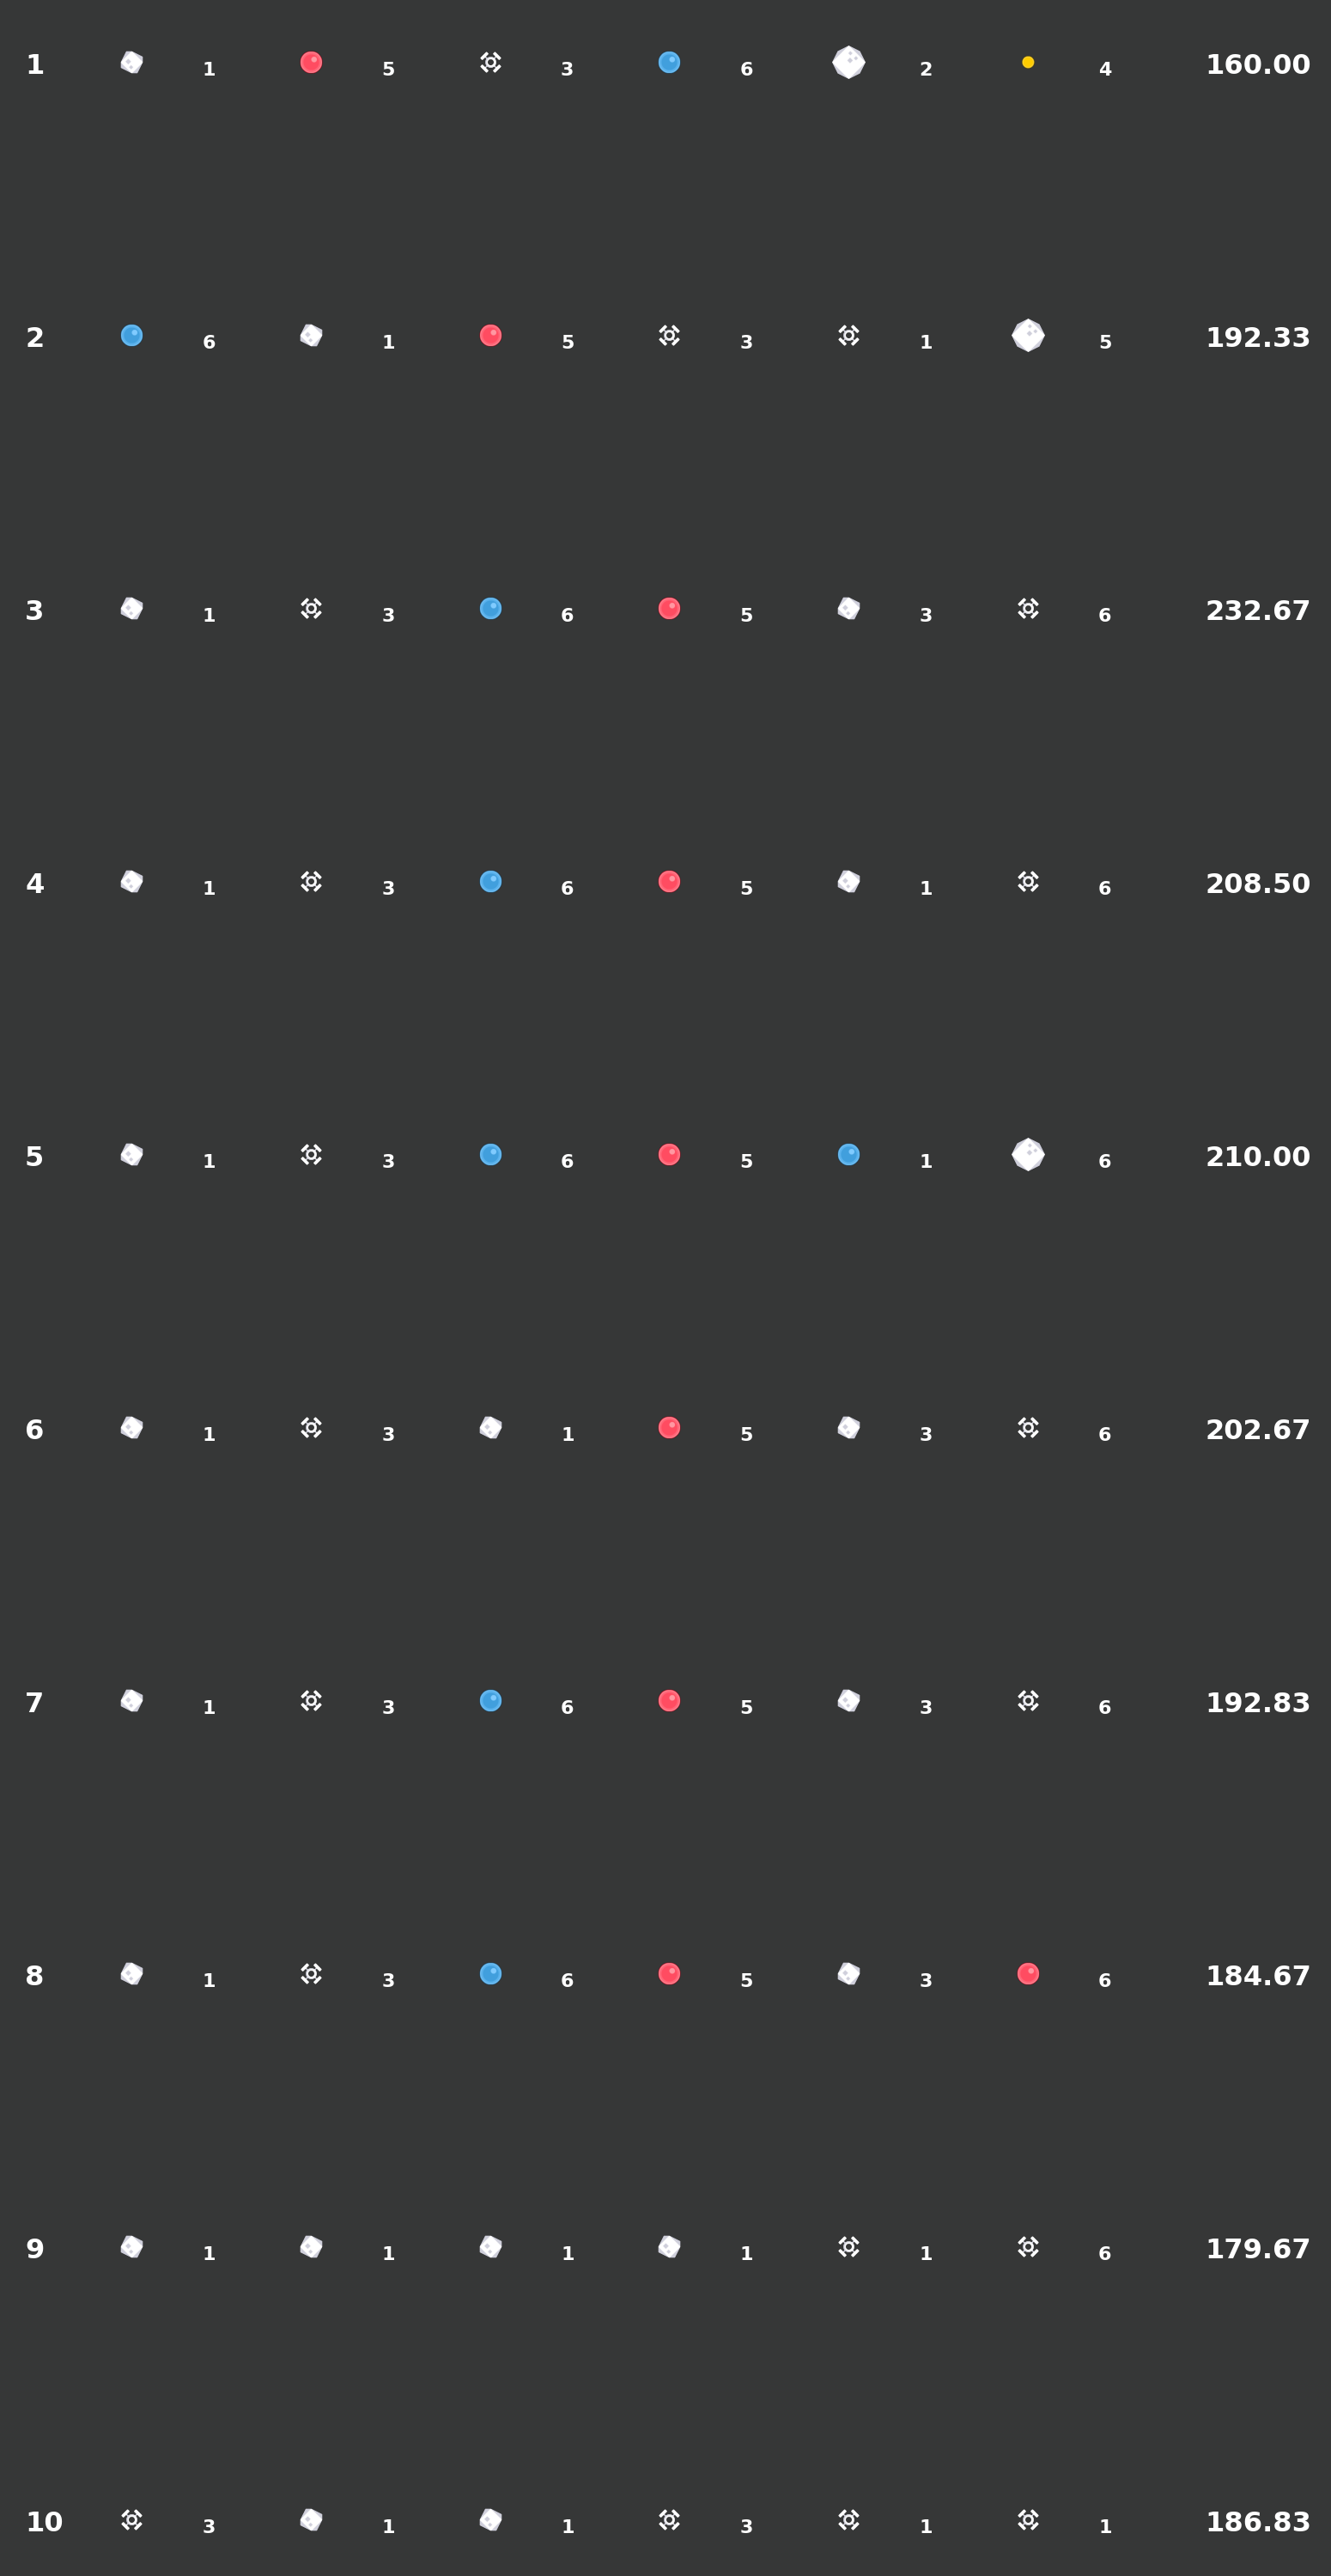
\includegraphics[width=0.7\textwidth]{figuras/ss/ss_yellowstill_ai_mode_1_1.png}
  \caption{Visualização da moda de cada onda com a versão v1 contra Nave Parada, Disparo Amarelo.}
  \label{fig:ss-moda-ys-1-1}
\end{figure}

\begin{figure}[H]
  \centering
  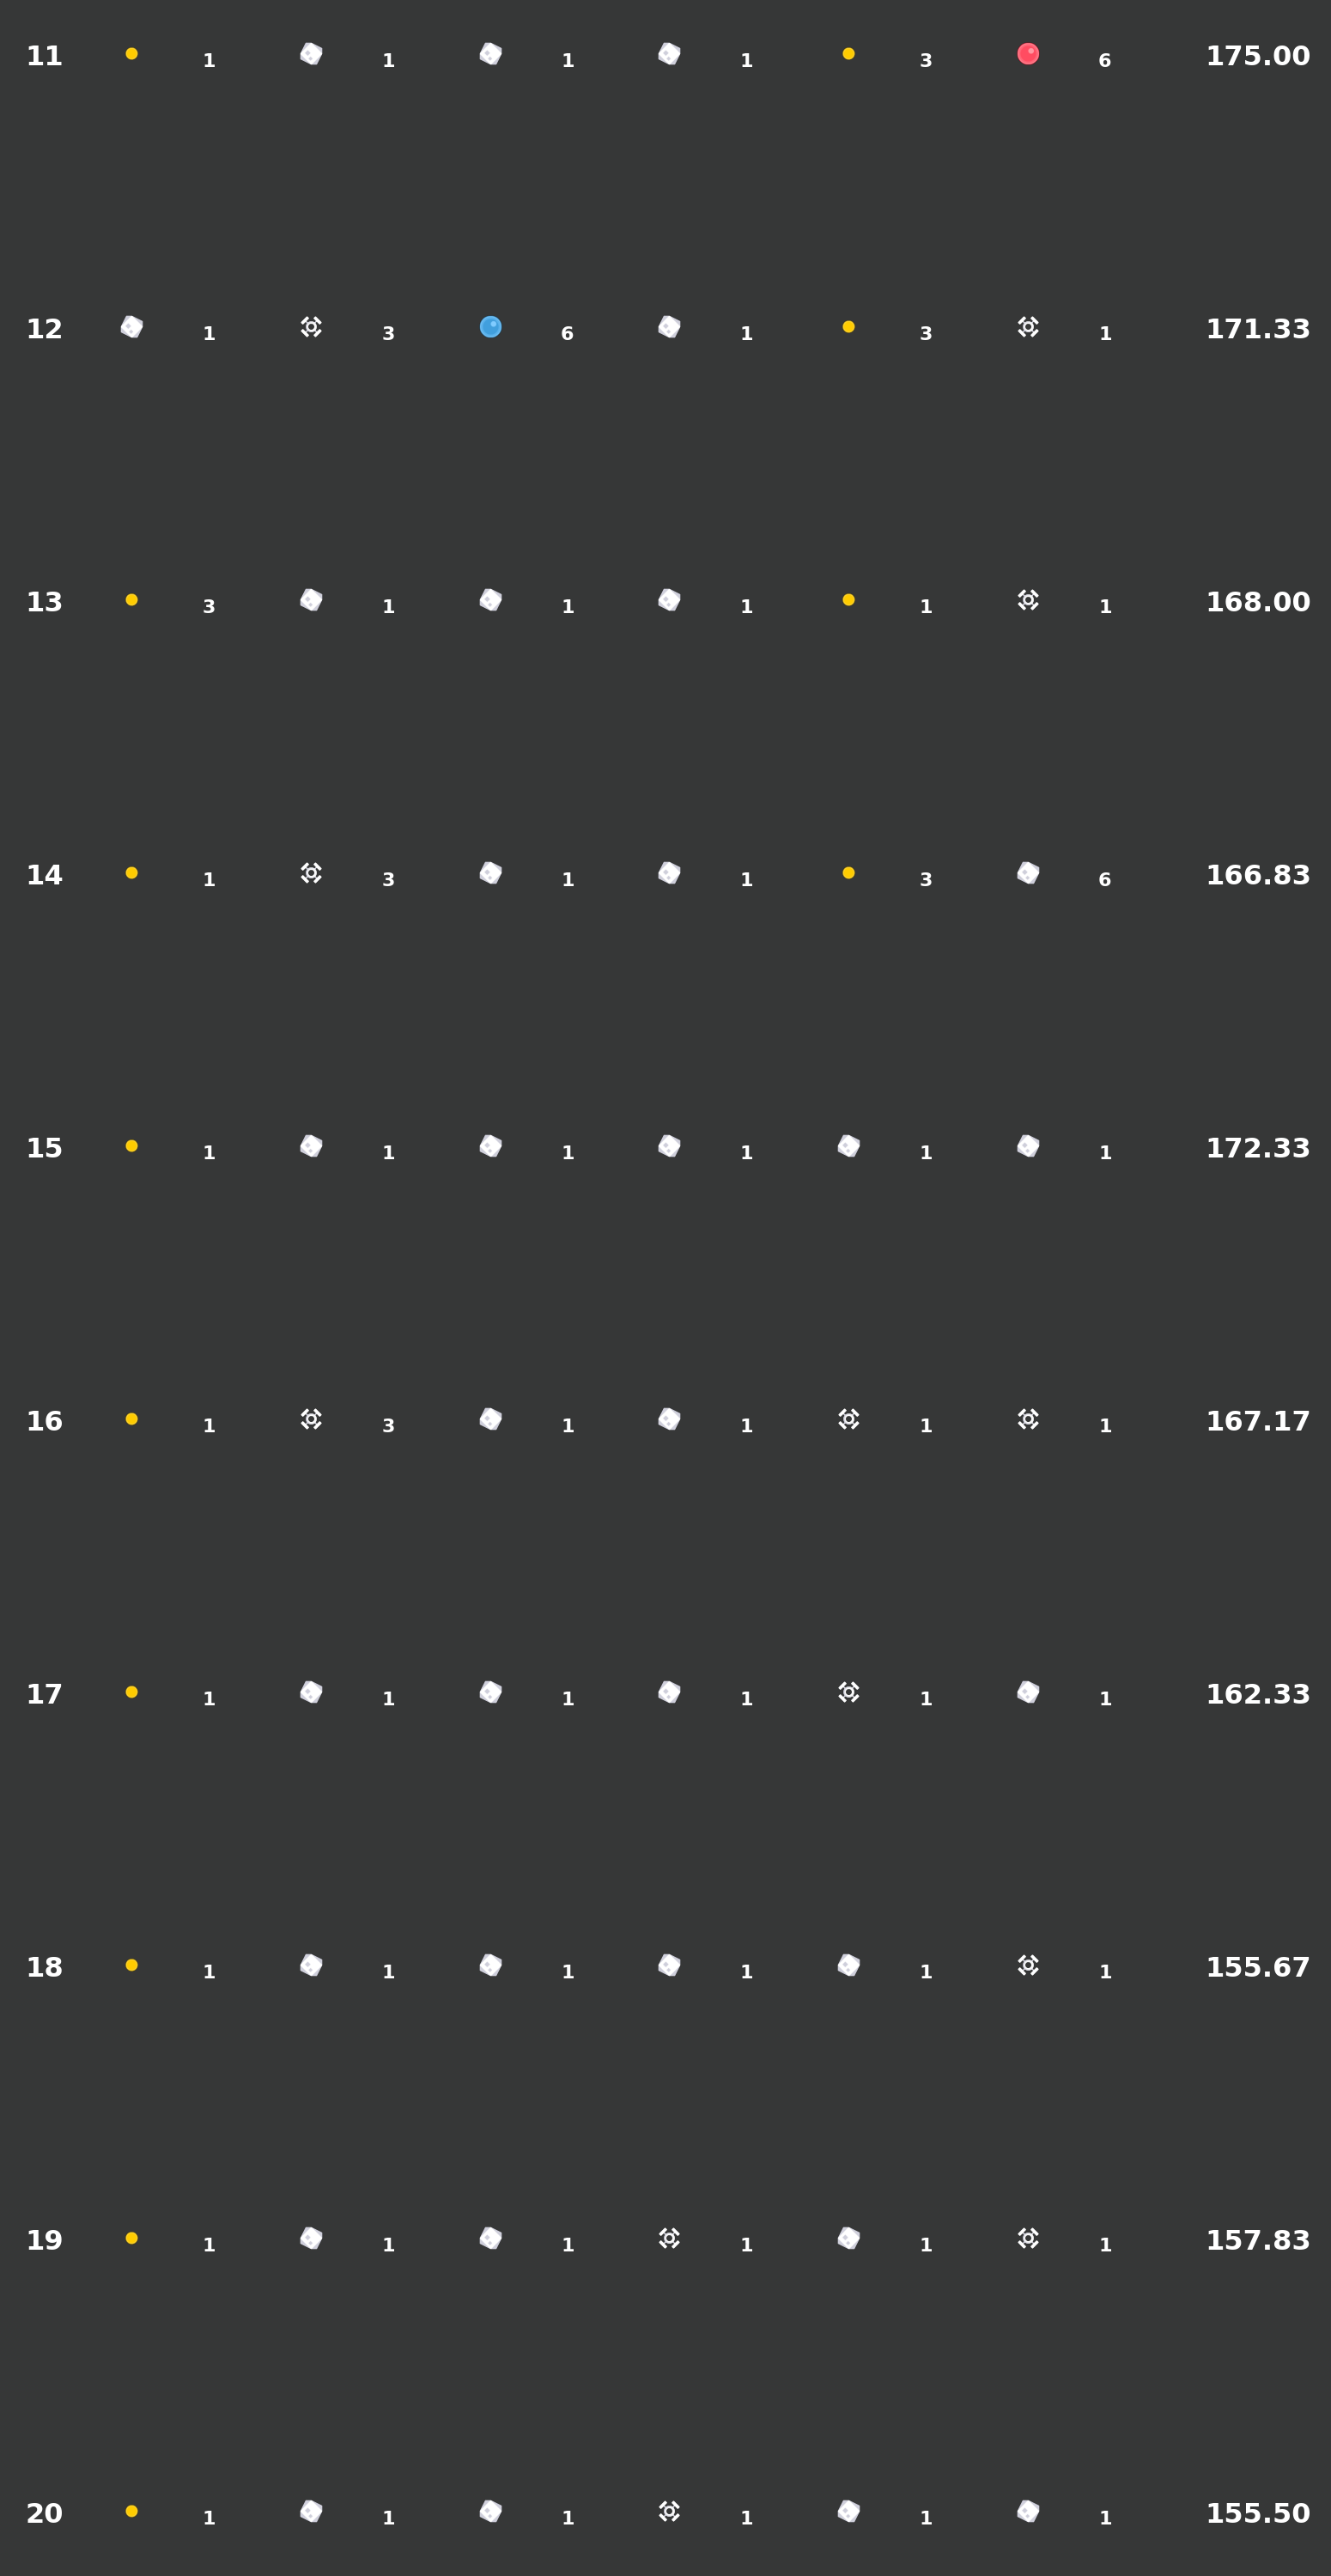
\includegraphics[width=0.7\textwidth]{figuras/ss/ss_yellowstill_ai_mode_1_2.png}
  \caption{Visualização da moda de cada onda com a versão v1 contra Nave Parada, Disparo Amarelo.}
  \label{fig:ss-moda-ys-1-2}
\end{figure}

\begin{figure}[H]
  \centering
  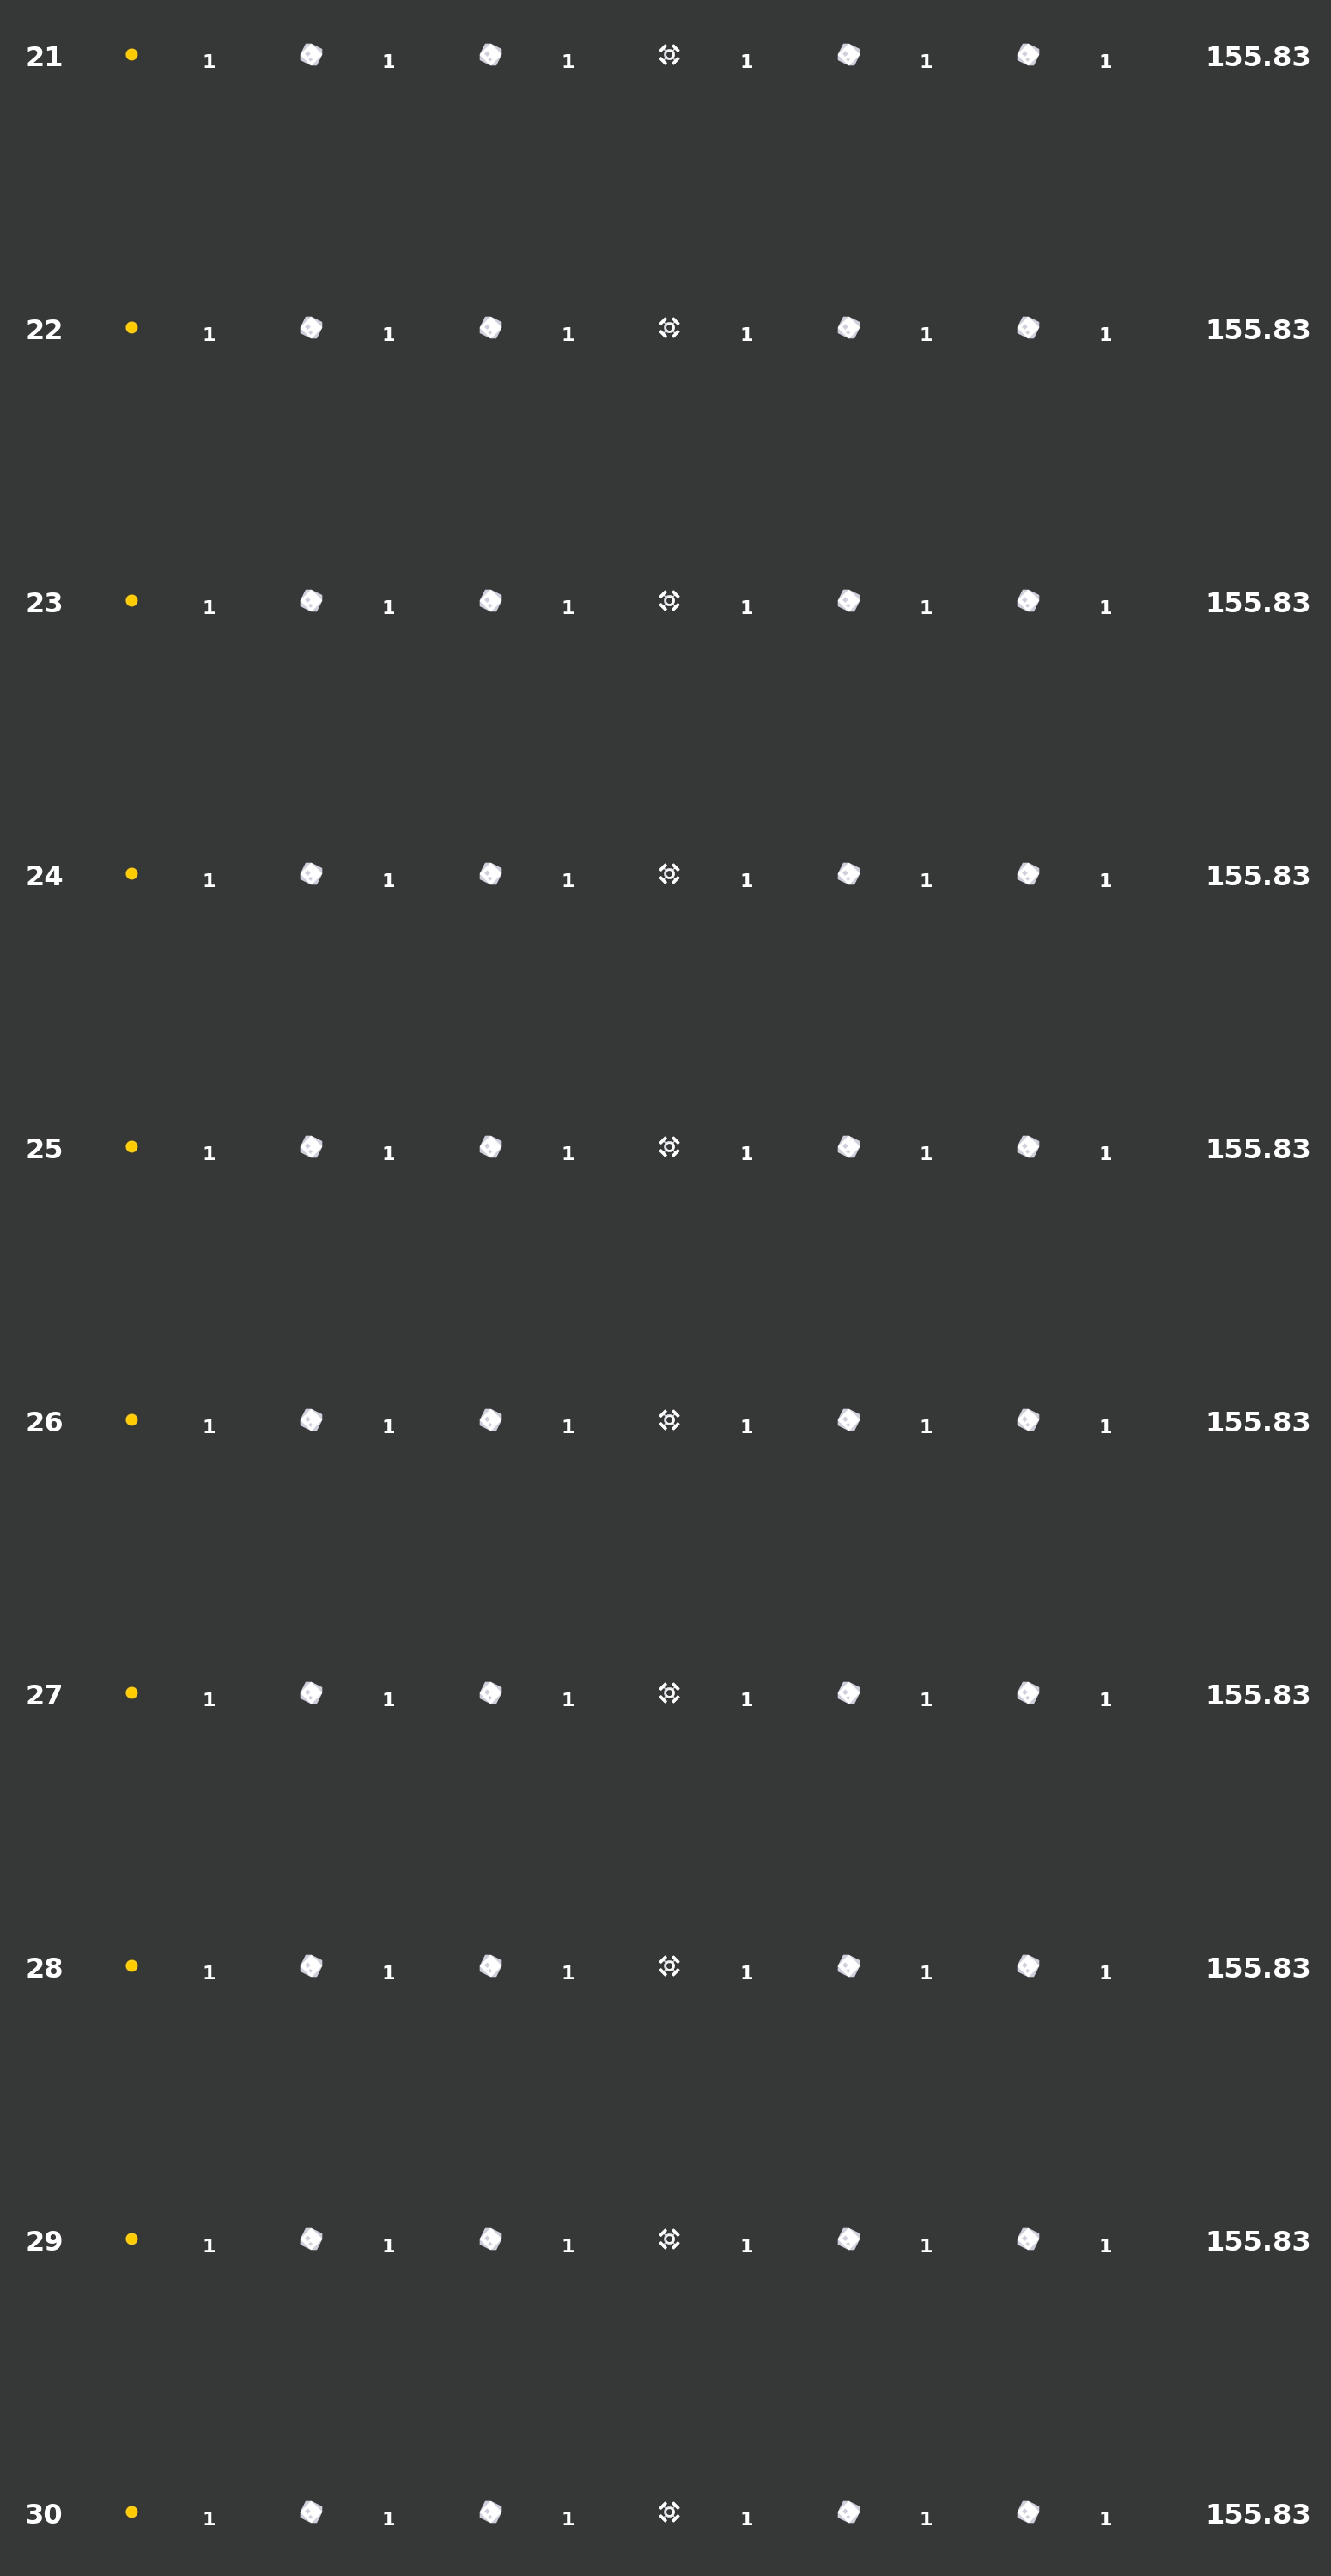
\includegraphics[width=0.7\textwidth]{figuras/ss/ss_yellowstill_ai_mode_1_3.png}
  \caption{Visualização da moda de cada onda com a versão v1 contra Nave Parada, Disparo Amarelo.}
  \label{fig:ss-moda-ys-1-3}
\end{figure}

%% ------------------------------------------------------------------------- %%
\section{Nave Movendo com Disparo Amarelo}
\label{sec:apend-moda-ss-ym-v1}

\begin{figure}[H]
  \centering
  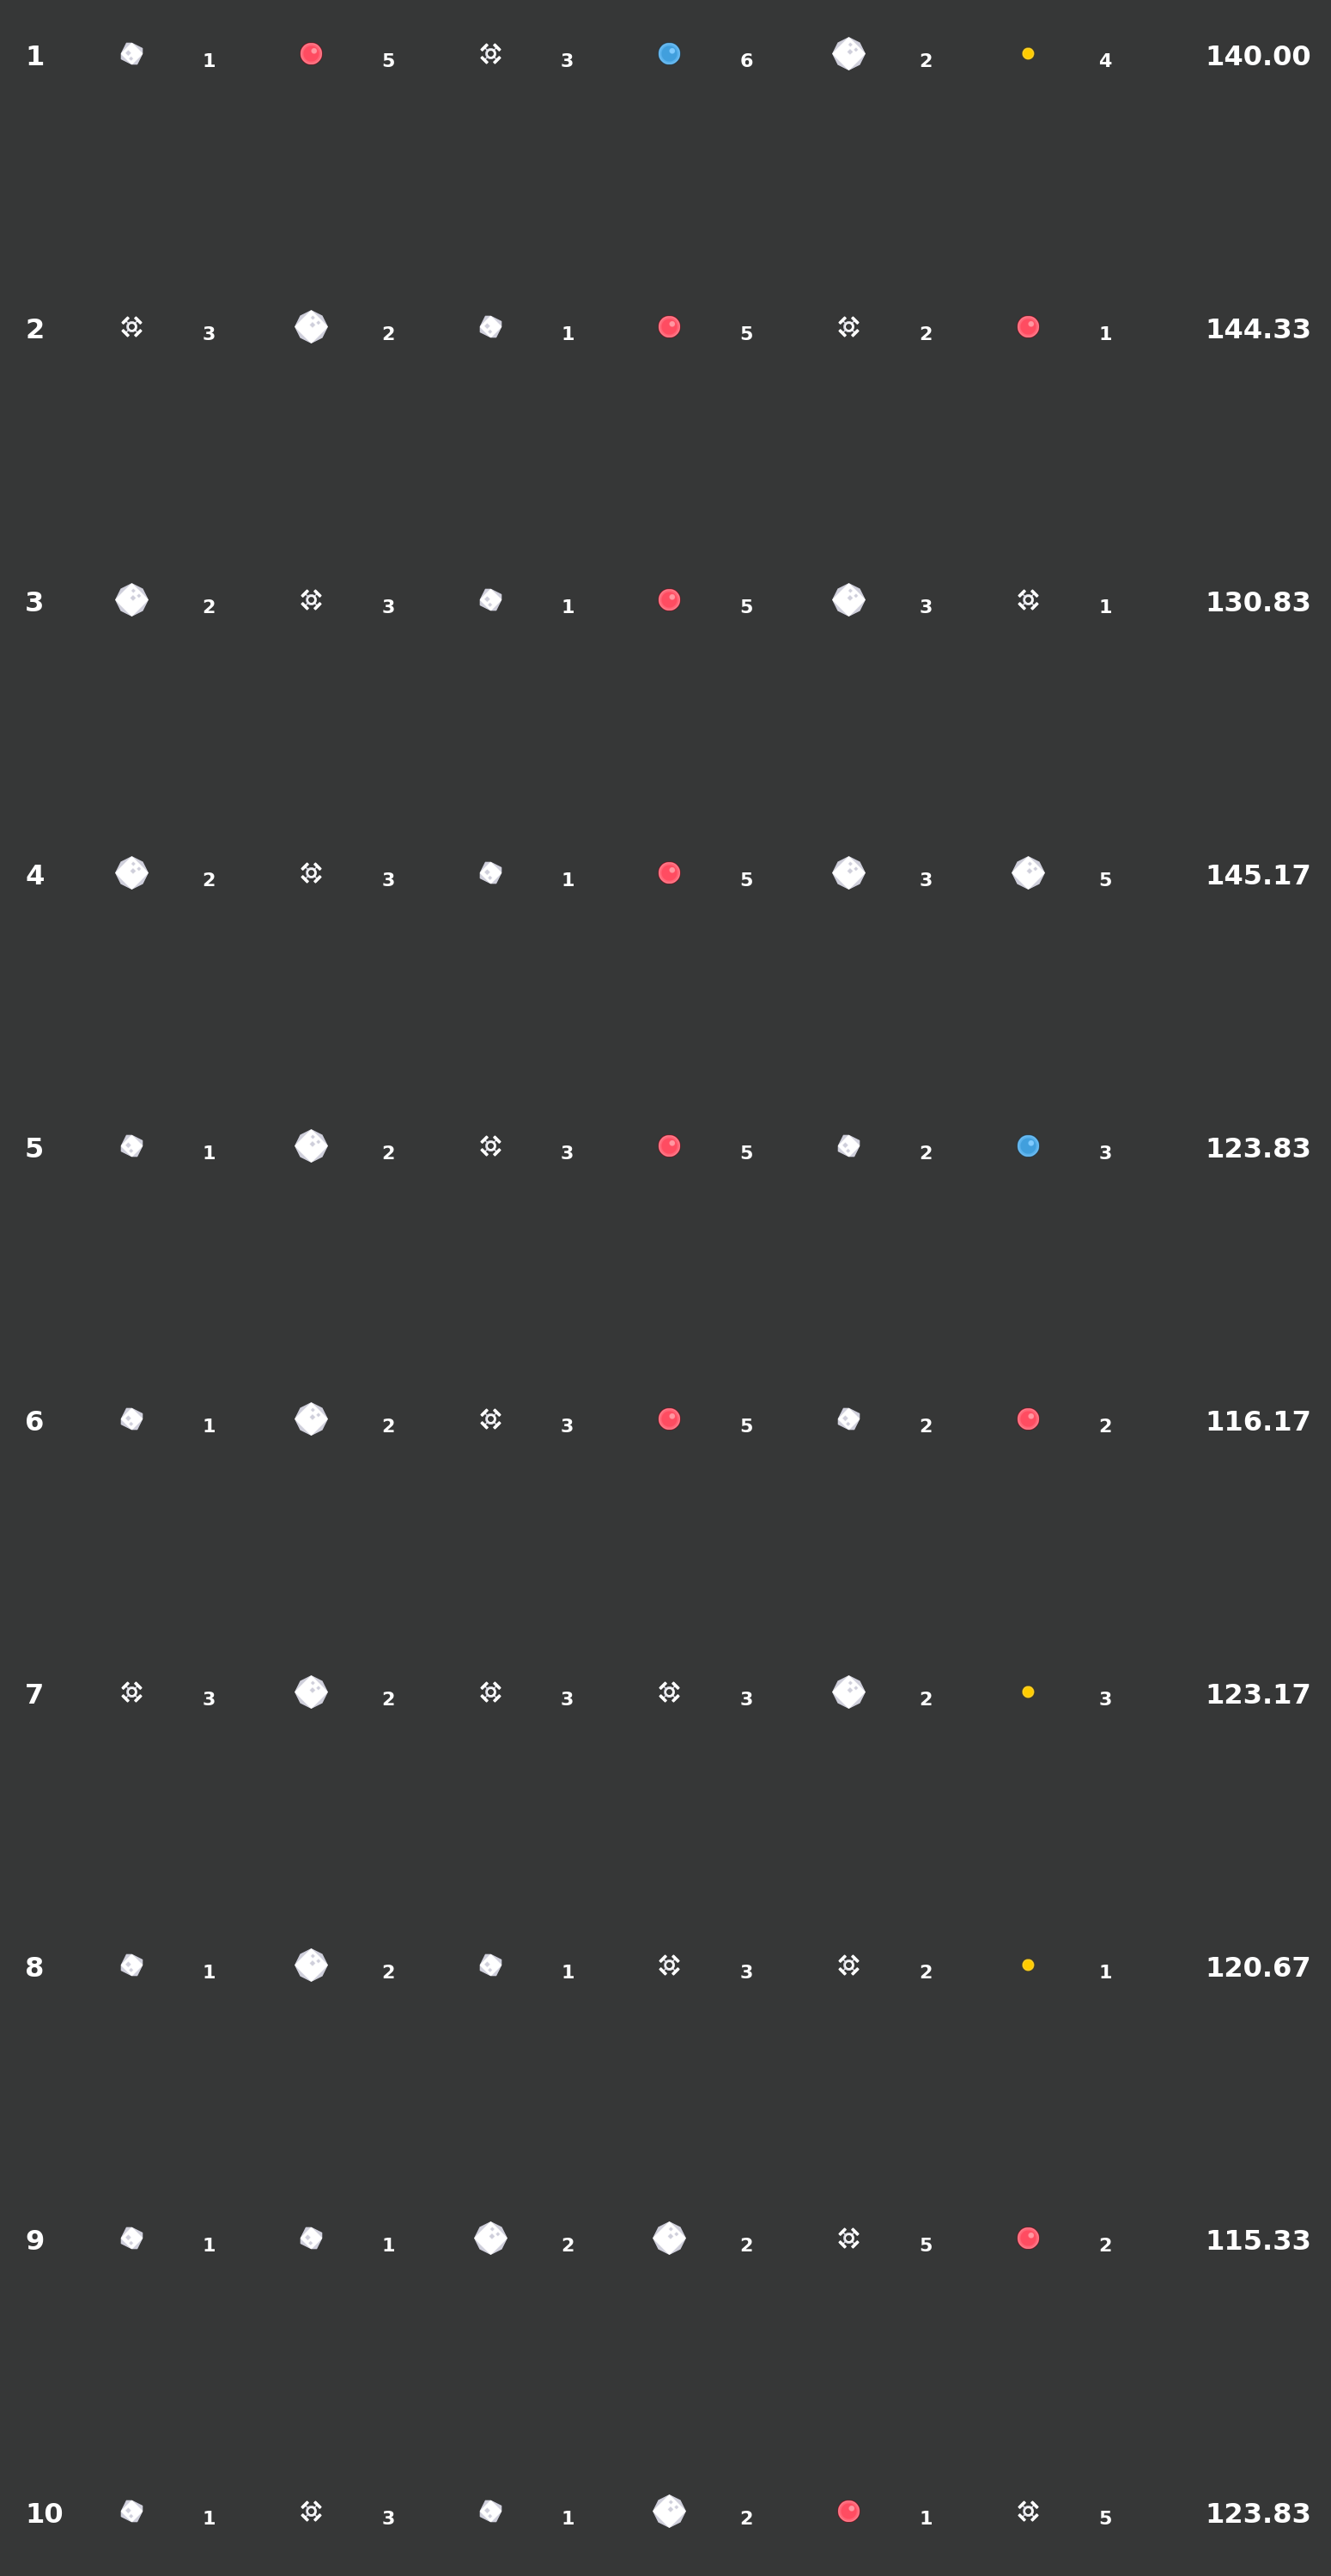
\includegraphics[width=0.7\textwidth]{figuras/ss/ss_yellowmove_ai_mode_1_1.png}
  \caption{Visualização da moda de cada onda com a versão v1 contra Nave Movendo, Disparo Amarelo.}
  \label{fig:ss-moda-ym-1-1}
\end{figure}

\begin{figure}[H]
  \centering
  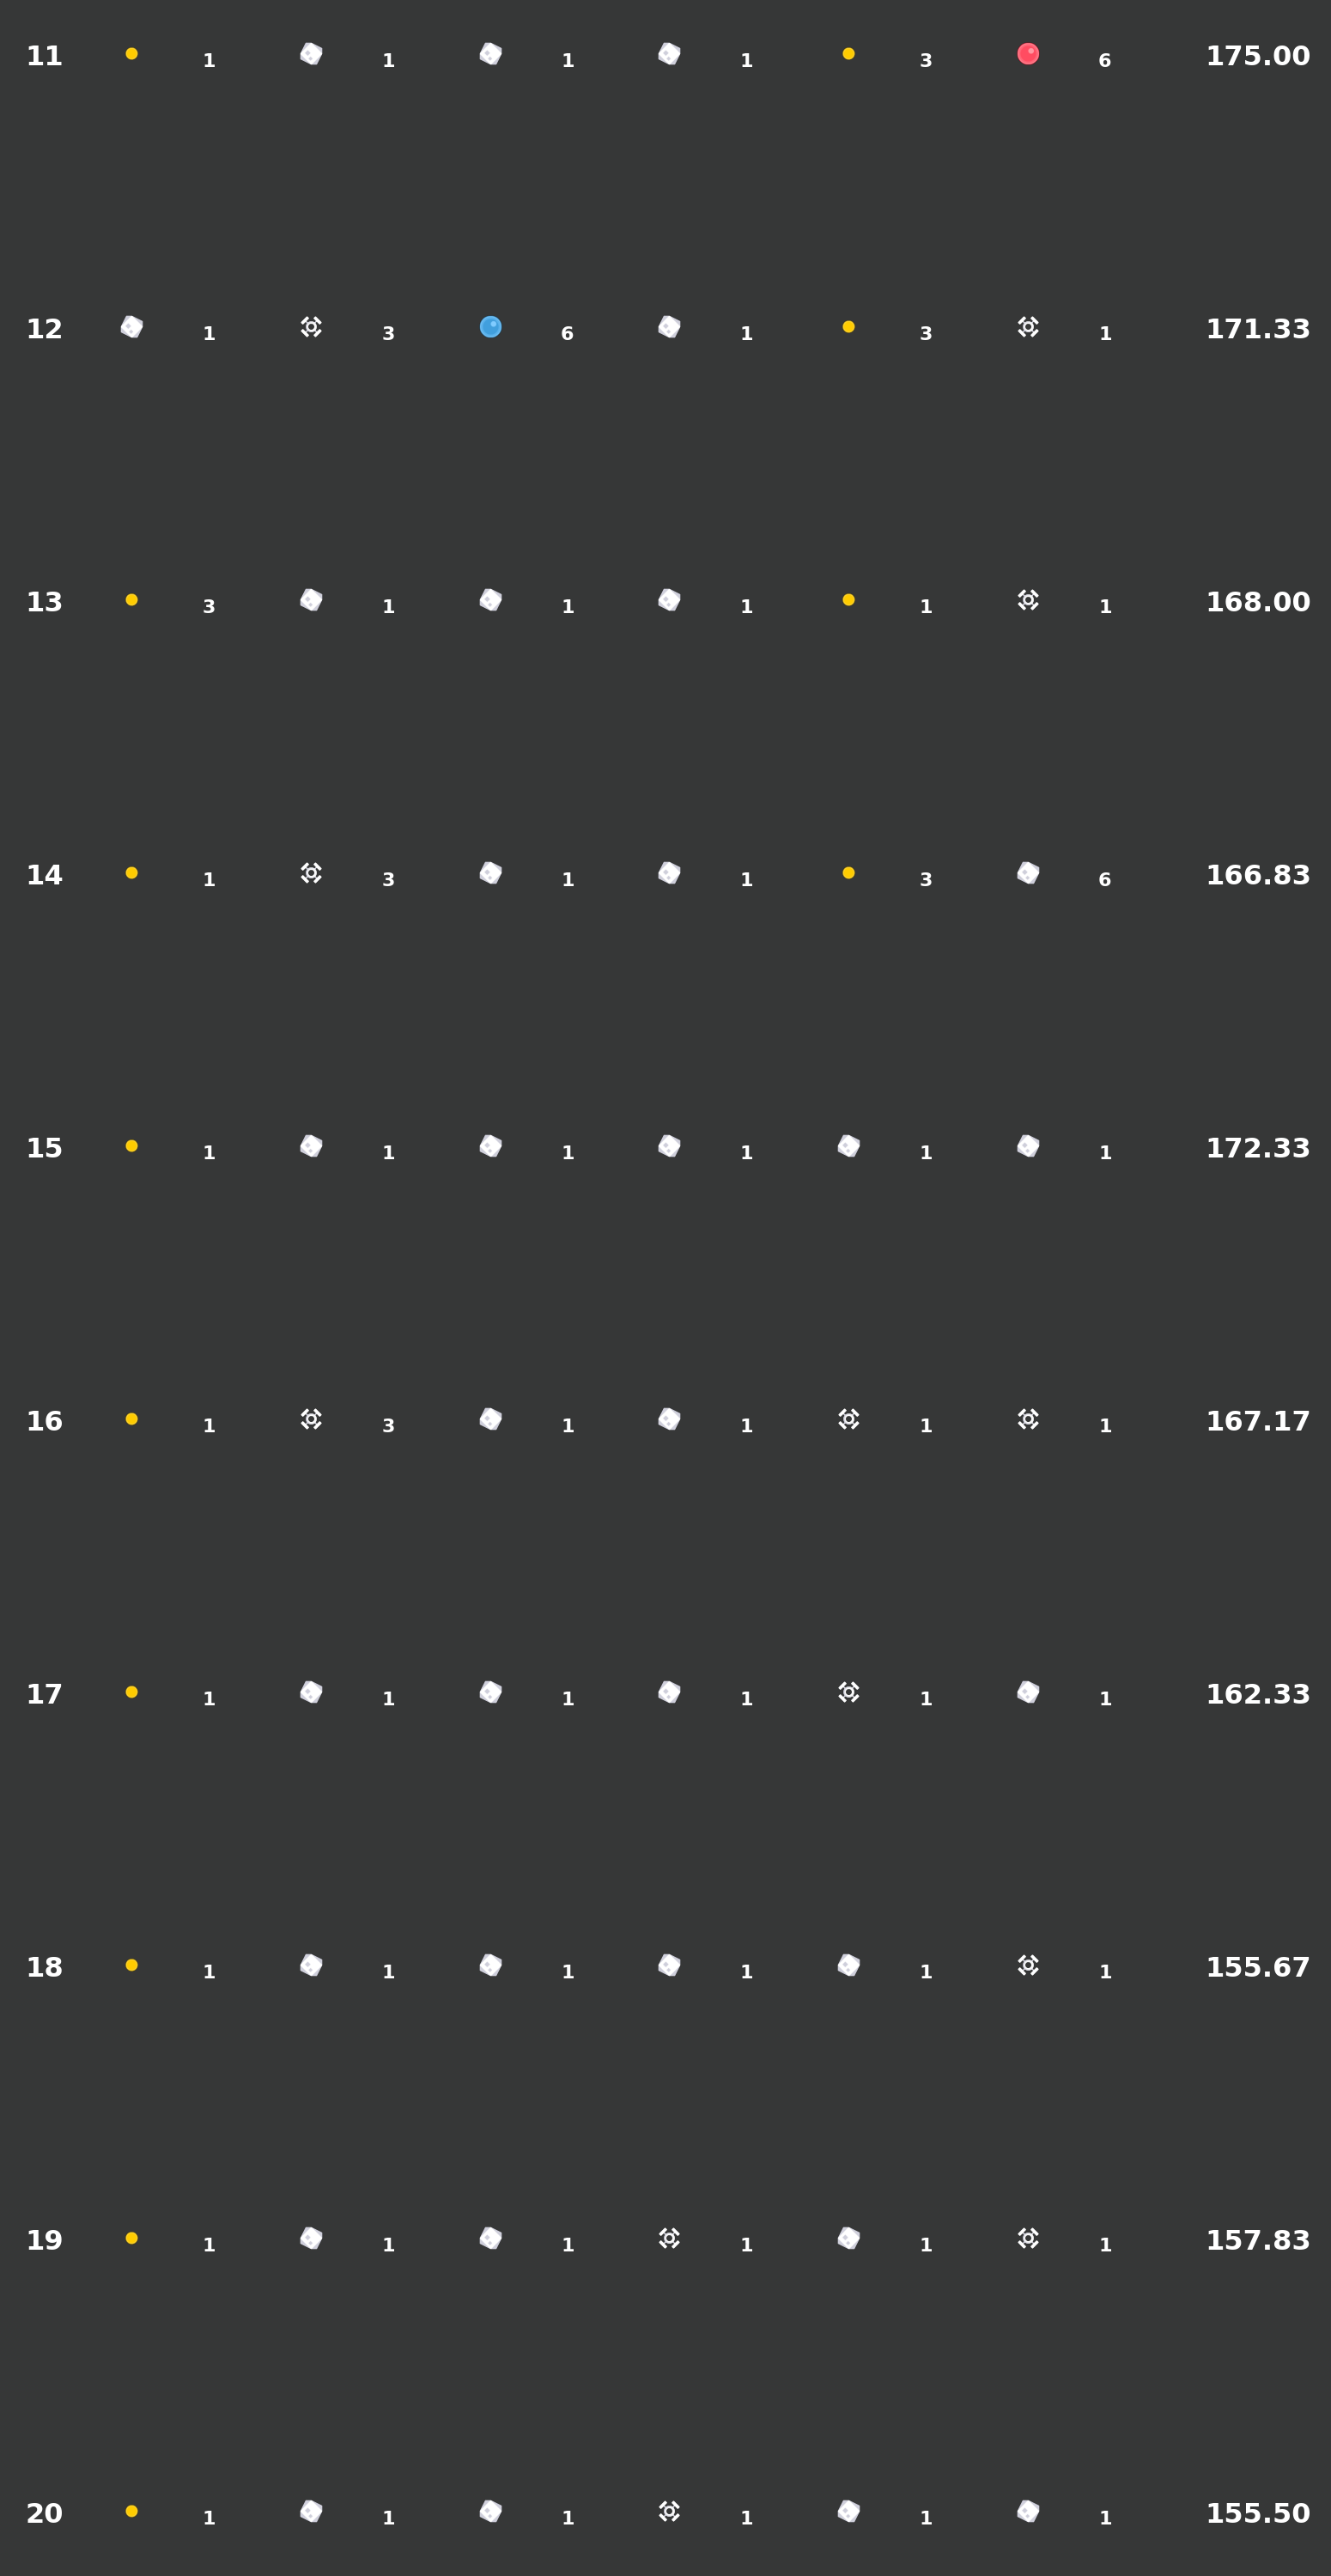
\includegraphics[width=0.7\textwidth]{figuras/ss/ss_yellowstill_ai_mode_1_2.png}
  \caption{Visualização da moda de cada onda com a versão v1 contra Nave Movendo, Disparo Amarelo.}
  \label{fig:ss-moda-ym-1-2}
\end{figure}

\begin{figure}[H]
  \centering
  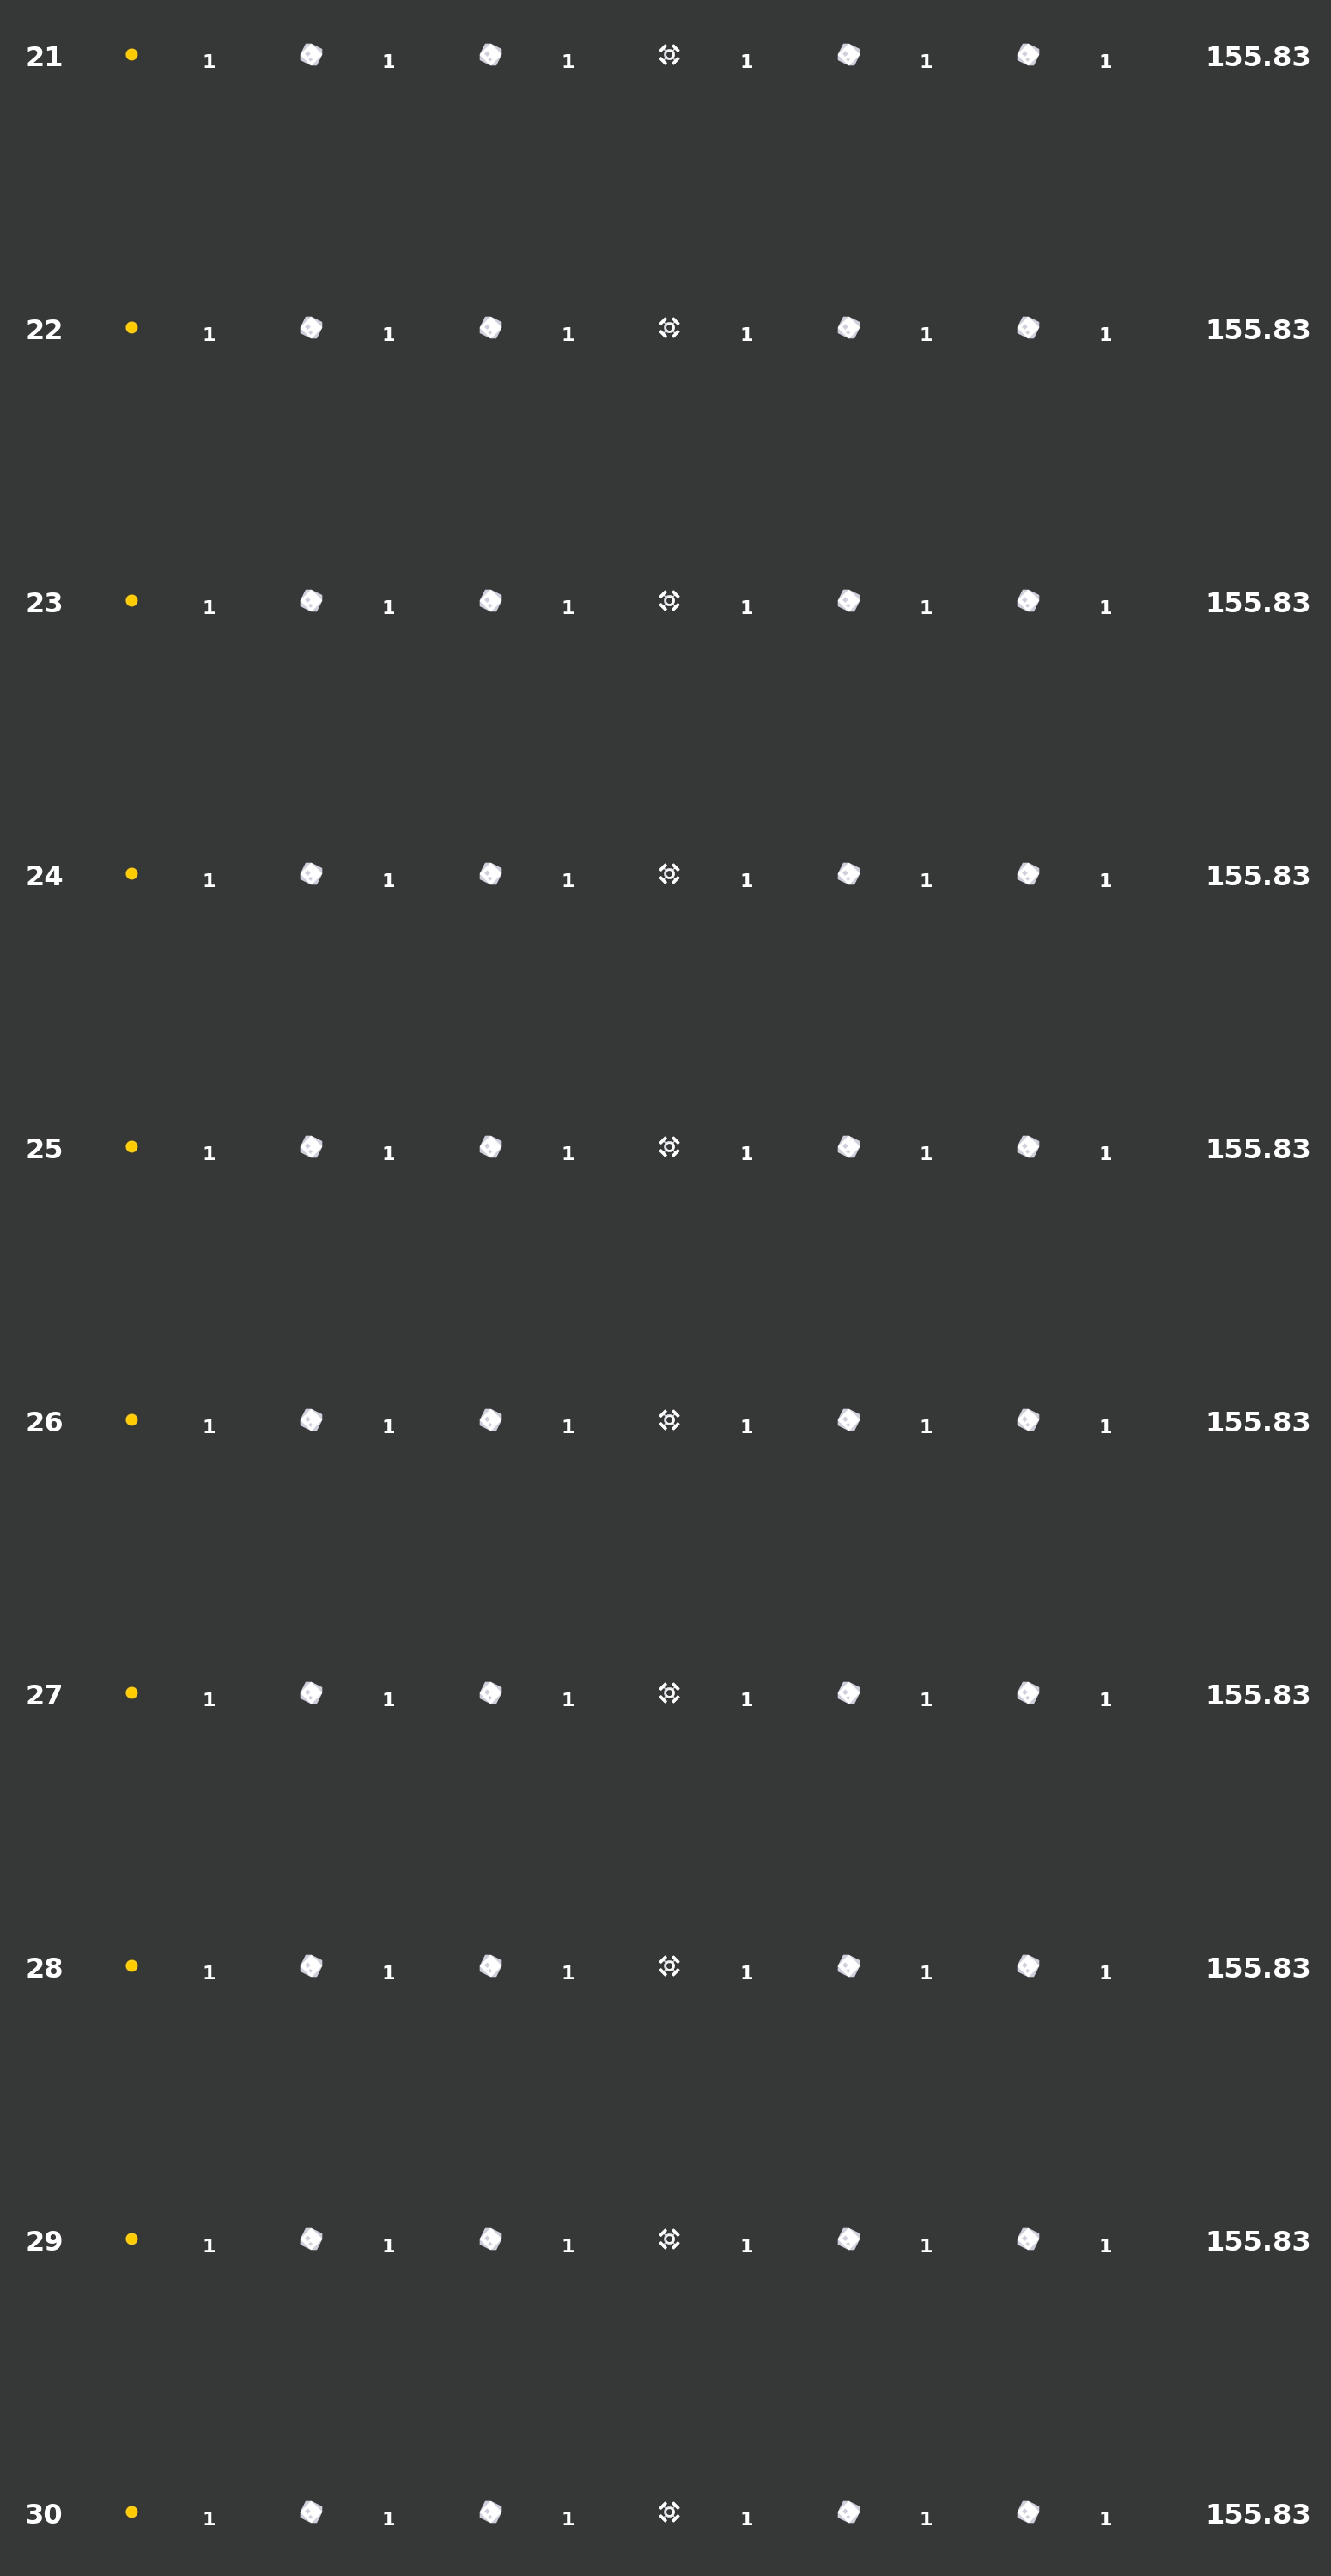
\includegraphics[width=0.7\textwidth]{figuras/ss/ss_yellowstill_ai_mode_1_3.png}
  \caption{Visualização da moda de cada onda com a versão v1 contra Nave Movendo, Disparo Amarelo.}
  \label{fig:ss-moda-ym-1-3}
\end{figure}

%% ------------------------------------------------------------------------- %%
\section{Nave Parada com Disparo Vermelho}
\label{sec:apend-moda-ss-rs-v1}

\begin{figure}[H]
  \centering
  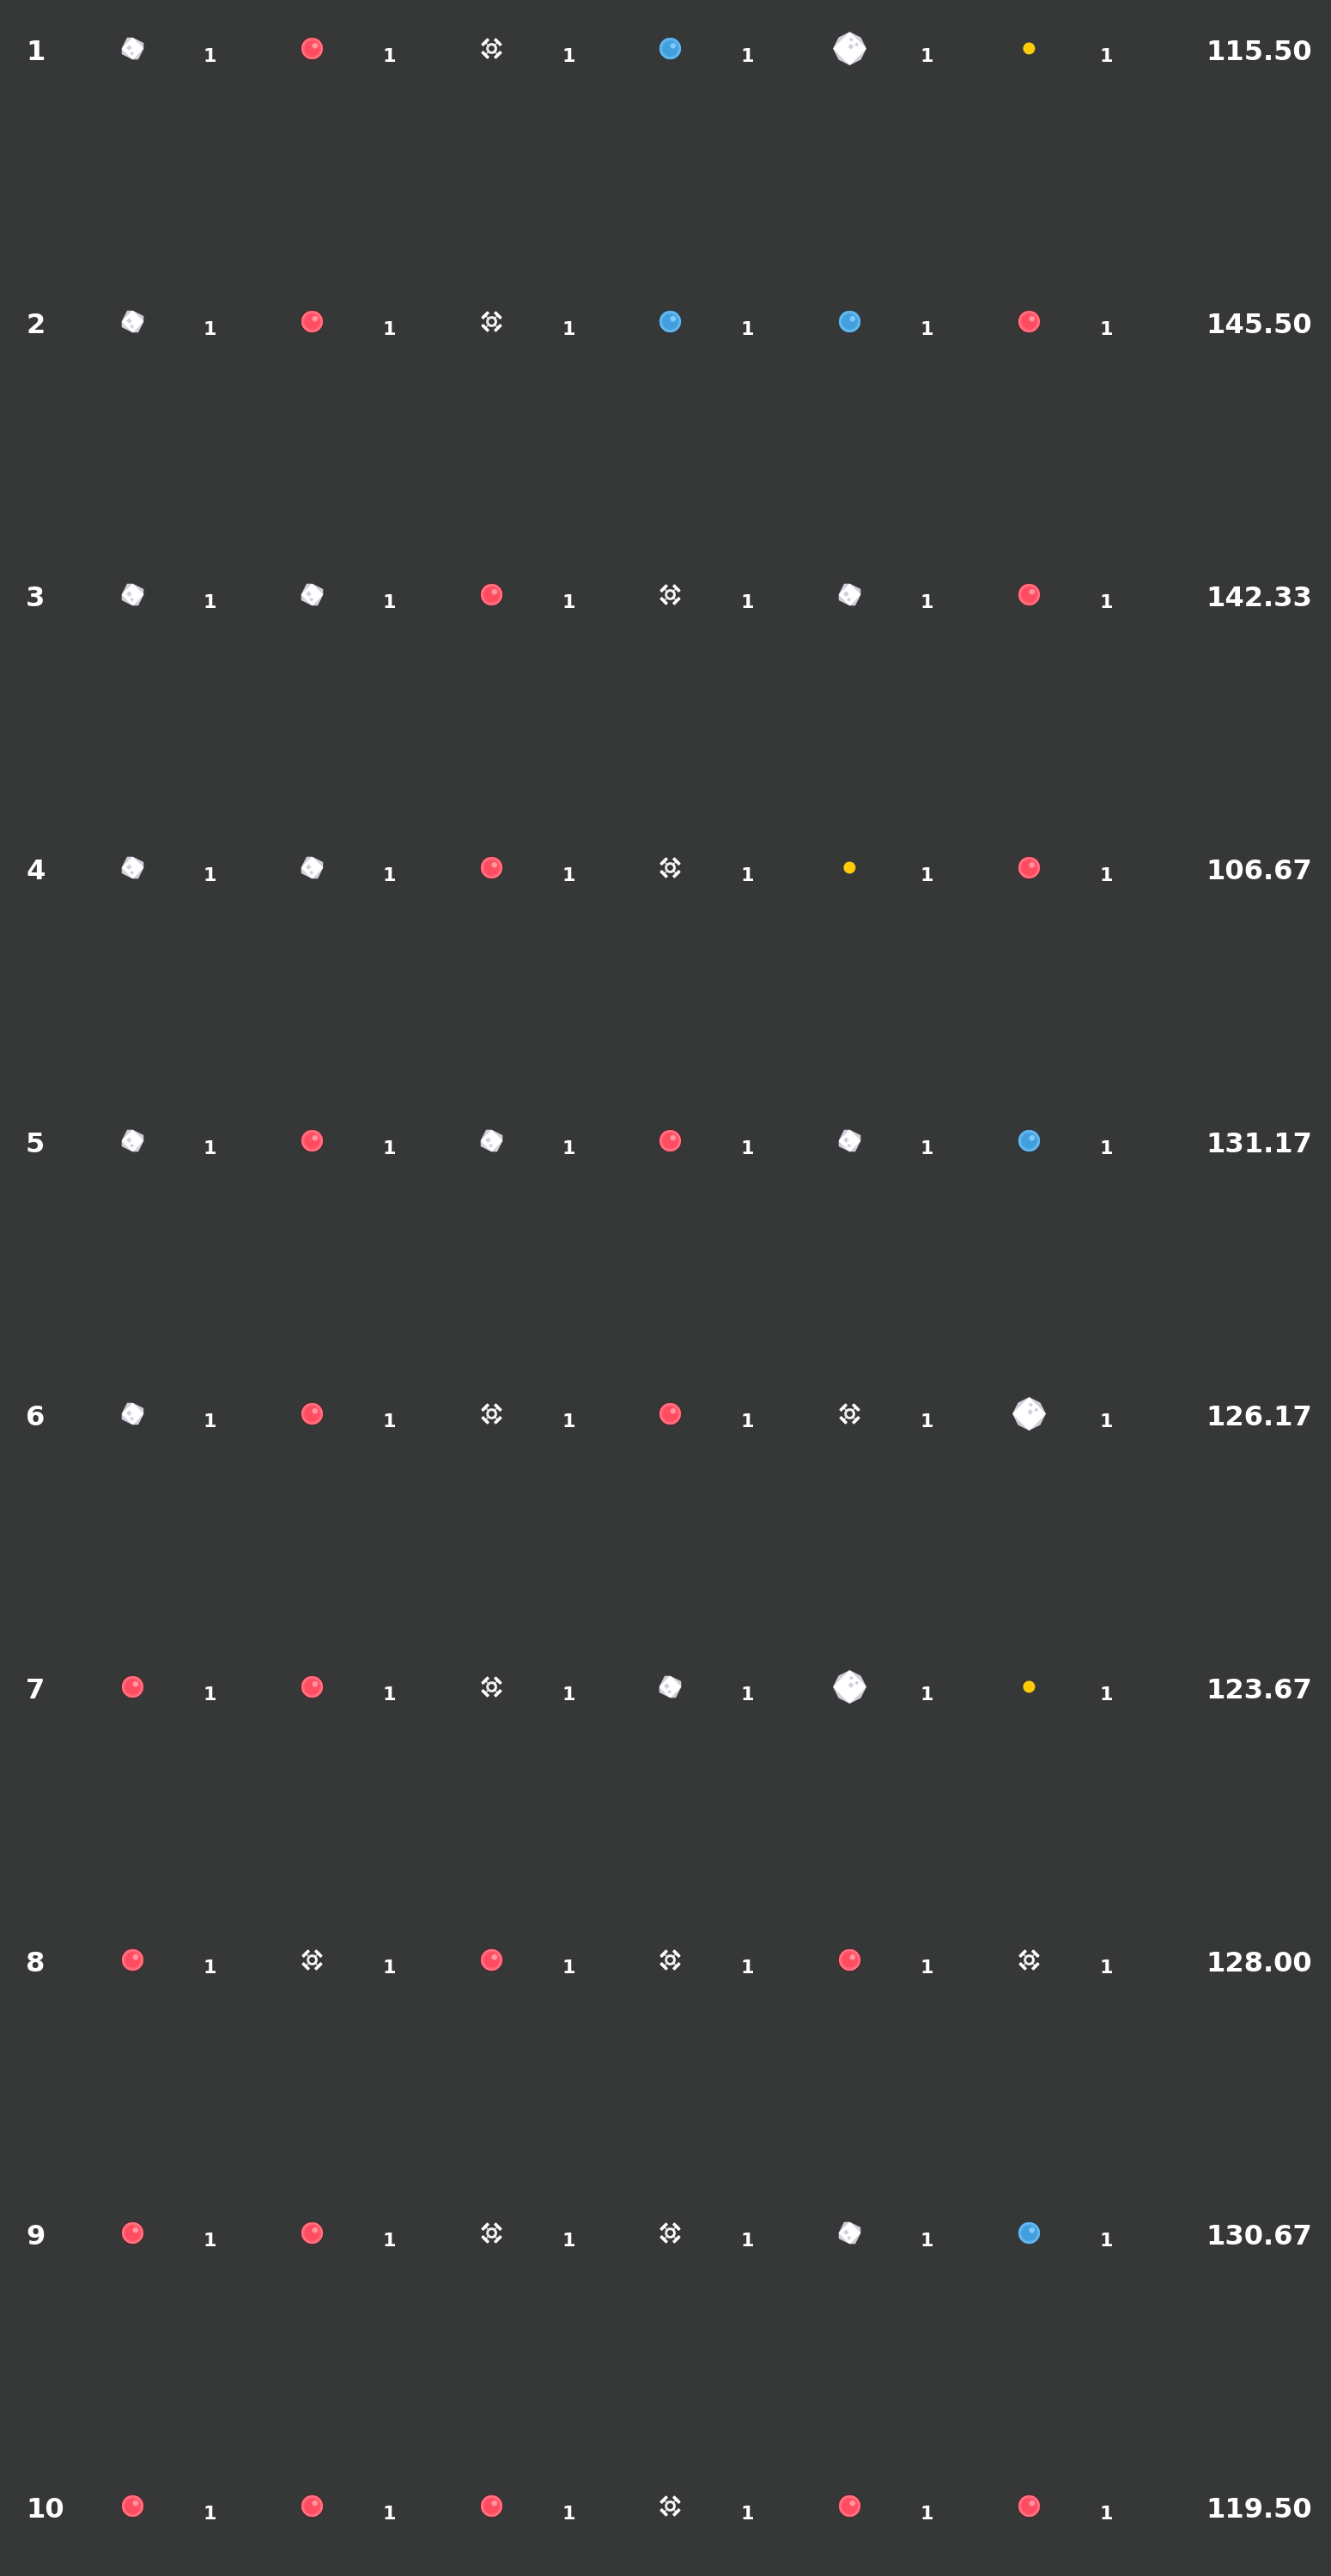
\includegraphics[width=0.7\textwidth]{figuras/ss/ss_redstill_ai_mode_1_1.png}
  \caption{Visualização da moda de cada onda com a versão v1 contra Nave Parada, Disparo Vermelho.}
  \label{fig:ss-moda-rs-1-1}
\end{figure}

\begin{figure}[H]
  \centering
  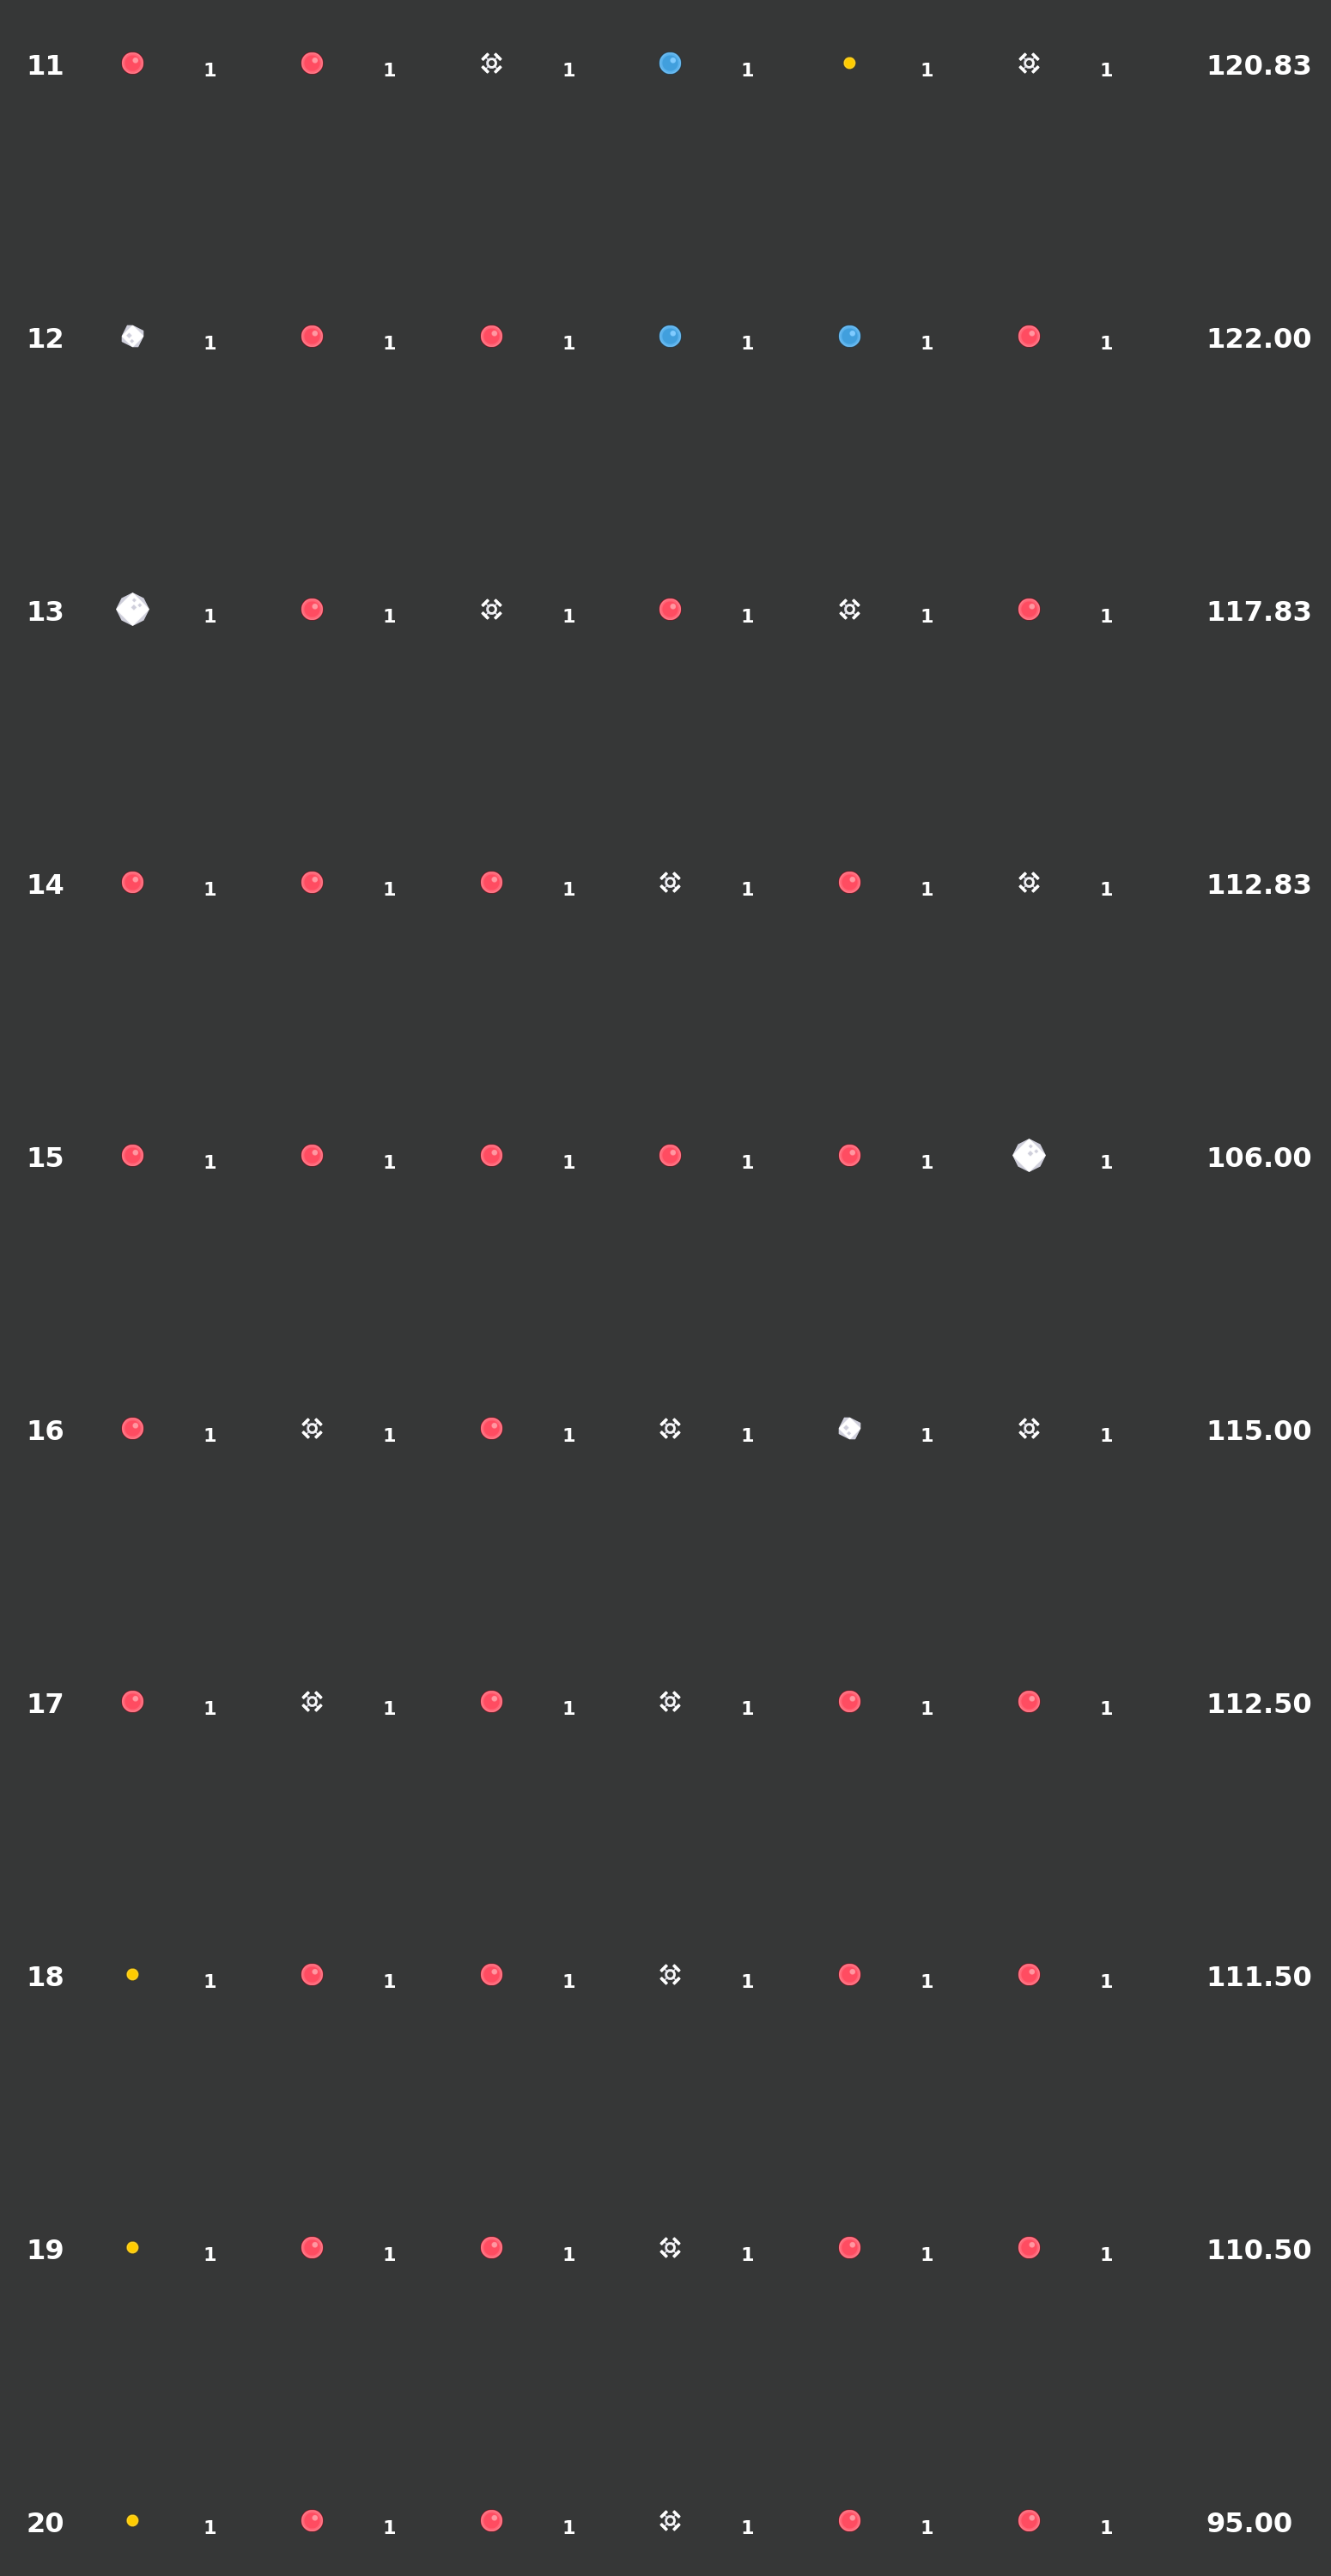
\includegraphics[width=0.7\textwidth]{figuras/ss/ss_redstill_ai_mode_1_2.png}
  \caption{Visualização da moda de cada onda com a versão v1 contra Nave Parada, Disparo Vermelho.}
  \label{fig:ss-moda-rs-1-2}
\end{figure}

\begin{figure}[H]
  \centering
  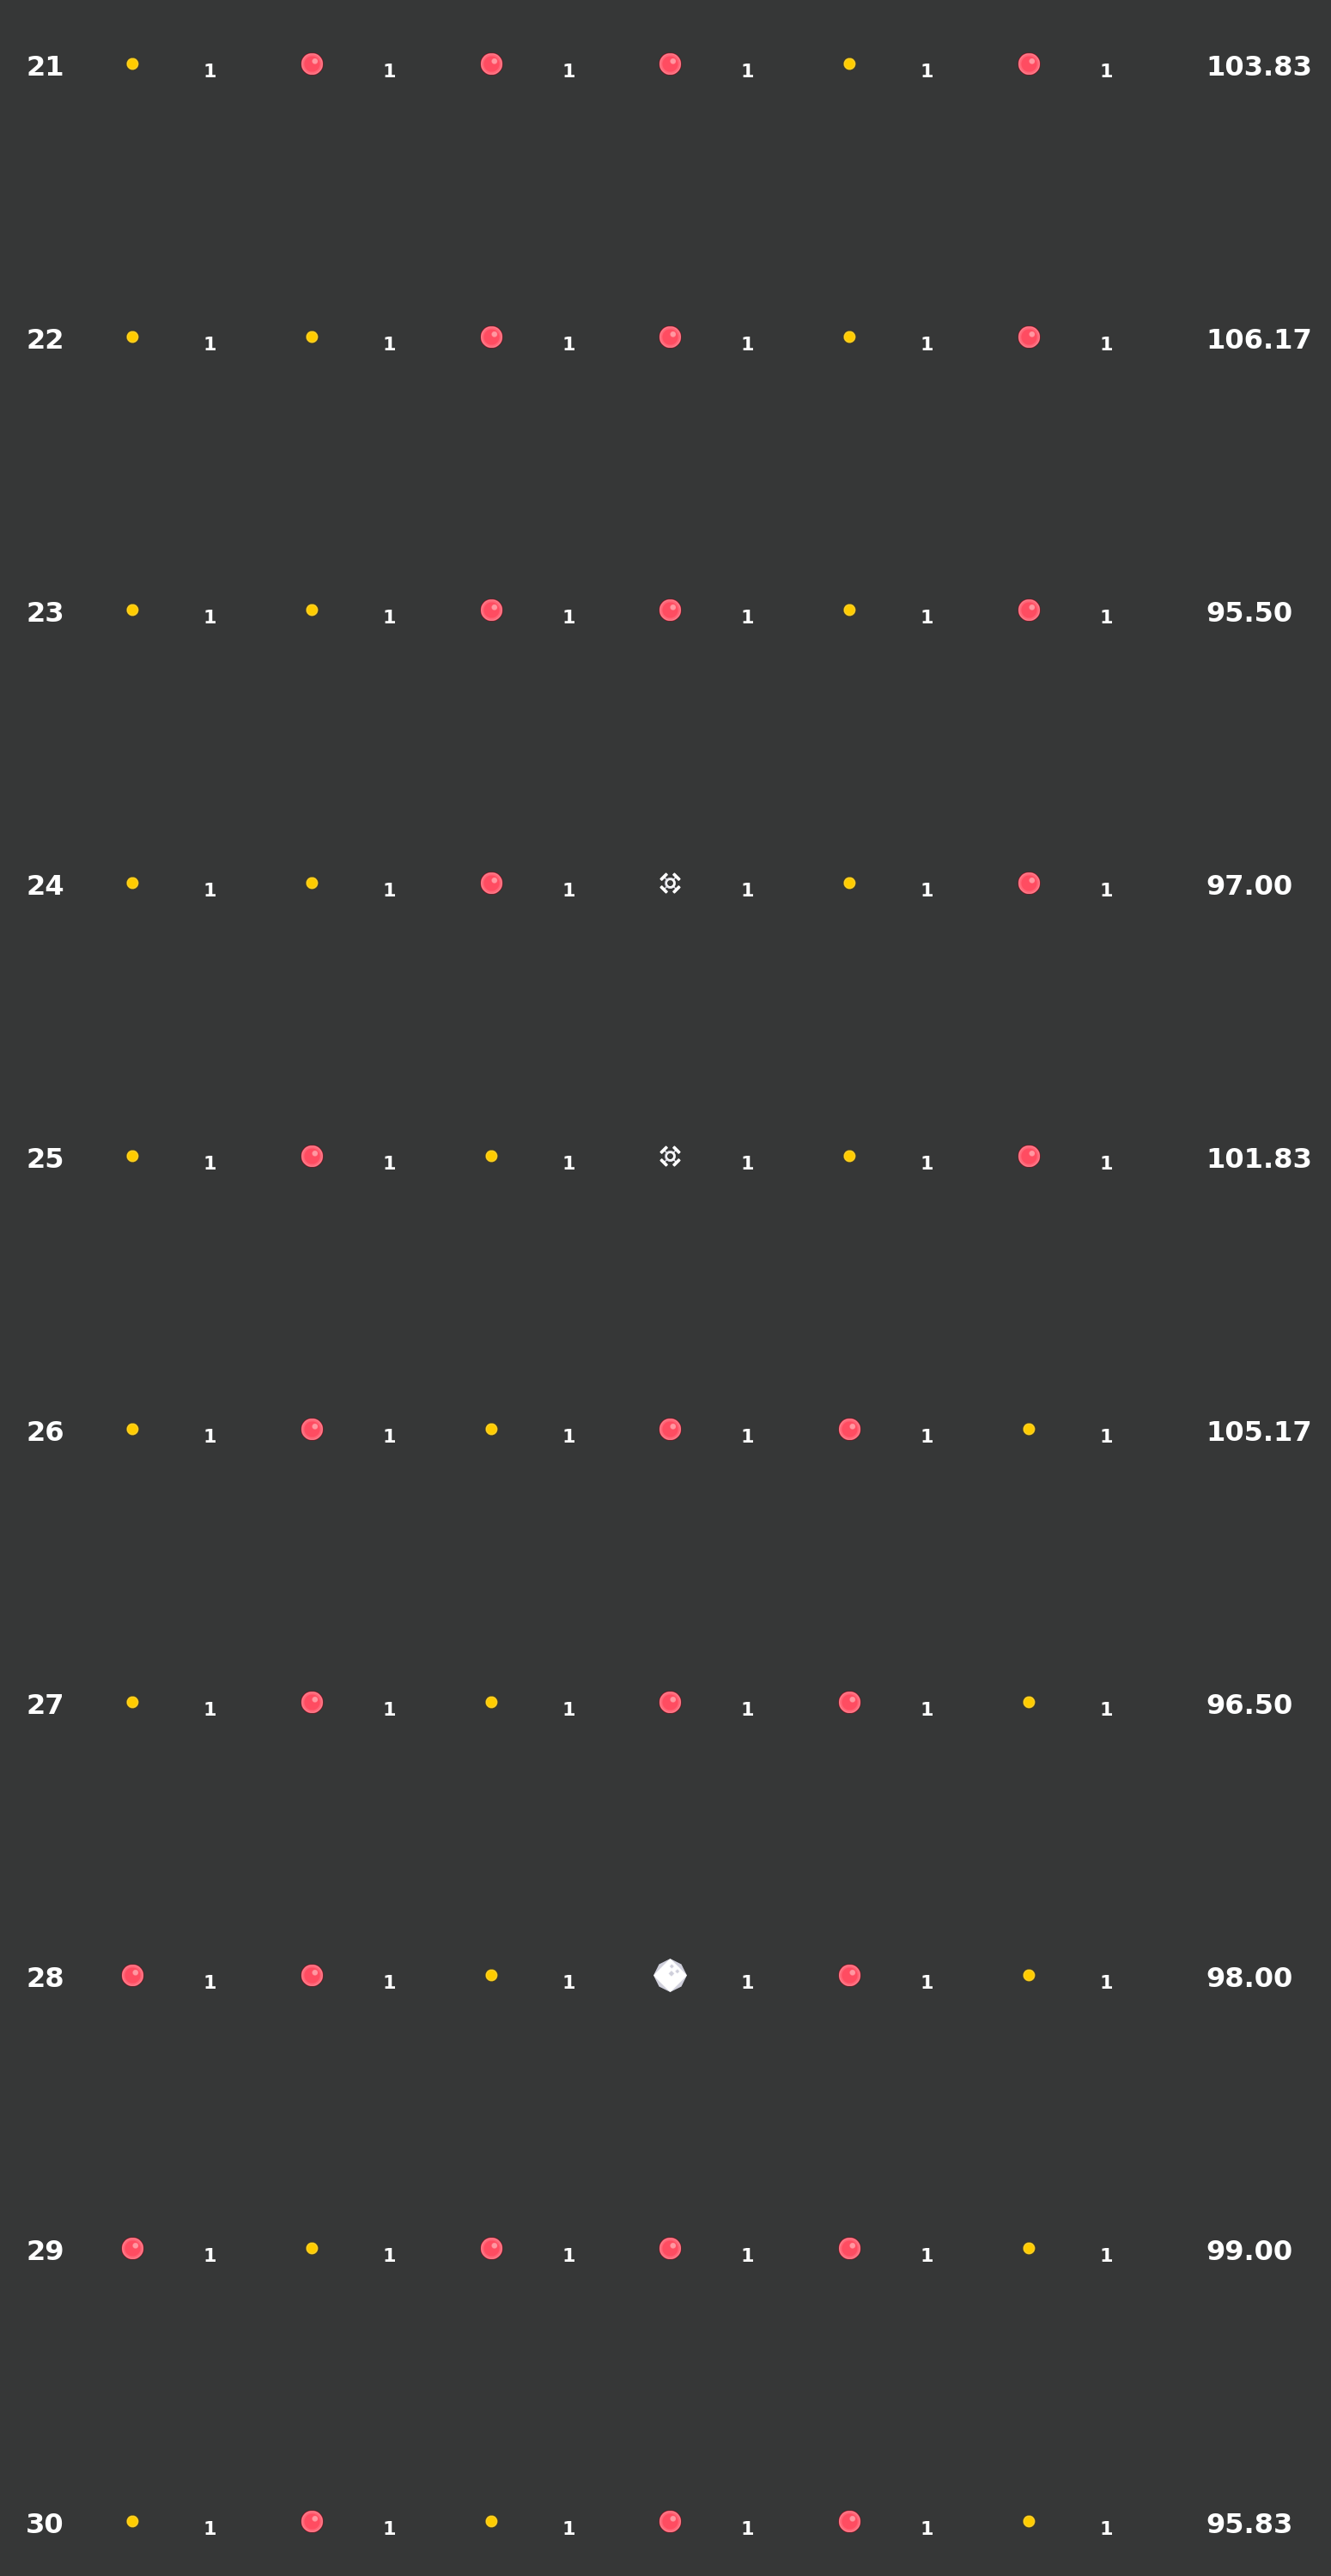
\includegraphics[width=0.7\textwidth]{figuras/ss/ss_redstill_ai_mode_1_3.png}
  \caption{Visualização da moda de cada onda com a versão v1 contra Nave Parada, Disparo Vermelho.}
  \label{fig:ss-moda-rs-1-3}
\end{figure}

%% ------------------------------------------------------------------------- %%
\section{Nave Movendo com Disparo Vermelho}
\label{sec:apend-moda-ss-rm-v1}

\begin{figure}[H]
  \centering
  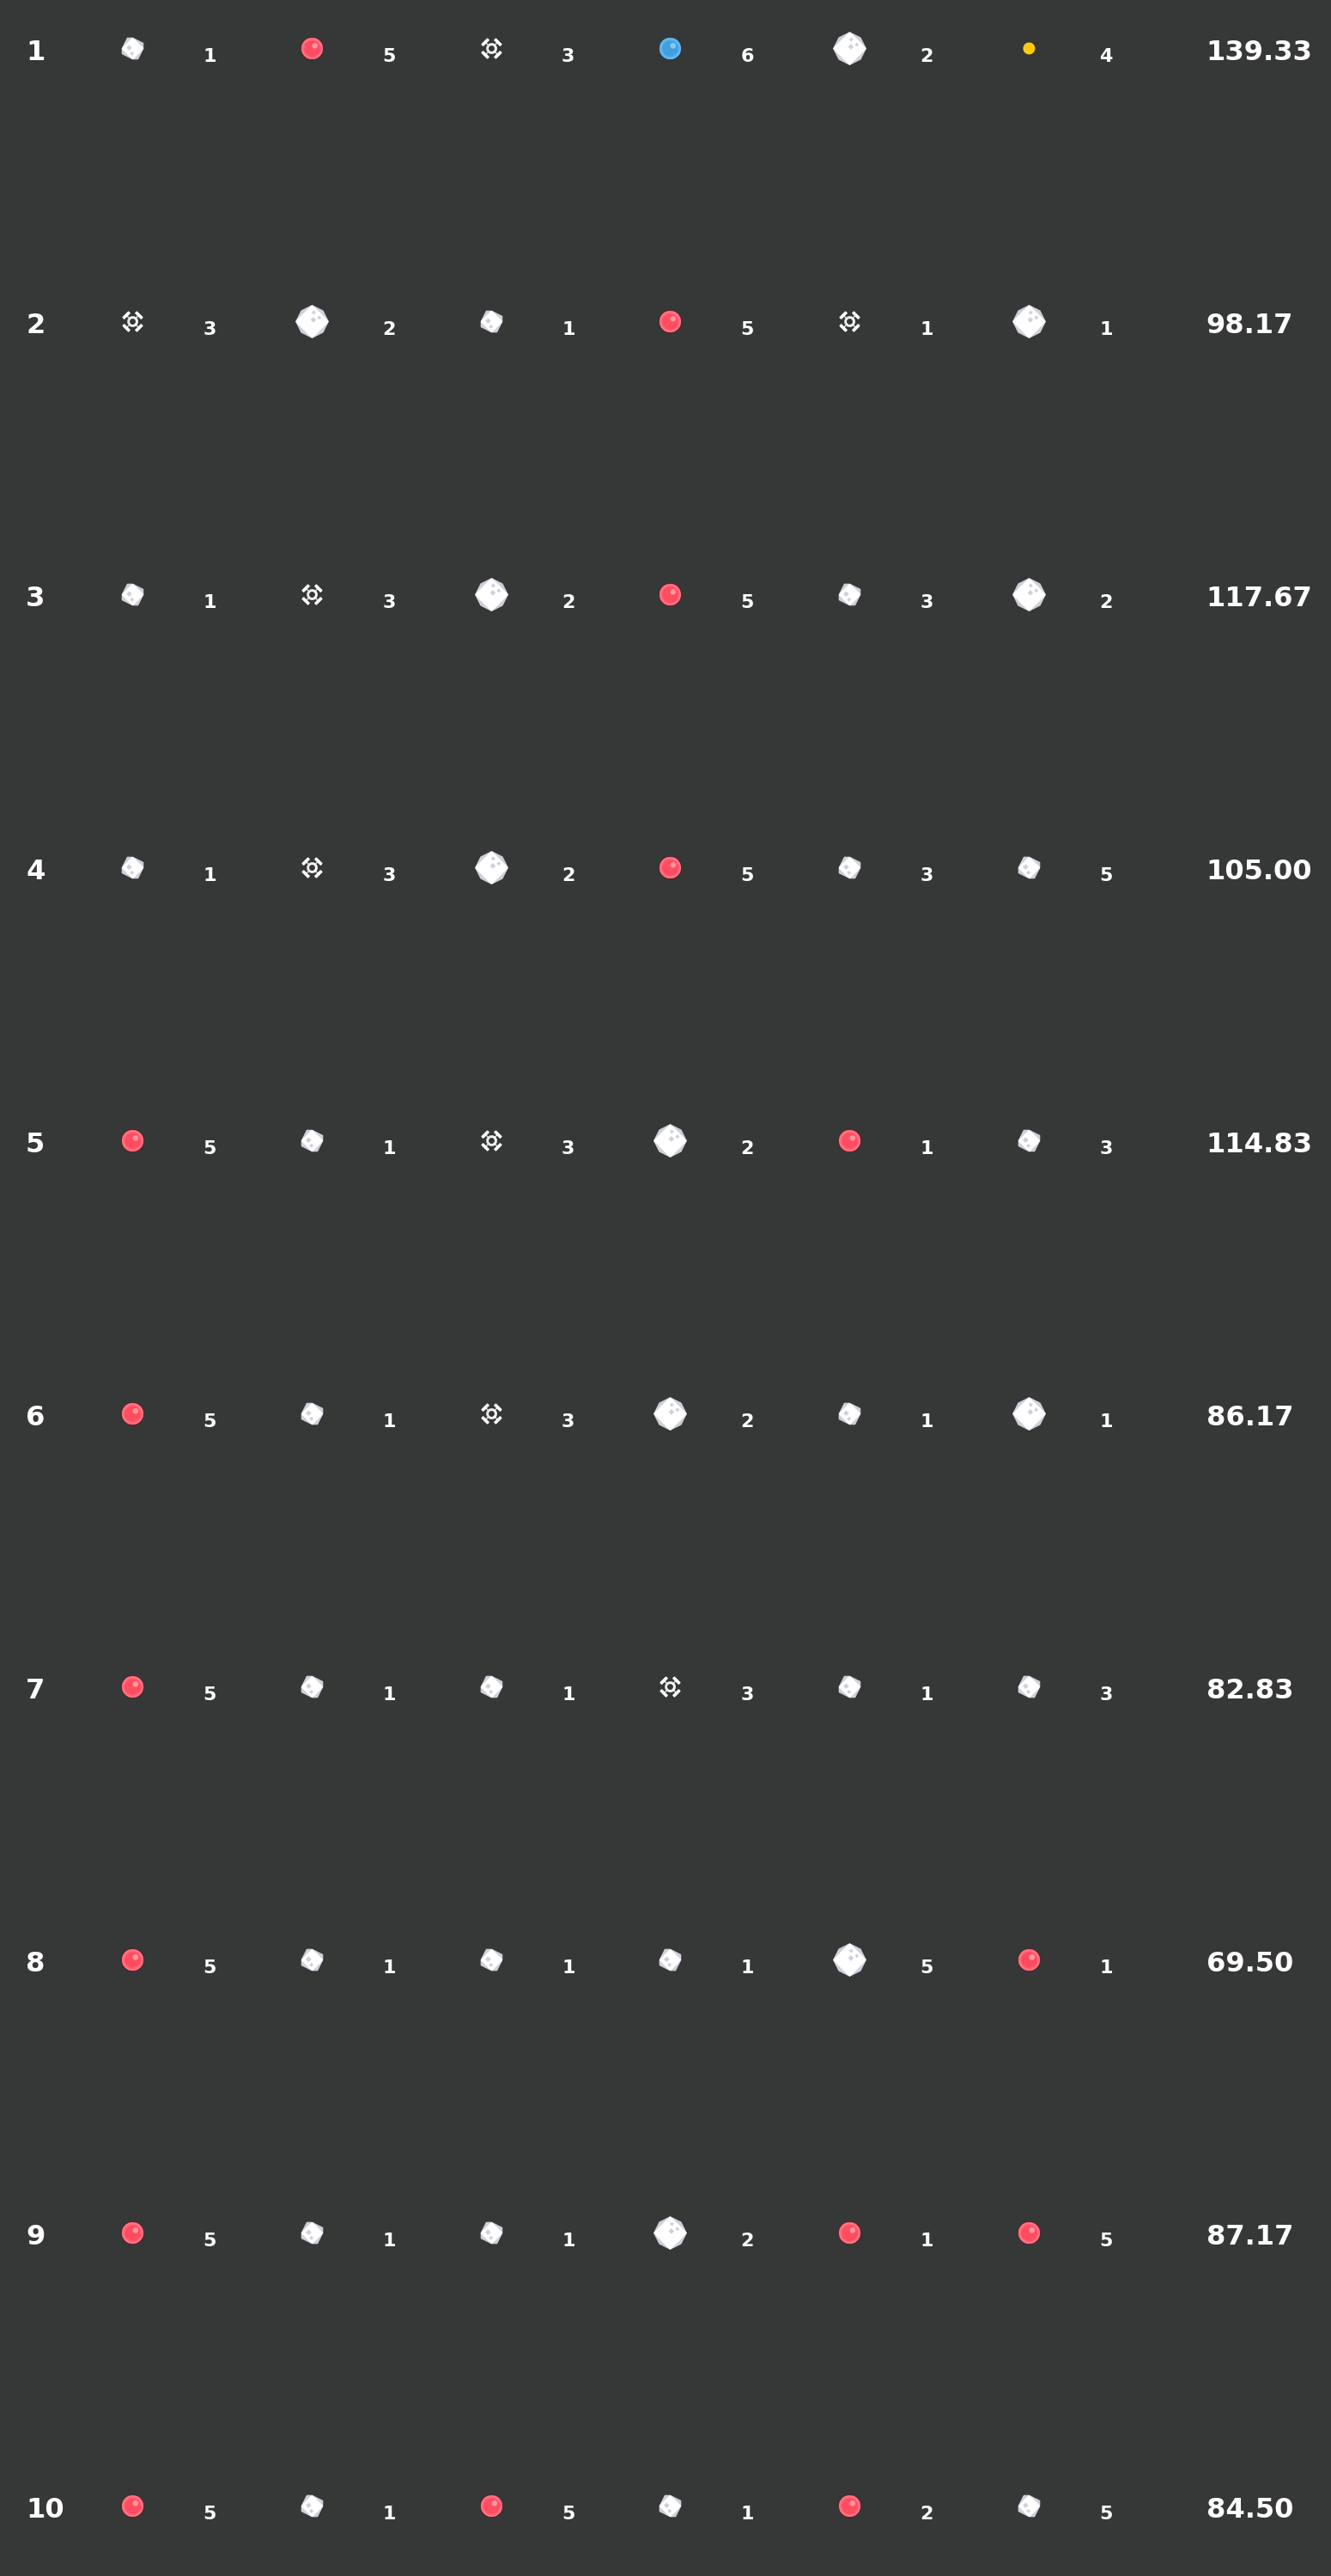
\includegraphics[width=0.7\textwidth]{figuras/ss/ss_redmove_ai_mode_1_1.png}
  \caption{Visualização da moda de cada onda com a versão v1 contra Nave Movendo, Disparo Vermelho.}
  \label{fig:ss-moda-rm-1-1}
\end{figure}

\begin{figure}[H]
  \centering
  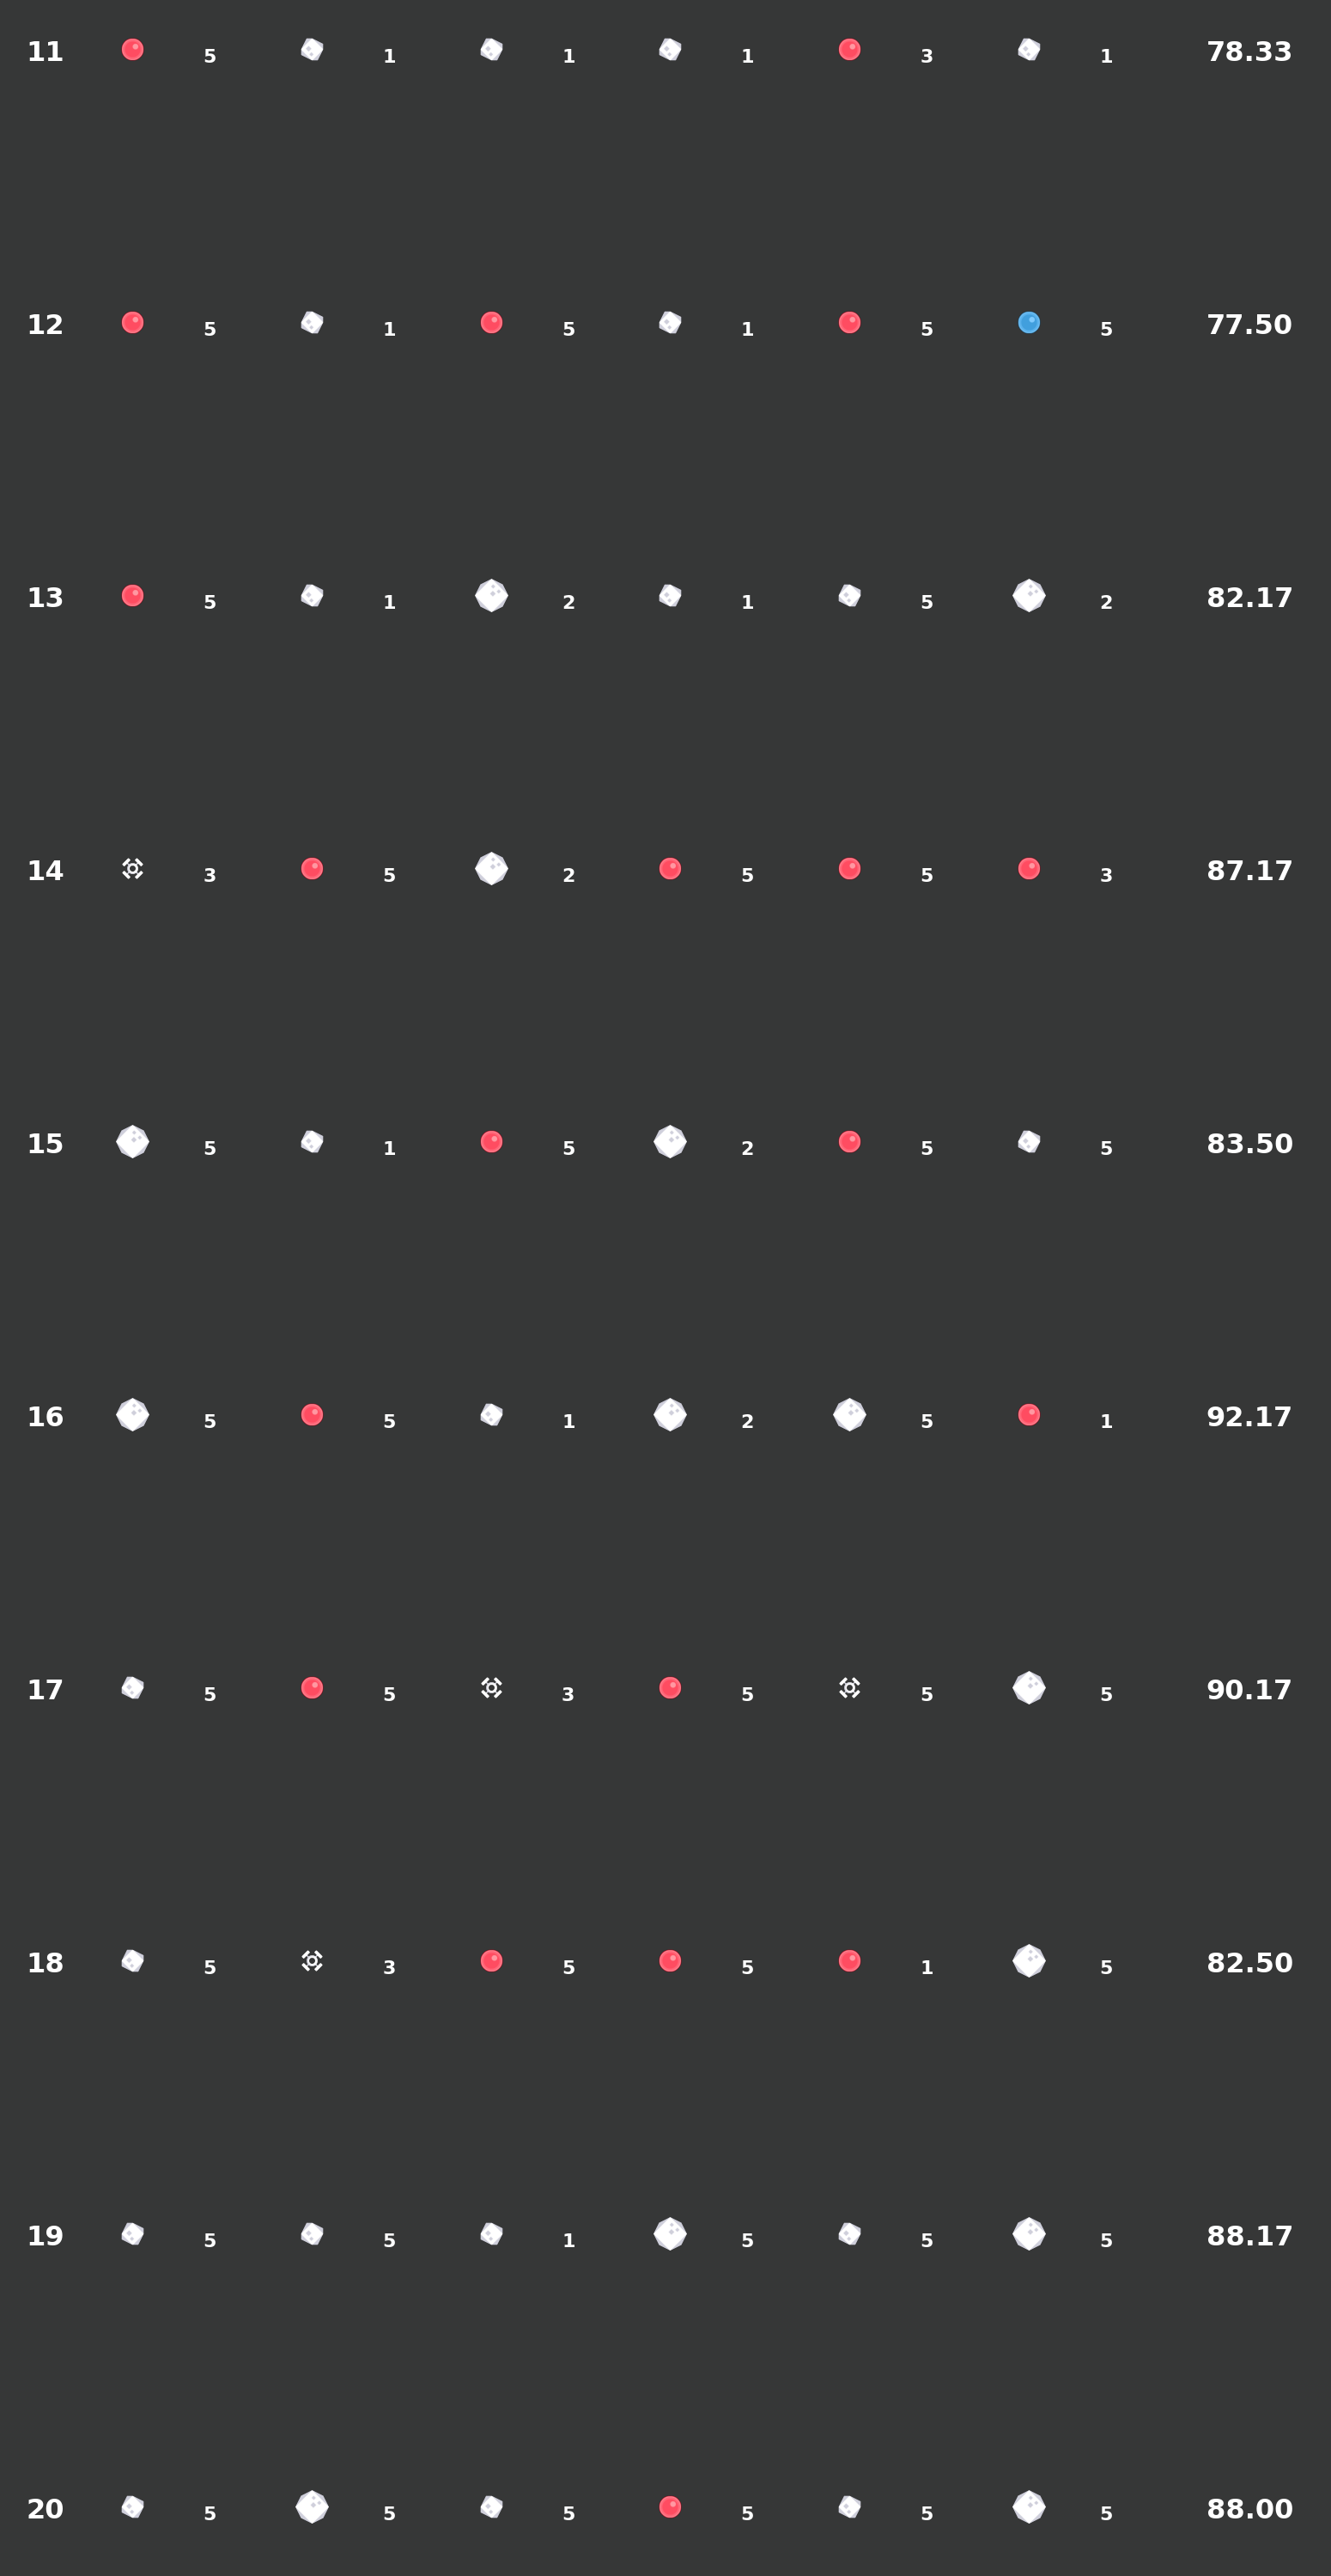
\includegraphics[width=0.7\textwidth]{figuras/ss/ss_redmove_ai_mode_1_2.png}
  \caption{Visualização da moda de cada onda com a versão v1 contra Nave Movendo, Disparo Vermelho.}
  \label{fig:ss-moda-rm-1-2}
\end{figure}

\begin{figure}[H]
  \centering
  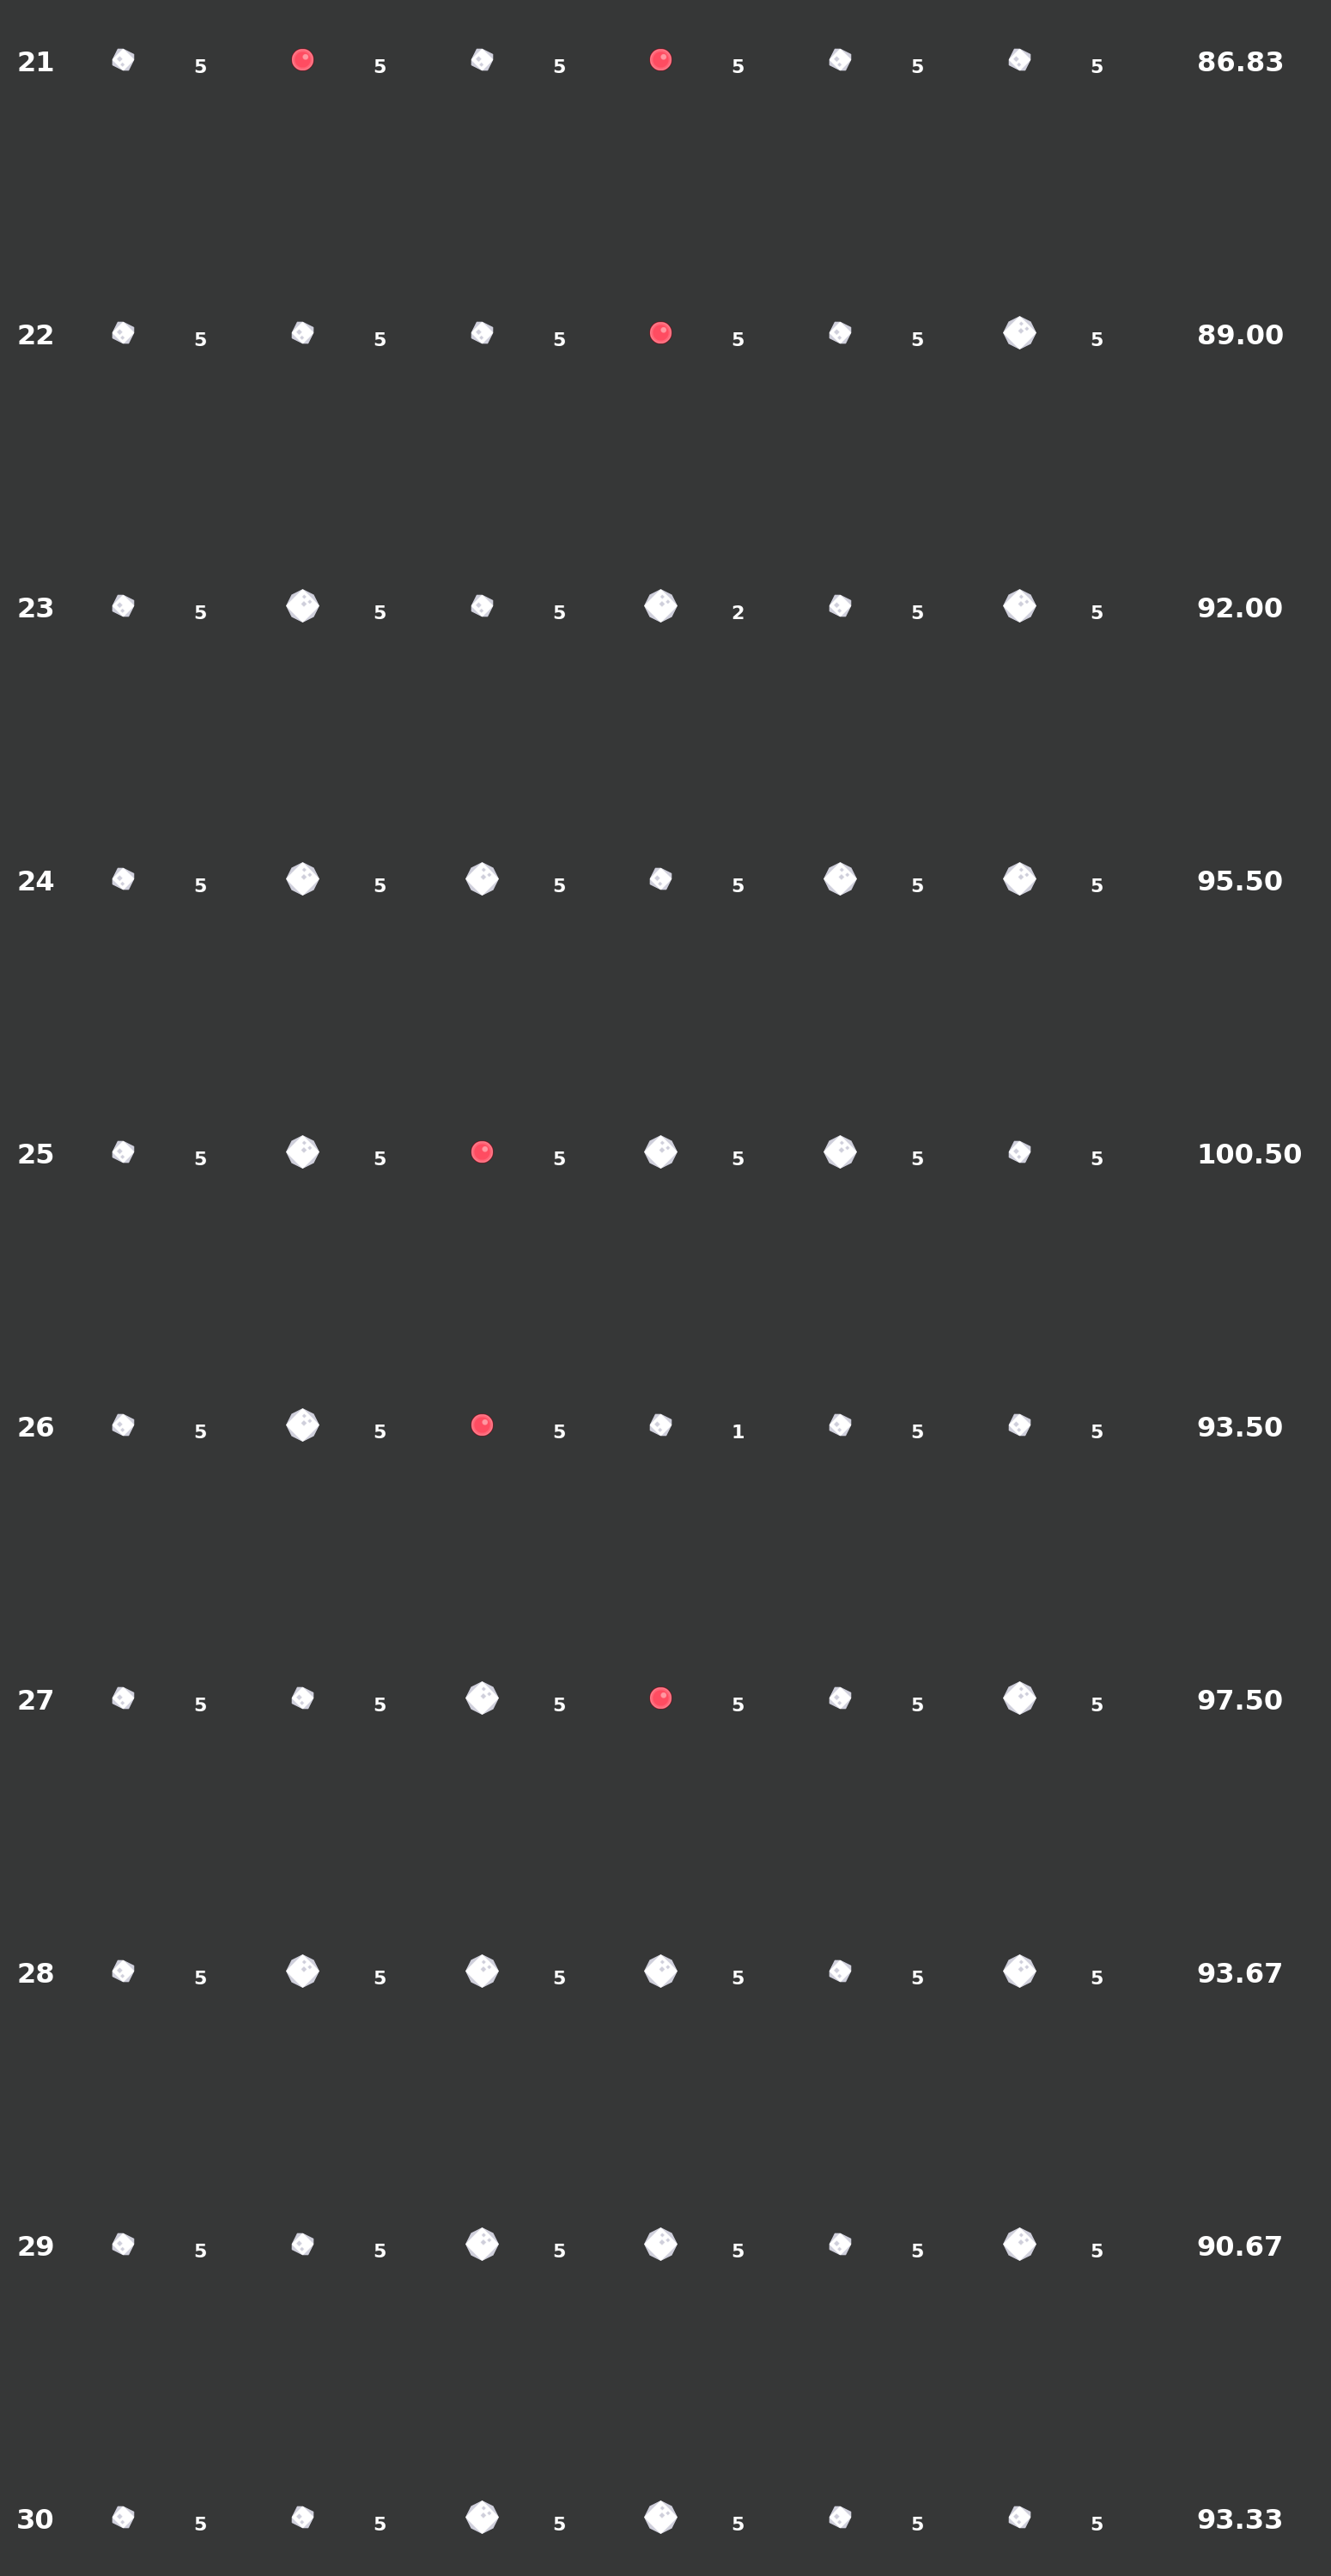
\includegraphics[width=0.7\textwidth]{figuras/ss/ss_redmove_ai_mode_1_3.png}
  \caption{Visualização da moda de cada onda com a versão v1 contra Nave Movendo, Disparo Vermelho.}
  \label{fig:ss-moda-rm-1-3}
\end{figure}
\par

%% ------------------------------------------------------------------------- %%
\chapter{Moda das Ondas no Space Shooter para versão v3}
\label{sec:apend-moda-ss-v3}

Foram calculadas as modas das ondas do \textit{fitness} desenvolvido, para permitir a visualização dos inimigos mais comuns que o algoritmo convergiu.

%% ------------------------------------------------------------------------- %%
\section{Nave Parada com Disparo Amarelo}
\label{sec:apend-moda-ss-ys-v3}

\begin{figure}[H]
  \centering
  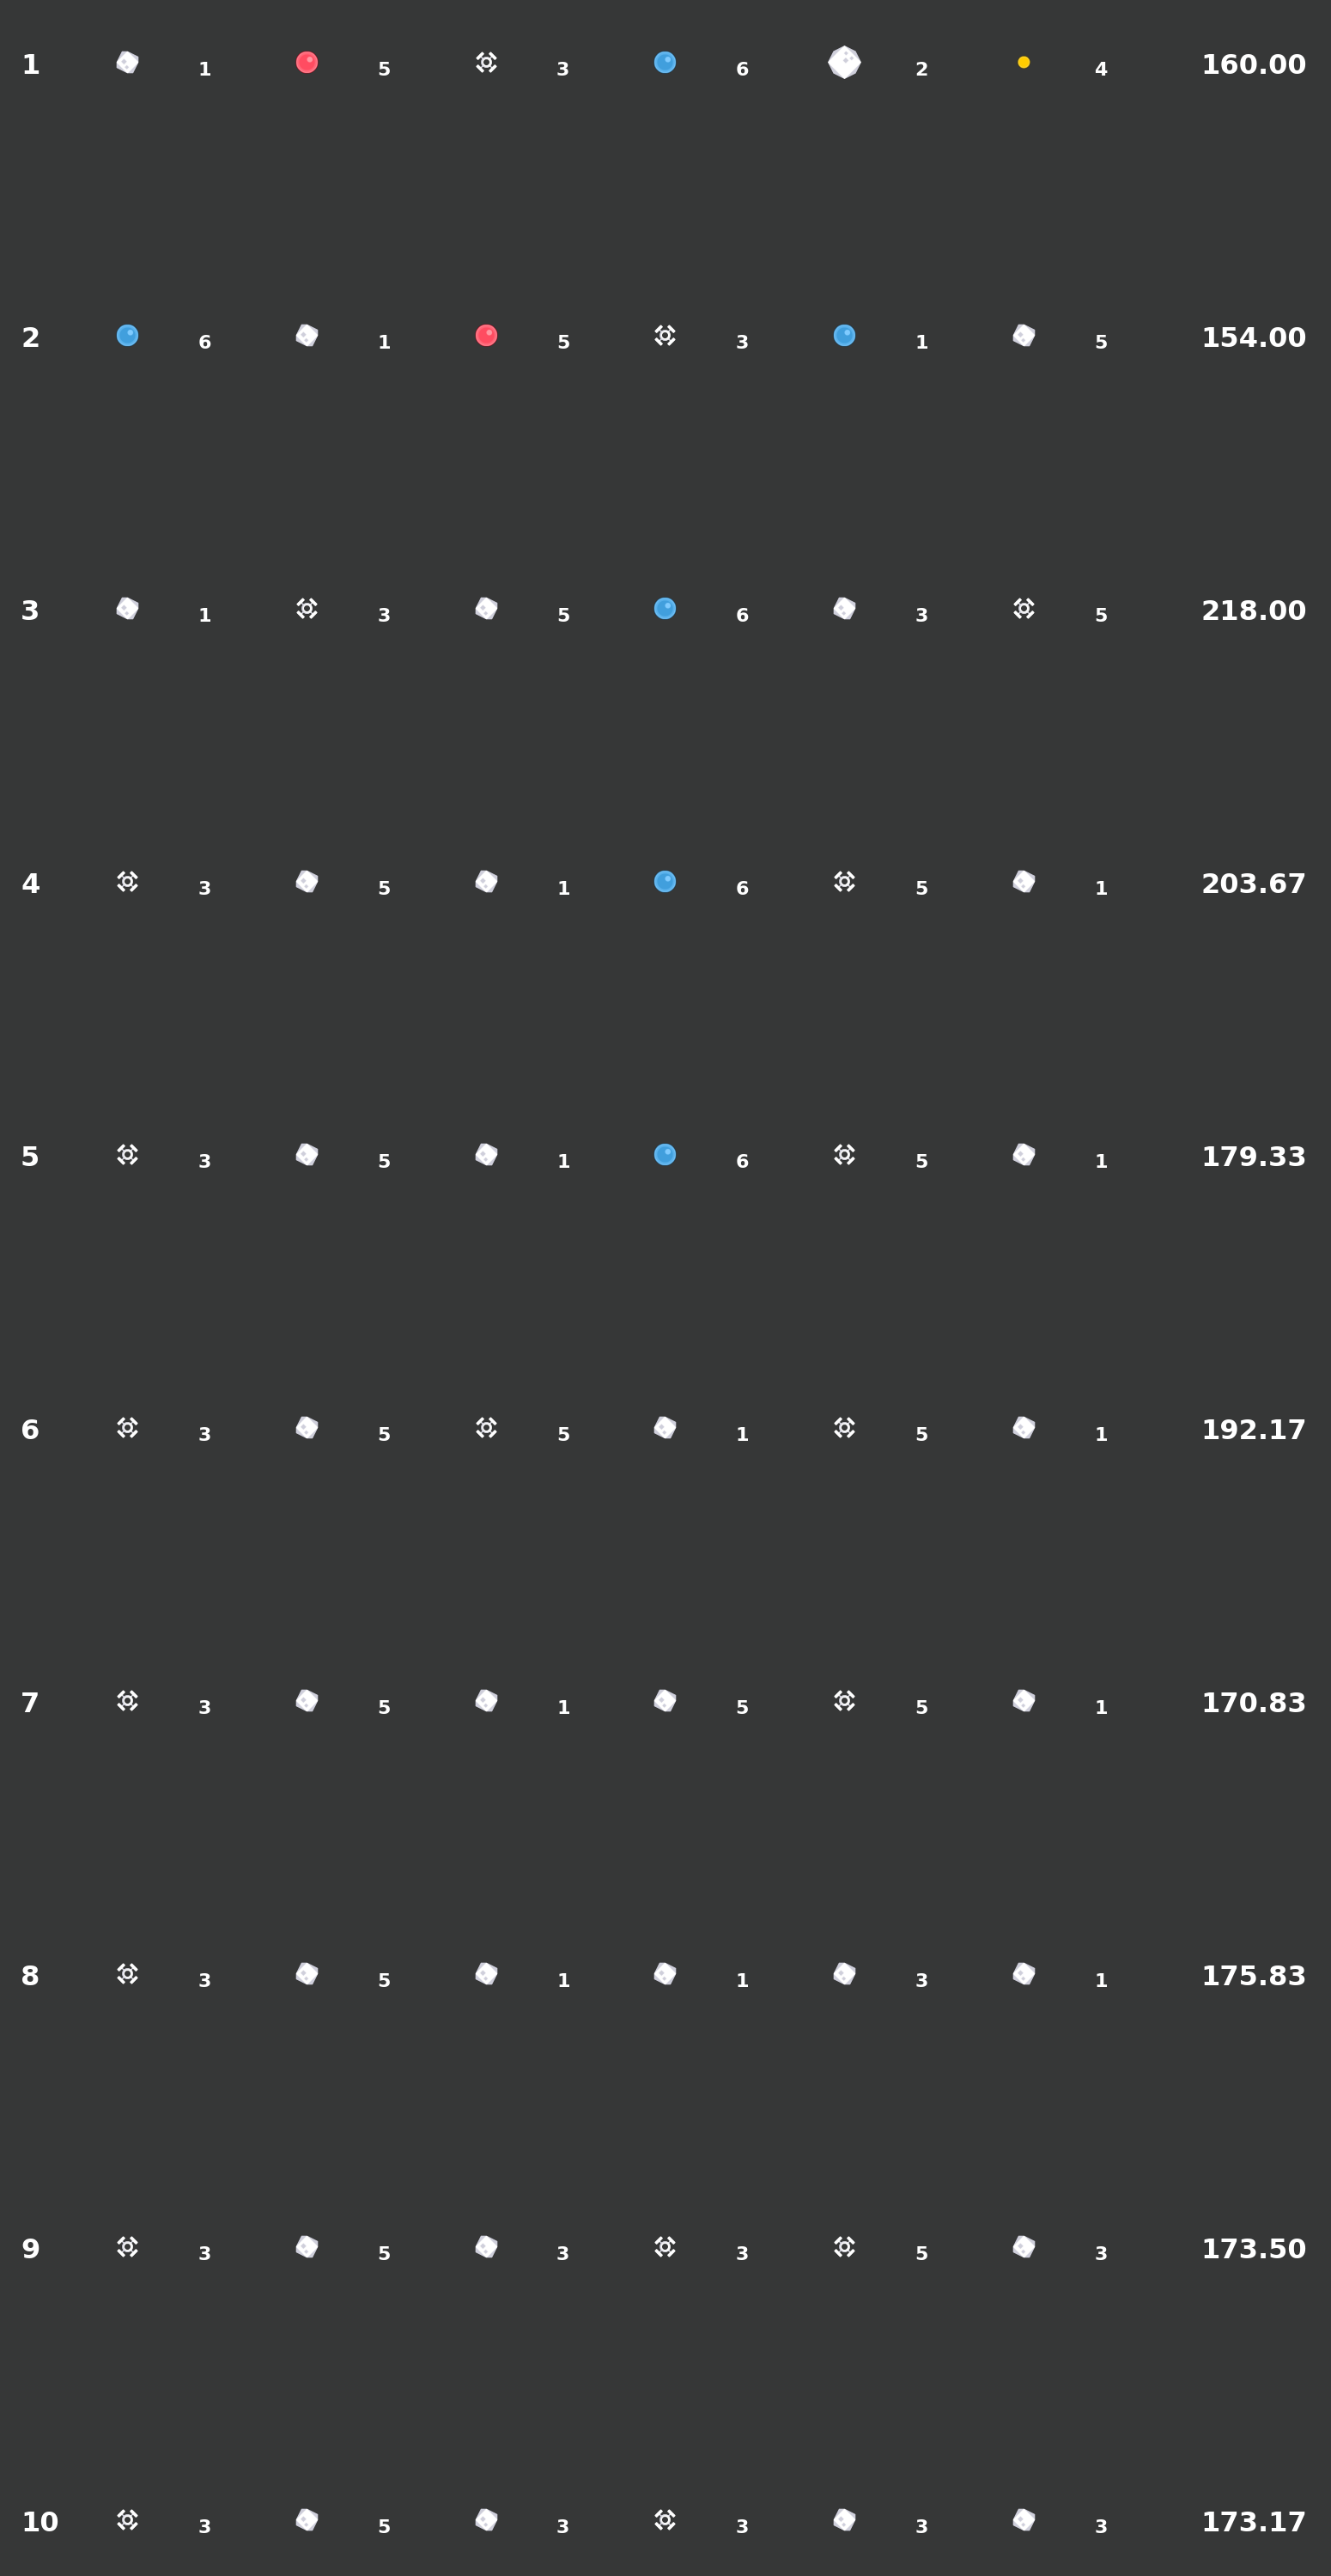
\includegraphics[width=0.7\textwidth]{figuras/ss/ss_yellowstill_ai_mode_2_1.png}
  \caption{Visualização da moda de cada onda com o fitness v3 contra Nave Parada, Disparo Amarelo.}
  \label{fig:ss-moda-ys-2-1}
\end{figure}

\begin{figure}[H]
  \centering
  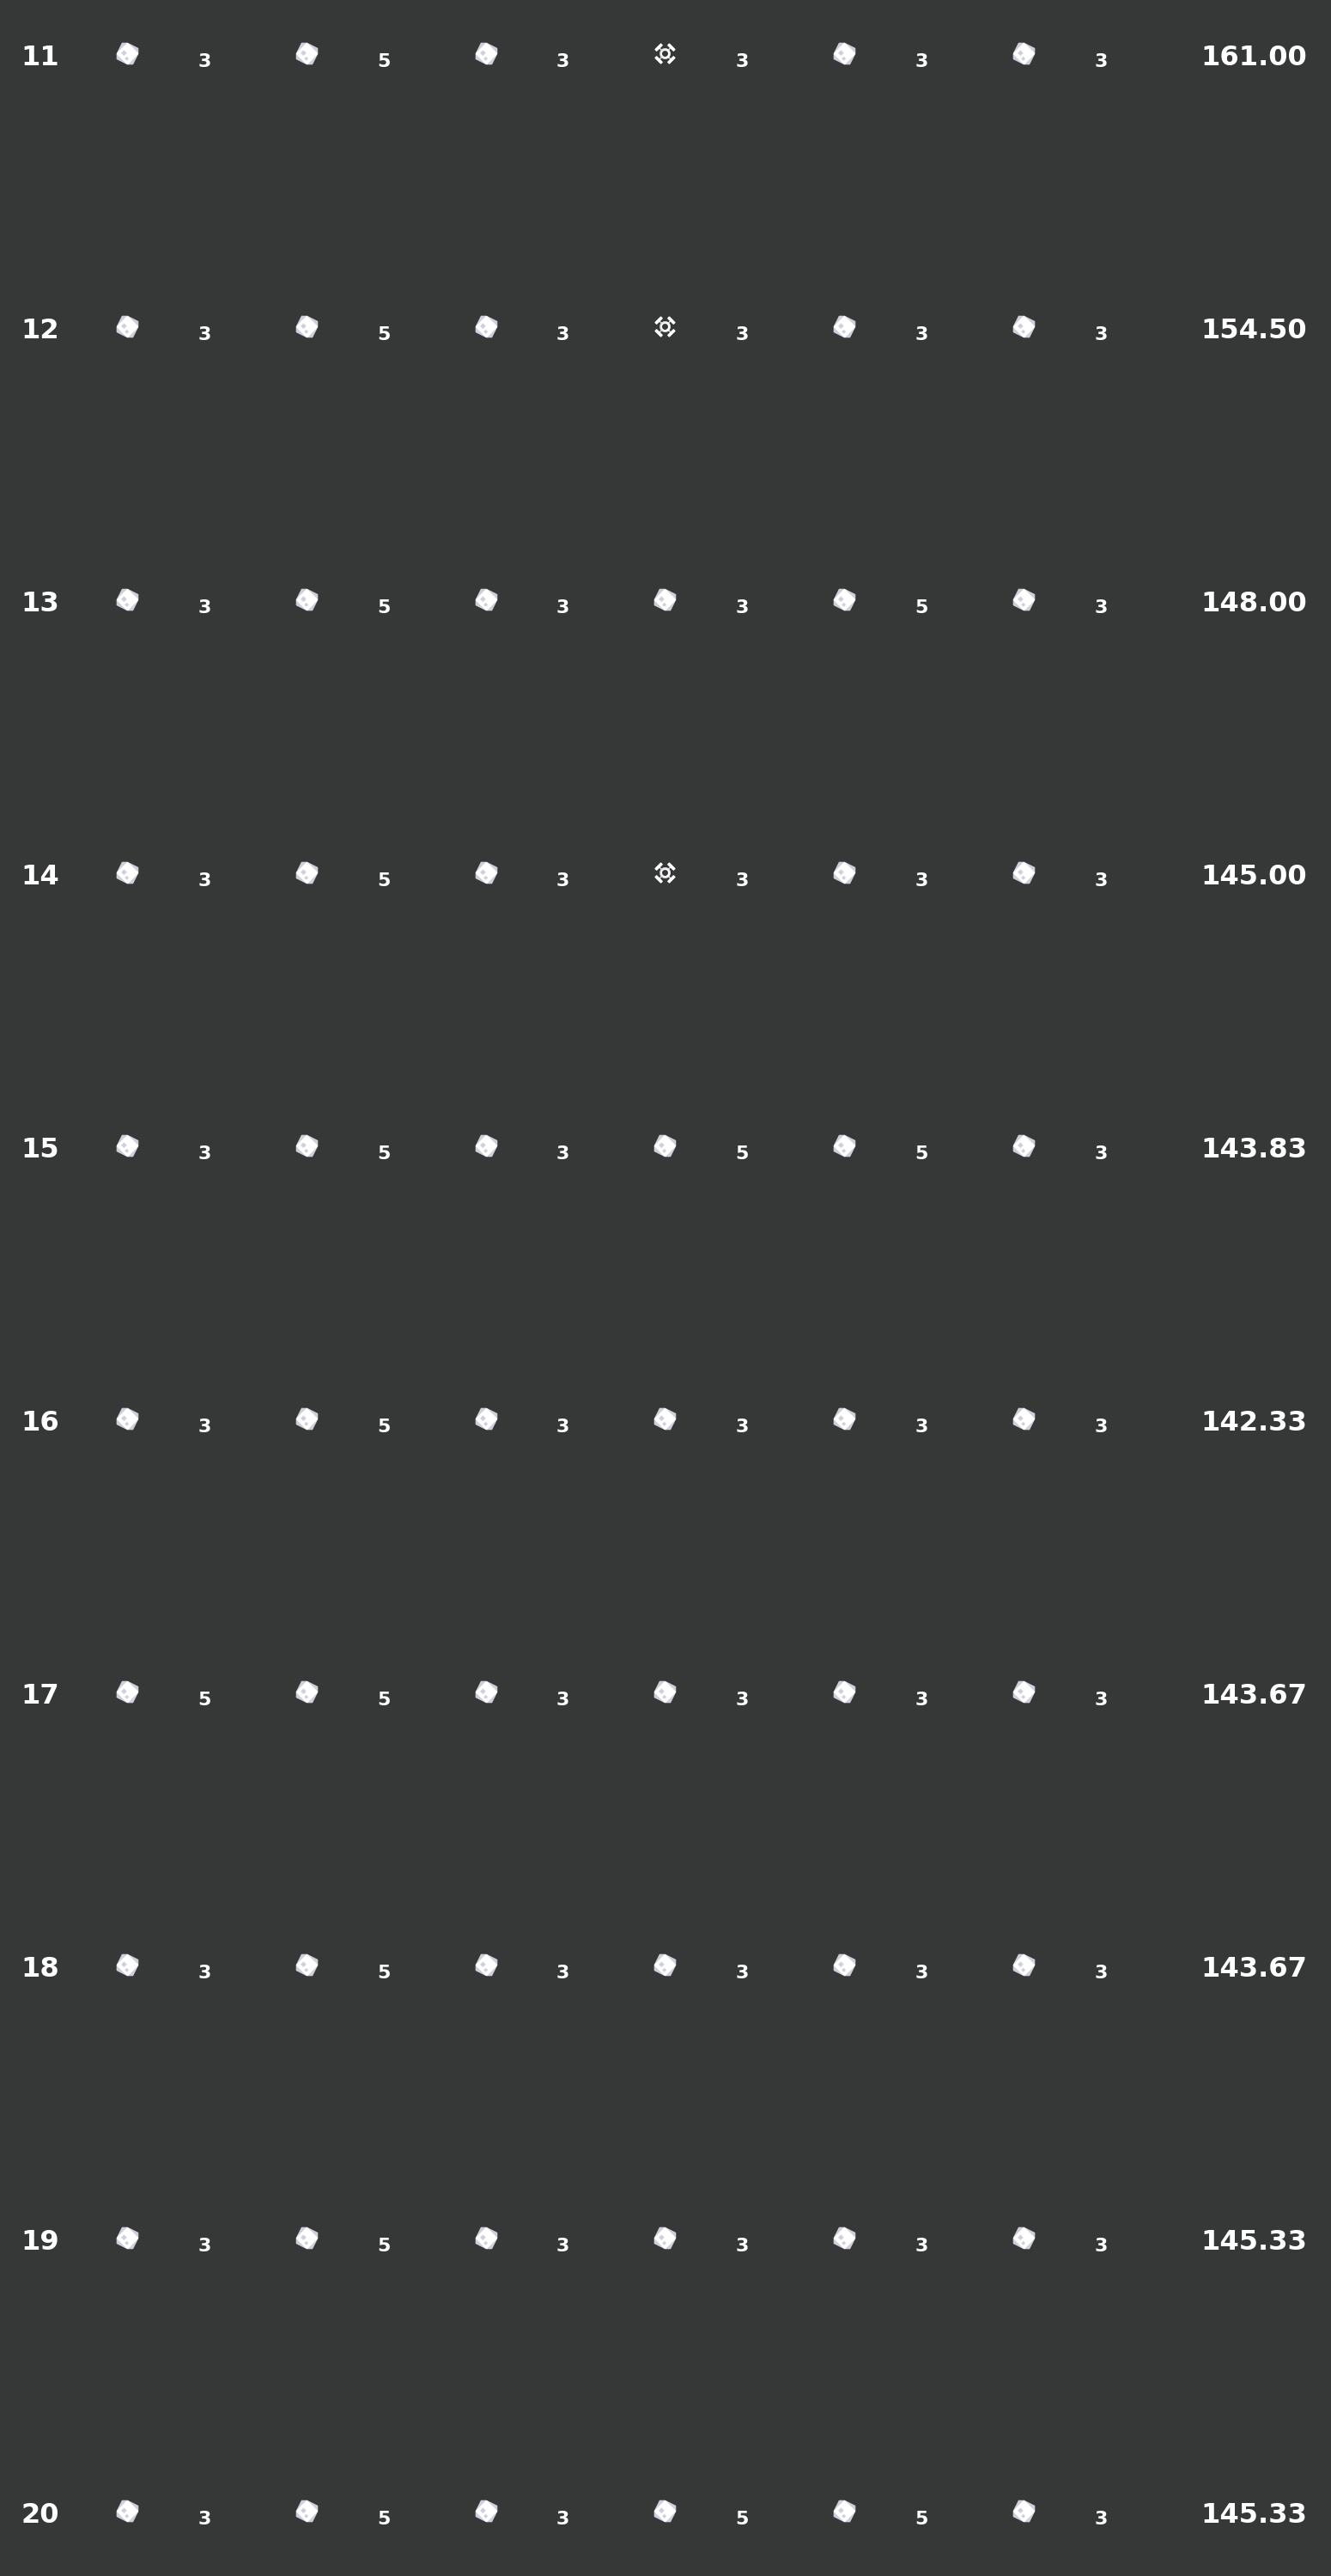
\includegraphics[width=0.7\textwidth]{figuras/ss/ss_yellowstill_ai_mode_2_2.png}
  \caption{Visualização da moda de cada onda com o fitness v3 contra Nave Parada, Disparo Amarelo.}
  \label{fig:ss-moda-ys-2-2}
\end{figure}

\begin{figure}[H]
  \centering
  \includegraphics[width=0.7\textwidth]{figuras/ss/ss_yellowstill_ai_mode_2_3.png}
  \caption{Visualização da moda de cada onda com o fitness v3 contra Nave Parada, Disparo Amarelo.}
  \label{fig:ss-moda-ys-2-3}
\end{figure}

%% ------------------------------------------------------------------------- %%
\section{Nave Movendo com Disparo Amarelo}
\label{sec:apend-moda-ss-ym-v3}

\begin{figure}[H]
  \centering
  \includegraphics[width=0.7\textwidth]{figuras/ss/ss_yellowmove_ai_mode_2_1.png}
  \caption{Visualização da moda de cada onda com o fitness v3 contra Nave Movendo, Disparo Amarelo.}
  \label{fig:ss-moda-ym-2-1}
\end{figure}

\begin{figure}[H]
  \centering
  \includegraphics[width=0.7\textwidth]{figuras/ss/ss_yellowstill_ai_mode_2_2.png}
  \caption{Visualização da moda de cada onda com o fitness v3 contra Nave Movendo, Disparo Amarelo.}
  \label{fig:ss-moda-ym-2-2}
\end{figure}

\begin{figure}[H]
  \centering
  \includegraphics[width=0.7\textwidth]{figuras/ss/ss_yellowstill_ai_mode_2_3.png}
  \caption{Visualização da moda de cada onda com o fitness v3 contra Nave Movendo, Disparo Amarelo.}
  \label{fig:ss-moda-ym-2-3}
\end{figure}

%% ------------------------------------------------------------------------- %%
\section{Nave Parada com Disparo Vermelho}
\label{sec:apend-moda-ss-rs-v3}

\begin{figure}[H]
  \centering
  \includegraphics[width=0.7\textwidth]{figuras/ss/ss_redstill_ai_mode_2_1.png}
  \caption{Visualização da moda de cada onda com o fitness v3 contra Nave Parada, Disparo Vermelho.}
  \label{fig:ss-moda-rs-2-1}
\end{figure}

\begin{figure}[H]
  \centering
  \includegraphics[width=0.7\textwidth]{figuras/ss/ss_redstill_ai_mode_2_2.png}
  \caption{Visualização da moda de cada onda com o fitness v3 contra Nave Parada, Disparo Vermelho.}
  \label{fig:ss-moda-rs-2-2}
\end{figure}

\begin{figure}[H]
  \centering
  \includegraphics[width=0.7\textwidth]{figuras/ss/ss_redstill_ai_mode_2_3.png}
  \caption{Visualização da moda de cada onda com o fitness v3 contra Nave Parada, Disparo Vermelho.}
  \label{fig:ss-moda-rs-2-3}
\end{figure}

%% ------------------------------------------------------------------------- %%
\section{Nave Movendo com Disparo Vermelho}
\label{sec:apend-moda-ss-rm-v3}

\begin{figure}[H]
  \centering
  \includegraphics[width=0.7\textwidth]{figuras/ss/ss_redmove_ai_mode_2_1.png}
  \caption{Visualização da moda de cada onda com o fitness v3 contra Nave Movendo, Disparo Vermelho.}
  \label{fig:ss-moda-rm-2-1}
\end{figure}

\begin{figure}[H]
  \centering
  \includegraphics[width=0.7\textwidth]{figuras/ss/ss_redmove_ai_mode_2_2.png}
  \caption{Visualização da moda de cada onda com o fitness v3 contra Nave Movendo, Disparo Vermelho.}
  \label{fig:ss-moda-rm-2-2}
\end{figure}

\begin{figure}[H]
  \centering
  \includegraphics[width=0.7\textwidth]{figuras/ss/ss_redmove_ai_mode_2_3.png}
  \caption{Visualização da moda de cada onda com o fitness v3 contra Nave Movendo, Disparo Vermelho.}
  \label{fig:ss-moda-rm-2-3}
\end{figure}
\par